\documentclass[hidelinks,a4paper,twoside,openright,12pt]{memoir}

%\includeonly{languages-without-case-competition}

%\setlrmarginsandblock{3.5cm}{3.5cm}{*}
%\setulmarginsandblock{3.5cm}{*}{1}
%\checkandfixthelayout

\usepackage{fenna-files/packages}
\addbibresource{fenna-files/references.bib}
\usepackage{fenna-files/abbreviations}

\makeatletter
\renewcommand{\@makeschapterhead}[1]{%
  {\noindent\raggedright\normalfont% Alignment and font reset
   \Huge\bfseries #1\par\nobreak}% Formatting
  \vspace{\baselineskip}% ...just a little space
}
\makeatother

\begin{document}

\bookmarksetup{startatroot}

\frontmatter

\begin{titlingpage}

\phantom{xx}

\newpage

\center
\large

\phantom{xx}

\vspace{3em}

{\LARGE
\tbf{Case competition in headless relatives}}\\

\vspace{5em}

Inauguraldissertation\\
zur Erlangung des Grades eines Doktors der Philosophie\\
im Fachbereich Neuere Philologien\\
der Johann Wolfgang Goethe-Universität\\
zu Frankfurt am Main\\

\vspace{5em}

vorgelegt von\\

\vspace{2em}

Fenna Bergsma\\
aus: Boarnsterhim, Niederlande\\

\vspace{3em}

2023\\

\vspace{1em}

1. Gutachterin: Prof. Dr. Katharina Hartmann\\
2. Gutachter: Dr. Pavel Caha\\

\vspace{1em}

Tag der mündlichen Prüfung: 17.12.2021


\end{titlingpage}

\chapter*[Acknowledgements]{Acknowledgements}

both supervisors: katharina (support, encouragment) and pavel (patience)

special thanks to pete (advice)

gk, pis and colleagues (zheng, heidi and derya)
stays abroad: penn and brno
conferences
people invited in frankfurt

\clearpage

\phantom{x}
\vspace{-7em}
\tableofcontents
\clearpage

\phantom{x}
\vspace{-7em}
\listoftables
\clearpage

\phantom{x}
\vspace{-7em}
\listoffigures
\clearpage

\chapter*[List of abbreviations]{List of abbreviations}
\begingroup
  \setlength{\LTleft}{-\tabcolsep}
\printacronyms[include=abbr, heading=none]
\endgroup
\addcontentsline{toc}{chapter}{List of abbreviations}
\clearpage

%%%%
\mainmatter
\setcounter{secnumdepth}{4}

% !TEX root = thesis.tex

\chapter{Introduction}

This dissertation is about case competition, a situation in which two cases are assigned but only one of them surfaces. One of the constructions in which case competition appears is relative clauses that lack a head, i.e. headless relatives.

% I show that one aspect about case competition in headless relatives holds for all languages (under discussion here at least). That is, there is a fixed order which decides which case wins the competition. I let this follow from what we observe in morphology. Another aspect of case competition in headless relatives differs per language. That is, whether the competition takes place to begin with. I connect this variable to the morphology of the language in question.
%
% Case competition in headless relatives has been described as some special property of a few special languages. Therefore, language-specific rules have been postulated to account for the data. My goal is to show that this phenomenon can be captured with `normal' syntactic processes, like ellipsis, c-command. The account makes predictions about how a language behaves based on the shape of its relative pronouns. And we see that case competition in headless relatives is actually more wide-spread than what has been assumed.
% %%this is too difficult

In this introduction I first introduce what I mean exactly with case competition in headless relatives. Then I introduce the topics I discuss in this dissertation.


\section{Introducing the title}

% First, case marks the grammatical role of the noun phrases. Case also appears on relative pronoun. Case on head can differ from case on relative pronoun. What happens if there is no noun? Two cases come together on the relative pronoun. What holds for all languages: there is a fixed order of who wins the competition. Specific from language to language: when does the competition take place?

Languages can use case to mark the grammatical role of a noun phrase in a clause \citep[cf.][]{moravcsik2009}. Consider the two Modern German sentences in \ref{ex:german-case}. What can descriptively be called the subject of the predicate \tit{mögen} `to like' is marked as nominative. What can be described as the object of \tit{mögen} `to like' is marked as accusative. The case marking of the noun phrases is reflected on the determiner in the noun phrase.
In \ref{ex:german-case-1}, \tit{der} in \tit{der Lehrer} `the teacher' appears in nominative case, because it is the descriptive subject in the clause. \tit{Den} in \tit{den Schüler} `the pupil' appears in accusative case, because it is a descriptive object of \tit{mögen} `to like'.
In \ref{ex:german-case-2}, the grammatical roles are reversed: \tit{der} in \tit{der Schüler} `the pupil' appears in nominative case, because it is the descriptive subject in the clause. \tit{Den} in \tit{den Lehrer} `the teacher' appears in accusative case, because it is the descriptive object of \tit{mögen} `to like'.

\ex.\label{ex:german-case}
\ag. Der Lehrer mag den Schüler.\\
 the.\ac{nom} teacher likes the.\ac{acc} student\\
 `The teacher likes the pupil.'\label{ex:german-case-1}
\bg. Der Schüler mag den Lehrer.\\
 the.\ac{nom} student likes the.\ac{acc} teacher\\
 `The pupil likes the teacher.'\label{ex:german-case-2}

Not only full noun phrases, but also other elements can be marked for case, such as relative pronouns. Modern German marks relative pronouns, just like full noun phrases, for the grammatical role they have in the clause. Consider the two sentences in \ref{ex:german-relatives}. These two sentences both contain a main clause that is modified by a relative clause.
In \ref{ex:german-relative-1}, the relative clause \tit{der nach draußen guckt} `that looks outside' modifies \tit{den Schüler} `the pupil'. \tit{Schüler} `pupil` is called the head (noun) or the antecedent of the relative clause. \tit{Den} in \tit{den Schüler} `the pupil` appears in accusative case, because it is the descriptive object of \tit{mögen} `to like' in the main clause. The relative pronoun \tit{der} `\ac{rel}.\ac{nom}.\ac{sg}.\ac{m}' appears in nominative case, because it is the descriptive subject of \tit{mögen} `to like' in the relative clause.

In \ref{ex:german-relative-2}, the relative clause \tit{den er beim Verstecktspiel sucht} `that he is searching for playing hide-and-seek' modifies \tit{den Schüler} `the pupil'. \tit{Den} in \tit{den Schüler} `the pupil` appears again in accusative, because it is the descriptive object of \tit{mögen} `to like' in the main clause. The relative pronoun \tit{den} `\ac{rel}.\ac{acc}.\ac{sg}.\ac{m}' appears in accusative case, because it is the descriptive object of \tit{suchen} `to search' in the relative clause.

\ex.\label{ex:german-relatives}
\ag. Der Lehrer mag den Schüler, der nach draußen guckt.\\
 the.\ac{nom} teacher likes the.\ac{acc} student \ac{rel}.\ac{nom}.\ac{sg}.\ac{m} to outside looks\\
 `The teacher likes the pupil that is looking outside.'\label{ex:german-relative-1}
 \bg. Der Lehrer mag den Schüler, den er beim Versteckspiel sucht.\\
 the.\ac{nom} teacher likes the.\ac{acc} student \ac{rel}.\ac{acc}.\ac{sg}.\ac{m} he {at the} {hide-and-seek game} searches\\
 `The teacher likes the pupil that he is searching for playing hide-and-seek.'\label{ex:german-relative-2}

Compare the two sentences in \ref{ex:german-relatives}. In both sentences the head is marked as accusative because it is the descriptive object in the main clause. The case of the relative pronoun in \ref{ex:german-relative-2} is also accusative, because it is the descriptive object in the relative clause. The case of the relative pronoun in \ref{ex:german-relative-1} is nominative, because it is the descriptive subject in the relative clause. So, the case of the relative pronoun in \ref{ex:german-relative-1} differs from the case of the head.

The focus of this dissertation lies on headless relatives. As the name suggests, this type of relative clause lacks a head.\footnote{
This `missing noun' has been interpreted in two different ways. Some researchers argue that the noun is truly missing, it is absent, cf. \citealt{citko2005,vanriemsdijk2006}. Others claim that there is actually a head, but it is phonologically zero, \citealt{bresnan1978,groos1981,grosu2003}. At this point in the discussion this distinction is not relevant. I return to the issue in Chapter \ref{ch:connecting}.
}
Even though Modern German also has case competition in headless relatives, I turn to Gothic now. The patterns among the two languages differ slightly, and the first part of the dissertation can be illustrated best with Gothic.

I give an example of a headless relative in Gothic in \ref{ex:gothic-acc-acc}.
There is no head that this relative clause modifies, because it is a headless relative. This is different from the examples from German I gave above, which each had a head.
The predicate \tit{arman} `to pity' takes accusative objects, as indicated by the subscript on the gloss of the verb. The predicate \tit{gaarman} `to pity' also takes accusative objects, indicated again by the subscript.
The relative pronoun \tit{þan(a)} `\ac{rel}.\ac{acc}.\ac{sg}.\ac{m}' appears in accusative case.\footnote{
The relative pronoun without the complementizer \tit{-ei} is \tit{þana}. Therefore, I refer to the relative pronoun as \tit{þan(a)}.
}

\exg. gaarma þan -ei arma\\
 pity.\ac{pres}.1\ac{sg}\scsub{[acc]} \ac{rel}.\ac{acc}.\ac{sg}.\ac{m} -\ac{comp} pity.\ac{pres}.1\ac{sg}\scsub{[acc]}\\
 `I pity him whom I pity' \flushfill{Gothic, \ac{rom} 9:15, adapted from \pgcitealt{harbert1978}{339}}\label{ex:gothic-acc-acc}

Where does this accusative case come from? Logically speaking, there are two possible sources: the predicate in the main clause \tit{gaarman} `to pity', the predicate in the relative clause \tit{arman} `to pity'. From now on, I use the terms internal and external case to refer to these two possible case sources. Now there are three logical possibilities for the source of the accusative case on \tit{þan(a)} `\ac{rel}.\ac{acc}.\ac{sg}.\ac{m}' in \ref{ex:gothic-acc-acc}: the internal case, the external case, or both.

Internal case refers to the case associated with the relative pronoun internal to the relative clause. More precisely, it is the case, which is associated with the grammatical role that the relative pronoun has internal to the relative clause. In \ref{ex:gothic-acc-acc}, the relative pronoun is the descriptive object of \tit{arman} `to pity'. The predicate \tit{arman} `to pity' takes accusative objects. So, the internal case is accusative.

External case refers to the case associated with the missing head in the main clause, which is external to the relative clause. Concretely, it is the case which is associated with the grammatical role that the missing head has external to the relative clause. In \ref{ex:gothic-acc-acc}, the missing head is the descriptive object of \tit{gaarman} `to pity'. The predicate \tit{gaarman} `to pity' takes accusative objects. In \ref{ex:gothic-acc-acc}, the external case is accusative.

Now I return to the question where \tit{þan(a)} `\ac{rel}.\ac{acc}.\ac{sg}.\ac{m}' in \ref{ex:gothic-acc-acc} got its case from. In the remainder of this section I show evidence for the claim that the relative pronoun is sensitive to both the internal and the external case.
This is easy to imagine for the internal case: the internal case reflects the grammatical role of the relative clause. It is a bit more complicated for the external case. The external case is associated with the grammatical role of the missing head in the main clause. The idea is going to be that the external case cannot be reflected on a non-existing head. Indirectly, it appears on the relative pronoun.\footnote{
Later on I will argue that this indirect process is actually a deletion operation.
}
This means that the internal and external case come together on the relative pronoun. In other words, there is case competition going on in headless relatives. \ref{ex:gothic-acc-acc} is indeed the first example I gave of case competition in a headless relative. It is an uninteresting one, because the two competing cases are identical.

Consider the example in \ref{ex:gothic-acc-nom}, in which the internal case is accusative and the external case is nominative.
The internal case is accusative. The predicate \tit{frijon} `to love' takes accusative objects, as indicated by the subscript on the predicate.
The external case is accusative. The predicate \tit{wisan} `to be' takes nominative subjects, indicated by the subscript on the predicate.
The relative pronoun \tit{þan(a)} `\ac{rel}.\ac{acc}.\ac{sg}.\ac{m}' appears in accusative. This accusative can only come from the predicate \tit{frijon} `to love', which is the internal case here. The relative pronoun is marked in bold, just as the relative clause, showing that the relative pronoun patterns with the relative clause.

\exg. \tbf{þan} \tbf{-ei} \tbf{frijos} siuks ist\\
 \ac{rel}.\ac{acc}.\ac{sg}.\ac{m} -\ac{comp} love.\ac{pres}.2\ac{sg}.\scsub{[acc]} sick be.\ac{pres}.3\ac{sg}\scsub{[nom]}\\
 `the one whom you love is sick' \flushfill{Gothic, \ac{john} 11:3, adapted from \pgcitealt{harbert1978}{342}}\label{ex:gothic-acc-nom}

The conclusion that follows is that the relative pronoun can take the internal case. At this point it remains unclear what happened to the external nominative case.

Now consider the example in \ref{ex:gothic-nom-acc}, in which the internal case is nominative and the external case is accusative.
The internal case is nominative. The predicate \tit{wisan} `to be' takes nominative subjects, as indicated by the subscript on the predicate.
The external case is accusative. The predicate \tit{ussiggwan} `to read' takes accusative objects, as indicated by the subscript on the predicate.
The relative pronoun \tit{þo} `\ac{rel}.\ac{acc}.\ac{sg}.\ac{n}' appears in the accusative case. This accusative can only come from the predicate \tit{ussiggwan} `to read', which is the external case here. The relative pronoun is not marked in bold, just like as the main clause, showing that the relative pronoun patterns with the main clause.

\exg. jah þo \tbf{-ei} \tbf{ist} \tbf{us} \tbf{Laudeikaion} jus ussiggwaid\\
 and \ac{rel}.\ac{acc}.\ac{sg}.\ac{n} -\ac{comp} be.\ac{pres}.3\ac{sg}\scsub{[nom]} from Laodicea you.\ac{pl} read.?.\scsub{[acc]}\\
 `and you read the one which is from Laodicea' \flushfill{Gothic, \ac{col} 4:16, adapted from \pgcitealt{harbert1978}{357}}\label{ex:gothic-nom-acc}

The conclusion that follows is that the relative pronoun can take the external case. At this point it remains unclear what happened to the internal nominative case.

The examples in \ref{ex:gothic-acc-nom} and \ref{ex:gothic-nom-acc} have shown that the relative pronoun in headless relatives can take either the internal or the external case. In the examples, the predicates take nominative and accusative, and in both cases, the relative pronoun appeared in accusative case. In other words, there was a competition between nominative and accusative, and accusative won.

In the next section, I discuss the content of this dissertation. Before that, I comment on two notational conventions I use throughout this dissertation. First, I place subscripts on the glosses of the predicates. They indicate what the internal or external case is. The subscript on the predicate in the relative clause indicates the internal case. The subscript on the predicate in the main clause indicates the external case. This subscript can mean different things.
For \tit{frijon} `to love' in \ref{ex:gothic-acc-nom} the subscript indicates which case the complement of the verb appears in. The subscript on \tit{wisan} `to be' in \ref{ex:gothic-acc-nom} refers to the case the descriptive subject appears in. A subscript can also refer to the case of the indirect object of a predicate, a possibility that arises in the next chapter.
In other words, the subscript can refer several elements: a subject, direct object or indirect object of a predicate. There is no overarching theoretical notion that the subscript makes reference to. The subscript simply indicates which case is required within the (main or relative) clause.

Second, I write the relative clause in bold. When the relative pronoun takes the internal case, I mark it in bold as well, as shown in \ref{ex:gothic-acc-nom}. When the relative pronoun takes the external case, I leave it black, indicating it patterns with the main clause. An example of that is \ref{ex:gothic-nom-acc}.


\section{The content of this dissertation}

In the previous section I introduced the notion of case competition, and I illustrated how it appears in headless relatives. This dissertation discusses two question regarding this phenomenon.
The first one is which case is going to win the case competition, i.e. which case surfaces. I discuss this in Part \ref{part:complexity}.
The second question is whether both competitors are able to compete in the competition, i.e. whether one of the cases is surfacing or both are ungrammatical. I discuss this in Part \ref{part:direction}.
For both I will show that morphology is leading. What we observe in syntax is a reflex of the morphology.

% In Part \ref{part:complexity} I discuss the pattern observed in headless relatives in Gothic. This pattern has also been described for German, Greek, etc. etc. references references.
% The pattern that arises in headless relatives is not restricted to headless relatives. It can also be observed in another syntactic phenomenon: the accessiblity hierarchy. This is..
% Lastly: the pattern we observe in these two syntactic phenomena is what we know from morphology. I discuss patterns in morphology: formal containment, syncretism patterns, suppletion patterns.
%
% In Part \ref{part:complexity} I discuss an aspect of headless relatives that differs per language. That is, not all languages act like Gothic.
%
% \ex. Modern German
% \ag. accusative dative\\
%  \\
%  `'
% \bg. dative accusative\\
%  \\
%  `'
%
%  \ex. Old High German
%  \ag. accusative dative\\
%   \\
%   `'
%  \bg. dative accusative\\
%   \\
%   `'
%
%   \ex. Italian
%   \ag. accusative dative\\
%    \\
%    `'
%   \bg. dative accusative\\
%    \\
%    `'
%
% So far people said..
% I connect this crosslinguistic variation to morphology.. so i reduce it to differences in the lexicon
%
% In Part \ref{part:details} I show how all of this can be derived in derivations.


\part{Case competition}\label{part:case-facts}
% !TEX root = thesis.tex

\chapter{A recurring pattern}\label{ch:recurring}

This chapter introduces the pattern that forms the focus of the first part of the dissertation. In Section \ref{sec:pattern-rels} I show that case competition in headless relatives adheres to the case scale in \ref{ex:case-scale-intro}.

\ex. \ac{nom} < \ac{acc} < \ac{dat}\label{ex:case-scale-intro}

Then I show that this pattern is not unique to headless relatives. It appears in more syntactic and morphological phenomena. Section \ref{sec:impl-hier} discusses two implicational hierarchies that show the same case ordering. The hierarchies concern agreement and relativization across languages. Section \ref{sec:case-morphology} shows that the case scale also shows up in morphological patterns. It can be observed in patterns of syncretism and in morphological containment.


\section{In headless relatives}\label{sec:pattern-rels}

As the name suggests, headless relatives are relative clauses that lack an (overt) head. The internal case, the case from the relative clause, and the external case, the case from the main clause, compete to surface on the relative pronoun. It has been argued in the literature that the two competing cases always adhere a to particular case scale \citep[cf.][]{harbert1978,pittner1995,vogel2001,grosu2003,caha2019,bergsma2019}. This is the scale I gave in the introduction, repeated here in \ref{ex:case-scale}. Elements more to the right on this scale win over elements more to the left on this scale.\footnote{
In the literature about headless relatives, the genitive is often discussed together with the nominative, accusative and dative \citep[cf.][]{harbert1978,pittner1995}. In this dissertation I do not discuss the genitive. The reason is that I restrict myself to cases that appear in all possible case competition combinations. As the genitive does not fulfill that requirement, it is therefore excluded. In Chapter \ref{ch:conclusion} I briefly return to the issue.
}

\ex. \ac{nom} < \ac{acc} < \ac{dat}\label{ex:case-scale}

This can be reformulated as follows. In a competition, dative wins over accusative, and dative wins over nominative. Additionally, accusative wins over nominative. In this section I illustrate this scale with examples. When two cases compete, the relative pronoun always appears in the case more to the right on the case scale. It does not matter whether it is the internal or the external case. I illustrate this with examples from headless relatives in Gothic \citep{harbert1978}.

I start with the competition between dative and accusative. Following the case scale in \ref{ex:case-scale}, the relative pronoun appears in dative case and never in accusative.

Consider the example in \ref{ex:gothic-acc-dat-rep}, repeated from the introduction. In this example, the internal case is dative and the external case is accusative.
The internal case is dative. The preposition \tit{ana} `on' takes dative complements.
The external case is accusative. The predicate \tit{ushafjands} `picking up' takes accusative objects.
The relative pronoun \tit{þamm(a)} `\ac{rel}.\ac{dat}.\ac{n}.\ac{sg}' appears in the internal case: the dative. The relative pronoun is marked in bold, just like as the relative clause, showing that the relative pronoun patterns with the relative clause.
Examples in which the internal case is dative, the external case is accusative and the relative pronoun appears in accusative case are unattested.

\exg. ushafjands \tbf{ana} \tbf{þamm} \tbf{-ei} \tbf{lag}\\
 {picking up}\scsub{[acc]} on\scsub{[dat]} \ac{rel}.\ac{dat}.\ac{n}.\ac{sg} -\ac{comp} lay\\
 `picking up (that) on what he lay' \flushfill{Gothic, \ac{luke} 5:25, adapted from \pgcitealt{harbert1978}{343}}\label{ex:gothic-acc-dat-rep}

%aiþþau ƕaiwa galaubjand þammei ni hausidedun
% ei galeikai þammei drauhtinoþ


% ushafjands
% Present participle: Strong Masculine Nominative Singular
% Lemma us-hafjan
% `erheben'
%
% lag
% Active Indicative Preterite 3rd Person Singular
% Lemma ligan
% `liegen'

Consider the example in \ref{ex:gothic-dat-acc-rep}, repeated from the introduction. In this example, the internal case is accusative and the external case is dative.
The internal case is accusative. The predicate \tit{jains} `sent' takes accusative objects.
The external case is dative. The predicate \tit{galaubjaiþ} `believe' takes dative objects.
The relative pronoun \tit{þamm(a)} `\ac{rel}.\ac{dat}.\ac{m}.\ac{sg}' appears in the external case: the dative. The relative pronoun is not marked in bold, just like as the main clause, showing that the relative pronoun patterns with the main clause.
Examples in which the internal case is accusative, the external case is dative and the relative pronoun appears in accusative case are unattested.

\exg. ei galaubjaiþ þamm \tbf{-ei} \tbf{insandida} \tbf{jains}\\
that believe\scsub{[dat]} \ac{rel}.\ac{dat}.\ac{m}.\ac{sg} -\tsc{comp} {sent}\scsub{[acc]} he\\
`that you believe on (him) whom he has sent' \flushfill{Gothic, \ac{john} 6:29, my translation}\label{ex:gothic-dat-acc-rep}

% Lemma ga-laubjan
% 1. glauben 2. anvertrauen
% Active Optative Present 2nd Person Plural
%
% Lemma in-sandjan
% entsenden
% Active Indicative Preterite 3rd Person Singular
%
% Lemma jains
% Pronoun, demonstrative  jener
% Strong Masculine Nominative Singular

I continue with the competition between dative and nominative. Following the case scale in \ref{ex:case-scale}, the relative pronoun appears in dative case and never in nominative.

Consider the example in \ref{ex:gothic-dat-nom}, in which the internal case is dative and the external case is nominative.
The internal case is dative. The predicate \tit{fraletada} `is forgiven' takes dative objects.
The external case is nominative. The predicate \tit{frijod} `loves' takes nominative subjects.
The relative pronoun \tit{þamm(a)} `\ac{rel}.\ac{dat}.\ac{m}.\ac{sg}' appears in the internal case: the dative. The relative pronoun is marked in bold, just as the relative clause, showing that the relative pronoun patterns with the relative clause.
Examples in which the internal case is dative, the external case is nominative and the relative pronoun appears in nominative case are unattested.

\exg. iþ \tbf{þamm} \tbf{-ei} \tbf{leitil} \tbf{fraletada} leitil frijod\\
 but \ac{rel}.\ac{dat}.\ac{m}.\ac{sg} -\ac{comp} little {is forgiven}\scsub{[dat]} little loves\scsub{[nom]}\\
 `but the one whom little is forgiven loves little' \flushfill{Gothic, \ac{luke} 7:47, adapted from \pgcitealt{harbert1978}{342}}\label{ex:gothic-dat-nom}

% Lemma leitils
% klein, wenig
% Strong Neuter Nominative Singular
% Strong Neuter Accusative Singular
%
% Lemma fra-letan
% lassen; frei lassen, entlassen; unterlassen; zulassen, erlauben; erlassen, vergeben; herablassen
% Passive Indicative Present 1st Person Singular
% Passive Indicative Present 3rd Person Singular
%
% frijod: ??

Consider the example in \ref{ex:gothic-nom-dat}, in which the internal case is nominative and the external case is dative.
The internal case is nominative. The predicate \tit{sind fraþjaiþ} `are above' takes a nominative subject.
The external case is dative. The predicate \tit{fraþjaiþ} `think on' takes dative indirect objects.
The relative pronoun \tit{þaim} `\ac{rel}.\ac{dat}.\ac{pl}.\ac{n}' appears in the external case: the dative. The relative pronoun is not marked in bold, just like as the main clause, showing that the relative pronoun patterns with the main clause.
Examples in which the internal case is nominative, the external case is dative and the relative pronoun appears in nominative case are unattested.

\exg. þaim \tbf{-ei} \tbf{iupa} \tbf{sind} fraþjaiþ \\
 \ac{rel}.\ac{dat}.\ac{pl}.\ac{n} -\ac{comp} above are\scsub{[nom]} {think on}\scsub{[dat]}\\
 `set your mind on those which are above' \flushfill{Gothic, \ac{col} 3:2, adapted from \pgcitealt{harbert1978}{339}}\label{ex:gothic-nom-dat}

% Lemma iupa
% oben
%
% Lemma wisan
% sein
% Active Indicative Present 3rd Person Plural
%
% Lemma fraþjan
% 1. denken 2. erkennen, verstehn 3. verständig sein
% Active Optative Present 2nd Person Plural

I end with the competition between accusative and nominative. Following the case scale in \ref{ex:case-scale}, the relative pronoun appears in accusative case and never in nominative.

Consider the example in \ref{ex:gothic-acc-nom}, in which the internal case is accusative and the external case is nominative.
The internal case is accusative. The predicate \tit{frijos} `love' takes accusative objects.
The external case is nominative. The predicate \tit{siuks ist} `is sick' takes nominative subjects.
The relative pronoun \tit{þan(a)} `\ac{rel}.\ac{acc}.\ac{m}.\ac{sg}' appears in the internal case: the accusative. The relative pronoun is marked in bold, just like as the relative clause, showing that the relative pronoun patterns with the relative clause.
Examples in which the internal case is accusative, the external case is nominative and the relative pronoun appears in nominative case are unattested.

\exg. \tbf{þan} \tbf{-ei} \tbf{frijos} siuks ist\\
 \ac{rel}.\ac{acc}.\ac{m}.\ac{sg} -\ac{comp} love\scsub{[acc]} sick is\scsub{[nom]}\\
 `the one whom you love is sick' \flushfill{Gothic, \ac{john} 11:3, adapted from \pgcitealt{harbert1978}{342}}\label{ex:gothic-acc-nom}

% Lemma frijon
% lieben
% Active Indicative Present 2nd Person Singular
%
% Lemma siuks
% krank, schwach
% Strong Masculine Nominative Singular
%
% Lemma wisan
% sein, dasein, existieren
% Active Indicative Present 3rd Person Singular

Consider the example in \ref{ex:gothic-nom-acc}, in which the internal case is nominative and the external case is accusative.
The internal case is nominative. The predicate \tit{ist us Laudeikaion} `is from Laodicea' takes nominative subjects.
The external case is accusative. The predicate \tit{ussiggwaid} `read' takes accusative objects.
The relative pronoun \tit{þo} `\ac{rel}.\ac{acc}.\ac{n}.\ac{sg}' appears in the external case: the accusative. The relative pronoun is not marked in bold, just like as the main clause, showing that the relative pronoun patterns with the main clause.
Examples in which the internal case is nominative, the external case is accusative and the relative pronoun appears in nominative case are unattested.

\exg. jah þo \tbf{-ei} \tbf{ist} \tbf{us} \tbf{Laudeikaion} jus ussiggwaid\\
 and \ac{rel}.\ac{acc}.\ac{n}.\ac{sg} -\ac{comp} is\scsub{[nom]} from Laodicea you read\scsub{[acc]}\\
 `and read that which is from Laodicea' \flushfill{Gothic, \ac{col} 4:16, adapted from \pgcitealt{harbert1978}{357}}\label{ex:gothic-nom-acc}

% Lemma wisan
% sein, dasein, existieren
% Active Indicative Present 3rd Person Singular
%
% Lemma us +dat?
% [m. Dat.] aus, von
%
% Lemma þu
% du
% Nominative Plural
%
% ussiggwaid
% read? stem is ussiggw?

A summary of the Gothic data as a whole is given in Table \ref{tbl:summary-gothic}. The left column shows the internal case between square brackets. The upper row shows the external case between square brackets. The other cells indicate the case of the relative pronoun. The diagonal is left blank, because these are instances in which the internal and external case match.
The remaining six cells show instances where the internal and external case differ. Within the cells, two cases are given. The case in the lower left corner stands for the relative pronoun in the internal case. The case in the upper right corner stands for the relative pronoun in the external case. The grammatical examples are marked in gray. The unattested examples are marked with an asterix and are unmarked.\footnote{
Throughout this dissertation * stands for 'not found in natural language'. For extinct languages this means that there are no attested examples. For modern languages it means that the examples are ungrammatical.
}

\begin{table}[ht]
  \center
  \caption {Case competition in Gothic headless relatives}
    % !TEX root = thesis.tex

\begin{table}[H]
  \center
  \caption {Case attraction in headless relatives in Gothic}
    \begin{tabular}{c|c|c|c}
      \toprule
        \diagbox[linecolor=white]{\ac{int}}{\ac{ext}}
            & [\ac{nom}]
            & [\ac{acc}]
            & [\ac{dat}]
            \\ \cmidrule{1-4}
        [\ac{nom}]
            & \colorbox{LG}{\ac{nom}}
            & \diagbox[linecolor=white]{*\ac{nom}}{\colorbox{DG}{\ac{acc}}}
            & \diagbox[linecolor=white]{*\ac{nom}}{\colorbox{DG}{\ac{dat}}}
            \\ \cmidrule{1-4}
        [\ac{acc}]
            & \diagbox[linecolor=white]{\colorbox{DG}{\ac{acc}}}{*\ac{nom}}
            & \colorbox{LG}{\ac{acc}}
            & \diagbox[linecolor=white]{*\ac{acc}}{\colorbox{DG}{\ac{dat}}}
            \\ \cmidrule{1-4}
        [\ac{dat}]
            & \diagbox[linecolor=white]{\colorbox{DG}{\ac{dat}}}{*\ac{nom}}
            & \diagbox[linecolor=white]{\colorbox{DG}{\ac{dat}}}{*\ac{acc}}
            & \colorbox{LG}{\ac{dat}}
            \\
      \bottomrule
    \end{tabular}
\end{table}

    \label{tbl:summary-gothic}
\end{table}

The three instances in the lower left corner correspond to the examples \ref{ex:gothic-acc-nom}, \ref{ex:gothic-dat-nom} and \ref{ex:gothic-dat-acc-rep}. In the attested examples, the relative pronoun appears in the internal case.
The three instances in the upper right corner correspond to the examples in \ref{ex:gothic-nom-acc}, \ref{ex:gothic-nom-dat} and \ref{ex:gothic-acc-dat-rep}. In the attested examples, the relative pronoun appears in the external case.

\begin{table}[ht]
  \center
  \caption {Summary of Gothic matching headless relative data}
    % !TEX root = ../thesis.tex

\begin{tabular}{c|c|c|c}
  \toprule
      \textsubscript{\ac{int}} \textsuperscript{\ac{ext}}
        & [\ac{nom}]
        & [\ac{acc}]
        & [\ac{dat}]
        \\ \cmidrule{1-4}
    [\ac{nom}]
        &
        & \ac{acc}
        & \ac{dat}
        \\ \cmidrule{1-4}
    [\ac{acc}]
        & \ac{acc}
        &
        & \ac{dat}
        \\ \cmidrule{1-4}
    [\ac{dat}]
        & \ac{dat}
        & (\ac{dat})
        &
        \\
  \bottomrule
\end{tabular}

    \label{tbl:summary-gothic-1}
\end{table}

To sum up, case competition in headless relative is subject to the case scale, repeated in \ref{ex:case-scale-rep}.

\ex. \ac{nom} < \ac{acc} < \ac{dat}\label{ex:case-scale-rep}

If two cases compete, dative wins over accusative and nominative, and accusative wins over nominative. In this section I gave examples from Gothic that illustrate this. As I mentioned in the introduction of this section, this case scale is not specific for Gothic, but it holds across languages (cf. see \citealt{pittner1995} for Modern, Middle High and Old High German, \citealt{grosu2003} for Ancient Greek and \citealt{daskalaki2011} for Modern Greek).\footnote{
These languages differ from Gothic in that they are subject to an additional constraint. That is, they only allow either the internal or the external case to win case competitions. If the other case is more to the right on the case scale \ref{ex:case-scale-rep}, the result is ungrammatical.
Old High German is an example of a language that only allows the external case to win the case competition. If the internal case is more to the right on the case scale, the headless relative is ungrammatical. Modern German is an example of a language that only allows the internal case to win the case competition. If the external case is more to the right on the case scale, the headless relative is ungrammatical.
This topic is the main focus of Part \ref{part:complexity} of this dissertation.}

In the remainder of this chapter I show that headless relatives are not the only place where the case scale shows up. Instead, it appears with more syntactic phenomena. Moreover, exactly this scale is also reflected in morphology.

% The nativeness of the headless relative constructions under
% consideration, and in particular those represented by group (I), can be
% established for the moment by citing instances in which they occur independently
% of the Greek, e.g., in which the Gothic modified relative clause
% reflects a Greek participial construction or a noun, or instances in which
% 18
% they occur in opposition to the Greek. Evidence of the first type is
% found in Mk 10:32, Luk 3:13, Rom 14:19, II Cor 8:11, Col 3:2, and elsewhere.



\section{In syntax}\label{sec:impl-hier}

In this section I discuss two additional syntactic phenomena that reflect the \ac{nom} < \ac{acc} < \ac{dat} scale. The first one is an implicational hierarchy that concerns agreement. The second one is an implicational hierarchy about relativization.


\subsection{Agreement}

Agreement can be seen as ``a systematic covariance between a semantic or formal property of one element and a formal property of another'' \citep{steel1978}. Put differently, the shape of one element changes according to some properties of an element it relates to. In this section I discuss the agreement between a predicate and its arguments.

It differs per language with how many of its arguments a predicate agrees. However, it is not random with which agreement takes place. Instead, there is an implicational hierarchy that is identical to the one observed for headless relatives: \ac{nom} < \ac{acc} < \ac{dat}.

\citet{moravcsik1978} formulated the implicational hierarchy in terms of grammatical functions subject, direct object and indirect object.\footnote{
\citet{moravcsik1978} also included adverbs on the lowest end of the hierarchy. I leave them out here, because they are not relevant for the discussion.
}
The hierarchy is schematically represented in Figure \ref{fig:agr-sub-do-io}. It should be read as follows: if a language allows the predicate to agree with the argument in a particular circle, it also allows the predicate to agree with the argument in the circle around it.

\begin{figure}[ht]
  \centering
  \begin{tikzpicture}
    \draw (0,1) circle (2.25);
    \draw [fill opacity=0.4, fill=LG] (0,0.5) circle (1.75);
    \draw [fill opacity=0.4, fill=DG] (0,0) circle (1.25);

    \node[] at (0,2.75) {subject};
    \node[] at (0,1.5) {direct object};
    \node[align=center] at (0,0) {indirect\\ object};
  \end{tikzpicture}
  \caption{\posscitealt{moravcsik1978} schema}
  \label{fig:agr-sub-do-io}
\end{figure}

Then, there are four types of languages possible: first, a language that does not show any agreement; second, a language that shows agreement only with the subject and not with the direct and indirect object; third, a language that shows agreement with the subject and direct object but not with the indirect object; and fourth, a language that shows agreement with the subject, the direct object and the indirect object.

The implicational hierarchy holds for languages, not for sentences. That is, it is not the case that in a language of a particular type all instances of the grammatical function show agreement. To be more precise, in a language of the second type, that only shows agreement with the subject, not all subjects have to show agreement. Particular types of subject, such as experiencer subjects often do not show any agreement.

Japanese is an example of a language that does not show any agreement on the predicate. An example is given in \ref{ex:japanese-agr}. The predicate \tit{okutta} `sent' does not agree with the subject \tit{Tarooga} `Taro', with the direct object \tit{nimotuo} `package' or with the indirect object \tit{Hanakoni} `Hanako'.

\exg. Taroo-ga Hanako-ni nimotu-o okutta.\\
 Taro-\ac{nom} Hanako-\ac{dat} package-\ac{acc} sent\\
 `Taro sent Hanako a package.' \flushfill{Japanese, \pgcitealt{miyagawa2004}{5}}\label{ex:japanese-agr}

German is an example of a language that shows agreement with the subject of the clause. An example is given in \ref{ex:german-agr}. The predicate \tit{gibst} `give' contains the morpheme \tit{-st}, marked in bold. This morpheme is the agreement morpheme for second person singular subjects (in the present tense). The predicate \tit{gibst} `give' agrees in person and number with the subject \tit{du} `you'. There is no agreement with the direct object \tit{das Buch} `the book' or the indirect object \tit{mir} `me'.

\exg. Du gib \tbf{-st} mir das Buch.\\
 you give -2\ac{sg}.\ac{pres} me the book\\
 `You give me the book.' \flushfill{German}\label{ex:german-agr}

Hungarian is an example of a language that shows agreement with the subject and the direct object of a clause. An example is given in \ref{ex:hungarian-agr}. The predicate \tit{adom} `give' contains the morpheme \tit{-om}, marked in bold. This is a portmonteau morpheme for a first person singular subject and a third person object agreement. The predicate \tit{adom} `give' agrees with the subject \tit{én} `I' and the direct object \tit{a könyvet} `the book'. There is no agreement with the indirect object \tit{neked} `you'. Agreement with the the first person singular subject \tit{én} `I' and second person singular indirect object \tit{neked} `you.\ac{dat}.\ac{sg}' is ungrammatical, as indicated by the ungrammaticality of \tit{-lak}.

\exg. (Én) neked ad \tbf{-om}/ *-lak a könyv -et\\
 I you.\ac{dat}.\ac{sg} give -1\ac{sg}.\ac{subj}>3.\ac{obj} -1\ac{sg}.\ac{subj}>2.\ac{obj} the book -\ac{acc}\\
 `I give you the book.' \flushfill{Hungarian, András Bárány p.c.}\label{ex:hungarian-agr}

Basque is an example of a language that shows agreement with the subject, the direct object and the indirect object. Basque is an ergative-absolutive language, so in transitive clauses subjects are marked as ergative and objects are marked as absolutive. An example from the Bizkaian dialect is given in \ref{ex:basque-agr}. The stem of the auxiliary \tit{aus} combines with the morphemes \tit{d-}, \tit{-ta} and \tit{-zu}, marked in bold. The morpheme \tit{d-} is the agreement morpheme for third person singular as direct objects, which is here \tit{liburua} `the book'. The morpheme \tit{-ta} is the agreement morpheme for first person singular indirect objects, which is here \tit{niri} `me'. The morpheme \tit{-zu} is the agreement morpheme for second person singular ergative subjects, which is here \tit{zuk} `you'.

\exg. Zu-k ni-ri liburu-a emon \tbf{d} -aus \tbf{-ta} \tbf{-zu}.\\
 you-\ac{erg} me-\ac{dat} book-\ac{def}.\ac{abs} given \ac{abs}.3\ac{sg} -\ac{aux} -\ac{dat}.1\ac{sg} -\ac{erg}.2\ac{sg}\\
 `You gave me the book.' \flushfill{Bizkaian Basque, adapted from \pgcitealt{arregi2004}{45}}\label{ex:basque-agr}

Putting the languages in \posscitet{moravcsik1978} figure gives the following result.

 \begin{figure}[ht]
   \centering
   \begin{tikzpicture}
     \draw (0,1) circle (2.25);
     \draw [fill opacity=0.4, fill=LG] (0,0.5) circle (1.75);
     \draw [fill opacity=0.4, fill=DG] (0,0) circle (1.25);

     \node[] at (0,2.75) {subject};
     \node[] at (0,1.5) {direct object};
     \node[align=center] at (0,0) {indirect\\ object};

     \node[] at (2.5,3) {\footnotesize{● Japanese}};
     \node[] at (2.25,2) {\footnotesize{● German}};
     \node[] at (2,1) {\footnotesize{● Hungarian}};
     \node[] at (1.375,0) {\footnotesize{● Basque}};
   \end{tikzpicture}
   \caption{\posscitealt{moravcsik1978} schema with languages}
   \label{fig:agr-sub-do-io-lang}
 \end{figure}

\citet{gilligan1987} performed a typological study among 100 genetically and areally diverse languages, which confirms the picture. The results are shown in Table \ref{tbl:agr-typo}. There are 23 languages that do not show any agreement, like Japanese. There are 31 languages that show agreement only with the subject and not with the direct and indirect object, like German. There are 25 languages that show agreement with the subject and direct object but not with the indirect object, like Hungarian. There are 23 languages that show agreement with the subject, the direct object and the indirect object, like Basque.

 \begin{table}[ht]
   \center
   \caption {Agreement accessibility}
     \begin{tabular}[t]{ccccc}
       \toprule
           \multicolumn{3}{c}{agreement with} &              &         \\
       \cmidrule{1-3}
                    & direct & indirect       & number       &         \\
           subject  & object & object         & of languages & example \\
       \cmidrule{1-3} \cmidrule{4-4} \cmidrule{5-5}
           *    & * & * & 23  & Japanese    \\
           ✔    & * & * & 31  & German     \\
           ✔    & ✔ & * & 25  & Hungarian  \\
           ✔    & ✔ & ✔ & 23  & Basque     \\
           ✔    & * & ✔ & (1) & -          \\
           {*}  & ✔ & ✔ & 0   & -          \\
           {*}  & x & * & 0   & -          \\
           {*}  & * & ✔ & 0   & -          \\
       \bottomrule
     \end{tabular}
     \label{tbl:agr-typo}
 \end{table}

It is often the case that subjects appear in nominative case, and that direct objects appear in accusative. However, this is not always the case. Subjects can be non-nominative and direct objects can be non-accusative. \citet{bobaljik2006} argues that the implicational hierarchy is more accurate if it is stated in terms of case rather than grammatical function. \citeauthor{bobaljik2006} gives examples of two types of situations in which grammatical function and morphological case do not match: non-nominative subjects in Icelandic and ergative-absolutive languages. In these situations, case seem to capture the facts for the implicational hierarchy, and grammatical function does not.

Icelandic is a language that has dative subjects. If agreement takes place with the grammatical subject, it is expected that the dative subject agrees with the predicate. This is not what happens, as illustrated in \ref{ex:icelandic-dat-subj}. The dative subject \tit{morgum studentum} `many students' is plural. The sentence is ungrammatical with the predicate \tit{líka} `like' inflecting for plural as well. So, the dative subject does not agree in number with the predicate. In other words, it is not the grammatical subject that shows agreement.

\exg. *Morgum studentum líka verkið.\\
 many students.\ac{dat} like.\ac{pl} job.\ac{nom} \\
`Many students like the job.' \flushfill{\pgcitealt{harley1995}{208}}\label{ex:icelandic-dat-subj}

Instead, it is the nominative object that agrees with the verb. This is illustrated in \ref{ex:icelandic-nom-obj}. The dative subject \tit{konunginum} `the king' is singular. The nominative object \tit{ambáttir} `slaves' is plural. The predicate \tit{voru} `were' is inflected for plural, agreeing with the nominative object. This is expected if morphological case determines agreement: it is the nominative that shows agreement. The grammatical role, the fact that this nominative is an object, does not influence agreement.

\exg. Um veturinn voru konunginum gefnar ambáttir\\
In the.winter were.\ac{pl} the.king.\ac{dat} given slaves.\ac{nom}\\
`In the winter, the king was given (female) slaves.' \flushfill{\pgcitealt{zaenen1985}{112}}\label{ex:icelandic-nom-obj}

The second type of evidence that \citeauthor{bobaljik2006} gives comes from ergative-absolutive languages. In these languages, absolutive marks the object of a transitive clause and it marks the subject in an intransitive clause.
%look at bobaljik's argument there.


Reformulating Figure \ref{fig:agr-sub-do-io} in terms of case instead of grammatical function gives the schema in Figure \ref{fig:agr-nom-acc-dat}. Default case can be nominative or absolutive case (in transitive clauses), and dependent case can be accusative and ergative case.

\begin{figure}[H]
  \centering
  \begin{tikzpicture}
    \draw (0,1) circle (2.25);
    \draw [fill opacity=0.4, fill=LG] (0,0.5) circle (1.75);
    \draw [fill opacity=0.4, fill=DG] (0,0) circle (1.25);

    \node[] at (0,2.75) {default case};
    \node[] at (0,1.5) {dependent case};
    \node[] at (0,0) {dative};

    \node[] at (2.5,3) {\footnotesize{● Japanese}};
    \node[] at (2.25,2) {\footnotesize{● German}};
    \node[] at (2,1) {\footnotesize{● Hungarian}};
    \node[] at (1.375,0) {\footnotesize{● Basque}};
  \end{tikzpicture}
  \caption{\posscitealt{bobaljik2006} actual schema}
  \label{fig:agr-def-dep-dat}
\end{figure}

First, Japanese is a language that does not show any agreement, as shown in \ref{ex:japanese-agr}. There is no agreement with the default case (here the nominative), not with the dependent case (here the accusative) and not with the dative case.
Second, German is a language that shows agreement only with the default case, as shown in \ref{ex:german-agr}. The morpheme \tit{-st} on the predicate agrees with the element in default nominative case \tit{du} `you'. There is no agreement with the dependent accusative case or with the dative case.
Third, Hungarian is a language that shows agreement with the default and the dependent case, as shown in \ref{ex:hungarian-agr}. The portmanteau morpheme \tit{-om} on the predicates agrees with the element in default nominative case \tit{én} `I' and the element in dependent accusative case \tit{a könyvet} `the book'.
Last, Basque is a language that shows agreement with the default, the dependent and the dative case, as shown in \ref{ex:basque-agr}. The morpheme \tit{-zu} on the auxiliary agrees with the element in default ergative case \tit{zuk} `you'. The morpheme \tit{d-} on the auxiliary agrees with the element in dependent absolutive case \tit{liburua} `the book'. The morpheme \tit{-ta} on the auxiliary agrees with the element in dative case \tit{niri} `me'.

In the languages I discuss in this dissertation, I focus on languages that have nominative as default case and accusative as dependent case, so Figure \ref{fig:agr-nom-acc-dat} suffices.

\begin{figure}[ht]
  \centering
  \begin{tikzpicture}
    \draw (0,1) circle (2.25);
    \draw [fill opacity=0.4, fill=LG] (0,0.5) circle (1.75);
    \draw [fill opacity=0.4, fill=DG] (0,0) circle (1.25);

    \node[] at (0,2.75) {\ac{nom}};
    \node[] at (0,1.75) {\ac{acc}};
    \node[] at (0,0) {\ac{dat}};
  \end{tikzpicture}
  \label{fig:agr-nom-acc-dat}
  \caption{\posscitealt{bobaljik2006} simplified schema}
\end{figure}

In sum, this section has shown that agreement follows the same implicational hierarchy as the case scale in headless relatives: \ac{nom} < \ac{acc} < \ac{dat}.


\subsection{Relativization}

Relativization refers to the process in which a relative clause is derived from a non-relative clause. An example of the non-relative clause is given in \ref{ex:rel-non}. The relative clause derived from that is shown in \ref{ex:rel-realati}. The head of the relative clause is \tit{woman} and precedes the clause. The relative pronoun follows the head. The head of the head does not appear in the relative clause anymore.

\ex.
\a. You like the woman. \label{ex:rel-non}
\b. \tbf{the} \tbf{woman}, who you like \label{ex:rel-realati}

In \ref{ex:rel-realati}, it is the object of the clause that is relativized. It differs per language which elements can be relativized with a particular strategy. Just like the distribution was not random for agreement, it is not random which elements can be relativized. Instead, there is an implicational hierarchy that is identical to the one observed for the case scale: \ac{nom} < \ac{acc} < \ac{dat}.

\citet{keenan1977} formulated the implicational hierarchy in terms of the grammatical functions subject, direct object and indirect object.\footnote{
\citet{keenan1977} also included obliques, possessives and objects of comparison on the lowest end of the hierarchy. I leave them out here, because they are not relevant for the discussion.
}
The implicational hierarchy is schematically represented in Figure \ref{fig:relativization}. It should be read as follows: if a language allows a particular relativization strategy of the grammatical function in a particular circle, it also allows this relativization strategy of the grammatical function of the circle around it. The languages in the figure give examples of the circles they are in.

\begin{figure}[ht]
  \centering
  \begin{tikzpicture}
    \draw (0,1) circle (2.25);
    \draw [fill opacity=0.4, fill=LG] (0,0.5) circle (1.75);
    \draw [fill opacity=0.4, fill=DG] (0,0) circle (1.25);

    \node[] at (0,2.75) {subject};
    \node[] at (0,1.5) {direct object};
    \node[align=center] at (0,0) {indirect\\ object};

    \node[] at (2.25,2) {\footnotesize{● Malagasy}};
    \node[] at (2,1) {\footnotesize{● Malay}};
    \node[] at (1.375,0) {\footnotesize{● Basque}};
  \end{tikzpicture}
  \caption{Schema for relativization}
  \label{fig:relativization}
\end{figure}

There are four types of languages possible: first, a language that allows only the subject to be relativized with a particular strategy and not the direct and indirect object; second, a language that allows the subject and direct object to be relativized with a particular strategy but not the indirect object; and third, a language that allows the subject, the direct object and the indirect object to be relativized with a particular strategy.

Malagasy is an example of a language that allows subjects to be relativized using a particular strategy, but not direct and indirect objects. \ref{ex:malagasy-decl} is an example of a declarative sentence in Malagasy. It is a transitive sentence that contains the subject \tit{ny mpianatra} `the student' and the direct object \tit{ny vehivavy} `the woman'.

\exg. Nahita ny vehivavy ny mpianatra.\\
 saw the woman the student\\
 `The student saw the woman.' \flushfill{Malagasy, \pgcitealt{keenan1977}{70}}\label{ex:malagasy-decl}

In \ref{ex:malagasy-subj}, the subject from the declarative sentence, marked in bold, is relativized. The subject \tit{ny mpianatra} `the student' appears in the first position of the clause. It is followed by the invariable relativizer \tit{izay} `that'. After that, the rest of the relative clause follows, in this case \tit{nahita ny vehivavy} `saw the woman'.

\exg. \tbf{ny} \tbf{mpianatra} izay nahita ny vehivavy\\
 the student that saw the woman\\
 `the student that saw the woman' \flushfill{Malagasy, \pgcitealt{keenan1977}{70}, my boldfacing}\label{ex:malagasy-subj}

The object of \ref{ex:malagasy-decl} cannot be relativized in the same way, as shown in \ref{ex:malagasy-no-do}. Here the object \tit{ny vehivavy} `the woman', marked in bold, appears in the first position of the clause. It is again followed by the relativizer \tit{izay} `that' and the rest of the relative clause, which is here \tit{nahita ny mpianatra} `saw the student'. This example is ungrammatical.

\exg. *\tbf{ny} \tbf{vehivavy} izay nahita ny mpianatra\\
 the woman that saw the student\\
 `the woman that the student saw' \flushfill{Malagasy, \pgcitealt{keenan1977}{70}, my boldfacing}\label{ex:malagasy-no-do}

Later in this section I draw the parallel between subject and nominative, direct object and accusative and indirect object and dative \citep[after][]{caha2009}. As Malagasy does not have any overt morphological system, it does not hold that the subject corresponds to the nominative in this case.
German is another example of a language that allows subjects to be relativized using a particular strategy, but not direct and indirect object. This strategy is the participle construction \citep{keenan1977}. This strategy is a secondary strategy that exist besides the main strategy that can be used to relativize direct and indirect objects. \ref{ex:german-rel-decl} is an example of a declarative sentence in German. It is a transitive sentence that contains the subject \tit{die Frau} `the woman' and the object \tit{der Mann} `the man'.

\exg. Die Frau küsst den Mann.\\
the woman kisses the man\\
`The woman is kissing the man.' \flushfill{German}\label{ex:german-rel-decl}

The subject from the declarative in \ref{ex:german-rel-decl}, sentence \tit{die Frau} `the woman', is relativized in \ref{ex:german-rel-subj}. The predicate from the declarative clause \tit{küsst} `kisses' is turned in into the participle \tit{küssende} `kissing'. The participle appears at the end of the reduced relative clause \tit{den Mann küssende} `the man kissing'. The reduced relative clause directly precedes the noun of the subject, creating distance between the determiner \tit{die} `the' and \tit{Frau} `woman', which are both marked in bold.

\exg. \tbf{die} den Mann küssende \tbf{Frau}\\
 the the man kissing woman\\
 `the woman who is kissing the man' \flushfill{German}\label{ex:german-rel-subj}

The object from the declarative sentence in \ref{ex:german-rel-decl}, \tit{den Mann} `the man', cannot be relativized like the subject, as shown in \ref{ex:german-rel-no-do}. Again, the predicate from the declarative clause \tit{küsst} `kisses' is turned in into the participle \tit{küssende} `kissing'. The participle appears at the end of the relative clause \tit{die Frau küssende} `the woman kissing'. The reduced relative clause directly precedes the noun of the object, creating distance between the determiner \tit{der} `the' and \tit{Mann} `man', which are both marked in bold. This example is ungrammatical.

\exg. *\tbf{den} die Frau küssende \tbf{Mann}\\
 the the woman kissing man\\
 intended: `the man that the woman is kissing' \flushfill{German}\label{ex:german-rel-no-do}

Malay is an example of a language that has a relativization strategy for subjects and direct objects, but not for indirect objects. \ref{ex:malay-do} shows an example in which the object is relativized. The object here is \tit{ayam} `chicken', marked in bold. It is followed by the relativizer \tit{yang} `that'. After that, the rest of the relative clause \tit{Aminah sedang memakan} `Aminah is eating' follows. The same strategy works to relativize subjects, which is not illustrated with an example.

\exg. Ali bunoh \tbf{ayam} yang Aminah sedang memakan.\\
 Ali kill chicken that Aminah \ac{prog} eat\\
 `Ali killed the chicken that Aminah is eating.' \flushfill{Malay, \pgcitealt{keenan1977}{71}, my boldfacing}\label{ex:malay-do}

Indirect objects cannot be relativized using the same strategy. \ref{ex:malay-decl} is an example of a ditransitive sentence in Malay. The indirect object \tit{kapada perempuan itu} `to the woman' cannot be relativized using \tit{yang}.

\exg. Ali beri {ubi kentang} itu kapada perempuan itu.\\
 Ali give potato the to woman the\\
 `Ali gave the potato to the woman.'\label{ex:malay-decl} \flushfill{Malay, \pgcitealt{keenan1977}{71}}

This is illustrated by the examples in \ref{ex:malay-no-io}. In \ref{ex:malay-no-io1}, the direct object \tit{perempuan kapada} `to the woman', marked in bold, appears in the first position of the clause. It is followed by the relativizer \tit{yang} `that' and the rest of the relative clause \tit{Ali beri ubi kentang itu kapada} `Ali gave the potato to'. This example in ungrammatical.
The example in \ref{ex:malay-no-io2} differs from \ref{ex:malay-no-io1} in that the preposition \tit{kapada} `to' has been moved such that it precedes the relativizer \tit{yang} `that'. This example is ungrammatical as well, indicating this was not the reason for the ungrammaticality.

\ex.\label{ex:malay-no-io}
\ag. *\tbf{perempuan} yang Ali beri {ubi kentang} itu kapada\\
 woman that Ali give potato the to\\\label{ex:malay-no-io1}
\bg. *\tbf{perempuan} \tbf{kapada} yang Ali beri {ubi kentang} itu\\
 woman to who Ali give potato that\\\flushfill{Malay, \pgcitealt{keenan1977}{71}, my boldfacing}\label{ex:malay-no-io2}

Basque is an example of a language that has a particular relativization strategy for subjects, direct objects and indirect objects. \ref{ex:basque-decl} is an example of a declarative ditransitive sentence in Basque. The sentence contains the subject \tit{gizonak} `the man', the direct object \tit{liburua} `the book' and the indirect object \tit{emakumeari} `the woman'.

\exg. Gizon-a-k emakume-a-ri liburu-a eman dio.\\
 man-\ac{def}-\ac{erg} woman-\ac{def}-\ac{dat} book-\ac{def}.\ac{abs} give has\\
 `The man has given the book to the woman.' \flushfill{Basque, \pgcitealt{keenan1977}{72}}\label{ex:basque-decl}

A relative clause in Basque appears in the prenominal position and it is marked by the invariable marker \tit{-n}.\footnote{
Additionally, the relativized positions do not appear in verbal agreement anymore, but this not visible in the example, because they are all phonologically zero.
}
\ref{ex:basque-sub} shows the three relativizations that are derived from \ref{ex:basque-decl}.
In \ref{ex:basque-sub}, the ergative subject \tit{gizonak} `the man' from \ref{ex:basque-decl} is relativized. The head \tit{gizona} `the man', marked in bold, has lost its ergative marker \tit{-k}, and follows the relative clause \tit{makumeari liburua eman dio} `who has given the book to the woman'. The suffix \tit{-n} is attached to the relative clause.
In \ref{ex:basque-do}, the absolutive direct object \tit{liburua} `the book' from \ref{ex:basque-decl} is relativized. The head \tit{liburua} `the book', marked in bold, follows the relative clause \tit{gizonak emakumeari eman dion} `that the man has given to the woman'.\footnote{
The absolutive direct object \tit{liburua} `the book' does not have an additional overt absolutive marker, so this difference cannot be observed when it is relativized.
}
The suffix \tit{-n} is attached to the relative clause.
In \ref{ex:basque-io}, the dative indirect object \tit{emakumeari} `the woman' from \ref{ex:basque-decl} is relativized. The head \tit{emakumea} `the man', marked in bold, has lost its dative marker \tit{-ri}, and follows the relative clause \tit{gizonak liburua eman dion} `that the man has given the book to'. The suffix \tit{-n} is attached to the relative clause.

\ex.\label{ex:basque-rel}
\ag. emakume-a-ri liburu-a eman dio-n \tbf{gizon-a}\\
 woman-\ac{def}-\ac{dat} book-\ac{def}.\ac{abs} give has-\ac{rel} man-\ac{def}\\
 `the man who has given the book to the woman'\label{ex:basque-sub}
\bg. gizon-a-k emakume-a-ri eman dio-n \tbf{liburu-a}\\
 man-\ac{def}-\ac{erg} woman-\ac{def}-\ac{dat} give has-\ac{rel} book-\ac{def}\\
 `the book that the man has given to the woman'\label{ex:basque-do}
\bg. gizon-a-k liburu-a eman dio-n \tbf{emakume-a}\\
 man-\ac{def}-\ac{erg} book-\ac{def}.\ac{abs} give has-\ac{rel} woman-\ac{def}\\
 `the woman that the man has given the book to' \flushfill{Basque, \pgcitealt{keenan1977}{72}, my boldfacing}\label{ex:basque-io}

\citet{caha2009} restates the implicational hierarchy in terms of case. Subject corresponds to nominative, direct object corresponds to accusative, and indirect object corresponds to dative.
%same argument as bobaljik, when there is a mismatch between case and grammatical function, case wins

\begin{figure}[ht]
  \centering
  \begin{tikzpicture}
    \draw (0,1) circle (2.25);
    \draw [fill opacity=0.4, fill=LG] (0,0.5) circle (1.75);
    \draw [fill opacity=0.4, fill=DG] (0,0) circle (1.25);

    \node[] at (0,2.75) {default case};
    \node[] at (0,1.5) {dependent case};
    \node[align=center] at (0,0) {dative};

    \node[] at (2.25,2) {\footnotesize{● Malagasy}};
    \node[] at (2,1) {\footnotesize{● Malay}};
    \node[] at (1.375,0) {\footnotesize{● Basque}};
  \end{tikzpicture}
  \caption{Schema for relativization}
  \label{fig:relativization-def-dep-dat}
\end{figure}

\begin{figure}[ht]
  \centering
  \begin{tikzpicture}
    \draw (0,1) circle (2.25);
    \draw [fill opacity=0.4, fill=LG] (0,0.5) circle (1.75);
    \draw [fill opacity=0.4, fill=DG] (0,0) circle (1.25);

    \node[] at (0,2.75) {nominative};
    \node[] at (0,1.5) {accusative};
    \node[align=center] at (0,0) {dative};
  \end{tikzpicture}
  \caption{Schema for relativization}
  \label{fig:relativization-nom-acc-dat}
\end{figure}

Again, the case scale \ac{nom} < \ac{acc} < \ac{dat} can be observed.

\section{In morphology}\label{sec:case-morphology}

In the two previous sections I showed that the case scale \ac{nom} < \ac{acc} < \ac{dat} can be observed in three syntactic phenomena. First, it shows up in case competition in headless relatives. Second, the case scale forms the basis for the implicational hierarchy observed in agreement across languages. Third, the identical implicational holds for relativization strategies cross-linguistically.

In this section, I show that this same case scale also shows up in morphology. First, syncretism only targets continuous regions on the case scale. Second, several languages show formal containment that mirrors the case scale.


\subsection{Syncretism}

Syncretism refers to the phenomenon whereby two or more different functions are fulfilled by a single form \citep[cf.][]{baerman2002}. In this section I discuss literature that shows that syncretism patterns among nominative, accusative and dative are not random. Instead, they pattern along the case scale \ac{nom} < \ac{acc} < \ac{dat}.

It has widely been observed that syncretism is restricted by the linear sequence \ac{nom} --- \ac{acc} --- \ac{dat} \citep{baerman2005,caha2009,zompi2017} (and see \citealt{mcfadden2018,smith2019} for similar claims concerning root suppletion). That is, if one orders cases in this linear sequence, only contiguous regions in the sequence turn out to be syncretic.
Following that, four possible patterns are attested crosslinguistically. First, all three cases are syncretic. Second, nominative and accusative are syncretic and the dative is not. Third, the accusative and the dative are syncretic and the nominative is not. Fourth, all cases are non-syncretic.

There is one pattern that is not attested crosslinguistically. This pattern does not target continuous regions, but non-contiguous ones: nominative and dative are syncretic and accusative is not. In other words, there is no ABA pattern (in which a form B intervenes between the two identically formed As) \citep{bobaljik2012}.

Table \ref{tbl:syncretisms} shows examples for each of these possible patterns.
I give an example from three distinct forms from Faroese. The second person singular is \tit{tú} `you' for nominative, \tit{teg} `you' for accusative and \tit{tær} `you' for dative \pgcitep{lockwood1977}{70}.
I give an example from a syncretism between nominative, accusative and dative from Dutch. The second person plural pronoun is \tit{jullie} `you.\ac{pl}' is syncretic between nominative, accusative and dative.
I give an example from a syncretism between accusative and dative but not nominative from Icelandic. The first person singular plural is \tit{okkur} `us' is syncretic between accusative and dative. The nominative has a separate form: \tit{við} `we' \pgcitep{einarsson1949}{68}.
I give an example from a syncretism between nominative and accusative but not dative from German. The third person singular feminine \tit{sie} `she/her' is syncretic between nominative and accusative. The dative has a separate form: \tit{ihr} `her'.
Crucially, to the best of my knowledge, there is no language in which the nominative and the dative are syncretic but the accusative is not.

\begin{table}[ht]
  \center
  \caption {}
    % !TEX root = ../thesis.tex

\begin{tabular}{cccccccc}
  \toprule
      \multicolumn{3}{c}{pattern}
        & \ac{nom}
        & \ac{acc}
        & \ac{dat}
        & translation
        & language \\
  \cmidrule(lr){1-3} \cmidrule(lr){4-6} \cmidrule(lr){7-7} \cmidrule(lr){8-8}
      A & A & A
        & \cellcolor{LG}jullie
        & \cellcolor{LG}jullie
        & \cellcolor{LG}jullie
        & 2\ac{pl}
        & Dutch \\
      A & A & B
        & \cellcolor{LG}sie
        & \cellcolor{LG}sie
        & ihr
        & 3\ac{sg}.\ac{f}
        & German \\
      A & B & B
        & við
        & \cellcolor{LG}okkur
        & \cellcolor{LG}okkur
        & 1\ac{pl}
        & Icelandic \\
      A & B & C
        & tú
        & teg
        & tær
        & 2\ac{sg}
        & Faroese \\
      A & B & A
        & \cellcolor{LG}
        &
        & \cellcolor{LG}
        &
        & not attested \\
  \bottomrule
\end{tabular}

  \label{tbl:syncretisms}
\end{table}

In sum, case syncretism follows the ordering of the case scale in headless relatives: \ac{nom} < \ac{acc} < \ac{dat}.


\subsection{Formal containment}

This section shows a second way in which \ac{nom} < \ac{acc} < \ac{dat} is reflected in morphology: formal containment \citep[cf.][]{smith2019,zompi2017,caha2010}. In some languages, the form that is used for the accusative literally contains the form that is used for the nominative. In turn, the forms for the dative contains the form for the accusative. I illustrate this phenomenon with examples from Khanty.

Khanty (or Ostyak) shows formal containment in some of its pronouns (\pgcitealt{nikolaeva1999}{16} after \citealt{smith2019}). Three examples are given in Table \ref{tbl:cont-khanty}.

The nominative form for the first person singular is \tit{ma} `I.\ac{nom}'. The form for the accusative is \tit{ma:ne:m} `me'. This is the form for the nominative \tit{ma} plus the accusative marker \tit{-ne:m}. The form for the dative is \tit{ma:ne:mna} `me'. This is the form for the accusative \tit{ma:ne:m} plus the dative marker \tit{-na}. So, dative formally contains the accusative, and the accusative formally contains the nominative.

The third person singular and first person plural show the same pattern. The accusative forms \tit{luwe:l} `him/her' and \tit{muŋe:w} `us' contain the nominative forms \tit{luw} and the \tit{muŋ} plus the accusative marker \tit{-e:l} or \tit{-e:w}. The dative forms \tit{luwe:lna} `him/her' and \tit{muŋe:wna} `us' contain the accusative forms \tit{luwe:l} and \tit{muŋe:w} plus the dative marker \tit{-na}. Again, the dative formally contains the accusative, which in turn contains the nominative.

\begin{table}[ht]
  \center
  \caption {Case containment in Khanty}
  \begin{tabular}{clll}
  \toprule
            & \ac{1}\ac{sg}
            & \ac{3}\ac{sg}
            & \ac{1}\ac{pl}                           \\
            \cmidrule{2-4}
  \ac{nom}  & ma
            & luw
            & muŋ                                     \\
  \ac{acc}  & ma:\tbf{-ne:m}
            & luw\tbf{-e:l}
            & muŋ\tbf{-e:w}                           \\
  \ac{dat}  & ma:\tbf{-ne:m}\tcol{DG}{\tbf{-na}}
            & luw\tbf{-e:l}\tcol{DG}{\tbf{-na}}
            & muŋ\tbf{-e:w}\tcol{DG}{\tbf{-na}}       \\
  \bottomrule
  \end{tabular}
  \label{tbl:cont-khanty}
\end{table}

Other languages that show this phenomenon are West Tocharian \citep{gippert1987} and Vlakh and Kalderaš Romani (respectively \citealt{friedman1991} and \citealt{boretzky1994}).

In sum, some languages morphologically look like \ac{nom}-\ac{acc}-\ac{dat}. This exactly reflects the case scale \ac{nom} < \ac{acc} < \ac{dat}.

\section{Summary}

Case competition in headless relatives adheres to the case scale in \ref{ex:case-scale-sum}. If the internal and external case differ, cases more on the right of the scale win over cases more to the left on the case.

\ex. \ac{nom} < \ac{acc} < \ac{dat}\label{ex:case-scale-sum}

This case scale is not only found in case competition in headless relatives. Implicational hierarchies regarding two syntactic phenomena appear across languages. The first one concerns agreement. If a language shows agreement with datives, it also shows agreement with accusatives and nominatives. If a language shows agreement with accusatives, it also shows agreement with nominatives.
The second implicational hierarchy concerns relativization. If a dative in a language can be relativized with a particular strategy, an accusative and a nominative can be too using the same strategy. If an accusative can be relativized with a particular strategy, so can a nominative with this strategy.

The case scale also shows up in morphological patterns. First, if the cases are ordered according to the case scale, syncretism only target continuous forms, no ABA pattern appears. Second, some languages show how the dative formally contains accusative, and how the accusative formally contains the nominative.

These phenomena show that the pattern observed in headless relatives is not something that stands on itself. The scale is a pattern that recurs across languages and across different phenomena. Therefore, it should not be treated as an special process with its own stipulated rule. Instead, it is something general that should also follow from general processes in languages.

The next chapter shows how features of the nominative, accusative and dative are organized. All facts presented in this chapter can be derived from the organization of these features.

% !TEX root = thesis.tex

\chapter{Case decomposition}\label{ch:decomposition}

At the beginning of the previous chapter I showed that the case scale \tsc{nom < acc < dat} appears in headless relatives. In most accounts for headless relatives (\citealt[cf.][]{pittner1995,vogel2001,grosu2003,harbert1978}, an exception to this is \citealt{himmelreich2017}) the case scale is stipulated. Headless relatives simply obey to that hierarchy. \pgcitet{pittner1995}{201:fn.4} makes this explicit: ``One of the reviewers notes that an explanation in terms of a Case hierarchy is rather stipulative. However, as far as I know, nobody has suggested a nonstipulative explanation for these facts.''

What I showed as well in the previous chapter is the case scale \tsc{nom < acc < dat} is a wide-spread phenomenon: it recurs. The scale can be observed in at least two more syntactic phenomena: agreement en relativization.\footnote{
In this dissertation I do not work out accounts for these two syntactic phenomena. They merely serve as an illustration that the pattern is reflected in other syntactic phenomena as well.}
The case scale also appears within morphology in syncretism patterns and formal containment. \pgcitet{pittner1995}{201:fn.4} makes this link to morphology as well: ``Furthermore, the Case hierarchies receive some independent support by morphology as shown by the various inflectional paradigms.''

I am not after a theory in which the case hierarchy is something construction specific, and syntax and morphology both have their own case hierarchy. I argue that there is a single trigger that is responsible for the case scale in different subparts of language \citep[cf.][on numeral constructions]{caha2019}. Specifically, I show that the observed case scale naturally follows on the assumption that the case hierarchy is deeply anchored in syntax. The case scale in morphology and syntax are merely reflexes of how case is organized in language.\footnote{
\citet{himmelreich2017} works this intuition out in a different way.
}

This chapter is structured as follows. First, I introduce a specific case decomposition \citep{caha2009}. In the two following sections, I show how this case decomposition is able to derive the syncretism and formal containment facts from the previous chapter. I make this concrete in the framework Nanosyntax \citep{starke2009}. Finally, I show how the case decomposition translates to the case scale observed in headless relatives.


\section{The basic idea}

\citet{caha2009,caha2013} (followed by \citealt[cf.][]{starke2009,bobaljik2012,mcfadden2018,smith2019,vanbaal2018}) has extensively argued that case should be decomposed into privative features. Specifically, the decomposition is cumulative: each case has a different number of case features, and the number grows monotonically.
This is illustrated in Table \ref{tbl:case-decomposed}. Accusative has all the features that nominative has (here \tsc{f}1) plus one extra (here \tsc{f}2). Dative has all the features accusative has (\tsc{f}1 and \tsc{f}2) plus one extra (\tsc{f}3).

\begin{table}[ht]
  \center
	\caption {Case decomposed}
		\begin{tabular}{ll}
    \toprule
    case      & features                      \\
    \midrule
    \tsc{nom} & \tsc{f}1                      \\
    \tsc{acc} & \tsc{f}1, \tsc{f}2            \\
    \tsc{dat} & \tsc{f}1, \tsc{f}2, \tsc{f}3  \\
    \bottomrule
    \end{tabular}
    \label{tbl:case-decomposed}
\end{table}

So, the case scale, repeated in \ref{ex:case-scale-derive}, actually indicates containment.
Nominative corresponds to a set of features (namely \tsc{f1}) that is contained in the set of features of accusative (which is namely \tsc{f1} and \tsc{f2}).
Similarly, nominative corresponds to a set of features that is contained in the set of features of dative (which is namely \tsc{f1}, \tsc{f2} and \tsc{f3}).
Lastly, accusative corresponds to a set of features (\tsc{f1} and \tsc{f2}) that is contained in the set of features of dative (\tsc{f1}, \tsc{f2} and \tsc{f3}).

\ex. \ac{nom} < \ac{acc} < \ac{dat}\label{ex:case-scale-derive}

The decomposition in Table \ref{tbl:case-decomposed} forms the basis to derive the case scale effects observed in the previous chapter. The next sections show how case containment and syncretism effects follow naturally. After that, I show how the decomposition also derives the case competition facts in headless relatives.


\section{Deriving syncretism}\label{sec:syncretism}

Case syncretism follows the ordering of the case scale \ac{nom} < \ac{acc} < \ac{dat}. Along this scale, only contiguous regions in the sequence are syncretic. In this section I show how case syncretism patterns can be derived from the case decomposition in Table \ref{tbl:case-decomposed}. I repeat an example that shows the possible and impossible syncretism patterns in Table \ref{tbl:syncretisms-derive}.

\begin{table}[ht]
  \center
  \caption {Syncretism pattern}
    % !TEX root = ../thesis.tex

\begin{tabular}{cccccccc}
  \toprule
      \multicolumn{3}{c}{pattern}
        & \ac{nom}
        & \ac{acc}
        & \ac{dat}
        & translation
        & language \\
  \cmidrule(lr){1-3} \cmidrule(lr){4-6} \cmidrule(lr){7-7} \cmidrule(lr){8-8}
      A & A & A
        & \cellcolor{LG}jullie
        & \cellcolor{LG}jullie
        & \cellcolor{LG}jullie
        & 2\ac{pl}
        & Dutch \\
      A & A & B
        & \cellcolor{LG}sie
        & \cellcolor{LG}sie
        & ihr
        & 3\ac{sg}.\ac{f}
        & German \\
      A & B & B
        & við
        & \cellcolor{LG}okkur
        & \cellcolor{LG}okkur
        & 1\ac{pl}
        & Icelandic \\
      A & B & C
        & tú
        & teg
        & tær
        & 2\ac{sg}
        & Faroese \\
      A & B & A
        & \cellcolor{LG}
        &
        & \cellcolor{LG}
        &
        & not attested \\
  \bottomrule
\end{tabular}

  \label{tbl:syncretisms-derive}
\end{table}

The syncretism facts follow in a system in which the case is decomposed as in Table \ref{tbl:case-decomposed} and in which lexicalization relies on containment. The latter means that a phonological form is not only inserted when the lexical specification is identical to the syntax, but also when the syntactic features are a subset of the lexical specification.

The intuition is the following. Syncretic forms are realized by a single `lexical entry' from the `lexicon'.\footnote{
I return to the terms lexical entry and lexicon shortly.
} A lexical entry can be applied if it contains all features, as long as there is no more specific one. This system can generate the patterns ABC, AAA, ABB and AAB, but not ABA.

%three reasons for nanosyntax: (1) clear connection between morphology and syntax, (2) morphology precedes syntax, such that morphology can have an influence on syntax, and (3) differences between languages are formulated in terms of different lexical entries. there are universal fseqs and languages differ in in which groupings they spell out these fseqs, that's all. so there's no space for `special language specific' constraints


Before I show how the four attest patterns can be derived (and the one unattested not), I need to make some theoretical assumptions explicit about Nanosyntax, the framework in which this dissertation is worked out. First, I show how the Nanosyntactic system is set up in such a way that morphological patterns (like syncretism, but also morphological containment) can inform us about the way syntax is structured. Therefore, I briefly discuss the general architecture of Nanosyntax, its postsyntactic lexicon, and the content and shape of lexical entries. Lastly, I discuss how multiple features (like \tsc{f1}, \tsc{f2} and \tsc{f3} from Table \ref{tbl:case-decomposed}) can be spelled out by a single phonological element, i.e. phrasal spellout.

The architecture of Nanosyntax is schematically shown in Figure \ref{fig:nano} \citep[from][]{vandenwyngaerd2020,caha2019}.
In Nanosyntax, syntax starts with atomic features, and it builds complex syntactic trees. Specifically, there are no `feature bundles' (from a pre-syntactic lexicon) that enter the syntax. The only way complex feature structures come to exist is a a result of merge.
After syntax (actually, each instance of merge), the syntactic structure is matched against the lexicon for pronunciation. The lexicon `translates' between syntactic representations on the one hand and phonology (PF) and concepts (CF) on the other hand. So, Nanosyntax is a late insertion model: (lexical) insertion takes place late, namely after syntax.

\begin{figure}[ht]
  \centering
  \begin{tikzpicture}[node distance = 1cm, auto]
    \tikzstyle{block} = [rectangle, draw, text width=5em, text centered, rounded corners, minimum height=2em]
    \tikzstyle{line} = [draw, -latex']
      \node [block] (syntax) {Syntax};
      \node [block, below of=syntax, node distance=1.5cm] (lexicon) {Lexicon};
      \node [block, below left=0.5cm and -1cm of lexicon] (pf) {PF};
      \node [block, below right=0.5cm and -1cm of lexicon] (cf) {CF};
      \path [line] (syntax) -- (lexicon);
      \path [line] (lexicon) -- (pf);
      \path [line] (lexicon) -- (cf);
  \end{tikzpicture}
  \caption{Nanosyntactic model of grammar}
  \label{fig:nano}
\end{figure}

In Nanosyntax, the lexicon contains lexical entries: links between syntactic representations, phonological representations and conceptual representations \citep{starke2014}.\footnote{
The syntactic representation does not have to correspond to both a phonological and a conceptual representation. Syntactic representation that only correspond to a conceptual representations and not to phonological representations are (phrasal or clausal) idioms. Syntactic representations that only correspond to phonological representations but not to conceptual representations are for instance irregular plurals.
} I leave the conceptual representation out of discussion for now, as it not relevant for the discussion here. The fact that only syntax can create complex feature structures also has a consequence for lexical entires in the lexicon.\footnote{
Throughout the dissertation I call the syntactic representations in the lexicon `lexical trees' in order to distinguish them from syntactic structures in the syntax.
}
Syntactic structures are constrained by certain principles, such that only well-formed syntactic structures exist. Since lexical entires in the lexicon link lexical trees to phonological and conceptual representation, these lexical trees are constrained by the same principles as syntactic structures are. As a result, the lexicon only contains well-formed lexical trees. The lexicon does not contain unstructured `feature bundles', because they could never be created by syntax.

Following this logic, the syntactic representation for a lexical entry as in \ref{ex:feature-set} cannot exist. The feature bundle cannot have entered syntax, because syntax starts with atomic features. It can also not be created by syntax, because complex structures can only be created with merge.

\ex. [ \tsc{f}1, \tsc{f}2, \tsc{f}3 ]\label{ex:feature-set}

Instead, a possible lexical tree looks as in \ref{ex:feature-structure}. The features are merged one by one in a binary structure.

\ex. \begin{forest} boom
  [\ac{dat}P
      [\ac{f}3]
      [\ac{acc}P
          [\ac{f}2]
          [\ac{f}1]
      ]
  ]
\end{forest}\label{ex:feature-structure}

This structure leads to the concept of phrasal spellout: not terminals but multiple syntactic heads (phrases) are realized with a single piece of phonology (i.e. a single morpheme). A necessary requirement is that these multiple syntactic heads form a constituent.

Let me illustrate all of the above with the Faroese pronouns from Table \ref{tbl:syncretisms-derive}. I simplify the situation in two respects. First, I do not show the internal complexity of the pronouns, including person and number features. Instead, I give a triangle, indicating that this is a complex syntactic structure. I refer to is as the person-number phase it refers to, so e.g. \tsc{2sg}P. Second, in this simplified representation I consider the Faroese pronouns to be monomorphemic. I ignore the fact that all three pronouns clearly have the stem \tit{t} with a suffix following it.

The lexical entry for \tit{tú} is given in \ref{ex:faroese-tu-lexicon}. The syntactic representation consists of the complex lexical tree that corresponds to the second person singular pronoun (the \tsc{2sg}P), and \tsc{f}1, making it a \tsc{nom}P. The phonological representation that is linked to the lexical tree is \tit{tú}.\footnote{
Throughout the dissertation, I use lexical trees and phonological forms connected by a double arrow (⇔) to refer to a lexical entry.
}

\ex.
\begin{forest} boom
  [\ac{nom}P
      [\ac{f}1]
      [2\tsc{sg}P
          [\phantom{xxx}, roof]
      ]
  ]
  {\draw (.east) node[right]{⇔ \tit{tú}}; }
\end{forest}
\label{ex:faroese-tu-lexicon}

The lexical entry for \tit{teg} is given in \ref{ex:faroese-teg-lexicon}. The syntactic representation contains all the features of the lexical tree in \ref{ex:faroese-tu-lexicon}, plus \tsc{f}2, making it an \tsc{acc}P. The linked phonological representation is \tit{teg}.

\ex.
\begin{forest} boom
  [\ac{acc}P
      [\ac{f}2]
      [\ac{nom}P
          [\ac{f}1]
          [2\ac{sg}P
              [\phantom{xxx}, roof]
          ]
      ]
  ]
  {\draw (.east) node[right]{⇔ \tit{teg}}; }
\end{forest}
\label{ex:faroese-teg-lexicon}

The lexical entry for \tit{tær} is given in \ref{ex:faroese-taer-lexicon}. The syntactic representation contains all the features of the lexical tree in \ref{ex:faroese-teg-lexicon}, plus \tsc{f}3, making it an \tsc{dat}P. The linked phonological representation is \tit{tær}.

\ex.
\begin{forest} boom
  [\ac{dat}P
      [\ac{f}3]
      [\ac{acc}P
          [\ac{f}2]
          [\ac{nom}P
              [\ac{f}1]
              [2\ac{sg}P
                  [\phantom{xxx}, roof]
              ]
          ]
      ]
  ]
  {\draw (.east) node[right]{⇔ \tit{tær}}; }
\end{forest}
\label{ex:faroese-taer-lexicon}

The lexical trees and their phonological counterparts I gave in \ref{ex:faroese-tu-lexicon} to \ref{ex:faroese-taer-lexicon} are lexical entries.
These lexical entries are used to spell out syntactic structures. I give examples of syntactic structures in \ref{ex:faroese-tu-spellout} to \ref{ex:faroese-taer-spellout}.

The lexical tree in \ref{ex:faroese-tu-lexicon} is identical to the syntactic structure in \ref{ex:faroese-tu-spellout}. Therefore, this syntactic structure is spelled out as \tit{tu}.\footnote{
Throughout this dissertation I circle the part of the structure that corresponds to a particular lexical entry, and I place the corresponding phonology under it.
}

\ex. \begin{forest} boom
[\tsc{nomP},
tikz={
\node[label=below:\tit{tú},
draw,circle,
scale=0.8,
fit to=tree]{};
}
    [\ac{f}1]
    [\tsc{2sg}P
        [\phantom{xxx}, roof]
    ]
]
\end{forest}
\label{ex:faroese-tu-spellout}

The lexical tree in \ref{ex:faroese-teg-lexicon} is identical to the syntactic structure in \ref{ex:faroese-teg-spellout}, and it is spelled out as \tit{teg}.

\ex. \begin{forest} boom
[\tsc{accP},
tikz={
\node[label=below:\tit{teg},
draw,circle,
scale=0.825,
fit to=tree]{};
}
    [\tsc{f2}]
    [\tsc{nom}P
        [\ac{f}1]
        [2\tsc{sg}P
            [\phantom{xxx}, roof]
        ]
    ]
]
\end{forest}
\label{ex:faroese-teg-spellout}

The lexical tree in \ref{ex:faroese-taer-lexicon} is identical to the syntactic structure in \ref{ex:faroese-taer-spellout}, and it is spelled out as \tit{tær}.

\ex. \begin{forest} boom
[\tsc{datP},
tikz={
\node[label=below:\tit{tær},
draw,circle,
scale=0.85,
fit to=tree]{};
}
    [\tsc{f3}]
    [\tsc{acc}P
        [\tsc{f2}]
        [\tsc{nom}P
            [\tsc{f1}]
            [2\tsc{sg}P
                [\phantom{xxx}, roof]
            ]
        ]
    ]
]
\end{forest}
\label{ex:faroese-taer-spellout}

In the Faroese examples above, the syntactic structure are all identical to the lexical trees. However, to be a successful match, identity is not a necessary requirement. Instead, matching relies on a containment relation. A lexical entry applies when it contains all features. This is formalized as in \ref{ex:superset-principle}.

\ex. \tbf{The Superset Principle} \citet{starke2009}:\\
A lexically stored tree matches a syntactic node iff the lexically stored tree contains the syntactic node.
\label{ex:superset-principle}

Let me illustrate this with the Dutch second person plural pronoun from Table \ref{tbl:syncretisms-derive}. This pronoun is syncretic between between the nominative, accusative and dative.
The lexicon only contains a single lexical entry, namely \ref{ex:dutch-jullie-lexicon}. The syntactic representation consists of the complex lexical tree that corresponds to the second person plural pronoun (the \tsc{2pl}P), and \tsc{f}1, \tsc{f2} and \tsc{f3} making it a \tsc{dat}P. The phonological representation that is linked to the lexical tree is \tit{jullie}.
The nominative, the accusative and the dative can all be spelled out with this single lexical entry using the Superset Principle in \ref{ex:superset-principle}.

\ex.
\begin{forest} boom
  [\ac{dat}P
      [\ac{f}3]
      [\ac{acc}P
          [\ac{f}2]
          [\ac{nom}P
              [\ac{f}1]
              [2\ac{pl}P
                  [\phantom{xxx}, roof]
              ]
          ]
      ]
  ]
  {\draw (.east) node[right]{⇔ \tit{jullie}}; }
\end{forest}
\label{ex:dutch-jullie-lexicon}

The syntactic structure of the dative, given in \ref{ex:dutch-jullie-spellout-dat}, is the least exciting of the three. It is identical to the lexical tree \ref{ex:dutch-jullie-lexicon}, and therefore, spelled out as \tit{jullie}.

\ex. \begin{forest} boom
[\tsc{datP},
tikz={
\node[label=below:\tit{jullie},
draw,circle,
scale=0.85,
fit to=tree]{};
}
    [\tsc{f3}]
    [\tsc{acc}P
        [\tsc{f2}]
        [\tsc{nom}P
            [\tsc{f1}]
            [2\tsc{pl}P
                [\phantom{xxx}, roof]
            ]
        ]
    ]
]
\end{forest}
\label{ex:dutch-jullie-spellout-dat}

The syntactic structure of the accusative is given in \ref{ex:dutch-jullie-spellout-acc-empty}.

\ex. \begin{forest} boom
[\tsc{accP}
    [\tsc{f2}]
    [\tsc{nom}P
        [\tsc{f1}]
        [2\tsc{pl}P
            [\phantom{xxx}, roof]
        ]
    ]
]
\end{forest}
\label{ex:dutch-jullie-spellout-acc-empty}

The lexical entry in \ref{ex:dutch-jullie-lexicon} is not identical to this syntactic structure. However, the lexical tree contains the syntactic structure of the accusative.
I repeat the lexical entry for \tit{jullie} in \ref{ex:dutch-jullie-lexicon-acc}, marking the subpart of the tree that matches the syntactic structure in gray.

\ex. \begin{forest} boom
  [\tsc{datP}
      [\tsc{f3}]
      [\tsc{acc}P,
      tikz={
      \node[draw,circle,transparent,
      fill=DG,fill opacity=0.2,
      scale=0.825,
      fit to=tree]{};
      }
          [\tsc{f2}]
          [\tsc{nom}P
              [\tsc{f1}]
              [2\tsc{pl}P
                  [\phantom{xxx}, roof]
              ]
          ]
      ]
  ]
  {\draw (.east) node[right]{⇔ \tit{jullie}}; }
\end{forest}
\label{ex:dutch-jullie-lexicon-acc}

As a result, the accusative is spelled out as \tit{jullie}, shown in \ref{ex:dutch-jullie-spellout-acc}.

\ex. \begin{forest} boom
[\tsc{accP},
tikz={
\node[label=below:\tit{jullie},
draw,circle,
scale=0.825,
fit to=tree]{};
}
    [\tsc{f2}]
    [\tsc{nom}P
        [\tsc{f1}]
        [2\tsc{pl}P
            [\phantom{xxx}, roof]
        ]
    ]
]
\end{forest}
\label{ex:dutch-jullie-spellout-acc}

The same holds for the nominative. The syntactic structure is given in \ref{ex:dutch-jullie-spellout-nom-empty}.

\ex.
\begin{forest} boom
[\tsc{nomP}
    [\tsc{f1}]
    [2\tsc{pl}P
        [\phantom{xxx}, roof]
    ]
]
\end{forest}
 \label{ex:dutch-jullie-spellout-nom-empty}

The lexical tree in \ref{ex:dutch-jullie-lexicon} is not identical to this syntactic structure. However, again, the lexical tree contains the syntactic structure of the nominative.
I repeated the lexical entry for \tit{jullie} in \ref{ex:dutch-jullie-lexicon-nom}, marking the subpart of the tree that matches the syntactic structure in gray.

 \ex. \begin{forest} boom
   [\tsc{datP}
       [\tsc{f3}]
       [\tsc{acc}P
           [\tsc{f2}]
           [\tsc{nom}P,
           tikz={
           \node[draw,circle,transparent,
           fill=DG,fill opacity=0.2,
           scale=0.8,
           fit to=tree]{};
           }
               [\tsc{f1}]
               [2\tsc{pl}P
                   [\phantom{xxx}, roof]
               ]
           ]
       ]
   ]
   {\draw (.east) node[right]{⇔ \tit{jullie}}; }
 \end{forest}
 \label{ex:dutch-jullie-lexicon-nom}

As a result, the nominative is spelled out as \tit{jullie}, as shown in \ref{ex:dutch-jullie-spellout-nom}.

\ex.
\begin{forest} boom
[\tsc{nomP},
tikz={
\node[label=below:\tit{jullie},
draw,circle,
scale=0.8,
fit to=tree]{};
}
    [\tsc{f1}]
    [2\tsc{pl}P
        [\phantom{xxx}, roof]
    ]
]
\end{forest}
 \label{ex:dutch-jullie-spellout-nom}

A question arises at this point. Why are the accusative and nominative in Faroese not spelled out by the lexical entry for the dative (and why is the nominative not spelled out by the lexical entry for the accusative)? These syntactic structures are namely contained in the lexical tree for the dative (and the accusative).
The reason for that comes from how competition between lexical entries is regulated in Nanosyntax. When two lexical entries compete, the best fit wins. The best fit is the lexical tree with the least unused features. This is formalized as in \ref{ex:elsewhere-condition}.

\ex. \tbf{The Elsewhere Condition} (\citealt{kiparsky1973}, formulated as in \citealt{caha2020}):\\
When two entries can spell out a given node, the more specific entry wins. Under the Superset Principle governed insertion, the more specific entry is the one which has fewer unused features.
\label{ex:elsewhere-condition}

I show how the Superset Principle and the Elswhere Condition interact in a competition with the Faroese lexical entries.
Consider first again the syntactic structure for the nominative in \ref{ex:faroese-tu-spellout}.
All the Faroese lexical entries \ref{ex:faroese-tu-lexicon}, \ref{ex:faroese-teg-lexicon} and \ref{ex:faroese-taer-lexicon} are a candidate for this syntactic structure.
\ref{ex:faroese-taer-lexicon} has two unused features: \tsc{f2} and \tsc{f3}. \ref{ex:faroese-teg-lexicon} has one unused feature: \tsc{f2}. \ref{ex:faroese-tu-lexicon} has the least amount of unused features (namely zero), so it wins the competition over the other two.

Regarding the syntactic structure for the accusative in \ref{ex:faroese-teg-spellout}, the lexical entries \ref{ex:faroese-teg-lexicon} and \ref{ex:faroese-taer-lexicon} are a match.
\ref{ex:faroese-tu-lexicon} is not a candidate here, because it does not contain the complete syntactic structure (i.e. it lacks \tsc{f2}). \ref{ex:faroese-taer-lexicon} has fewer unused features than \ref{ex:faroese-teg-spellout}, so it wins.

Table \ref{tbl:syncretisms-derive} contains two more attested patterns: the ABB in Icelandic and the AAB in German. In the remainder of this section I show how these two patterns are derived, and that the unattested one cannot be derived. I also how the system is unable to derive an ABA, which is crosslinguistically unattested.

Consider the Icelanic pattern. For the first person plural, Icelandic uses \tit{við} as nominative and \tit{okkur} as accusative and dative. Two lexical entries are needed for that. The first one in \ref{ex:icelandic-vid-lexicon} contains pronominal features and \tsc{f}1, and corresponds to the phonology \tit{við}.
The second one is given in \ref{ex:icelandic-okkur-lexicon}. It contains in addition to \ref{ex:icelandic-vid-lexicon} also the feature \tsc{f}2 and \tsc{f}3. The phonological representation that is linked to it is \tit{okkur}.

\ex.
\a.
\begin{forest} boom
  [\ac{nom}P
      [\ac{f}1]
      [1\tsc{pl}P
          [\phantom{xxx}, roof]
      ]
  ]
  {\draw (.east) node[right]{⇔ \tit{við}}; }
\end{forest}
\label{ex:icelandic-vid-lexicon}
\b.
\begin{forest} boom
  [\ac{dat}P
      [\ac{f}3]
      [\ac{acc}P
          [\ac{f}2]
          [\ac{nom}P
              [\ac{f}1]
              [1\tsc{pl}P
                  [\phantom{xxx}, roof]
              ]
          ]
      ]
  ]
  {\draw (.east) node[right]{⇔ \tit{okkur}}; }
\end{forest}
\label{ex:icelandic-okkur-lexicon}

The syntactic structure for the dative is given in \ref{ex:icelandic-okkur-spellout-dat}. It is contained in the lexical tree in \ref{ex:icelandic-okkur-lexicon}, and therefore, spelled out as \tit{okkur}.
The lexical entry in \ref{ex:icelandic-vid-lexicon} is not considered, because it does not contain \tsc{f2} and \tsc{f3}.

\ex. \begin{forest} boom
[\tsc{datP},
tikz={
\node[label=below:\tit{okkur},
draw,circle,
scale=0.85,
fit to=tree]{};
}
    [\tsc{f3}]
    [\tsc{acc}P
        [\tsc{f2}]
        [\tsc{nom}P
            [\tsc{f1}]
            [1\tsc{pl}P
                [\phantom{xxx}, roof]
            ]
        ]
    ]
]
\end{forest}
\label{ex:icelandic-okkur-spellout-dat}

The syntactic structure for the accusative is given in \ref{ex:icelandic-okkur-spellout-acc}. It is contained in the lexical tree in \ref{ex:icelandic-okkur-lexicon}, and therefore, spelled out as \tit{okkur}.
The lexical entry in \ref{ex:icelandic-vid-lexicon} is not considered, because it does not contain \tsc{f2}.

\ex. \begin{forest} boom
[\tsc{accP},
tikz={
\node[label=below:\tit{okkur},
draw,circle,
scale=0.825,
fit to=tree]{};
}
    [\tsc{f2}]
    [\tsc{nom}P
        [\tsc{f1}]
        [1\tsc{pl}P
            [\phantom{xxx}, roof]
        ]
    ]
]
\end{forest}
\label{ex:icelandic-okkur-spellout-acc}

The syntactic structure for the nominative is given in \ref{ex:icelandic-vid-spellout}. It is is contained in the lexical tree in \ref{ex:icelandic-vid-lexicon} and in the one in \ref{ex:icelandic-okkur-lexicon}.
The former, \ref{ex:icelandic-vid-lexicon}, has no unused features. The latter, \ref{ex:icelandic-okkur-lexicon}, has two unused features: \tsc{f}2 and \tsc{f}3.
Because \ref{ex:icelandic-vid-lexicon} has fewer unused features, \ref{ex:icelandic-vid-lexicon} wins the competition, and the syntactic structure is spelled out as \tit{við}.

\ex. \begin{forest} boom
[\tsc{nomP},
tikz={
\node[label=below:\tit{við},
draw,circle,
scale=0.8,
fit to=tree]{};
}
    [\tsc{f1}]
    [1\tsc{pl}P
        [\phantom{xxx}, roof]
    ]
]
\end{forest}
\label{ex:icelandic-vid-spellout}

For the third person singular feminine, German uses \tit{sie} as nominative and accusative, and \tit{ihr} as dative. Two lexical entries are needed for that.
The first one in \ref{ex:german-sie-lexicon} contains pronominal features, \tsc{f}1 and \tsc{f}2. It corresponds to the phonology \tit{sie}.
The second one is given in \ref{ex:german-ihr-lexicon}. It contains in addition to \tit{sie} in \ref{ex:german-sie-lexicon} also the feature \tsc{f}3. It corresponds to the phonology \tit{ihr}.

\ex.
\a.
\begin{forest} boom
  [\ac{acc}P
      [\ac{f}2]
      [\ac{nom}P
          [\ac{f}1]
          [3\ac{sg}.\tsc{f}P
              [\phantom{xxx}, roof]
          ]
      ]
  ]
  {\draw (.east) node[right]{⇔ \tit{sie}}; }
\end{forest}
\label{ex:german-sie-lexicon}
\b.
\begin{forest} boom
  [\ac{dat}P
      [\ac{f}3]
      [\ac{acc}P
          [\ac{f}2]
          [\ac{nom}P
              [\ac{f}1]
              [3\ac{sg}.\tsc{f}P
                  [\phantom{xxx}, roof]
              ]
          ]
      ]
  ]
  {\draw (.east) node[right]{⇔ \tit{ihr}}; }
\end{forest}
\label{ex:german-ihr-lexicon}

The syntactic structure for the dative is given in \ref{ex:german-ihr-spellout}. It is contained in the lexical tree in \ref{ex:german-ihr-lexicon}, and therefore, spelled out as \tit{ihr}.
The lexical entry in \ref{ex:german-sie-lexicon} is not considered, because it does not contain \tsc{f3}.

\ex. \begin{forest} boom
[\tsc{datP},
tikz={
\node[label=below:\tit{ihr},
draw,circle,
scale=0.85,
fit to=tree]{};
}
    [\tsc{f3}]
    [\tsc{acc}P
        [\tsc{f2}]
        [\tsc{nom}P
            [\tsc{f1}]
            [3\tsc{sg}.\tsc{f}P
                [\phantom{xxx}, roof]
            ]
        ]
    ]
]
\end{forest}
\label{ex:german-ihr-spellout}

The syntactic structure for the accusative is given in \ref{ex:german-sie-spellout-acc}. It is contained in the lexical tree in \ref{ex:german-sie-lexicon} and in the one in \ref{ex:german-ihr-lexicon}.
The former, \ref{ex:german-sie-lexicon}, has one no unused features. The latter, \ref{ex:german-ihr-lexicon}, has one unused feature: \tsc{f}3.
Because \ref{ex:german-sie-lexicon} has fewer unused features, \ref{ex:german-sie-lexicon} wins the competition, and the syntactic structure is spelled out as \tit{sie}.

\ex. \begin{forest} boom
[\tsc{accP},
tikz={
\node[label=below:\tit{sie},
draw,circle,
scale=0.825,
fit to=tree]{};
}
    [\tsc{f2}]
    [\tsc{nom}P
        [\tsc{f1}]
        [3\tsc{sg}.\tsc{f}P
            [\phantom{xxx}, roof]
        ]
    ]
]
\end{forest}
\label{ex:german-sie-spellout-acc}

The syntactic structure for the nominative is given in \ref{ex:german-sie-spellout-nom}. It is contained in the lexical tree in \ref{ex:german-sie-lexicon} and in the one in \ref{ex:german-ihr-lexicon}.
The former, \ref{ex:german-sie-lexicon}, has one unused feature: \tsc{f}2. The latter, \ref{ex:german-ihr-lexicon}, has two unused features: \tsc{f}2 and \tsc{f}3.
Because \ref{ex:german-sie-lexicon} has fewer unused features, \ref{ex:german-sie-lexicon} wins the competition, and the syntactic structure is spelled out as \tit{sie}.

\ex. \begin{forest} boom
[\tsc{nomP},
tikz={
\node[label=below:\tit{sie},
draw,circle,
scale=0.8,
fit to=tree]{};
}
    [\tsc{f1}]
    [3\tsc{sg}.\tsc{f}P
        [\phantom{xxx}, roof]
    ]
]
\end{forest}
\label{ex:german-sie-spellout-nom}

This last example also illustrates that the laid out system is unable to derive an ABA pattern. The unability of the system to derive such a pattern is a welcome one, since the pattern is unattested cross-linguistically. In an ABA pattern, the nominative and the dative are syncretic, to the exclusion of the accusative. Such a language would be like German but then the nominative would be \tit{ihr} instead of \tit{sie}.

This result could never be derived with the lexical entries given in \ref{ex:german-sie-lexicon} and \ref{ex:german-ihr-lexicon}. \tit{Ihr} is inserted for the dative and the cases contained in it (so accusative and nominative), unless a more specific lexical entry is found. \tit{Sie} is the more specific lexical entry that is found from the accusative on. From the accusative on (so for the accusative and nominative), \tit{sie} will be inserted until a more specific entry is found. If no entry is specified for nominative, \tit{sie} will surface. \tit{Ihr} will not resurface, because the lexical entry for \tit{sie} is and will remain to be more specific.

In sum, the cumulative case decomposition from Table \ref{tbl:case-decomposed} can derive the observed syncretism patterns.

\section{Deriving case containment}

Khanty is an example of a language with so-called morphological case containment. The phonological form of the accusative literally contains the phonological form of the nominative, and the form of the dative contains the form of the accusative. In this section I show how morphological case containment can be derived from the case decomposition in Table \ref{tbl:case-decomposed}. I repeat an example from Khanty that shows morphological case containment in Table \ref{tbl:cont-khanty-3sg} \pgcitep{nikolaeva1999}{16}.

\begin{table}[ht]
  \center
  \caption {Containment in \tsc{3sg} in Khanty}
    % !TEX root = ../thesis.tex

\begin{tabular}{clll}
\toprule
          & \ac{1}\ac{sg}
          & \ac{3}\ac{sg}
          & \ac{1}\ac{pl}                           \\
          \cmidrule{2-4}
\ac{nom}  & ma
          & luw
          & muŋ                                     \\
\ac{acc}  & ma:\tbf{-ne:m}
          & luw\tbf{-e:l}
          & muŋ\tbf{-e:w}                           \\
\ac{dat}  & ma:\tbf{-ne:m}\tcol{DG}{\tbf{-na}}
          & luw\tbf{-e:l}\tcol{DG}{\tbf{-na}}
          & muŋ\tbf{-e:w}\tcol{DG}{\tbf{-na}}       \\
\bottomrule
\end{tabular}

  \label{tbl:cont-khanty-3sg}
\end{table}

The intuition is the following. The morphological form of the pronouns mirrors the cumulative feature decomposition given in Table \ref{tbl:case-decomposed}. That is, the accusative has the morphology that the nominative has (\tit{luw}) plus something extra (\tit{e:l}). The dative has the morphology that the accusative has (\tit{luw-e:l}) plus something extra (\tit{na}).

First, I give the lexical entry for the nominative third person singular. It contains pronominal features and the feature \tsc{f}1. The phonological form associated with the structure is \tit{luw}. The lexical entry is given in \ref{ex:khanty-luw-lexicon}.

\ex.
\begin{forest} boom
  [\ac{nom}P
      [\tsc{f1}]
      [3\ac{sg}P
          [\phantom{xxx}, roof]
      ]
  ]
  {\draw (.east) node[right]{⇔ \tit{luw}}; }
\end{forest}\label{ex:khanty-luw-lexicon}

The syntactic structure in for the nominative is given in \ref{ex:khanty-luw-spellout}. It is contained in the lexical tree in \ref{ex:khanty-luw-spellout}, and the nominative is spelled out as \tit{luw}.

\ex. \begin{forest} boom
[\tsc{nomP},
tikz={
\node[label=below:\tit{luw},
draw,circle,
scale=0.8,
fit to=tree]{};
}
    [\tsc{f1}]
    [\tsc{3sg}P
        [\phantom{xxx}, roof]
    ]
]
\end{forest}\label{ex:khanty-luw-spellout}

In the previous section I only gave examples in which the forms were syncretic (i.e. formally identical) or suppletive (i.e. formally unrelated). All features (pronoiminal and case) were spelled out by a single lexical entry. The examples from Khanty are different. The accusative pronoun formally contains the nominative pronoun. This can be modeled by letting the \tsc{nom}P contained in the \tsc{acc}P be realized by the same \tsc{nom}P that is spelled out in the nominative. \tsc{f2} has its own realization that builds upon the nominative (and so does \tsc{f3} on top of the accusative).\footnote{
Note that it is crucial here to have a theory in which the features that form an accusative contain the features that form a nominative. If not, it would be a surprise that the nominative form is contained in the accusative form. The same holds for the accusative and dative.
}

Accordingly, I give the lexical entry for the accusative marker \tit{e:l} in \ref{ex:khanty-el-lexicon}.

\ex. \begin{forest} boom
  [\ac{acc}P
      [\tsc{f2}]
  ]
  {\draw (.east) node[right]{⇔ \tit{e:l}}; }
\end{forest}\label{ex:khanty-el-lexicon}

So, \tit{luw-e:l} consists of two morphemes that both correspond to their own piece of syntactic structure: \tit{luw} and \tit{e:l}. But how do these two morphemes combine? This issue brings me to another detour into the Nanosyntactic theory, which is about spellout driven movement.

As discussed in the previous section, spellout in Nanosyntax only targets constituents. That means that it is impossible to let \tsc{accP} spell out as \tit{e:l} while it contains \tsc{nom}P.\footnote{
Notice that this also gives the incorrect order of the morphemes: \tit{e:l-luw} instead of \tit{luw-e:l}.
}

\ex. \begin{forest} boom
[\ac{acc}P,name=accp, s sep=20mm,
tikz={
\node[draw,ellipse,rotate=45,yscale=0.4,
fit=(acc)(accp),
label={below left:\tit{e:l}}]{};
}
    [\tsc{f2},name=acc]
    [\tsc{nomP},
    tikz={
    \node[label=below:\tit{luw},
    draw,circle,
    scale=0.8,
    fit to=tree]{};
    }
        [\tsc{f1}]
        [3\tsc{sg}P
            [\phantom{xxx}, roof]
        ]
    ]
]
\end{forest}
\label{ex:khanty-el-luw-spellout}

The lexical entry in \ref{ex:khanty-el-lexicon} ca only match the syntactic structure if \tsc{nomP} moves away, leaving the \tsc{accP} containing \tsc{f2} behind. In other words, the complement of \tsc{f2} needs to be moved away.

Exactly this movement is one of the two so-called `evacuation movements' that is part of the spellout procedure in Nanosyntax. I showed in Section \ref{sec:syncretism} that lexical entries are matched using the Superset Principle and the Elsewhere Condition. If there is no match in the lexicon for a particular syntactic structure, two types of (evacuation) movement can take place, in a fixed order.\footnote{
The two movement types are \posscitealt{cinque2005} complement and spec-to-spec movement.
}
The movement types change the syntactic structure in such a way that they generate new constituents that are possible matches for spellout.\footnote{
This type of movement is different from syntactic movement. It is driven by spellout, it does not have any interpretational effects, and it does not leave any traces. In Section \ref{ch:relativization} I return to `regular' syntactic movement in Nanosyntax.
}
For the discussion in this section, only the second type of movement is relevant: complement movement. In this type of movement, the complement or a particular feature moves to the specifier of that same feature.

This is exactly the type of movement I described as necessary for the Khanty pronoun. The movement is displayed in \ref{ex:khanty-luw-el-movement}. The complement of \tsc{f2}, the \tsc{nom}P, the lower right circled portion in the structure, moves to the specifier of \tsc{acc}P.\footnote{
In its landing position the internal structure of the \tsc{nom}P is no longer shown (to save some space), and its phonological form is places under the triangle. The strikethrough of the lower \tsc{nom}P indicates that the complement of \tsc{f}2 disappears.
}

\ex. \begin{forest} boom
[\ac{acc}P
   [\tsc{nomP},name=tgt
       [\tit{luw}, roof]
   ]
   [\ac{acc}P
        [\tsc{f2}]
            [\sout{\tsc{nomP}},name=src,
             tikz={
             \node[label=below:\tit{luw},
             draw,circle,
             scale=0.8,
             fit to=tree]{};
             }
           [\tsc{f1}]
           [3\tsc{sg}P
               [\phantom{xxx}, roof]
           ]
       ]
   ]
]
\draw[->,dashed] (src) to[out=south west,in=east] (tgt);
\end{forest}
\label{ex:khanty-luw-el-movement}

The result of the movement is given in \ref{ex:khanty-luw-el-spellout}. The lexical tree in \ref{ex:khanty-el-lexicon} matches the syntactic structure, and \tsc{acc}P is spelled out as \tit{e:l}.

\ex. \begin{forest} boom
[\ac{acc}P
    [\tsc{nomP}
        [\tit{luw}, roof]
    ]
    [\ac{acc}P,
    tikz={
    \node[label={below:\tit{e:l}},
    draw,circle,
    scale=0.775,
    fit to=tree]{};
    }
     [\tsc{f2}]
    ]
]
\end{forest}
\label{ex:khanty-luw-el-spellout}

Just as Khanty has an additional morpheme that shows up in the accusative, it also has a morpheme that shows up in the dative. This morpheme \tit{na} combines with the phonological form for the accusative, which leads me to pose the lexical entry in \ref{ex:khanty-na-lexicon}.

\ex. \begin{forest} boom
  [\ac{dat}P
      [\tsc{f3}]
  ]
  {\draw (.east) node[right]{⇔ \tit{na}}; }
\end{forest}
\label{ex:khanty-na-lexicon}

Again, because spellout only targets constituents, \tsc{f}3 cannot be spelled out right after it has been merged, as shown in \ref{ex:khanty-na-luw-el-spellout}.

\ex.
\begin{forest} boom
[\tsc{datP},name=datp, s sep=20mm,
tikz={
\node[draw,ellipse,rotate=45,yscale=0.4,
fit=(dat)(datp),
label={below left:\tit{na}}]{};
}
    [\tsc{f3},name=dat]
    [\ac{acc}P
        [\tsc{nomP}
            [\tit{luw}, roof]
        ]
        [\ac{acc}P
            [\tit{e:l}, roof]
        ]
    ]
]
\end{forest}
\label{ex:khanty-na-luw-el-spellout}

The same movement has to take place, which is shown in \ref{ex:khanty-luw-el-na-movement}. The complement of \tsc{f3}, the \tsc{acc}P, the lower right circled portion in the structure, moves to the specifier of \tsc{dat}P.

\ex.
\begin{forest} boom
[\tsc{datP}
    [\ac{acc}P,name=tgt
        [\tsc{nomP}
            [\tit{luw}, roof]
        ]
        [\ac{acc}P
            [\tit{e:l}, roof]
        ]
    ]
    [\tsc{datP}
        [\tsc{f3}]
        [\sout{\ac{acc}P},name=src,
         tikz={
         \node[draw,circle,
         scale=0.8,
         fit to=tree]{};
         }
            [\tsc{nomP}
                [\tit{luw}, roof]
            ]
            [\ac{acc}P
                [\tit{e:l}, roof]
            ]
        ]
    ]
]
\draw[->,dashed] (src) to[out=south west,in=east] (tgt);
\end{forest}
\label{ex:khanty-luw-el-na-movement}

The result of the movement is given in \ref{ex:khanty-luw-el-na-spellout}. The lexical tree in \ref{ex:khanty-na-lexicon} matches the syntactic structure, and \tsc{dat}P is spelled out as \tit{na}.

\ex.
\begin{forest} boom
[\tsc{datP}
    [\ac{acc}P
        [\tsc{nomP}
            [\tit{luw}, roof]
        ]
        [\ac{acc}P
            [\tit{e:l}, roof]
        ]
    ]
    [\tsc{datP},
    tikz={
    \node[label={below:\tit{na}},
    draw,circle,
    scale=0.775,
    fit to=tree]{};
    }
        [\tsc{f3}]
    ]
]
\end{forest}
\label{ex:khanty-luw-el-na-spellout}

In sum, the cumulative case decomposition from Table \ref{tbl:case-decomposed} can derive the morphological case containment facts.

\section{Deriving the case scale in headless relatives}

In headless relatives, the internal case and the external case compete to surface on the relative pronoun. The two competing cases adhere to the case scale \tsc{nom} < \tsc{acc} < \tsc{dat}, in which cases more to the right always win over cases more to the left. In this section I show how case competition in headless relatives can be derived from the case decomposition in Table \ref{tbl:case-decomposed}.

I repeat the summary of the data pattern for Gothic in Table \ref{tbl:summary-gothic-deriving}. I gave the cells different shadings depending on which cases compete. The dark gray cells are the ones in which dative and the accusative compete, and the dative wins. The light gray cells are the ones in which the dative and the nominative compete, and the dative again wins. The uncolored cells are the ones in which the accusative and the nominative compete, and the accusative wins.

\begin{table}[ht]
  \center
  \caption {Summary of Gothic matching headless relative data}
  \begin{tabular}{c|c|c|c}
    \toprule
        \textsubscript{\ac{int}} \textsuperscript{\ac{ext}}
          & [\ac{nom}]
          & [\ac{acc}]
          & [\ac{dat}]
          \\ \cmidrule{1-4}
      [\ac{nom}]
          &
          & \ac{acc}
          & \cellcolor{LG}\ac{dat}
          \\ \cmidrule{1-4}
      [\ac{acc}]
          & \ac{acc}
          &
          & \cellcolor{DG}\ac{dat}
          \\ \cmidrule{1-4}
      [\ac{dat}]
          & \cellcolor{LG}\ac{dat}
          & \cellcolor{DG}\ac{dat}
          &
          \\
    \bottomrule
  \end{tabular}
    \label{tbl:summary-gothic-deriving}
\end{table}

The intuition is the following. The headless relatives reflect the cumulative feature decomposition given in Table \ref{tbl:case-decomposed}. A case wins the competition if it contains all features the other case has. So, the dative contains all features that the accusative has, so the dative surfaces. Similarly, the dative contains all features the nominative has, and again the dative surfaces. The same holds for the last pair: the accusative contains all features the nominative has, so the accusative surfaces. I illustrate this per case pair.

I start with the competition between dative and accusative, in which dative wins. The corresponding cells are marked dark gray in Table \ref{tbl:summary-gothic-deriving}. In \ref{ex:dat-contains-acc} I show the syntactic structure of a dative relative pronoun. For now I let syntactic structure that has to do with being a relative pronoun correspond to a complex XP.\footnote{
Within the triangle, I assume there to be amongst others phi features and features having to do with deixis and definiteness.
} I elaborate on the exact content of XP in Chapter .
Following that, a dative relative pronoun contains the XP, \tsc{f1}, \tsc{f2} and \tsc{f3}.
Contained in this structure is an accusative relative pronoun, marked in gray. This consists of the XP, \tsc{f1} and \tsc{f2}.

\ex.
\begin{forest} boom
  [\tsc{datP}
      [\tsc{f3}]
        [\ac{acc}P,
        tikz={
        \node[draw,circle,transparent,
        fill=DG,fill opacity=0.2,
        scale=0.825,
        fit to=tree]{};
        }
          [\tsc{f2}]
          [\tsc{nomP}
              [\tsc{f1}]
              [XP
                  [\phantom{xxx}, roof]
              ]
          ]
      ]
  ]
\end{forest}\label{ex:dat-contains-acc}

Table \ref{tbl:dat-against-acc} shows the situation in which the dative and the accusative compete against each other. The bigger structure deletes the smaller structure it contains: the dative wins.\footnote{
In Table \ref{tbl:dat-against-acc} there are two structures that both have a XP at their bottom.
I come back to the exact content of these triangles in Chapter \ref{}. Whatever is in the triangle under XP does not influence the main point here: a bigger case wins over a smaller case.
}

\begin{table}[H]
  \center
	\caption {\ac{dat}P deletes \ac{acc}P}
		\begin{tabular}[b]{c c}
      \begin{forest} boom
        [\tsc{datP}
            [\tsc{f3}]
              [\ac{acc}P,
              tikz={
              \node[draw,circle,
              scale=0.825,
              fit to=tree]{};
              }
                [\tsc{f2}]
                [\tsc{nomP}
                    [\tsc{f1}]
                    [XP
                        [\phantom{xxx}, roof, baseline]
                    ]
                ]
            ]
        ]
      \end{forest}
      &
      \begin{forest} boom
        [\textcolor{LG}{\tsc{accP}},
        tikz={
        \node[draw,circle,
        scale=0.825,
        fit to=tree]{};
        }
            [\textcolor{LG}{\ac{acc}},edge=LG]
            [\textcolor{LG}{\tsc{nomP}},edge=LG
                [\textcolor{LG}{\ac{nom}},edge=LG]
                [\textcolor{LG}{XP},edge=LG
                    [\textcolor{LG}{\phantom{xxx}},
                    roof, baseline, edge=LG
                    ]
                ]
            ]
        ]
      \end{forest} \\
  \end{tabular}
  \label{tbl:dat-against-acc}
\end{table}


Next is the competition between dative and nominative, in which dative wins. The corresponding cells are marked light gray in Table \ref{tbl:summary-gothic-deriving}. In \ref{ex:dat-contains-nom} I show the syntactic structure of a dative relative pronoun. It contains the XP, \tsc{f1}, \tsc{f2} and \tsc{f3}. Contained in this structure is a nominative relative pronoun, marked in gray. This consists of the XP and \tsc{f1}.

\ex.
\begin{forest} boom
  [\tsc{datP}
      [\tsc{f3}]
      [\ac{acc}P
          [\tsc{f2}]
          [\tsc{nomP},
          tikz={
          \node[draw,circle,transparent,
          fill=DG,fill opacity=0.2,
          scale=0.8,
          fit to=tree]{};
          }
              [\tsc{f1}]
              [XP
                  [\phantom{xxx}, roof]
              ]
          ]
      ]
  ]
\end{forest}\label{ex:dat-contains-nom}

Table \ref{tbl:dat-against-nom} shows the situation in which the dative and the nominative compete against each other. The bigger structure deletes the smaller structure it contains: the dative wins.

\begin{table}[H]
  \center
	\caption {\ac{dat}P deletes \ac{nom}P}
		\begin{tabular}[b]{cc}
      \begin{forest} boom
        [\tsc{datP}
            [\tsc{f3}]
              [\ac{acc}P
                [\tsc{f2}]
                [\tsc{nomP},
                tikz={
                \node[draw,circle,
                scale=0.8,
                fit to=tree]{};
                }
                    [\tsc{f1}]
                    [XP
                        [\phantom{xxx}, roof, baseline]
                    ]
                ]
            ]
        ]
      \end{forest}
      &
      \begin{forest} boom
        [\textcolor{LG}{\tsc{nomP}},
        tikz={
        \node[draw,circle,
        scale=0.8,
        fit to=tree]{};
        }
            [\textcolor{LG}{\ac{nom}},edge=LG]
            [\textcolor{LG}{XP},baseline,edge=LG
                [\textcolor{LG}{\phantom{xxx}},
                roof, baseline, edge=LG
                ]
            ]
        ]
      \end{forest} \\
  \end{tabular}
  \label{tbl:dat-against-nom}
\end{table}

Finally there is the competition between accusative and nominative, in which accusative wins. The corresponding cells are uncolored in Table \ref{tbl:summary-gothic-deriving}. In \ref{ex:acc-contains-nom} I show the syntactic structure of an accusative relative pronoun. It contains the XP, \tsc{f1} and \tsc{f2}. Contained in this structure is a nominative relative pronoun, marked in gray. This consists of the XP and \tsc{f1}.

\ex.
\begin{forest} boom
      [\ac{acc}P
          [\tsc{f2}]
          [\tsc{nomP},
          tikz={
          \node[draw,circle,transparent,
          fill=DG,fill opacity=0.2,
          scale=0.8,
          fit to=tree]{};
          }
              [\tsc{f1}]
              [XP
                  [\phantom{xxx}, roof]
              ]
          ]
      ]
  ]
\end{forest}\label{ex:acc-contains-nom}

Table \ref{tbl:acc-against-nom} shows the situation in which the accusative and the nominative compete against each other. The bigger structure deletes the smaller structure it contains: the accusative wins.

\begin{table}[H]
  \center
	\caption {\ac{acc}P deletes \ac{nom}P}
		\begin{tabular}[b]{cc}
      \begin{forest} boom
          [\ac{acc}P
              [\tsc{f2}]
              [\tsc{nomP},
              tikz={
              \node[draw,circle,
              scale=0.8,
              fit to=tree]{};
              }
                  [\tsc{f1}]
                  [XP
                      [\phantom{xxx}, roof, baseline]
                  ]
              ]
          ]
      \end{forest}
      &
      \begin{forest} boom
        [\textcolor{LG}{\tsc{nomP}},
        tikz={
        \node[draw,circle,
        scale=0.8,
        fit to=tree]{};
        }
            [\textcolor{LG}{\ac{nom}},
            edge=LG]
            [\textcolor{LG}{XP},
            edge=LG
                [\textcolor{LG}{\phantom{xxx}},
                roof, baseline, edge=LG
                ]
            ]
        ]
      \end{forest}\\
  \end{tabular}
  \label{tbl:acc-against-nom}
\end{table}

In sum, the cumulative case decomposition from Table \ref{tbl:case-decomposed} can derive the case scale observed for case competition in headless relatives.

\section{Summary}

In this section I discussed how a cumulative case decomposition can derive the case scale observed in syncretism patterns, morphological case containment and case competition in headless relatives. Besides the cumulative case decomposition, I assume a Nanosyntactic framework, in which syntactic structures are built from single features, and matched onto lexical entries in the postsyntactic lexicon.

Regarding syncretism, several patterns are attested crosslinguistically (ABC, AAA, AAB and ABB) but one is not: ABA. This follows in a system in which syncretic forms are realized by a single lexical entry. A lexical entry can be applied if it contains all features, as long as there is no more specific one.

Languages with morphological case containment show the cumulative case decomposition in their morphology. The phonological form of the accusative contains the form of the nominative plus an extra morpheme. The phonological form of the dative contains the form of the accusative plus an extra morpheme.

For headless relatives, the idea is that a case wins the competition if it contains all features the other case has. As the dative is the richest in features (it contains \tsc{f1}, \tsc{f2} and \tsc{3}), it wins over the accusative (which consists of \tsc{f1} and \tsc{f2}) and the nominative (which contains only \tsc{f1}). Finally, the accusative wins over the nominative, because the former is richer in features than the latter.

%formulized as: more complex case


\part{The typology}\label{part:variation}
% !TEX root = thesis.tex

\chapter{Languages with case competition}\label{ch:typology}

In this dissertation I discuss two aspects of case competition in headless relatives. The first aspect was the topic of Part \ref{part:case-facts} of the dissertation. It concerns which case wins the case competition. This is determined by the same case scale for all languages, repeated in \ref{ex:case-scale-two-patterns}.

\ex. \ac{nom} < \ac{acc} < \ac{dat}\label{ex:case-scale-two-patterns}

Cases more to the right on the scale win the case competition to cases more to the left on the scale.
In Chapter \ref{ch:decomposition} I showed that cases more on the right of the scale can be considered more complex than cases more to the left on the scale. In other words, more complex cases win the case competition over less complex cases.

The second part of the dissertation, Part \ref{part:variation}, introduces the second aspect of case competition in headless relatives that I discuss in this dissertation. This aspect is not stable crosslinguistically, but it differs across languages. Languages differ in whether they allow the internal case (the case from the relative clause) and the external case (the case from the main clause) to surface when either of them wins the case competition. Metaphorically speaking, even though a case wins the case competition, it is a second matter whether it is allowed to come forward as a winner. Logically, there are four possible patterns: (1) the internal case and the external case are allowed to surface when either of them wins the case competition, (2) only the internal case is allowed to surface when it wins the case competition, and the external case is not, (3) only the external case is allowed to surface when it wins the case competition, and the internal case is not, (4) neither the internal case nor the external case is allowed to surface when either of them wins the competition.\footnote{
On the surface, the last pattern cannot be distinguished from a language that does not have case competition and does not allow for any case mismatches. I come back to this matter in \ref{sec:possible-patterns}, where I argue that there actually is case competition in play.
}
I show in this chapter that one of these logically possible patterns is not attested in.

In this dissertation I discuss languages of which headless relatives have been described in the literature. As I write about case competition, I only focus on languages that morphologically distinguish between case, specifically the nominative, the accusative and the dative. By no means do I claim that my language sample is representative for the languages of the world. However, they build on independently established facts, which are the case scale from Chapter \ref{ch:recurring} and the subset requirement of the first possible external head, to be discussed in Part \ref{part:deriving}. Therefore, I predict that my generalizations hold for all natural languages.

The next section introduces the patterns with case competition that are logically possible. In Section \ref{sec:pattern-i} to Section \ref{sec:pattern-iv}, I discuss each of the patterns one by one, and I give examples when the pattern is attested.


\section{Four possible patterns}\label{sec:possible-patterns}

As I mentioned in the introduction of this chapter, this chapter introduces the second aspect of case competition in headless relatives that I discuss in this dissertation. This aspect concerns whether the case that wins the case competition is actually allowed to surface. It namely differs per language whether it allows the internal or the external case to do so.

Metaphorically, the second aspect can be described as a language-specific approval committee. The committee learns (from the first aspect) which case wins the case competition. Then it can either approve this case or not approve it. This approval happens based on where the winning case comes from: from inside of the relative clause (internal) or from outside of the relative clause (external). It is determined per language whether it approves the internal case, the external case, both of them or none of them. The approval committee can only approve the winner of the competition or deny it, it cannot propose an alternative winner. In this metaphor, the approval of the committee means that a particular case is allowed to surface. When the case is not allowed to surface, the headless relative as a whole is ungrammatical.

Taking this all together, there are four possible patterns. First, the internal case and the external case are allowed to surface. Second, only the internal case is allowed to surface, and the external case is not. Third, only the external case is allowed to surface, and the internal case is not. Fourth, neither the internal case nor the external case is allowed to surface when either of them wins the competition. In what follows, I introduce these four possible patterns.

The first possible pattern is that of a language that allows the internal case and the external case to surface when either of them wins the case competition. I call this the unrestricted type of language \citep[just as cf.][]{grosu1987,cinqueforthcoming}: the internal and external case do not need to match. The pattern might look familiar, because it is the one that Gothic has, which I discussed in Chapter \ref{ch:recurring}.
Table \ref{tbl:case-competition-int-ext} (repeated from Table \ref{tbl:summary-gothic-simple}) illustrates what the pattern for such a language looks like.

\begin{table}[H]
  \center
  \caption{Pattern of the unrestricted type of language}
  \begin{tabular}{c|c|c|c}
    \toprule
  \textsubscript{\tsc{int}} \textsuperscript{\tsc{ext}}
           & [\ac{nom}]
           & [\ac{acc}]
           & [\ac{dat}]
           \\ \cmidrule{1-4}
       [\ac{nom}]
           & \ac{nom}
           & \cellcolor{DG}\ac{acc}
           & \cellcolor{DG}\ac{dat}
           \\ \cmidrule{1-4}
       [\ac{acc}]
           & \cellcolor{LG}\ac{acc}
           & \ac{acc}
           & \cellcolor{DG}\ac{dat}
           \\ \cmidrule{1-4}
       [\ac{dat}]
           & \cellcolor{LG}\ac{dat}
           & \cellcolor{LG}\ac{dat}
           & \ac{dat}
           \\
     \bottomrule
  \end{tabular}
    \label{tbl:case-competition-int-ext}
\end{table}

The left column shows the internal case between square brackets. The top row shows the external case between square brackets. The other cells indicate the case of the relative pronoun.
The top-left to bottom-right diagonal corresponds to the examples in which the internal and external case match. The three cells in the bottom-left corner, marked in light gray, are the situations in which the internal case surfaces when it wins the competition. The three cells in the top-right corner, marked in dark gray, are the situations in which the external case surfaces when it wins the competition.
All these instances are grammatical.

The second possible pattern is that of a language that allows the internal case to surface when it wins the case competition, but it does not allow the external case to do so. In this type of language, the internal case gets to surface when it is more complex than the external one. When the external case is more complex, it is not allowed to surface, and the headless relative construction is ungrammatical. I call this the internal-only type of language: the internal and external case do not need to match, but only the internal case is allowed to surface as a winner.

Table \ref{tbl:case-competition-only-int} illustrates what the pattern for such a language looks like.

\begin{table}[H]
  \center
  \caption{Pattern of the internal-only type of language}
  \begin{tabular}{c|c|c|c}
    \toprule
    \textsubscript{\tsc{int}} \textsuperscript{\tsc{ext}}
           & [\ac{nom}]
           & [\ac{acc}]
           & [\ac{dat}]
           \\ \cmidrule{1-4}
       [\ac{nom}]
           & \ac{nom}
           & \cellcolor{DG}*
           & \cellcolor{DG}*
           \\ \cmidrule{1-4}
       [\ac{acc}]
           & \cellcolor{LG}\ac{acc}
           & \ac{acc}
           & \cellcolor{DG}*
           \\ \cmidrule{1-4}
       [\ac{dat}]
           & \cellcolor{LG}\ac{dat}
           & \cellcolor{LG}\ac{dat}
           & \ac{dat}
           \\
     \bottomrule
  \end{tabular}
    \label{tbl:case-competition-only-int}
\end{table}

Compared to the unrestricted type, it has three cells in which there is no grammatical relative pronoun.
The top-left to bottom-right diagonal corresponds to the examples in which the internal and external case match.
The three cells in the bottom-left corner, marked in light gray, are the situations in which the internal case surfaces when it wins the competition.
Just as in the unrestricted type, these six instances are grammatical.
The three cells in the top-right corner, marked in dark gray, are the situations in which the external case surfaces when it wins the competition. These instances are not grammatical for this type of language. The reasoning behind this is that the language does not allow the external case to surface when it wins the case competition.

The third possible pattern is that of a language that allows the external case to surface when it wins the case competition, but it does not allow the internal case to do so. In this type of language, only the external case gets to surface when it is more complex. When the internal case is more complex, it is not allowed to surface, and the headless relative construction is ungrammatical. I call this the external-only type of language: the internal and external case do not need to match, but only the external case is allowed to surface as a winner.

Table \ref{tbl:case-competition-only-ext} illustrates what the pattern for such a language looks like.

\begin{table}[H]
  \center
  \caption{Pattern of the external-only type of language}
  \begin{tabular}{c|c|c|c}
    \toprule
    \textsubscript{\tsc{int}} \textsuperscript{\tsc{ext}}
           & [\ac{nom}]
           & [\ac{acc}]
           & [\ac{dat}]
           \\ \cmidrule{1-4}
       [\ac{nom}]
           & \ac{nom}
           & \cellcolor{DG}\ac{acc}
           & \cellcolor{DG}\ac{dat}
           \\ \cmidrule{1-4}
       [\ac{acc}]
           & \cellcolor{LG}*
           & \ac{acc}
           & \cellcolor{DG}\ac{dat}
           \\ \cmidrule{1-4}
       [\ac{dat}]
           & \cellcolor{LG}*
           & \cellcolor{LG}*
           & \ac{dat}
           \\
     \bottomrule
  \end{tabular}
    \label{tbl:case-competition-only-ext}
\end{table}

Comparing this pattern to the second one, the ungrammatical cells are here the three on the other side of the diagonal.
The top-left to bottom-right diagonal corresponds to the examples in which the internal and external case match. Just as in the unrestricted type and the internal-only type, these instances are grammatical.
The three cells in the bottom-left corner, marked in light gray, are the situations in which the internal case surfaces when it wins the competition. Unlike in the unrestricted type and the internal-only type, these instances are not grammatical for this type of language. The reasoning behind this is that the language does not allow the internal case to surface when it wins the case competition.
The three cells in the top-right corner, marked in dark gray, are the situations in which the external case surfaces when it wins the competition. Just as in the unrestricted type but unlike in the internal-only type, these instances are grammatical.

The fourth possible pattern is that of a language that allows neither the internal case nor the external case to surface when either of them wins the competition. In other words, when the internal and the external case differ, there is no grammatical headless relative construction possible. Only when there is a tie, i.e. when the internal and external case match, there is a grammatical result. I call this the matching type of language: the internal and external case need to match.

Table \ref{tbl:case-competition-none} illustrates what the pattern for such a language looks like.

\begin{table}[H]
  \center
  \caption{Pattern of the matching type of language}
  \begin{tabular}{c|c|c|c}
    \toprule
    \textsubscript{\tsc{int}} \textsuperscript{\tsc{ext}}
           & [\ac{nom}]
           & [\ac{acc}]
           & [\ac{dat}]
           \\ \cmidrule{1-4}
       [\ac{nom}]
           & \ac{nom}
           & \cellcolor{DG}*
           & \cellcolor{DG}*
           \\ \cmidrule{1-4}
       [\ac{acc}]
           & \cellcolor{LG}*
           & \ac{acc}
           & \cellcolor{DG}*
           \\ \cmidrule{1-4}
       [\ac{dat}]
           & \cellcolor{LG}*
           & \cellcolor{LG}*
           & \ac{dat}
           \\
     \bottomrule
  \end{tabular}
    \label{tbl:case-competition-none}
\end{table}

The top-left to bottom-right diagonal corresponds to the examples in which the internal and external case match. Just as in the other three pattern, these instances are grammatical.
The three cells in the bottom-left corner, marked in light gray, are the situations in which the internal case surfaces when it wins the competition. Just as the external-only type, but unlike the unrestricted type and the internal-only type, these instances are not grammatical for this type of language.
The three cells in the top-right corner, marked in dark gray, are the situations in which the external case surfaces when it wins the competition. Just as the internal-only type, but unlike the unrestricted type and the external-only pattern, these instances are not grammatical for this type of language. The reasoning behind the ungrammaticality of these six cells is that the language allows neither the internal case nor the external case to surface when either of them wins the competition.

On the surface, this pattern cannot be distinguished from a pattern that does not have case competition and does not allow for any case mismatches. I understand `a language with case competition' as a language that compares the internal and external case in its headless relatives. If the internal and external case are not compared in this type of language, it would be unclear why the diagonal is different from all the other cells. The source of ungrammaticality for the cells in Table \ref{tbl:case-competition-none} can only come from the comparing the internal and external case and concluding that the internal case and the external case differ. The grammaticality of the diagonal follows from the conclusion that the internal and the external case match. In Chapter \ref{ch:without-case-competition} I discuss languages without case competition, in which the internal and external case are not compared to each other.

In this chapter I show that three of the four patterns I introduced are attested crosslinguistically. Section \ref{sec:pattern-i} shows that the unrestricted type, in which either the internal case or the external case can surface, is exemplified by Gothic (repeated from Chapter \ref{ch:recurring}) and by Old High German. The internal-only type, in which only the internal case can surface, is illustrated by Modern German in Section \ref{sec:pattern-ii}. To my knowledge, there is no language in which only the external case can surface when it wins the case competition. This is discussed in \ref{sec:pattern-iii}. Section \ref{sec:pattern-iv} shows a language that only allows the case to surface when there is a tie, i.e. when the internal and external case match, namely Polish.

\section{The unrestricted type of language}\label{sec:pattern-i}

This section discusses the situation in which the internal case and the external case are allowed to surface when either of them wins the case competition. I repeat the pattern from Section \ref{sec:possible-patterns} in Table \ref{tbl:case-competition-int-ext-repeated}.

\begin{table}[H]
  \center
  \caption{Pattern of the unrestricted type of language (repeated)}
  \begin{tabular}{c|c|c|c}
    \toprule
    \textsubscript{\tsc{int}} \textsuperscript{\tsc{ext}}
           & [\ac{nom}]
           & [\ac{acc}]
           & [\ac{dat}]
           \\ \cmidrule{1-4}
       [\ac{nom}]
           & \ac{nom}
           & \ac{acc}
           & \ac{dat}
           \\ \cmidrule{1-4}
       [\ac{acc}]
           & \ac{acc}
           & \ac{acc}
           & \ac{dat}
           \\ \cmidrule{1-4}
       [\ac{dat}]
           & \ac{dat}
           & \ac{dat}
           & \ac{dat}
           \\
     \bottomrule
  \end{tabular}
    \label{tbl:case-competition-int-ext-repeated}
\end{table}

Two examples of languages that show this pattern are Gothic and Old High German. In this section, I repeat the summary of the findings from Gothic (from Chapter \ref{ch:recurring}), and I present the data for Old High German, which is the result of my own research.

In Chapter \ref{ch:recurring}, I discussed case competition in Gothic headless relatives, based on the work of \citet{harbert1978}. I repeat the results from Section \ref{sec:pattern-rels} in Table \ref{tbl:summary-gothic-repeated}.

\begin{table}[H]
  \center
  \caption{Summary of Gothic headless relatives (repeated)}
    % !TEX root = ../thesis.tex

\begin{tabular}{c|c|c|c}
  \toprule
      \textsubscript{\ac{int}} \textsuperscript{\ac{ext}}
        & [\ac{nom}]
        & [\ac{acc}]
        & [\ac{dat}]
        \\ \cmidrule{1-4}
    [\ac{nom}]
        &
        & \ac{acc}
        & \ac{dat}
        \\ \cmidrule{1-4}
    [\ac{acc}]
        & \ac{acc}
        &
        & \ac{dat}
        \\ \cmidrule{1-4}
    [\ac{dat}]
        & \ac{dat}
        & (\ac{dat})
        &
        \\
  \bottomrule
\end{tabular}

    \label{tbl:summary-gothic-repeated}
\end{table}

In Gothic, the relative pronoun is allowed to surface in the internal case and the external case. The top-left to bottom-right diagonal corresponds to the examples in which the internal and external case match. The three cells in the bottom-left corner, marked in light gray, are the situations in which the internal case surfaces when it wins the competition. The three cells in the top-right corner, marked in dark gray, are the situations in which the external case surfaces when it wins the competition.
 All these instances are grammatical. The examples corresponding to the cells in Table \ref{tbl:summary-gothic-repeated} can be found in Section \ref{sec:pattern-rels}.

Old High German is another instance of a language in which the relative pronoun is allowed to surface in the internal case and the external case. This conclusion follows from my own research of the texts `Der althochdeutsche Isidor', `The Monsee fragments', `Otfrid's Evangelienbuch' and `Tatian' in ANNIS \citep{krause2016}.\footnote{
Old High German is widely discussed in the literature because of its case attraction in headed relatives \citep[cf.][]{pittner1995}, a phenomenon that seems related to case competition in headless relatives. Interestingly, Gothic does not have case attraction. I conclude from this that the mechanism responsible for case attraction is not necessary the same as the mechanism responsible for case competition in headless relatives. I leave it for future research to investigate the connection between case competition and case attraction.

A common observation is that case attraction in headed relatives in Old High German adheres to the case scale.
The same is claimed for headless relatives.
What, to my knowledge, has not been studied systematically is whether Old High German headless relatives allow the internal case and the external case to surface when either of them wins the case competition. This is what I investigated in my work.
}
The examples follow the spelling and the detailed glosses in ANNIS. The translations are my own.

First I discuss examples in which the internal and the external case match, and then examples in which they differ. If the internal case and the external case are identical, so there is a tie, the relative pronoun simply surfaces in that case. I illustrate this for the nominative, the accusative and the dative.

Consider the example in \ref{ex:ohg-nom-nom}, in which the internal nominative case competes against the external nominative case.
The internal case is nominative, as the predicate \tit{senten} `send' takes nominative subjects.
The external case is nominative as well, as the predicate \tit{queman} `come' also takes nominative subjects.
The relative pronoun \tit{dher} `\ac{rp}.\ac{sg}.\ac{m}.\ac{nom}' appears in the internal and external case: the nominative.

\exg. quham dher chisendit scolda uuerdhan\\
 come.\ac{pst}.3\ac{sg}\scsub{[nom]} \ac{rp}.\ac{sg}.\ac{m}.\ac{nom} send.\ac{pst}.\ac{ptcp}\scsub{[nom]} should.\ac{pst}.3\ac{sg} become.\ac{inf}\\
 `the one, who should have been sent, came' \flushfill{Old High German, \ac{isid} 35:5}\label{ex:ohg-nom-nom}

Consider the example in \ref{ex:ohg-acc-acc}, in which the internal accusative case competes against the external accusative case.
The internal case is accusative, as the predicate \tit{quedan} `speak' takes accusative objects.
The external case is accusative as well, as the predicate \tit{gihoren} `listen to' also takes accusative objects.
The relative pronoun \tit{thiu} `\ac{rp}.\ac{pl}.\ac{n}.\ac{acc}' appears in the internal and external case: the accusative.

\exg. gihortut ir thiu ih íu quad\\
 listen.\ac{pst}.2\ac{pl}\scsub{[acc]} 2\ac{pl}.\ac{nom} \ac{rp}.\ac{pl}.\ac{n}.\ac{nom} 1\ac{sg}.\ac{nom} 2\ac{pl}.\ac{dat} speak.\ac{pst}.1\ac{sg}\scsub{[acc]}\\
 `you listened to those things, that I said to you' \flushfill{Old High German, \ac{tatian} 165:6}\label{ex:ohg-acc-acc}

Consider the example in \ref{ex:os-dat-dat}, in which the internal dative case competes against the external dative case.\footnote{
I could not find an example for this situation in any of the Old High German texts. This example comes from the `Heliand', an Old Saxon text written around the same time as the Old High German works I give examples from. Old Saxon is linguistically speaking the closest relative of Old High German.
}
The internal case is dative, as the predicate \tit{willian} `wish' takes dative objects.
The external case is dative as well, as the predicate \tit{seggian} `say' takes dative indirect objects.
The relative pronoun \tit{them} `\ac{rp}.\ac{pl}.\ac{m}.\ac{dat}' appears in the internal and external case: the dative.

\exg. sagda them siu uuelda\\
 say.\ac{pst}.3\ac{sg}\scsub{[dat]} \ac{rp}.\ac{pl}.\ac{m}.\ac{dat} 3\ac{sg}.\ac{f}.\ac{nom} wish.\ac{pst}.3\ac{sg}\scsub{[dat]}\\
 `she said to those, whom she wished for' \flushfill{Old Saxon, \ac{hel} 4:293}\label{ex:os-dat-dat}

These findings can be summarized as in Table \ref{tbl:summary-ohg-matching}.

\begin{table}[H]
  \center
  \caption{Old High German headless relatives (matching)}
  \begin{tabular}{c|c|c|c}
    \toprule
     \textsubscript{\tsc{int}} \textsuperscript{\tsc{ext}}
          & [\ac{nom}]
          & [\ac{acc}]
          & [\ac{dat}]
          \\ \cmidrule{1-4}
      [\ac{nom}]
          & \cellcolor{LG}{\ac{nom}}
          &
          &
          \\ \cmidrule{1-4}
      [\ac{acc}]
          &
          & \cellcolor{DG}{\ac{acc}}
          &
          \\ \cmidrule{1-4}
      [\ac{dat}]
          &
          &
          & (\ac{dat})
          \\
    \bottomrule
  \end{tabular}
    \label{tbl:summary-ohg-matching}
\end{table}

The top-left to bottom-right diagonal corresponds to the examples I have given so far in which the internal and external case match. The nominative marked in light gray corresponds to \ref{ex:ohg-nom-nom}, in which the internal nominative case competes against the external nominative case, and the relative pronoun surfaces in the nominative case. The accusative marked in dark gray corresponds to \ref{ex:ohg-acc-acc}, in which the internal accusative case competes against the external accusative case, and the relative pronoun surfaces in the accusative case. The unmarked dative corresponds to \ref{ex:os-dat-dat}, in which the internal dative case competes against the external dative case, and the relative pronoun surfaces in the dative case.

In Table \ref{tbl:summary-ohg-matching}, six cells remain empty. These are the cases in which the internal and the external case differ. In the remainder of this section, I discuss them one by one.

I start with the competition between the accusative and the nominative. Following the case scale, the relative pronoun appears in the accusative case and never in nominative. As Old High German allows the internal and external case to surface, the accusative surfaces when it is the internal case and when it is the external case.

Consider the example in \ref{ex:ohg-nom-acc}. In this example, the internal accusative case competes against the external nominative case.
The internal case is accusative, as the predicate \tit{zellen} `tell' takes accusative objects.
The external case is nominative, as the predicate \tit{sin} `be' takes nominative objects.
The relative pronoun \tit{then} `\ac{rp}.\ac{sg}.\ac{m}.\ac{acc}' appears in the internal case: the accusative. The relative pronoun is marked in bold, just as the relative clause, showing that the relative pronoun patterns with the relative clause.
Examples in which the internal case is accusative, the external case is nominative and the relative pronoun appears in the nominative case are unattested.

\exg. Thíz ist \tbf{then} \tbf{sie} \tbf{zéllent}\\
\ac{dem}.\ac{sg}.\ac{n}.\ac{nom} be.\ac{pres}.3\ac{sg}\scsub{[nom]} \ac{rp}.\ac{sg}.\ac{m}.\ac{acc} 3\ac{pl}.\ac{m}.\ac{nom} tell.\ac{pres}.3\ac{pl}\scsub{[acc]}\\
`this is the one whom they talk about' \flushfill{Old High German, \ac{otfrid} III 16:50}\label{ex:ohg-nom-acc}

Consider the example in \ref{ex:ohg-acc-nom}. In this example, the internal nominative case competes against the external accusative case.
The internal case is nominative, as the predicate \tit{gisizzen} `possess' takes nominative subjects.
The external case is accusative, as the predicate \tit{bibringan} `create' takes accusative objects.
The relative pronoun \tit{dhen} `\ac{rp}.\ac{sg}.\ac{m}.\ac{acc}' appears in the external case: the accusative. The relative pronoun is not marked in bold, just as the main clause, showing that the relative pronoun patterns with the main clause.
At the end of this section I discuss a counterexample to the case scale, in which the internal case is nominative, the external case is accusative, and the relative pronoun appears in the nominative case.

\exg. ih bibringu fona iacobes samin endi fona iuda dhen \tbf{mina} \tbf{berga} \tbf{chisitzit}\\
1\ac{sg}.\ac{nom} {create}.\ac{pres}.1\ac{sg}\scsub{[acc]} of Jakob.\ac{gen} seed.\ac{sg}.\ac{dat} and of Judah.\ac{dat} \ac{rp}.\ac{sg}.\ac{m}.\ac{acc} my.\ac{acc}.\ac{m}.\ac{pl} mountain.\ac{acc}.\ac{pl} possess.\ac{pres}.3\ac{sg}\scsub{[nom]}\\
`I create of the seed of Jacob and of Judah the one, who possess my mountains' \flushfill{Old High German, \ac{isid} 34:3}\label{ex:ohg-acc-nom}

The two examples in which the nominative and the accusative compete are highlighted in Table \ref{tbl:summary-old-high-german-nom-acc}.

\begin{table}[H]
  \center
  \caption{Old High German headless relatives (\ac{nom} --- \ac{acc})}
  \begin{tabular}{c|c|c|c}
    \toprule
        \textsubscript{\tsc{int}} \textsuperscript{\tsc{ext}}
          & [\ac{nom}]
          & [\ac{acc}]
          & [\ac{dat}]
          \\ \cmidrule{1-4}
      [\ac{nom}]
          & \ac{nom}
          & \cellcolor{DG}\ac{acc}
          &
          \\ \cmidrule{1-4}
      [\ac{acc}]
          & \cellcolor{LG}\ac{acc}
          & \ac{acc}
          &
          \\ \cmidrule{1-4}
      [\ac{dat}]
          &
          &
          & (\ac{dat})
          \\
    \bottomrule
  \end{tabular}
    \label{tbl:summary-old-high-german-nom-acc}
\end{table}

The light gray marking corresponds to \ref{ex:ohg-nom-acc}, in which the internal accusative wins over the external nominative, and the relative pronoun surfaces in the accusative case. The dark gray marking corresponds to \ref{ex:ohg-acc-nom}, in which the external accusative wins over the internal nominative, and the relative pronoun surfaces in the accusative case.

I continue with the competition between the dative and the nominative. Following the case scale, the relative pronoun appears in the dative case and never in nominative. As Old High German allows the internal and the external case to surface, the dative surfaces when it is the internal case and when it is the external case.

Consider the example in \ref{ex:ohg-nom-dat}. In this example, the internal dative case competes against the external nominative case.
The internal case is dative, as the predicate \tit{forlazan} `read' takes dative indirect objects.
The external case is nominative, as the predicate \tit{minnon} `love' takes nominative subjects.
The relative pronoun \tit{themo} `\ac{rp}.\ac{sg}.\ac{m}.\ac{dat}' appears in the internal case: the dative. The relative pronoun is marked in bold, just as the relative clause, showing that the relative pronoun patterns with the relative clause.
Examples in which the internal case is dative, the external case is nominative and the relative pronoun appears in the nominative case are unattested.

\exg. \tbf{themo} \tbf{min} \tbf{uuirdit} \tbf{forlazan}, min minnot\\
\ac{rp}.\ac{sg}.\ac{m}.\ac{dat} less become.\ac{pres}.3\ac{sg} read.\ac{inf}\scsub{[dat]} less love.\ac{pres}.3\ac{sg}\scsub{[nom]}\\
`whom less is read, loves less' \flushfill{Old High German, \ac{tatian} 138:13}\label{ex:ohg-nom-dat}

Consider the example in \ref{ex:ohg-dat-nom}. In this example, the internal nominative case competes against the external dative case.
The internal case is nominative, as the predicate \tit{sprehhan} `speak' takes nominative subjects.
The external case is dative, as the predicate \tit{antwurten} `reply' takes dative objects.
The relative pronoun \tit{demo} `\ac{rp}.\ac{sg}.\ac{m}.\ac{dat}' appears in the external case: the dative. The relative pronoun is not marked in bold, just as the main clause, showing that the relative pronoun patterns with the main clause.
Examples in which the internal case is nominative, the external case is dative and the relative pronoun appears in the nominative case are unattested.

\exg. enti aer {ant uurta} demo \tbf{zaimo} \tbf{sprah}\\
and 3\ac{sg}.\ac{m}.\ac{nom} reply.\ac{pst}.3\ac{sg}\scsub{[dat]} \ac{rp}.\ac{sg}.\ac{m}.\ac{dat} {to 3\ac{sg}.\ac{m}.\ac{dat}} speak.\ac{pst}.3\ac{sg}\scsub{[nom]}\\
`and he replied to the one who spoke to him' \flushfill{Old High German, \ac{mons} 7:24, adapted from \pgcitealt{pittner1995}{199}}\label{ex:ohg-dat-nom}

The two examples in which the nominative and the dative compete are highlighted in Table \ref{tbl:summary-old-high-german-nom-dat}.

\begin{table}[H]
  \center
  \caption{Old High German headless relatives (\ac{nom} --- \ac{dat})}
  \begin{tabular}{c|c|c|c}
    \toprule
        \textsubscript{\tsc{int}} \textsuperscript{\tsc{ext}}
          & [\ac{nom}]
          & [\ac{acc}]
          & [\ac{dat}]
          \\ \cmidrule{1-4}
      [\ac{nom}]
          & \ac{nom}
          & \ac{acc}
          & \cellcolor{DG}\ac{dat}
          \\ \cmidrule{1-4}
      [\ac{acc}]
          & \ac{acc}
          & \ac{acc}
          &
          \\ \cmidrule{1-4}
      [\ac{dat}]
          & \cellcolor{LG}\ac{dat}
          &
          & (\ac{dat})
          \\
    \bottomrule
  \end{tabular}
    \label{tbl:summary-old-high-german-nom-dat}
\end{table}

The light gray marking corresponds to \ref{ex:ohg-nom-dat}, in which the internal dative wins over the external nominative, and the relative pronoun surfaces in the dative case. The dark gray marking corresponds to \ref{ex:ohg-dat-nom}, in which the external dative wins over the internal nominative, and the relative pronoun surfaces in the dative case.

I end with the competition between the dative and the accusative. Following the case scale, the relative pronoun appears in the dative case and never in accusative. As Old High German allows the internal and the external case to surface, the dative should surface when it is the internal case and when it is the external case.

I have not found an example in which the internal dative case competes against the external accusative case.
Interestingly, this is the same example that has not been attested with two verbal predicates in Gothic. Gothic had an example in which the dative is assigned by a preposition, but this was not attested in Old High German.
Still, I believe that these missing occurrences are due to independent reasons rather than meaningful gaps in the paradigm.
Just as in Gothic, headless relative constructions are infrequent in Old High German and Old High German also only has few verbal predicates that take dative complements.

% not found:

% Consider the example in \ref{ex:ohg-acc-dat}. In this example, the internal dative case competes against the external accusative case.
% The internal case is dative, as the predicate \tit{zawen} `tell' takes dative subjects.
% The external case is accusative, as the predicate \tit{weizan} `know' takes accusative objects.
% The relative pronoun \tit{thémo} `\ac{rp}.\ac{sg}.\ac{m}.\ac{dat}' appears in the external case: the dative. The relative pronoun is marked in bold, just as the relative clause, showing that the relative pronoun patterns with the relative clause.
% Examples in which the internal case is accusative, the external case is dative and the relative pronoun appears in the accusative case are unattested.
%
% \exg. weiz \tbf{thémo} \tbf{ouh} \tbf{baz} \tbf{záweta}\\
% know.1\ac{sg}\scsub{[acc]} \ac{rp}.\ac{sg}.\ac{m}.\ac{dat} also better manage.\ac{pst}.3\ac{sg}\scsub{[dat]}\\
% `I know the one who also managed it better' \flushfill{Old High German, \ac{otfrid} V 5:5}\label{ex:ohg-acc-dat}

%sunta	ni	furliez	themo	ih	mit	rehtu	scolta (ext:dat, int:nom)

Consider the example in \ref{ex:ohg-dat-acc}. In this example, the internal accusative case competes against the external dative case.
The internal case is accusative, as the predicate \tit{zellen} `tell' takes accusative objects.
The external case is dative, as the comparative of the adjective \tit{furiro} `great' takes dative objects.
The relative pronoun \tit{thên} `\ac{rp}.\ac{pl}.\ac{m}.\ac{dat}' appears in the external case: the dative. The relative pronoun is not marked in bold, just as the main clause, showing that the relative pronoun patterns with the main clause.
Examples in which the internal case is accusative, the external case is dative and the relative pronoun appears in the accusative case are unattested.

\exg. bis -tú nu {zi wáre} furira Ábrahame? ouh thén \tbf{man} \tbf{hiar} \tbf{nu} \tbf{zálta}\\
be.\ac{pres}.2\ac{sg} -2\ac{sg}.\ac{nom} now truly {great}.\ac{cmpr}\scsub{[dat]} Abraham.\ac{dat} and \ac{rp}.\ac{pl}.\ac{m}.\ac{dat} one.\ac{nom}.\ac{m}.\ac{sg} here now tell.\ac{pst}.3\ac{sg}\scsub{[acc]}\\
`are you now truly greater than Abraham? and than those, who one talked about here now' \flushfill{Old High German, \ac{otfrid} III 18:33}\label{ex:ohg-dat-acc}

The two examples in which the accusative and the dative compete are highlighted in Table \ref{tbl:summary-old-high-german-acc-dat}.

\begin{table}[H]
  \center
  \caption{Old High German headless relatives (\ac{acc} --- \ac{dat})}
  \begin{tabular}{c|c|c|c}
    \toprule
        \textsubscript{\tsc{int}} \textsuperscript{\tsc{ext}}
          & [\ac{nom}]
          & [\ac{acc}]
          & [\ac{dat}]
          \\ \cmidrule{1-4}
      [\ac{nom}]
          & \ac{nom}
          & \ac{acc}
          & \ac{dat}
          \\ \cmidrule{1-4}
      [\ac{acc}]
          & \ac{acc}
          & \ac{acc}
          & \cellcolor{DG}\ac{dat}
          \\ \cmidrule{1-4}
      [\ac{dat}]
          & \ac{dat}
          & \cellcolor{LG}*
          & (\ac{dat})
          \\
    \bottomrule
  \end{tabular}
    \label{tbl:summary-old-high-german-acc-dat}
\end{table}

The cell with the asterix that is marked light gray corresponds to the missing example, in which the internal dative would win over the external accusative, and the relative pronoun would surface in the dative case. The dark gray marking corresponds to \ref{ex:ohg-dat-acc}, in which the external dative wins over the internal accusative, and the relative pronoun surfaces in the dative case.

In my research I encountered a single counterexample to the pattern I just described.
Consider the example in \ref{ex:ohg-counterexample}. In this example, the internal nominative case competes against the external accusative case.
The internal case is nominative, as the predicate \tit{giheilen} `save' takes nominative subjects.
The external case is accusative, as the predicate \tit{beran} `bear' takes accusative objects.
Surprisingly, the relative pronoun \tit{thér} `\ac{rp}.\ac{sg}.\ac{m}.\ac{nom}' appears in the internal case: the nominative, which is the less complex of the two cases. The relative pronoun is marked in bold, just as the relative clause, showing that the relative pronoun patterns with the relative clause.

\exg. Tház si uns béran scolti \tbf{thér} \tbf{unsih} \tbf{gihéilti}\\
 that 3\ac{sg}.\ac{f}.\ac{nom} 1\ac{pl}.\ac{dat} bear.\ac{inf}\scsub{[acc]} should.\ac{subj}.\ac{pst}.3\ac{sg} \ac{rp}.\ac{sg}.\ac{m}.\ac{nom} 1\ac{pl}.\ac{acc} save.\ac{sbjv}.\ac{pst}.3\ac{sg}\scsub{[nom]}\\
 `that she should have beared for us the one, who had saved us' \flushfill{Old High German, \ac{otfrid} I 3:38}\label{ex:ohg-counterexample}

This example is unexpected, because the least complex case (the nominative) wins and not the most complex case (the accusative).
The only explanation for this I can see is a functional one. The \tit{thér} `\ac{rp}.\ac{sg}.\ac{m}.\ac{nom}' in \ref{ex:ohg-counterexample} refers to Jesus. In the relative clause he is the subject of \tit{unsih gihéilti} `had saved us', hence the internal nominative case. In the main clause he is the object of \tit{tház si uns béran scolti} `that she should have beared', hence the external accusative case.
Letting the relative pronoun surface in the internal case could be interpreted as emphasizing the role of Jesus as a savior, rather than him being the object of being given birth to. In line with this reasoning, it is expected that certain grammatical facts more often deviate from regular patterns if Jesus is involved. I leave investigating this prediction for future research.
Of course, this does not answer the question of what happens to the accusative case required by the external predicate. It also does not explain why not another emphasizing strategy is used, for instance forming a light-headed relative, which would leave space for two cases.
I acknowledge this example as a counterexample to the pattern I describe, but I do not change my generalization, as this is a single occurrence.

Leaving the counterexample aside, I conclude that Gothic and Old High German are both instances of languages that allow the internal and the external case to surface. The relative pronoun surfaces in the case that wins the case competition.\footnote{
Note that the two languages of the unrestricted type that I discuss are both extinct languages. In Section \ref{sec:pattern-iii} I argue that Ancient Greek (another extinct language) is also of this type. I am not aware of any non-extinct language that is of the unrestricted type. I have no explanation for this observation.
}


\section{The internal-only type of language}\label{sec:pattern-ii}

%there is variation, see vogel 2011 on exceptions. sometimes modern german seems to be like polish, sometimes like itself and sometimes like gothic. (1) in case of polish: do these headless relatives maybe have a definite interprettaion, and the light head is not r but der? then it cannot be deleted! (2) in case of modern german: it is really wen - r, (3) there is a syncretism between acc and dat (object case, brandenburg) or between nom and acc (see also was already being a syncretism), so that's why this is all allowed. the nom-dat incompatibility corroborates this hypothesis

This section discusses the situation in which only the internal case is allowed to surface when it wins the case competition. When the internal case wins the case competition, the result is ungrammatical. I repeat the pattern from Section \ref{sec:possible-patterns} in Table \ref{tbl:case-competition-only-int-repeated}.

\begin{table}[H]
  \center
  \caption{Pattern of the internal-only type of language (repeated)}
  \begin{tabular}{c|c|c|c}
    \toprule
    \textsubscript{\tsc{int}} \textsuperscript{\tsc{ext}}
           & [\ac{nom}]
           & [\ac{acc}]
           & [\ac{dat}]
           \\ \cmidrule{1-4}
       [\ac{nom}]
           & \ac{nom}
           & *
           & *
           \\ \cmidrule{1-4}
       [\ac{acc}]
           & \ac{acc}
           & \ac{acc}
           & *
           \\ \cmidrule{1-4}
       [\ac{dat}]
           & \ac{dat}
           & \ac{dat}
           & \ac{dat}
           \\
     \bottomrule
  \end{tabular}
    \label{tbl:case-competition-only-int-repeated}
\end{table}

An example of a language that shows this pattern is Modern German. In this section I discuss the Modern German data, based on the research of \citet{vogel2001}. The examples and the judgements are \posscitet{vogel2001}. I made the glosses more detailed, and I added translations where they were absent.

First I discuss examples in which the internal and the external case match, and then examples in which they differ. If the internal case and the external case are identical, so there is a tie, the relative pronoun simply surfaces in that case. I illustrate this for the nominative, the accusative and the dative.

Consider the example in \ref{ex:mg-nom-nom}, in which the internal nominative case competes against the external nominative case.
The internal case is nominative, as the predicate \tit{mögen} `like' takes nominative subjects.
The external case is nominative as well, as the predicate \tit{besuchen} `visit' also takes nominative subjects.
The relative pronoun \tit{wer} `\ac{rp}.\ac{an}.\ac{nom}' appears in the internal and external case: the nominative.

\exg. Uns besucht, wer Maria mag.\\
 2\ac{pl}.\ac{acc} visit.\ac{pres}.3\ac{sg}\scsub{[nom]} \ac{rp}.\ac{an}.\ac{nom} Maria.\ac{acc} like.\ac{pres}.3\ac{sg}\scsub{[nom]}\\
 `Who visits us likes Maria.' \flushfill{Modern German, adapted from \pgcitealt{vogel2001}{343}}\label{ex:mg-nom-nom}

Consider the example in \ref{ex:mg-acc-acc}, in which the internal accusative case competes against the external accusative case.
The internal case is accusative, as the predicate \tit{mögen} `like' takes accusative objects.
The external case is accusative as well, as the predicate \tit{einladen} `invite' also takes accusative objects.
The relative pronoun \tit{wen} `\ac{rp}.\ac{an}.\ac{acc}' appears in the internal and external case: the accusative.

\exg. Ich {lade ein}, wen auch Maria mag.\\
 1\ac{sg}.\ac{nom} invite.\ac{pres}.1\ac{sg}\scsub{[acc]} \ac{rp}.\ac{an}.\ac{acc} also Maria.\ac{nom} like.\ac{pres}.3\ac{sg}\scsub{[acc]}\\
 `I invite who Maria also likes.' \flushfill{Modern German, adapted from \pgcitealt{vogel2001}{344}}\label{ex:mg-acc-acc}

Consider the examples in \ref{ex:mg-dat-dat}, in which the internal dative case competes against the external dative case.
The internal case is dative, as the predicate \tit{vertrauen} `please' takes dative objects.
The external case is dative as well, as the predicate \tit{folgen} `follow' also takes dative objects.
The relative pronoun \tit{wem} `\ac{rp}.\ac{an}.\ac{dat}' appears in the internal and external case: the dative.

\exg. Ich folge, wem immer ich vertraue.\\
 1\ac{sg}.\ac{nom} folge.\ac{pres}.1\ac{sg}\scsub{[dat]} \ac{rp}.\ac{an}.\ac{dat} ever 1\ac{sg}.\ac{nom} vertraue.\ac{pres}.3\ac{sg}\scsub{[dat]}\\
 `I follow whoever I trust.' \flushfill{Modern German, adapted from \pgcitealt{vogel2001}{342}}\label{ex:mg-dat-dat}

These findings can be summarized as in Table \ref{tbl:summary-mg-matching}.

\begin{table}[H]
 \center
 \caption{Modern German headless relatives (matching)}
 \begin{tabular}{c|c|c|c}
   \toprule
    \textsubscript{\tsc{int}} \textsuperscript{\tsc{ext}}
         & [\ac{nom}]
         & [\ac{acc}]
         & [\ac{dat}]
         \\ \cmidrule{1-4}
     [\ac{nom}]
         & \cellcolor{LG}{\ac{nom}}
         &
         &
         \\ \cmidrule{1-4}
     [\ac{acc}]
         &
         & \cellcolor{DG}{\ac{acc}}
         &
         \\ \cmidrule{1-4}
     [\ac{dat}]
         &
         &
         & \ac{dat}
         \\
   \bottomrule
 \end{tabular}
   \label{tbl:summary-mg-matching}
\end{table}

The top-left to bottom-right diagonal corresponds to the examples I have given so far in which the internal and external case match. The nominative marked in light gray corresponds to \ref{ex:mg-nom-nom}, in which the internal nominative case competes against the external nominative case, and the relative pronoun surfaces in the nominative case. The accusative marked in dark gray corresponds to \ref{ex:mg-acc-acc}, in which the internal accusative case competes against the external accusative case, and the relative pronoun surfaces in the accusative case. The unmarked dative corresponds to \ref{ex:mg-dat-dat}, in which the internal dative case competes against the external dative case, and the relative pronoun surfaces in the dative case.

In Table \ref{tbl:summary-mg-matching}, six cells remain empty. These are the cases in which the internal and the external case differ. In the remainder of this section, I discuss them one by one.

I start with the competition between the accusative and the nominative. Following the case scale, the relative pronoun appears in the accusative case and never in nominative. Following the internal-only requirement, when the accusative case is the internal case, the sentence is grammatical. When the accusative is the external case, the sentence is ungrammatical.

I start with the situation in which the internal case wins the competition, and it is possible to have a grammatical Modern German headless relative.
Consider the example in \ref{ex:mg-nom-acc}. In this example, the internal accusative case competes against the external nominative case.
The internal case is accusative, as the predicate \tit{mögen} `like' takes accusative objects.
The external case is nominative, as the predicate \tit{besuchen} `visit' takes nominative subjects.
The relative pronoun \tit{wen} `\ac{rp}.\ac{an}.\ac{acc}' appears in the internal case: the accusative. The relative pronoun is marked in bold, just as the relative clause, showing that the relative pronoun patterns with the relative clause.
The example is grammatical, because the example adheres to the case scale, and the most complex case (here the accusative) is the internal case.

\exg. Uns besucht, \tbf{wen} \tbf{Maria} \tbf{mag}.\\
 2\ac{pl}.\ac{acc} visit.\ac{pres}.3\ac{sg}\scsub{[nom]} \ac{rp}.\ac{an}.\ac{acc} Maria.\ac{nom} like.\ac{pres}.3\ac{sg}\scsub{[acc]}\\
 `Who visits us, Maria likes.' \flushfill{Modern German, adapted from \pgcitealt{vogel2001}{343}}\label{ex:mg-nom-acc}

The example in \ref{ex:mg-nom-acc-u} is identical to \ref{ex:mg-nom-acc}, except for that the relative pronoun appears in the external less complex nominative case.
The relative pronoun is not marked in bold, just as the main clause, showing that the relative pronoun patterns with the main clause.
This example is ungrammatical: although the internal case is more complex, the relative pronoun appears in the least complex case (the nominative) and not in the most complex case (the accusative).

\exg. *Uns besucht, wer \tbf{Maria} \tbf{mag}.\\
 2\ac{pl}.\ac{acc} visit.\ac{pres}.3\ac{sg}\scsub{[nom]} \ac{rp}.\ac{an}.\ac{nom} Maria.\ac{nom} like.\ac{pres}.3\ac{sg}\scsub{[acc]}\\
 `Who visits us, Maria likes.' \flushfill{Modern German, adapted from \pgcitealt{vogel2001}{343}}\label{ex:mg-nom-acc-u}

Now I turn to the situation in which according to the case scale, the external case would win the competition. However, there is no grammatical outcome possible, whichever case the relative pronoun appears in.
Consider the example in \ref{ex:mg-acc-nom}. In this example, the internal nominative case competes against the external accusative case.
The internal case is nominative, as the predicate \tit{sein} `be' takes nominative subjects.
The external case is accusative, as the predicate \tit{einladen} `invite' takes accusative objects.
The relative pronoun \tit{wen} `\ac{rp}.\ac{an}.\ac{acc}' appears in the external case: the accusative. The relative pronoun is not marked in bold, just as the main clause, showing that the relative pronoun patterns with the main clause.
The example adheres to the case scale, but the most complex case (here the accusative) is not the internal case. The example is ungrammatical, because only the internal can win the case competition in Modern German.

\exg. *Ich {lade ein}, wen \tbf{mir} \tbf{sympathisch} \tbf{ist}.\\
1\ac{sg}.\ac{nom} invite.\ac{pres}.1\ac{sg}\scsub{[acc]} \ac{rp}.\ac{an}.\ac{acc} 1\ac{sg}.\ac{dat} nice be.\ac{pres}.3\ac{sg}\scsub{[nom]}\\
`I invite who I like.' \flushfill{Modern German, adapted from \pgcitealt{vogel2001}{344}}\label{ex:mg-acc-nom}

The example in \ref{ex:mg-acc-nom-u} is identical to \ref{ex:mg-acc-nom}, except for that the relative pronoun appears in the internal less complex nominative case.
The relative pronoun is marked in bold, just as the relative clause, showing that the relative pronoun patterns with the relative clause.
This example is also ungrammatical: in addition to the most complex case not being the internal case, the relative pronoun also does not appear in the most complex case (the accusative) but in the least complex case (the nominative).\footnote{
Not every speaker or Modern German agrees with the ungrammaticality of \ref{ex:mg-acc-nom-u}. A sentence for which also has been claimed that speakers accept it is given in \ref{ex:mg-liebe-hasse}. This example was originally marked as ungrammatical by \pgcitet{groos1981}{206}.

\exg. Ich liebe \tbf{wer} \tbf{gutes} \tbf{tut}, und hasse, \tbf{wer} \tbf{mich} \tbf{verletzt}.\\
1\ac{sg}.\ac{nom} love.1\ac{sg}\scsub{[acc]} \ac{rp}.\ac{an}.\ac{nom} good.\ac{nmlz} do.3\ac{sg}\scsub{[nom]}
and hate.1\ac{sg}\scsub{[acc]} \ac{rp}.\ac{an}.\ac{nom} I\ac{sg}.\ac{acc} hurt.3\ac{sg}\scsub{[nom]}\\
`I love who does good and hate who hurts me.' \flushfill{Modern German, adapted from \pgcitealt{groos1981}{206}}\label{ex:mg-liebe-hasse}

The relative acceptability of \ref{ex:mg-acc-nom-u} and \ref{ex:mg-liebe-hasse} is unexpected because the relative pronoun appears in the least complex case (the nominative) and not in the more complex case (the accusative). However, the more complex case would also not be grammatical, because it is the external case, and Modern German only allows the relative pronoun to surface in the internal case. My hypothesis is that, because there is no way of making the headless relative grammatical, speakers try to make the construction work by somehow repairing it. I can think of two strategies for that: (1) they can take \tit{wer gutes tut} `who does good' and \tit{wer mich verletzt} `who hurts me' as clauses objects, which are not case-marked in German, or (2) they insert a morphologically silent object as the head of the relative clause.

Notice that this type of example is crucially different from the Old High German counterexample in \ref{ex:ohg-counterexample}. In the Old High German situation, there was a grammatical possibility which was not used, and in the Modern German situation, there is no grammatical way to make a headless relative.
}

\exg. *Ich {lade ein}, \tbf{wer} \tbf{mir} \tbf{sympathisch} \tbf{ist}.\\
1\ac{sg}.\ac{nom} invite.\ac{pres}.1\ac{sg}\scsub{[acc]} \ac{rp}.\ac{an}.\ac{nom} 1\ac{sg}.\ac{dat} nice be.\ac{pres}.3\ac{sg}\scsub{[nom]}\\
`I invite who I like.' \flushfill{Modern German, adapted from \pgcitealt{vogel2001}{344}}\label{ex:mg-acc-nom-u}

The two examples in which the nominative and the accusative compete are highlighted in Table \ref{tbl:case-competition-mg-nom-acc}.

 \begin{table}[H]
   \center
   \caption{Modern German headless relatives (\ac{nom} --- \ac{acc})}
   \begin{tabular}{c|c|c|c}
     \toprule
     \textsubscript{\tsc{int}} \textsuperscript{\tsc{ext}}
            & [\ac{nom}]
            & [\ac{acc}]
            & [\ac{dat}]
            \\ \cmidrule{1-4}
        [\ac{nom}]
            & \ac{nom}
            & \cellcolor{DG}*
            &
            \\ \cmidrule{1-4}
        [\ac{acc}]
            & \cellcolor{LG}\ac{acc}
            & \ac{acc}
            &
            \\ \cmidrule{1-4}
        [\ac{dat}]
            &
            &
            & \ac{dat}
            \\
      \bottomrule
   \end{tabular}
     \label{tbl:case-competition-mg-nom-acc}
 \end{table}

The light gray marking corresponds to \ref{ex:mg-nom-acc}, in which the internal accusative wins over the external nominative, and the relative pronoun surfaces in the accusative case (and not in the losing nominative case as in \ref{ex:mg-nom-acc-u}).
The dark gray marking corresponds to \ref{ex:mg-acc-nom}, in which the external accusative wins over the internal nominative, but the relative pronoun is not allowed to surface in the accusative case (or in the losing nominative case as in \ref{ex:mg-acc-nom-u}).

I continue with the competition between the dative and the nominative. Following the case scale, the relative pronoun appears in the dative case and never in nominative. Following the internal-only requirement, when the dative case is the internal case, the sentence is grammatical.

I start again with the situation in which the internal case wins the competition, and it is possible to have a grammatical Modern German headless relative.
Consider the example in \ref{ex:mg-nom-dat}. In this example, the internal dative case competes against the external nominative case.
The internal case is dative, as the predicate \tit{vertrauen} `trust' takes dative objects.
The external case is nominative, as the predicate \tit{besuchen} `visit' takes nominative subjects.
The relative pronoun \tit{wem} `\ac{rp}.\ac{an}.\ac{dat}' appears in the internal case: the dative. The relative pronoun is marked in bold, just as the relative clause, showing that the relative pronoun patterns with the relative clause.
The example adheres to the case scale, and the most complex case (here the dative) is the internal case, so the example is grammatical.

\exg. Uns besucht, \tbf{wem} \tbf{Maria} \tbf{vertraut}.\\
2\ac{pl}.\ac{acc} visit.\ac{pres}.3\ac{sg}\scsub{[nom]} \ac{rp}.\ac{an}.\ac{dat} Maria.\ac{nom} trust.\ac{pres}.3\ac{sg}\scsub{[dat]}\\
`Who visits us, Maria trusts.' \flushfill{Modern German, adapted from \pgcitealt{vogel2001}{343}}\label{ex:mg-nom-dat}

The example in \ref{ex:mg-nom-dat-u} is identical to \ref{ex:mg-nom-dat}, except for that the relative pronoun appears in the external less complex nominative case.
The relative pronoun is not marked in bold, just as the main clause, showing that the relative pronoun patterns with the main clause.
This example is ungrammatical: although the internal case is more complex, the relative pronoun appears in the least complex case (the nominative) and not in the most complex case (the dative).

\exg. *Uns besucht, wer \tbf{Maria} \tbf{vertraut}.\\
2\ac{pl}.\ac{acc} visit.\ac{pres}.3\ac{sg}\scsub{[nom]} \ac{rp}.\ac{an}.\ac{nom} Maria.\ac{nom} trust.\ac{pres}.3\ac{sg}\scsub{[dat]}\\
`Who visits us, Maria trusts.' \flushfill{Modern German, adapted from \pgcitealt{vogel2001}{343}}\label{ex:mg-nom-dat-u}

Now I turn again to the situation in which according to the case scale, the external case would win the competition. However, there is no grammatical outcome possible, whichever case the relative pronoun appears in.
Consider the example in \ref{ex:mg-dat-nom}. In this example, the internal nominative case competes against the external dative case.
The internal case is nominative, as the predicate \tit{mögen} `like' takes nominative subjects.
The external case is dative, as the predicate \tit{vertrauen} `trust' takes dative objects.
The relative pronoun \tit{wem} `\ac{rp}.\ac{an}.\ac{dat}' appears in the external case: the dative. The relative pronoun is not marked in bold, just as the main clause, showing that the relative pronoun patterns with the main clause.
The example adheres to the case scale, but the most complex case (here the dative) is not the internal case. The example is ungrammatical, because only the internal can win the case competition in Modern German.

\exg. *Ich vertraue, wem \tbf{Hitchcock} \tbf{mag}.\\
1\ac{sg}.\ac{nom} trust.\ac{pres}.1\ac{sg}\scsub{[dat]} \ac{rp}.\ac{an}.\ac{dat} Hitchcock.\ac{acc} like.\ac{pres}.3\ac{sg}\scsub{[nom]}\\
`I trust who likes Hitchcock.' \flushfill{Modern German, adapted from \pgcitealt{vogel2001}{345}}\label{ex:mg-dat-nom}

The example in \ref{ex:mg-dat-nom-u} is identical to \ref{ex:mg-dat-nom}, except for that the relative pronoun appears in the internal less complex nominative case.
The relative pronoun is marked in bold, just as the relative clause, showing that the relative pronoun patterns with the relative clause.
This example is also ungrammatical: in addition to the most complex case not being the internal case, the relative pronoun also does not appear in the most complex case (the dative) but in the least complex case (the nominative).

\exg. *Ich vertraue, \tbf{wer} \tbf{Hitchcock} \tbf{mag}.\\
1\ac{sg}.\ac{nom} trust.\ac{pres}.1\ac{sg}\scsub{[dat]} \ac{rp}.\ac{an}.\ac{nom} Hitchcock.\ac{acc} like.\ac{pres}.3\ac{sg}\scsub{[nom]}\\
`I trust who likes Hitchcock.' \flushfill{Modern German, adapted from \pgcitealt{vogel2001}{345}}\label{ex:mg-dat-nom-u}

The two examples in which the nominative and the dative compete are highlighted in Table \ref{tbl:case-competition-mg-nom-dat}.

\begin{table}[H]
  \center
  \caption{Modern German headless relatives (\ac{nom} --- \ac{dat})}
  \begin{tabular}{c|c|c|c}
    \toprule
    \textsubscript{\tsc{int}} \textsuperscript{\tsc{ext}}
           & [\ac{nom}]
           & [\ac{acc}]
           & [\ac{dat}]
           \\ \cmidrule{1-4}
       [\ac{nom}]
           & \ac{nom}
           & *
           & \cellcolor{DG}*
           \\ \cmidrule{1-4}
       [\ac{acc}]
           & \ac{acc}
           & \ac{acc}
           &
           \\ \cmidrule{1-4}
       [\ac{dat}]
           & \cellcolor{LG}\ac{dat}
           &
           & \ac{dat}
           \\
     \bottomrule
  \end{tabular}
    \label{tbl:case-competition-mg-nom-dat}
\end{table}

The light gray marking corresponds to \ref{ex:mg-nom-dat}, in which the internal dative wins over the external nominative, and the relative pronoun surfaces in the dative case (and not in the losing nominative case as in \ref{ex:mg-nom-dat-u}).
The dark gray marking corresponds to \ref{ex:mg-dat-nom}, in which the external dative wins over the internal nominative, but the relative pronoun is not allowed to surface in the dative case (or in the losing nominative case as in \ref{ex:mg-dat-nom-u}).

I end with the competition between the dative and the accusative. Following the case scale, the relative pronoun appears in the dative case and never in accusative. Following the internal-only requirement, when the dative case is the internal case, the sentence is grammatical.

I start again with the situation in which the internal case wins the competition, and it is possible to have a grammatical Modern German headless relative.
Consider the example in \ref{ex:mg-acc-dat}. In this example, the internal dative case competes against the external accusative case.
The internal case is dative, as the predicate \tit{vertrauen} `trust' takes dative objects.
The external case is accusative, as the predicate \tit{einladen} `invite' takes accusative objects.
The relative pronoun \tit{wem} `\ac{rp}.\ac{an}.\ac{dat}' appears in the internal case: the dative. The relative pronoun is marked in bold, just as the relative clause, showing that the relative pronoun patterns with the relative clause.
The example adheres to the case scale, and the most complex case (here the dative) is the internal case, so the example is grammatical.

\exg. Ich {lade ein}, \tbf{wem} \tbf{auch} \tbf{Maria} \tbf{vertraut}. \\
1\ac{sg}.\ac{nom} invite.\ac{pres}.1\ac{sg}\scsub{[acc]} \ac{rp}.\ac{an}.\ac{dat} also Maria.\ac{nom} trust.\ac{pres}.3\ac{sg}\scsub{[dat]}\\
`I invite whoever Maria also trusts.' \flushfill{Modern German, adapted from \pgcitealt{vogel2001}{344}}\label{ex:mg-acc-dat}

The example in \ref{ex:mg-acc-dat-u} is identical to \ref{ex:mg-acc-dat}, except for that the relative pronoun appears in the external less complex accusative case.
The relative pronoun is not marked in bold, just as the main clause, showing that the relative pronoun patterns with the main clause.
This example is ungrammatical: although the internal case is more complex, the relative pronoun appears in the least complex case (the accusative) and not in the most complex case (the dative).

\exg. *Ich {lade ein}, wen \tbf{auch} \tbf{Maria} \tbf{vertraut}. \\
1\ac{sg}.\ac{nom} invite.\ac{pres}.1\ac{sg}\scsub{[acc]} \ac{rp}.\ac{an}.\ac{acc} also Maria.\ac{nom} trust.\ac{pres}.3\ac{sg}\scsub{[dat]}\\
`I invite whoever Maria also trusts.' \flushfill{Modern German, adapted from \pgcitealt{vogel2001}{344}}\label{ex:mg-acc-dat-u}

Now I turn again to the situation in which according to the case scale, the external case would win the competition. However, there is no grammatical outcome possible, whichever case the relative pronoun appears in.
Consider the example in \ref{ex:mg-dat-acc}. In this example, the internal accusative case competes against the external dative case.
The internal case is accusative, as the predicate \tit{mögen} `like' takes accusative objects.
The external case is dative, as the predicate \tit{vertrauen} `trust' takes dative objects.
The relative pronoun \tit{wem} `\ac{rp}.\ac{an}.\ac{dat}' appears in the external case: the dative. The relative pronoun is not marked in bold, just as the main clause, showing that the relative pronoun patterns with the main clause.
The example adheres to the case scale, but the most complex case (here the dative) is not the internal case. The example is ungrammatical, because only the internal can win the case competition in Modern German.

\exg. *Ich vertraue, wem \tbf{auch} \tbf{Maria} \tbf{mag}. \\
1\ac{sg}.\ac{nom} trust.\ac{pres}.1\ac{sg}\scsub{[dat]} \ac{rp}.\ac{an}.\ac{dat} also Maria.\ac{nom} like.\ac{pres}.3\ac{sg}\scsub{[acc]}\\
`I trust whoever Maria also likes.' \flushfill{Modern German, adapted from \pgcitealt{vogel2001}{345}}\label{ex:mg-dat-acc}

The example in \ref{ex:mg-dat-acc-u} is identical to \ref{ex:mg-dat-acc}, except for that the relative pronoun appears in the internal less complex accusative case.
The relative pronoun is marked in bold, just as the relative clause, showing that the relative pronoun patterns with the relative clause.
This example is also ungrammatical: in addition to the most complex case not being the internal case, the relative pronoun also does not appear in the most complex case (the dative) but in the least complex case (the accusative).

\exg. *Ich vertraue, \tbf{wen} \tbf{auch} \tbf{Maria} \tbf{mag}. \\
1\ac{sg}.\ac{nom} trust.\ac{pres}.1\ac{sg}\scsub{[dat]} \ac{rp}.\ac{an}.\ac{acc} also Maria.\ac{nom} like.\ac{pres}.3\ac{sg}\scsub{[acc]}\\
`I trust whoever Maria also likes.' \flushfill{Modern German, adapted from \pgcitealt{vogel2001}{345}}\label{ex:mg-dat-acc-u}

The two examples in which the nominative and the dative compete are highlighted in Table \ref{tbl:case-competition-mg-acc-dat}.

\begin{table}[H]
  \center
  \caption{Modern German headless relatives (\ac{acc} --- \ac{dat})}
  \begin{tabular}{c|c|c|c}
    \toprule
    \textsubscript{\tsc{int}} \textsuperscript{\tsc{ext}}
           & [\ac{nom}]
           & [\ac{acc}]
           & [\ac{dat}]
           \\ \cmidrule{1-4}
       [\ac{nom}]
           & \ac{nom}
           & *
           & *
           \\ \cmidrule{1-4}
       [\ac{acc}]
           & \ac{acc}
           & \ac{acc}
           & \cellcolor{DG}*
           \\ \cmidrule{1-4}
       [\ac{dat}]
           & \ac{dat}
           & \cellcolor{LG}\ac{dat}
           & \ac{dat}
           \\
     \bottomrule
  \end{tabular}
    \label{tbl:case-competition-mg-acc-dat}
\end{table}

The light gray marking corresponds to \ref{ex:mg-acc-dat}, in which the internal dative wins over the external accusative, and the relative pronoun surfaces in the dative case (and not in the losing accusative case as in \ref{ex:mg-acc-dat-u}).
The dark gray marking corresponds to \ref{ex:mg-dat-acc}, in which the external dative wins over the internal nominative, but the relative pronoun is not allowed to surface in the dative case (or in the losing accusative case as in \ref{ex:mg-dat-acc-u}).

In sum, Modern German is an instance of a language that only allows the internal case to surface. The relative pronoun surfaces in the most complex case, but only when this more complex case is the internal case.\footnote{
Another language that seems to be of the internal-only type is Finnish. The data I discuss is taken from \citet{bresnan1978} after \citet{carlson1977}.
The two cases that are compared are the partitive and the elative. I assume that the elative is a more complex case than the partitive. I believe so because the partitive can be syncretic with the accusative (and genitive), and the elative is a locative case \citep{karlsson2013}. Locatives are more complex than `structural' cases \citep[cf.][]{caha2009}.

Consider the example in \ref{ex:fin-ela-part}. In this example, the internal elative case competes against the external partitive case.
The internal case is elative, as the predicate \tit{pitää} `like' takes elative objects.
The external case is partitive, as the predicate \tit{valita} `choose' takes partitive objects.
The relative pronoun \tit{mistä} `\ac{rp}.\ac{inan}.\ac{ela}' appears in the internal case: the elative. The relative pronoun is marked in bold, just as the relative clause, showing that the relative pronoun patterns with the relative clause.
The example lets the more complex case surface, and the most complex case (here the elative) is the internal case, so the example is grammatical.

\exg. Valitsen \tbf{mistä} \tbf{sinä} \tbf{pidät}.\\
choose.1\tsc{sg}\scsub{[part]} \ac{rp}.\ac{inan}.\ac{ela} 2\tsc{sg} like.2\tsc{sg}\scsub{[ela]}\\
'I choose what you like.' \flushfill{Finnish, adapted from \pgcitealt{bresnan1978}{373} after \citealt{carlson1977}}\label{ex:fin-ela-part}

Consider the example in \ref{ex:fin-part-ela-ela}. In this example, the internal partitive case competes against the external elative case.
The internal case is partitive, as the predicate \tit{valita} `choose' takes partitive objects.
The external case is elative, as the predicate \tit{pitää} `like' takes elative objects.
The relative pronoun \tit{mistä} `\ac{rp}.\ac{inan}.\ac{ela}' appears in the external case: the elative. The relative pronoun is not marked in bold, just as the main clause, showing that the relative pronoun patterns with the main clause.
The example adheres to the case scale, but the most complex case (here the elative) is not the internal case. The example is ungrammatical, because only the internal can win the case competition in Finnish.

\exg. *Pidän mistä \tbf{sinä} \tbf{valitset}.\\
like.1\tsc{sg}\scsub{[ela]} \ac{rp}.\ac{inan}.\ac{ela} 2\tsc{sg} choose.2\tsc{sg}\scsub{[part]}\\
`I like what you choose.' \flushfill{Finnish, adapted from \pgcitealt{bresnan1978}{373} after \citealt{carlson1977}}\label{ex:fin-part-ela-ela}

The example in \ref{ex:fin-part-ela-part} is identical to \ref{ex:fin-part-ela-ela}, except for that the relative pronoun appears in the internal less complex partitive case.
The relative pronoun is marked in bold, just as the relative clause, showing that the relative pronoun patterns with the relative clause.
This example is also ungrammatical: in addition to the most complex case not being the internal case, the relative pronoun also does not appear in the most complex case (the elative) but in the least complex case (the partitive).

\exg. *Pidän \tbf{mitä} \tbf{sinä} \tbf{valitset}.\\
like.1\tsc{sg}\scsub{[ela]} \ac{rp}.\ac{inan}.\ac{ptv} 2\tsc{sg} choose.2\tsc{sg}\scsub{[part]}\\
`I like what you choose.' \flushfill{Finnish, adapted from \pgcitealt{bresnan1978}{373} after \citealt{carlson1977}}\label{ex:fin-part-ela-part}

I leave it for future research to find out whether other case combinations in Finnish show the same pattern.
}

\section{The external-only type of language}\label{sec:pattern-iii}

This section discusses the situation in which only the external case is allowed to surface when it wins the case competition. When the internal case wins the case competition, the result is ungrammatical. I repeat the pattern from Section \ref{sec:possible-patterns} in Table \ref{tbl:case-competition-only-ext-repeated}.

\begin{table}[H]
  \center
  \caption{Pattern of the external-only type of language (repeated)}
  \begin{tabular}{c|c|c|c}
    \toprule
    \textsubscript{\tsc{int}} \textsuperscript{\tsc{ext}}
           & [\ac{nom}]
           & [\ac{acc}]
           & [\ac{dat}]
           \\ \cmidrule{1-4}
       [\ac{nom}]
           & \ac{nom}
           & \ac{acc}
           & \ac{dat}
           \\ \cmidrule{1-4}
       [\ac{acc}]
           & *
           & \ac{acc}
           & \ac{dat}
           \\ \cmidrule{1-4}
       [\ac{dat}]
           & *
           & *
           & \ac{dat}
           \\
     \bottomrule
  \end{tabular}
    \label{tbl:case-competition-only-ext-repeated}
\end{table}

To my knowledge, this pattern is not attested in any natural language, whether extinct or alive. Classical Greek has been mentioned in the literature both as a language of the third type (c.f. \citealt[120]{cinqueforthcoming}, who actually also classifies Gothic as such) and as a language of the first type \citep[cf.][41]{grosu1987}. I show that the correct description of Classical Greek is the latter, and that it patterns with Gothic and Old High German.\footnote{
It does seem to be the case that examples in which the external case wins over the internal case are more frequent in Classical Greek than examples in which the internal case wins over the external case (see \citealt{kakarikos2014} for numerous examples of the former type).
In this dissertation I do not address the question of why certain constructions and configurations are more frequent than others. My goal is to set up a system that generates the grammatical patterns and excludes the ungrammatical or unattested patterns.
}
I start with an example in which a more complex external case wins the case competition over a less complex internal case, and the relative pronoun surfaces in the external case.

Consider the example in \ref{ex:ag-dat-acc}. In this example, the internal accusative case competes against the external dative case.
The internal case is accusative, as the predicate \tit{tíktō} `give birth to' takes accusative objects.
The external case is dative, as the predicate \tit{ékhō} `provide' takes dative indirect objects.
The relative pronoun \tit{hō̃ͅ} `\ac{rp}.\ac{sg}.\ac{m}.\ac{dat}' appears in the internal case: the dative. The relative pronoun is not marked in bold, unlike as the relative clause, showing that the relative pronoun patterns with the main clause.

\exg. pãn {tò tekòn} trophḕn ékhei hō̃ͅ \tbf{án} \tbf{tékēͅ}\\
any parent.\ac{sg}.\ac{nom} food.\ac{sg}.\ac{acc} provide.\ac{pres}.3\ac{sg}\scsub{[dat]} \ac{rp}.\ac{sg}.\ac{m}.\ac{dat} \ac{mod} {gives birth}.\ac{aor}.3\ac{sg}\scsub{[acc]}\\
`any parent provides food to what he would have given birth to' \flushfill{Classical Greek, \ac{pl.men} 237e, adapted from \pgcitealt{kakarikos2014}{292}}\label{ex:ag-dat-acc}

This example is compatible with the picture of Classical Greek only allowing the external case to surface when it wins the competition. I repeat Table \ref{tbl:case-competition-only-ext-repeated} from the beginning of this section as Table \ref{tbl:case-competition-ag-poss1}, and I mark the cell that corresponds to the example in \ref{ex:ag-dat-acc} in gray.

\begin{table}[H]
  \center
  \caption{Classical Greek headless relatives possibility 1}
  \begin{tabular}{c|c|c|c}
    \toprule
    \textsubscript{\tsc{int}} \textsuperscript{\tsc{ext}}
           & [\ac{nom}]
           & [\ac{acc}]
           & [\ac{dat}]
           \\ \cmidrule{1-4}
       [\ac{nom}]
           & \ac{nom}
           & \ac{acc}
           & \ac{dat}
           \\ \cmidrule{1-4}
       [\ac{acc}]
           & *
           & \ac{acc}
           & \cellcolor{LG}\ac{dat}
           \\ \cmidrule{1-4}
       [\ac{dat}]
           & *
           & *
           & \ac{dat}
           \\
     \bottomrule
  \end{tabular}
    \label{tbl:case-competition-ag-poss1}
\end{table}

However, the example in \ref{ex:ag-dat-acc} is not only compatible with the external-only type. Considering only the example I have given so far, it is still possible for Classical Classical Greek to be of the unrestricted type. I repeat Table \ref{tbl:case-competition-int-ext-repeated} from Section \ref{sec:pattern-i} as Table \ref{tbl:case-competition-ag-poss2}, and I mark the cell that corresponds to the example in \ref{ex:ag-dat-acc} in gray.

\begin{table}[H]
  \center
  \caption{Classical Greek headless relatives possibility 2}
  \begin{tabular}{c|c|c|c}
    \toprule
    \textsubscript{\tsc{int}} \textsuperscript{\tsc{ext}}
           & [\ac{nom}]
           & [\ac{acc}]
           & [\ac{dat}]
           \\ \cmidrule{1-4}
       [\ac{nom}]
           & \ac{nom}
           & \ac{acc}
           & \ac{dat}
           \\ \cmidrule{1-4}
       [\ac{acc}]
           & \ac{acc}
           & \ac{acc}
           & \cellcolor{LG}\ac{dat}
           \\ \cmidrule{1-4}
       [\ac{dat}]
           & \ac{dat}
           & \ac{dat}
           & \ac{dat}
           \\
     \bottomrule
  \end{tabular}
    \label{tbl:case-competition-ag-poss2}
\end{table}

What sets Table \ref{tbl:case-competition-ag-poss1} and Table \ref{tbl:case-competition-ag-poss2} apart is the bottom-left corner of the table. These are cases in which the internal case wins the case competition.
In Table \ref{tbl:case-competition-ag-poss1} these examples are not allowed to surface, and in Table \ref{tbl:case-competition-ag-poss2} they are.
In what follows, I give an example in which a more complex internal case wins over a less complex external case. This indicates that Classical Greek cannot be of the type shown in Table \ref{tbl:case-competition-ag-poss1}, but is has to be of the type shown in Table \ref{tbl:case-competition-ag-poss2}. In other words, it is not of the type that only allows the external case to surface when it wins the case competition.

Consider the example in \ref{ex:ag-nom-acc}. In this example, the internal accusative case competes against the external nominative case.
The internal case is accusative, as the predicate \tit{philéō} `love' takes accusative objects.
The external case is nominative, as the predicate \tit{apothnḗiskō} `die' takes nominative subjects.
The relative pronoun \tit{hòn} `\ac{rp}.\ac{sg}.\ac{m}.\ac{acc}' appears in the internal case: the accusative. The relative pronoun is marked in bold, just as the relative clause, showing that the relative pronoun patterns with the relative clause.\footnote{
The sentence in \ref{ex:ag-nom-acc} can also be analyzed as a headed relative, in which the relative clause modifies the phonologically empty subject of \tit{apothnḗiskō} `die'. Then, however, more needs to be said about how it is possible for a relative clause to modify a phonologically empty element.
}

\exg. \tbf{hòn} \tbf{hoi} \tbf{theoì} \tbf{philoũsin} apothnḗͅskei néos\\
\ac{rp}.\ac{sg}.\ac{m}.\ac{acc} the god.\ac{pl} love.3\ac{pl}\scsub{[acc]} die.3\ac{sg}\scsub{[nom]} young\\
`He, whom the gods love, dies young.' \flushfill{Classical Greek, \ac{men.dd}, 125}\label{ex:ag-nom-acc}

This example shows that Classical Greek is not an instance of the third possible pattern, in which only the external case is allowed to surface. Instead, as illustrated by Table \ref{tbl:case-competition-classical-greek}, the language allows the internal case (marked light gray) and the external case (marked dark gray) to surface when either of them wins the case competition.

\begin{table}[H]
  \center
  \caption{Summary of Classical Greek headless relatives}
  \begin{tabular}{c|c|c|c}
    \toprule
    \textsubscript{\tsc{int}} \textsuperscript{\tsc{ext}}
           & [\ac{nom}]
           & [\ac{acc}]
           & [\ac{dat}]
           \\ \cmidrule{1-4}
       [\ac{nom}]
           & \ac{nom}
           & \ac{acc}
           & \ac{dat}
           \\ \cmidrule{1-4}
       [\ac{acc}]
           & \cellcolor{LG}\ac{acc}
           & \ac{acc}
           & \cellcolor{DG}\ac{dat}
           \\ \cmidrule{1-4}
       [\ac{dat}]
           & \ac{dat}
           & \ac{dat}
           & \ac{dat}
           \\
     \bottomrule
  \end{tabular}
    \label{tbl:case-competition-classical-greek}
\end{table}

I do not discuss more examples from Classical Greek than I did until now. This does not change anything about the point I am making here: the only kind of system that is compatible with the examples given is the one in which the internal and the external case are allowed to surface when either of them wins the case competition. For more examples in which the external case wins, I refer the reader to \pgcitet{kakarikos2014}{292-294}. An example in which the external dative wins over the internal nominative can be found in \citet{noussia2015}. I am not aware of an example in which the internal dative wins over the external accusative.

To sum up, to my knowledge, there is no language in which only the external case is allowed to surface when it wins the case competition, and the internal case is not. Classical Greek patterns with Gothic and Old High German in that is allows the internal and the external case to surface.



\section{The matching type of language}\label{sec:pattern-iv}

This section discusses the situation in which the case is neither the internal case nor the external case allowed to surface when either of them wins the competition. In other words, when the internal and the external case differ, there is no grammatical headless relative construction possible. Only when there is a tie, i.e. when the internal and external case match, there is a grammatical result. I repeat the pattern from Section \ref{sec:possible-patterns} in Table \ref{tbl:case-competition-none-repeated}.

\begin{table}[H]
  \center
  \caption{The matching type (repeated)}
  \begin{tabular}{c|c|c|c}
    \toprule
    \textsubscript{\tsc{int}} \textsuperscript{\tsc{ext}}
           & [\ac{nom}]
           & [\ac{acc}]
           & [\ac{dat}]
           \\ \cmidrule{1-4}
       [\ac{nom}]
           & \ac{nom}
           & *
           & *
           \\ \cmidrule{1-4}
       [\ac{acc}]
           & *
           & \ac{acc}
           & *
           \\ \cmidrule{1-4}
       [\ac{dat}]
           & *
           & *
           & \ac{dat}
           \\
     \bottomrule
  \end{tabular}
    \label{tbl:case-competition-none-repeated}
\end{table}

An example of a language that shows this pattern is Polish. In this section I discuss the Polish data, based on the research of \citet{citko2013} after \citet{himmelreich2017}. I made the glosses more detailed, and I added translations where they were absent. I only go through the case competition between accusative and dative, as only this data is discussed. This does not change anything about the point I am making here: the only kind of system that is compatible with the examples given is the one in which neither the internal case nor in the external case is allowed to surface, when either of them wins the case competition.

First I discuss examples in which the internal and the external case match, and then examples in which they differ. If the internal case and the external case are identical, so there is a tie, the relative pronoun simply surfaces in that case. I illustrate this for the accusative and the dative.

Consider the example in \ref{ex:polish-acc-acc}, in which the internal accusative case competes against the external accusative case.
The internal case and external case are accusative, as the predicate \tit{lubić} `like' in both clauses takes accusative objects.
The relative pronoun \tit{kogo} `\ac{rp}.\ac{an}.\ac{acc}' appears in the internal and external case: the accusative.

\exg. Jan lubi kogo -kolkwiek Maria lubi.\\
 Jan like.\tsc{3sg}\scsub{[acc]} \ac{rp}.\ac{an}.\ac{acc} ever Maria like.\tsc{3sg}\scsub{[acc]}\\
 `Jan likes whoever Maria likes.' \flushfill{Polish, adapted from \citealt{citko2013} after \pgcitealt{himmelreich2017}{17}}\label{ex:polish-acc-acc}

Consider the example in \ref{ex:polish-dat-dat}, in which the internal dative case competes against the external dative case.
The internal case is dative, as the predicate \tit{ufać} `trust' takes dative objects.
The external case is dative as well, as the predicate \tit{pomagać} `help' also takes dative objects.
The relative pronoun \tit{komu} `\ac{rp}.\ac{an}.\ac{dat}' appears in the internal and external case: the dative.

\exg. Jan pomaga komu -kolkwiek ufa.\\
 Jan help.\tsc{3sg}\scsub{[dat]} \ac{rp}.\ac{an}.\ac{dat} ever trust.\tsc{3sg}\scsub{[dat]}\\
 `Jan helps whomever he trusts.' \flushfill{Polish, adapted from \citealt{citko2013} after \pgcitealt{himmelreich2017}{17}}\label{ex:polish-dat-dat}

These findings can be summarized as in Table \ref{tbl:summary-polish-matching}.

\begin{table}[H]
 \center
 \caption{Polish headless relatives (matching)}
 \begin{tabular}{c|c|c}
   \toprule
   \textsubscript{\tsc{int}} \textsuperscript{\tsc{ext}}
          & [\ac{acc}]
          & [\ac{dat}]
          \\ \cmidrule{1-3}
      [\ac{acc}]
          & \cellcolor{LG}\ac{acc}
          &
          \\ \cmidrule{1-3}
      [\ac{dat}]
          &
          & \cellcolor{DG}\ac{dat}
          \\
    \bottomrule
 \end{tabular}
   \label{tbl:summary-polish-matching}
\end{table}

The top-left to bottom-right diagonal corresponds to the examples I have given so far in which the internal and external case match. The accusative marked in light gray corresponds to \ref{ex:polish-acc-acc}, in which the internal accusative case competes against the external accusative case, and the relative pronoun surfaces in the accusative case. The dative marked in dark gray corresponds to \ref{ex:polish-dat-dat}, in which the internal dative case competes against the external dative case, and the relative pronoun surfaces in the dative case.

In Table \ref{tbl:summary-polish-matching}, two cells remain empty. These are the cases in which the internal and the external case differ. In the remainder of this section, I discuss them one by one.

I give examples from the case competition between accusative and dative. According to the case scale, the dative would win over the accusative. However, as the case is neither allowed to surface in the internal case nor in the external case, all examples are ungrammatical.

I start with the situation in which the internal case wins the competition, and there is no grammatical outcome possible, whichever case the relative pronoun appears in.
Consider the example in \ref{ex:mg-acc-dat}. In this example, the internal dative case competes against the external accusative case.
The internal case is dative, as the predicate \tit{dokuczać} `tease' takes dative objects.
The external case is accusative, as the predicate \tit{lubić} `like' takes accusative objects.
The relative pronoun \tit{komu} `\ac{rp}.\ac{an}.\ac{dat}' appears in the internal case: the dative. The relative pronoun is marked in bold, just as the relative clause, showing that the relative pronoun patterns with the relative clause.
The example adheres to the case scale, but the internal case is not allowed to surface when it wins the case competition. Therefore, the example is ungrammatical.

\exg. *Jan lubi \tbf{komu} \tbf{-kolkwiek} \tbf{dokucza}.\\
Jan like.\tsc{3sg}\scsub{[acc]} \ac{rp}.\ac{an}.\ac{dat} ever tease.\tsc{3sg}\scsub{[dat]}\\
`Jan likes whoever he teases.' \flushfill{Polish, adapted from \citealt{citko2013} after \pgcitealt{himmelreich2017}{17}}\label{ex:polish-acc-dat}

The example in \ref{ex:polish-acc-dat-u} is identical to \ref{ex:polish-acc-dat}, except for that the relative pronoun appears in the external less complex accusative case.
The relative pronoun is not marked in bold, just as the main clause, showing that the relative pronoun patterns with the main clause.
This example is also ungrammatical: the external case is less complex, and the external case is not allowed to surface when it wins the case competition.

\exg. *Jan lubi kogo \tbf{-kolkwiek} \tbf{dokucza}.\\
Jan like.\tsc{3sg}\scsub{[acc]} \ac{rp}.\ac{an}.\ac{acc} ever tease.\tsc{3sg}\scsub{[dat]}\\
`Jan likes whoever he teases.' \flushfill{Polish, adapted from \citealt{citko2013} after \pgcitealt{himmelreich2017}{17}}\label{ex:polish-acc-dat-u}

Now I turn to the situation in which the external case wins the competition, and there is no grammatical outcome possible, whichever case the relative pronoun appears in.
Consider the example in \ref{ex:polish-dat-acc}. In this example, the internal accusative case competes against the external dative case.
The internal case is accusative, as the predicate \tit{wpuścić} `let' takes accusative objects.
The external case is dative, as the predicate \tit{ufać} `trust' takes dative objects.
The relative pronoun \tit{komu} `\ac{rp}.\ac{an}.\ac{dat}' appears in the external case: the dative. The relative pronoun is not marked in bold, just as the main clause, showing that the relative pronoun patterns with the main clause.
The example adheres to the case scale, but the external case is (as the internal case) not allowed to surface when it wins the case competition. Therefore, the example is ungrammatical.

\exg. *Jan ufa komu \tbf{-kolkwiek} \tbf{wpuścil} \tbf{do} \tbf{domu}.\\
Jan trust.\tsc{3sg}\scsub{[dat]} \ac{rp}.\ac{an}.\ac{dat} ever let.\tsc{3sg}\scsub{[acc]} to home\\
`Jan trusts whoever he let into the house.' \flushfill{Polish, adapted from \citealt{citko2013} after \pgcitealt{himmelreich2017}{17}}\label{ex:polish-dat-acc}

The example in \ref{ex:polish-dat-acc-u} is identical to \ref{ex:polish-dat-acc}, except for that the relative pronoun appears in the internal less complex accusative case.
The relative pronoun is marked in bold, just as the relative clause, showing that the relative pronoun patterns with the relative clause.
This example is also ungrammatical: the internal case is less complex, and the internal case is not allowed to surface when it wins the case competition.

\exg. *Jan ufa \tbf{kogo} \tbf{-kolkwiek} \tbf{wpuścil} \tbf{do} \tbf{domu}.\\
Jan trust.\tsc{3sg}\scsub{[dat]} \ac{rp}.\ac{an}.\ac{acc} ever let.\tsc{3sg}\scsub{[acc]} to home\\
`Jan trusts whoever he let into the house.' \flushfill{Polish, adapted from \citealt{citko2013} after \pgcitealt{himmelreich2017}{17}}\label{ex:polish-dat-acc-u}

The two examples in which the accusative and the dative compete are highlighted in Table \ref{tbl:summary-polish-acc-dat}.
The light gray marking corresponds to \ref{ex:polish-acc-dat}, in which the internal dative wins over the external accusative, but the relative pronoun is not allowed to surface in the dative case (or in the losing accusative case as in \ref{ex:polish-acc-dat-u}).
The dark gray marking corresponds to \ref{ex:polish-dat-acc}, in which the external dative wins over the internal accusative, but the relative pronoun is not allowed to surface in the dative case (or in the losing accusative case as in \ref{ex:polish-dat-acc-u}).

\begin{table}[H]
  \center
  \caption{Polish headless relatives (\ac{acc} --- \ac{dat})}
  \begin{tabular}{c|c|c}
    \toprule
    \textsubscript{\tsc{int}} \textsuperscript{\tsc{ext}}
           & [\ac{acc}]
           & [\ac{dat}]
           \\ \cmidrule{1-3}
       [\ac{acc}]
           & \ac{acc}
           & \cellcolor{DG}{*}
           \\ \cmidrule{1-3}
       [\ac{dat}]
           & \cellcolor{LG}{*}
           & \ac{dat}
           \\
     \bottomrule
  \end{tabular}
    \label{tbl:summary-polish-acc-dat}
\end{table}

In sum, Polish is an instance of a language that only allows for matching cases. When the internal and the external case differ in Polish, there is no way to form a grammatical headless relative construction.

\section{Summary}\label{sec:summary-3-patterns}

In case competition in headless relatives two aspects play a role. The first one is which case wins the case competition. It is a crosslinguistically stable fact that this is determined by the case scale in \ref{ex:case-scale-two-patterns-sum}, repeated from Chapter \ref{ch:recurring}. A case more to the right on the scale wins over a case more to the left on the scale.

\ex. \ac{nom} < \ac{acc} < \ac{dat}\label{ex:case-scale-two-patterns-sum}

This generates the pattern shown in Table \ref{tbl:case-competition-table}.

\begin{table}[H]
  \center
  \caption{Relative pronoun follows case competition}
  \begin{tabular}{c|c|c|c}
    \toprule
    \textsubscript{\tsc{int}} \textsuperscript{\tsc{ext}}
           & [\ac{nom}]
           & [\ac{acc}]
           & [\ac{dat}]
           \\ \cmidrule{1-4}
       [\ac{nom}]
           & \ac{nom}
           & \ac{acc}
           & \ac{dat}
           \\ \cmidrule{1-4}
       [\ac{acc}]
           & \ac{acc}
           & \ac{acc}
           & \ac{dat}
           \\ \cmidrule{1-4}
       [\ac{dat}]
           & \ac{dat}
           & \ac{dat}
           & \ac{dat}
           \\
     \bottomrule
  \end{tabular}
    \label{tbl:case-competition-table}
\end{table}

The left column shows the internal case between square brackets. The top row shows the external case between square brackets. The other cells indicate the case of the relative pronoun. When the dative wins over the accusative, the relative pronoun appears in the dative case. When the dative wins over the nominative, the relative pronoun appears in the dative case. When the accusative wins over the nominative, the relative pronoun appears in the accusative case.

The second aspect is whether the internal and the external case are allowed to surface when either of them wins the case competition. This differs across languages. There are four logical possibilities, listed in \ref{ex:logical-possibilities}.

\ex. Logically possibile language types\label{ex:logical-possibilities}
\let\oldalph=\alph\let\alph=\roman
\a. The unrestricted type: the internal and the external case are allowed to surface when either of them wins the case competition\label{ex:int-ext}
\b. The internal-only type: only the internal case is allowed to surface when it wins the case competition\label{ex:int-only}
\b. The external-only type: only the external case is allowed to surface when it wins the case competition\label{ex:ext-only}
\b. The matching type: neither the internal case nor in the external case is allowed to surface when either of them wins the case competition\label{ex:matching}
\global\let\alph=\oldalph

As far as I am aware, not all of these logical possibilities are attested in natural languages. I discuss the types one by one, and I give example when they are attested. In my description, I refer to the different gray-marking in Table \ref{tbl:case-competition-table-marking}.

\begin{table}[H]
  \center
  \caption{Relative pronoun follows case competition (with gray-marking)}
  \begin{tabular}{c|c|c|c}
    \toprule
    \textsubscript{\tsc{int}} \textsuperscript{\tsc{ext}}
           & [\ac{nom}]
           & [\ac{acc}]
           & [\ac{dat}]
           \\ \cmidrule{1-4}
       [\ac{nom}]
           & \ac{nom}
           & \cellcolor{DG}\ac{acc}
           & \cellcolor{DG}\ac{dat}
           \\ \cmidrule{1-4}
       [\ac{acc}]
           & \cellcolor{LG}\ac{acc}
           & \ac{acc}
           & \cellcolor{DG}\ac{dat}
           \\ \cmidrule{1-4}
       [\ac{dat}]
           & \cellcolor{LG}\ac{dat}
           & \cellcolor{LG}\ac{dat}
           & \ac{dat}
           \\
     \bottomrule
  \end{tabular}
    \label{tbl:case-competition-table-marking}
\end{table}

The cells marked in light gray are the ones in which the internal case wins the case competition, the cells marked in dark gray are the ones in which the external case wins the case competition, and the unmarked cells are the ones in which the internal and external case match.

Gothic, Old High German and Classical Greek are examples of the unrestricted type in \ref{ex:int-ext}. In these languages, relative pronouns in the unmarked, light gray and dark gray cells are attested.
Modern German is an example of the internal-only type in \ref{ex:int-only}. In this language, relative pronouns in the unmarked and light gray cells are grammatical.
To my knowledge, the external-only type in \ref{ex:ext-only} is not attested. This would be a language in which relative pronouns in the unmarked and the dark gray cells are grammatical.
Polish is an example of a language of the matching type in \ref{ex:matching}. In this language, relative pronoun in only in the unmarked cells are grammatical.

Figure \ref{fig:attested-headless-relatives-case-competition} shows a diagram that models the three attested patterns and not the unattested one. The diamonds stand for parameters that distinguish different types of languages. The texts along the arrows to the rectangles (and to a diamond) indicate how the different types of languages behave with respect to the parameters. The rectangles describe the form that the relative pronoun appears in. Below the rectangle I give examples of languages that are of this particular type.

\begin{figure}[H]
  \centering
  \begin{tabular}[b]{c}
    \toprule
    \begin{tikzpicture}[node distance=1.5cm]
      \node (question2) [question]
      {allow \tsc{int}}; %ϕ+\tsc{k} portmanteau?
          \node (outcome2) [outcome, below of=question2, xshift=-2cm, yshift=-0.5cm]
          {matching};
              \node (example2) [example, below of=outcome2]
              {e.g. Polish\\\phantom{x}\\\phantom{x}};
          \node (question3) [question, below of=question2, xshift=2.5cm, yshift=-1cm]
          {allow \tsc{ext}}; %\tsc{lh}-\tsc{rp} syncretism?
              \node (outcome3) [outcome, below of=question3, xshift=-2cm, yshift=-0.5cm]
              {internal-only};
                  \node (example3) [example, below of=outcome3]
                  {e.g. Modern German\\\phantom{x}};
              \node (outcome4) [outcome, below of=question3, xshift=2cm, yshift=-0.5cm]
              {unrestricted};
                  \node (example4) [example, below of=outcome4]
                  {e.g. Gothic, Old High German, Classical Greek};

    \draw [arrow] (question2) -- node[anchor=east] {no} (outcome2);
    \draw [arrow] (question2) -- node[anchor=west] {yes} (question3);
    \draw [arrow] (question3) -- node[anchor=east] {no} (outcome3);
    \draw [arrow] (question3) -- node[anchor=west] {yes} (outcome4);
    \end{tikzpicture}\\
    \bottomrule
  \end{tabular}
    \caption{Two descriptive parameters generate three language types}
    \label{fig:attested-headless-relatives-case-competition}
\end{figure}

The first parameter, \tit{allow \tsc{int}}, is whether the internal case is allowed to surface when it wins the case competition. This parameter distinguishes the matching type of language from the internal-only and the unrestricted type of languages.
If the internal case is not allowed to surface, the matching type of language in \ref{ex:matching} in generated.
If the internal case is allowed to surface when it wins the case competition, the second parameter comes into play.
The second parameter, \tit{allow \tsc{ext}}, is whether the external case is allowed to surface when it wins the case competition. This parameter distinguishes the internal-only type of language from the unrestricted type of language.
If the external case is not allowed to surface, the internal-only type of language in \ref{ex:int-only} is generated.
If the external case is allowed to surface, the unrestricted type of language in \ref{ex:int-ext} is generated.

This schema does not have a place for an external-only type of language. The reason for this is that this pattern is not attested crosslinguistically. If a language like this appears, this option could in principle be added. However, I predict that it will not appear. In Part \ref{part:deriving}, I show how it follows from general properties of relative clauses that this type of language is excluded. In that part of the dissertation I also introduce linguistic counterparts to the parameters I here introduced as \tit{allow \tsc{int}} and \tit{allow \tsc{ext}}.

% !TEX root = thesis.tex

\chapter{Aside: languages without case competition}\label{sec:without-case-competition}

In the previous chapter, I discussed languages that show case competition. There are also languages that do not show any case competition. This section discusses these languages, and gives a typology of headless relatives.

In languages without case competition, the internal and external case do not compete to show their case on the relative pronoun. It is irrelevant how the two cases relate to each other on the case scale. Instead, it is fixed per language whether the relative pronoun appears in the internal or the external case. Logically, there are two possible languages without case competition: one that lets the relative pronoun appear in the internal case, and one that lets the relative pronoun appear in the external case.

Table \ref{tbl:no-case-competition-int} shows the pattern of a language in which the relative pronoun always appears in the internal case. In the second row, the internal case is nominative and the external case is nominative, accusative or dative. The relative pronoun appears in the nominative. It is irrelevant here that the nominative is less complex than the accusative and the dative, because there is no case competition taking place. The third row shows that the relative pronoun always appears in the accusative when the internal case is the accusative, and the fourth row shows the same for the dative. To my knowledge, this type is not attested in any natural language.

\begin{table}[ht]
  \center
  \caption{Always internal case}
  \begin{tabular}{c|c|c|c}
    \toprule
   \textsubscript{\ac{int}} \textsuperscript{\ac{ext}}
          & [\ac{nom}]
          & [\ac{acc}]
          & [\ac{dat}]
          \\ \cmidrule{1-4}
      [\ac{nom}]
          & \ac{nom}
          & \ac{nom}
          & \ac{nom}
          \\ \cmidrule{1-4}
      [\ac{acc}]
          & \ac{acc}
          & \ac{acc}
          & \ac{acc}
          \\ \cmidrule{1-4}
      [\ac{dat}]
          & \ac{dat}
          & \ac{dat}
          & \ac{dat}
          \\
    \bottomrule
  \end{tabular}
  \label{tbl:no-case-competition-int}
\end{table}

Table \ref{tbl:no-case-competition-ext} shows the pattern of a language in which the relative pronoun always appears in the external case. In the second column, the external case is nominative and the internal case is nominative, accusative or dative. The relative pronoun appears in the nominative. It is irrelevant here that the nominative is less complex than the accusative and the dative, because there is no case competition taking place. The third column shows that the relative pronoun always appears in the accusative when the external case is the accusative, and the fourth column shows the same for the dative.

\begin{table}[ht]
  \center
  \caption{Always external case}
  \begin{tabular}{c|c|c|c}
    \toprule
   \textsubscript{\ac{int}} \textsuperscript{\ac{ext}}
          & [\ac{nom}]
          & [\ac{acc}]
          & [\ac{dat}]
          \\ \cmidrule{1-4}
      [\ac{nom}]
          & \ac{nom}
          & \ac{acc}
          & \ac{dat}
          \\ \cmidrule{1-4}
      [\ac{acc}]
          & \ac{nom}
          & \ac{acc}
          & \ac{dat}
          \\ \cmidrule{1-4}
      [\ac{dat}]
          & \ac{nom}
          & \ac{acc}
          & \ac{dat}
          \\
    \bottomrule
  \end{tabular}
  \label{tbl:no-case-competition-ext}
\end{table}

Section \ref{sec:always-ext} discusses two languages that let their relative pronouns in headless relatives always surface in the external case: Old English and Modern Greek. In Section \ref{sec:typology} I extend the typology from Section \ref{sec:summary-3-patterns} by adding the languages without case competition. As I briefly mentioned, I do not know of any language, whether extinct or alive, that lets the relative pronoun always surface in the internal case. I do not offer an explanation for why it is not attested, and I include this possibility in my typology.

\section{Always external case}\label{sec:always-ext}

In this section I discuss two languages in which the relative pronoun always appears in the external case. I show that these languages do not show any case competition. In other words, these languages are of the type shown in Table \ref{tbl:no-case-competition-ext} and not of the type I discussed in Section \ref{sec:pattern-iii} (or of the one in Section \ref{sec:pattern-i}).

\begin{table}[ht]
  \center
  \caption{Always external case (repeated)}
  \begin{tabular}{c|c|c|c}
    \toprule
   \textsubscript{\ac{int}} \textsuperscript{\ac{ext}}
          & [\ac{nom}]
          & [\ac{acc}]
          & [\ac{dat}]
          \\ \cmidrule{1-4}
      [\ac{nom}]
          & \ac{nom}
          & \ac{acc}
          & \ac{dat}
          \\ \cmidrule{1-4}
      [\ac{acc}]
          & \ac{nom}
          & \ac{acc}
          & \ac{dat}
          \\ \cmidrule{1-4}
      [\ac{dat}]
          & \ac{nom}
          & \ac{acc}
          & \ac{dat}
          \\
    \bottomrule
  \end{tabular}
  \label{tbl:no-case-competition-ext-repeated}
\end{table}

Two example of languages that shows this pattern are Old English and Modern Greek. In this section I discuss the Old English data with examples from \citet{harbert1983}. The Modern Greek data I discuss is taken from \citet{daskalaki2011}. For all examples holds that I made the glosses more detailed, and I added and modified translations.

I start with Old English. I give an example in which the external case is more complex than the internal case and the relative pronoun appears in the most complex external case.

Consider the example in \ref{ex:oe-dat-nom}.
The internal case is nominative, as the predicate \tit{gegyltan} `to sin' takes nominative subjects.
The external case is dative, as the predicate \tit{for-gifan} `to forgive' takes dative objects.
The relative pronoun \tit{ðam} `\tsc{rp}}.\ac{dat}.\ac{pl}' appears in the external case: the dative. The relative pronoun is not marked in bold, unlike the relative clause, showing that the relative pronoun patterns with the main clause.

\exg. ðæt is, ðæt man for-gife, ðam \tbf{ðe} \tbf{wið} \tbf{hine} \tbf{gegylte}\\
 that is that one forgive.\ac{subj}.\ac{sg}\scsub{[dat]} \tsc{rp}}.\ac{dat}.\ac{pl} \ac{comp} against 3\ac{sg}.\ac{m}.\ac{acc} sin.3\ac{sg}\scsub{[nom]}\\
 `that is, that one₂ forgive him₁, who sins against him₂' \flushfill{Old English, adapted from \pgcitealt{harbert1983}{549}} \label{ex:oe-dat-nom}

This example is compatible with three patterns. First, Old English could be a case competition language that only allows the external case to surface. I repeat Table \ref{tbl:case-competition-only-ext-repeated} from Section \ref{sec:pattern-iii} as Table \ref{tbl:oe-poss1}, and I mark the cell that corresponds to example \ref{ex:oe-dat-nom} in gray.

 \begin{table}[ht]
   \center
   \caption{Old English headless relatives possibility 1}
   \begin{tabular}{c|c|c|c}
     \toprule
     \textsubscript{\ac{int}} \textsuperscript{\ac{ext}}
            & [\ac{nom}]
            & [\ac{acc}]
            & [\ac{dat}]
            \\ \cmidrule{1-4}
        [\ac{nom}]
            & \ac{nom}
            & \ac{acc}
            & \cellcolor{LG}\ac{dat}
            \\ \cmidrule{1-4}
        [\ac{acc}]
            & *
            & \ac{acc}
            & \ac{dat}
            \\ \cmidrule{1-4}
        [\ac{dat}]
            & *
            & *
            & \ac{dat}
            \\
      \bottomrule
   \end{tabular}
     \label{tbl:oe-poss1}
 \end{table}

Second, Old English could be a case competition language that allows the internal case and the external case to surface. I repeat Table \ref{tbl:case-competition-int-ext-repeated} from Section \ref{sec:pattern-i} as Table \ref{tbl:oe-poss2}, and I mark the cell that corresponds to example \ref{ex:oe-dat-nom} in gray.

  \begin{table}[ht]
    \center
    \caption{Old English headless relatives possibility 2}
    \begin{tabular}{c|c|c|c}
      \toprule
      \textsubscript{\ac{int}} \textsuperscript{\ac{ext}}
             & [\ac{nom}]
             & [\ac{acc}]
             & [\ac{dat}]
             \\ \cmidrule{1-4}
         [\ac{nom}]
             & \ac{nom}
             & \ac{acc}
             & \cellcolor{LG}\ac{dat}
             \\ \cmidrule{1-4}
         [\ac{acc}]
             & \ac{acc}
             & \ac{acc}
             & \ac{dat}
             \\ \cmidrule{1-4}
         [\ac{dat}]
             & \ac{dat}
             & \ac{dat}
             & \ac{dat}
             \\
       \bottomrule
    \end{tabular}
      \label{tbl:oe-poss2}
  \end{table}

Third, Old English could be a language without case competition that lets the relative pronoun appear in the external case. I repeat Table \ref{tbl:no-case-competition-ext-repeated} from the beginning of this section as Table \ref{tbl:oe-poss3}, and I mark the cell that corresponds to example \ref{ex:oe-dat-nom} in gray.

 \begin{table}[ht]
   \center
   \caption{Old English headless relatives possibility 3}
   \begin{tabular}{c|c|c|c}
     \toprule
    \textsubscript{\ac{int}} \textsuperscript{\ac{ext}}
           & [\ac{nom}]
           & [\ac{acc}]
           & [\ac{dat}]
           \\ \cmidrule{1-4}
       [\ac{nom}]
           & \ac{nom}
           & \ac{acc}
           & \cellcolor{LG}\ac{dat}
           \\ \cmidrule{1-4}
       [\ac{acc}]
           & \ac{nom}
           & \ac{acc}
           & \ac{dat}
           \\ \cmidrule{1-4}
       [\ac{dat}]
           & \ac{nom}
           & \ac{acc}
           & \ac{dat}
           \\
     \bottomrule
   \end{tabular}
   \label{tbl:oe-poss3}
 \end{table}

What sets Table \ref{tbl:oe-poss1}, Table \ref{tbl:oe-poss2} and Table \ref{tbl:oe-poss3} apart is the bottom-left corner of the table. These are situations in which the internal case is more complex than the external case.
In Table \ref{tbl:oe-poss1} the winning case is not allowed to surface, and there is no grammatical headless relative possible. If this is the pattern that Old English shows, then it would be a language with case competition that only allows the external case to surface, i.e. it would be of the type of Section \ref{sec:pattern-iii} I claimed did not exist.
In Table \ref{tbl:oe-poss2} and in Table \ref{tbl:oe-poss3} there is a relative pronoun that can surface, but the case of the relative pronouns differs. In Table \ref{tbl:oe-poss2}, the relative pronoun surfaces in the most complex case that wins the case competition: the internal case. In Table \ref{tbl:oe-poss3}, there is no case competition taking place, and the relative pronoun surfaces in the external case.

In the example that follows I show that Old English is of the type in Table \ref{tbl:oe-poss3}. I give an example in which the internal case is more complex than the external one. Nevertheless, the relative pronoun surfaces in the less complex external case. Old English is namely a language without case competition that lets the relative pronoun surface in the external case.

Consider the example in \ref{ex:oe-acc-dat}.
The internal case is dative, as the preposition \tit{onuppan} `upon' takes dative objects.
The external case is accusative, as the predicate \tit{tōbrȳsan} `to pulversize' takes accusative objects.
The relative pronoun \tit{ðone} `\tsc{rp}}.\ac{sg}.\ac{acc}' appears in the external case: the accusative.
The relative pronoun appears in the external case, although it is the least complex case of the two. The example is grammatical, because Old English does not show case competition, so the case scale is irrelevant. As long as the relative pronoun appears in the external case, the headless relative is grammatical.

\exg. he tobryst ðone \tbf{ðe} \tbf{he} \tbf{onuppan} \tbf{fylð}\\
 it pulverizes\scsub{[acc]} \tsc{rp}}.\ac{sg}.\ac{acc} \ac{comp} it upon\scsub{[dat]} falls\\
`It pulverizes him whom it falls upon.' \flushfill{Old English, adapted from \pgcitealt{harbert1983}{550}} \label{ex:oe-acc-dat}

This example shows that Old English is neither an instance of the pattern in Section \ref{sec:pattern-iii}, in which only the external case is allowed to surface, nor is it an instance of the pattern in Section \ref{sec:pattern-i}, in which the internal case and external case are allowed to surface.
Instead, as illustrated by Table \ref{tbl:no-case-competition-old-english}, the language does not have any case competition. The relative pronoun appears in the external case: the external case can be the most complex case, illustrated by the example in \ref{ex:oe-dat-nom}, marked here in light gray, or it can be the least complex case, illustrated by the example in \ref{ex:oe-acc-dat}, marked here in dark gray.

\begin{table}[ht]
  \center
  \caption{Summary of Old English headless relatives}
  \begin{tabular}{c|c|c|c}
    \toprule
   \textsubscript{\ac{int}} \textsuperscript{\ac{ext}}
          & [\ac{nom}]
          & [\ac{acc}]
          & [\ac{dat}]
          \\ \cmidrule{1-4}
      [\ac{nom}]
          & \ac{nom}
          & \ac{acc}
          & \cellcolor{LG}\ac{dat}
          \\ \cmidrule{1-4}
      [\ac{acc}]
          & \ac{nom}
          & \ac{acc}
          & \ac{dat}
          \\ \cmidrule{1-4}
      [\ac{dat}]
          & \ac{nom}
          & \cellcolor{DG}\ac{acc}
          & \ac{dat}
          \\
    \bottomrule
  \end{tabular}
  \label{tbl:no-case-competition-old-english}
\end{table}

I do not discuss more examples from Old English than I did until now. This does not change anything about the point I am making here: the only kind of system that is compatible with the examples given is the one in which the relative pronoun always appears in the external case.

The same pattern appears in Modern Greek. The only difference is that Modern Greek has the genitive, and not the dative. I start again with an example in which the external case is more complex than the internal case and the relative pronoun appears in the most complex external case.

Consider the example in \ref{ex:greek-acc-nom}.
The internal case is nominative, as the predicate \tit{voíθisó} `to help' takes nominative subjects.
The external case is accusative, as the predicate \tit{efχarístisó} `to thank' takes accusative objects.
The relative pronoun \tit{ópjus} `\tsc{rp}}.\ac{pl}.\ac{m}.\ac{acc}' appears in the external case: the accusative. The relative pronoun is not marked in bold, unlike the relative clause, showing that the relative pronoun patterns with the main clause.

\exg. Efχarístisa ópjus \tbf{me} \tbf{voíϑisan}.\\
thank.\ac{pst}.3\ac{pl}\scsub{[acc]} \tsc{rp}}.\ac{pl}.\ac{m}.\ac{acc} \ac{cl}.1\ac{sg}.\ac{acc} help.\ac{pst}.3\ac{pl}\scsub{[nom]}\\
`I thanked whoever helped me.' \flushfill{Modern Greek, adapted from \pgcitealt{daskalaki2011}{80}}\label{ex:greek-acc-nom}

This example is compatible with three patterns. First, Modern Greek could be a case competition language that only allows the external case to surface. I repeat Table \ref{tbl:case-competition-only-ext-repeated} from Section \ref{sec:pattern-iii} as Table \ref{tbl:greek-poss1}, and I mark the cell that corresponds to example \ref{ex:greek-acc-nom} in gray.

 \begin{table}[ht]
   \center
   \caption{Modern Greek headless relatives possibility 1}
   \begin{tabular}{c|c|c|c}
     \toprule
     \textsubscript{\ac{int}} \textsuperscript{\ac{ext}}
            & [\ac{nom}]
            & [\ac{acc}]
            & [\ac{gen}]
            \\ \cmidrule{1-4}
        [\ac{nom}]
            & \ac{nom}
            & \cellcolor{LG}\ac{acc}
            & \ac{gen}
            \\ \cmidrule{1-4}
        [\ac{acc}]
            & *
            & \ac{acc}
            & \ac{gen}
            \\ \cmidrule{1-4}
        [\ac{gen}]
            & *
            & *
            & \ac{gen}
            \\
      \bottomrule
   \end{tabular}
     \label{tbl:greek-poss1}
 \end{table}

Second, Modern Greek could be a case competition language that allows the internal case and external case to surface. I repeat Table \ref{tbl:case-competition-int-ext-repeated} from Section \ref{sec:pattern-i} as Table \ref{tbl:greek-poss2}, and I mark the cell that corresponds to example \ref{ex:greek-acc-nom} in gray.

  \begin{table}[ht]
    \center
    \caption{Modern Greek headless relatives possibility 2}
    \begin{tabular}{c|c|c|c}
      \toprule
      \textsubscript{\ac{int}} \textsuperscript{\ac{ext}}
             & [\ac{nom}]
             & [\ac{acc}]
             & [\ac{gen}]
             \\ \cmidrule{1-4}
         [\ac{nom}]
             & \ac{nom}
             & \cellcolor{LG}\ac{acc}
             & \ac{gen}
             \\ \cmidrule{1-4}
         [\ac{acc}]
             & \ac{acc}
             & \ac{acc}
             & \ac{gen}
             \\ \cmidrule{1-4}
         [\ac{gen}]
             & \ac{gen}
             & \ac{gen}
             & \ac{gen}
             \\
       \bottomrule
    \end{tabular}
      \label{tbl:greek-poss2}
  \end{table}

Third, Modern Greek could be a language without case competition that lets the relative pronoun appear in the external case. I repeat Table \ref{tbl:no-case-competition-ext-repeated} from the beginning of this section as Table \ref{tbl:greek-poss3}, and I mark the cell that corresponds to example \ref{ex:greek-acc-nom} in gray.

 \begin{table}[ht]
   \center
   \caption{Modern Greek headless relatives possibility 3}
   \begin{tabular}{c|c|c|c}
     \toprule
    \textsubscript{\ac{int}} \textsuperscript{\ac{ext}}
           & [\ac{nom}]
           & [\ac{acc}]
           & [\ac{gen}]
           \\ \cmidrule{1-4}
       [\ac{nom}]
           & \ac{nom}
           & \cellcolor{LG}\ac{acc}
           & \ac{gen}
           \\ \cmidrule{1-4}
       [\ac{acc}]
           & \ac{nom}
           & \ac{acc}
           & \ac{gen}
           \\ \cmidrule{1-4}
       [\ac{gen}]
           & \ac{nom}
           & \ac{acc}
           & \ac{gen}
           \\
     \bottomrule
   \end{tabular}
   \label{tbl:greek-poss3}
 \end{table}

What sets Table \ref{tbl:greek-poss1}, Table \ref{tbl:greek-poss2} and Table \ref{tbl:greek-poss3} apart is the bottom-left corner of the table. These are cases in which the internal case is more complex than the external case.
In Table \ref{tbl:greek-poss1} the winning case is not allowed to surface, and there is no grammatical headless relative possible. If this is the pattern that Modern Greek shows, then it would be a language with case competition that only allows the external case to surface, i.e. it would be of the type of Section \ref{sec:pattern-iii} I claimed did not exist.
In Table \ref{tbl:greek-poss2} and in Table \ref{tbl:greek-poss3} there is a relative pronoun that can surface, but the case of the relative pronouns differs. In Table \ref{tbl:greek-poss2}, the relative pronoun surfaces in the most complex case that wins the case competition: the internal case. In Table \ref{tbl:greek-poss3}, there is no case competition taking place, and the relative pronoun surfaces in the external case.

In the example that follows I show that Modern Greek is of the type in Table \ref{tbl:greek-poss3}. I give an example in which the internal case is more complex than the external one. Nevertheless, the relative pronoun surfaces in the less complex external case. Modern Greek is namely a language without case competition that lets the relative pronoun surface in the external case.

Consider the example in \ref{ex:greek-nom-acc}.
The internal case is accusative, as the predicate \tit{irθó} `to invite' takes accusative objects.
The external case is nominative, as the predicate \tit{kálesó} `to come' takes nominative subjects.
The relative pronoun \tit{ópji} `\tsc{rp}}.\ac{pl}.\ac{m}.\ac{nom}' appears in the external case: the nominative.
The relative pronoun appears in the external case, although it is the least complex case of the two. The example is grammatical, because Modern Greek does not show case competition, so the case scale is irrelevant. As long as the relative pronoun appears in the external case, the headless relative is grammatical.

\exg. Irθan ópji \tbf{káleses}.\\
come.\ac{pst}.3\ac{pl}\scsub{[nom]} \tsc{rp}}.\ac{pl}.\ac{m}.\ac{nom} invite.\ac{pst}.2\ac{sg}\scsub{[acc]}\\
`Whoever you invited came.'\flushfill{Modern Greek, adapted from \pgcitealt{daskalaki2011}{80}}\label{ex:greek-nom-acc}

The example in \ref{ex:greek-nom-acc-u} is identical to \ref{ex:greek-nom-acc}, except for that the relative pronoun appears in the internal  more complex case. This example is ungrammatical: the relative pronoun does not appear in the external case. The fact that the internal case is more complex is irrelevant.

\exg. *Irθan \tbf{ópjus} \tbf{káleses}.\\
come.\ac{pst}.3\ac{pl}\scsub{[nom]} \tsc{rp}}.\ac{pl}.\ac{m}.\ac{acc} invite.\ac{pst}.2\ac{sg}\scsub{[acc]}\\
`Whoever you invited came.'\flushfill{Modern Greek, adapted from \pgcitealt{daskalaki2011}{79}}\label{ex:greek-nom-acc-u}

This example shows that Modern Greek is neither an instance of the pattern in Section \ref{sec:pattern-iii}, in which only the external case is allowed to surface, nor is it an instance of the pattern in Section \ref{sec:pattern-i}, in which the internal case and external case are allowed to surface.
Instead, as illustrated by Table \ref{tbl:no-case-competition-greek}, the language does not have any case competition. The relative pronoun appears in the external case: the external case can be the most complex case, illustrated by the example in \ref{ex:greek-acc-nom}, marked here in light gray, or it can be the least complex case, illustrated by the example in \ref{ex:greek-nom-acc}, marked here in dark gray.

\begin{table}[ht]
  \center
  \caption{Summary of Modern Greek headless relatives}
  \begin{tabular}{c|c|c|c}
    \toprule
   \textsubscript{\ac{int}} \textsuperscript{\ac{ext}}
          & [\ac{nom}]
          & [\ac{acc}]
          & [\ac{gen}]
          \\ \cmidrule{1-4}
      [\ac{nom}]
          & \ac{nom}
          & \cellcolor{LG}\ac{acc}
          & \ac{gen}
          \\ \cmidrule{1-4}
      [\ac{acc}]
          & \cellcolor{DG}\ac{nom}
          & \ac{acc}
          & \ac{gen}
          \\ \cmidrule{1-4}
      [\ac{gen}]
          & \ac{nom}
          & \ac{acc}
          & \ac{gen}
          \\
    \bottomrule
  \end{tabular}
  \label{tbl:no-case-competition-greek}
\end{table}

There is something more to be said about the situation in Modern Greek. When the internal case is genitive instead of accusative, a clitic is added to the sentence to make it grammatical.

Consider the example in \ref{ex:greek-nom-gen}.
The internal case is genitive, as the predicate \tit{eðósó} `to give' takes genitive objects.
The external case is accusative, as the predicate \tit{efχarístisó} `to thank' takes nominative subjects.
The relative pronoun \tit{ópjon} `\tsc{rp}}.\ac{pl}.\ac{m}.\ac{nom}' appears in the external case: the nominative.
The relative pronoun appears in the external case, although it is the least complex case of the two. The example is grammatical, because Modern Greek does not show case competition, so the case scale is irrelevant. As long as the relative pronoun appears in the external case, the headless relative is grammatical. In addition, the relative clause obligatorily contains the genitive clitic \tit{tus} `\ac{cl}.3\ac{pl}.\ac{gen}'.\footnote{
In Modern German, it is possible to insert a light head to resolve a situation with a more complex external case. However, then the relative pronoun has to change as well (from a \tsc{wh}-pronoun into a \tsc{d}-pronoun). I assume this is a different construction, and the Modern Greek one with the clitic inserted is not.
}

\exg. Me efχarístisan ópji \tbf{tus} \tbf{íχa} \tbf{ðósi} \tbf{leftá}.\\
 \ac{cl}.1\ac{sg}.\ac{acc} thank.\ac{pst}.3\ac{pl}\scsub{[nom]} \tsc{rp}}.\ac{pl}.\ac{m}.\ac{nom} \ac{cl}.3\ac{pl}.\ac{gen} have.\ac{pst}.1\ac{sg} give.\ac{ptcp}\scsub{[gen]} money\\
 `Whoever I had given money to, thanked me.'\flushfill{Modern Greek, adapted from \pgcitealt{daskalaki2011}{80}}\label{ex:greek-nom-gen}

This once again confirms the picture of Modern Greek always letting the relative pronoun surface in the external case. The internal case is taken care of by the clitic, which is independent of the relative clause construction.

I do not discuss more examples from Modern Greek than I did until now. This does not change anything about the point I am making here: the only kind of system that is compatible with the examples given is the one in the relative pronoun always appears in the external case. For more examples that illustrate this pattern, I refer the reader to \pgcitet{daskalaki2011}{79-80} and \pgcitet{spyropoulos2011}{31-34}.\footnote{
When the relative clause is dislocated, both the internal and the external case can be used. In \ref{ex:greek-dislocated-acc-nom}, the internal case is accusative, and the external case is nominative. Normally the relative pronoun should appear in the external case, so the nominative. However, the accusative is also grammatical here. \citet{spyropoulos2011} argues that in these left-dislocated structure, there is a silent \tit{pro} or a clitic (\tit{ton} in \ref{ex:greek-dislocated-nom-acc}) that satisfies the external case. This allows the relative pronoun to take the internal case. This makes this construction more of a correlative.

\ex.
\ag. ópjos/ ópjon epiléksume θa pári to vravío\\
\tsc{rp}}.\ac{sg}.\ac{m}.\ac{nom}/\tsc{rp}}.\ac{sg}.\ac{m}.\ac{acc} choose.1\tsc{pl}\scsub{[acc]} \tsc{fut} take.3\tsc{sg}\scsub{[nom]} the price.\tsc{acc}\\
`Whoever we may choose, he will get the price.'\label{ex:greek-dislocated-acc-nom}
\bg. ópjos/ ópjon me aɣapá ton aɣapó\\
\tsc{rp}}.\ac{sg}.\ac{m}.\ac{nom}/\tsc{rp}}.\ac{sg}.\ac{m}.\ac{acc} \ac{cl}.1\ac{sg}.\ac{acc} love.3\tsc{sg}\scsub{[nom]}
\ac{cl}.3\ac{sg}.\ac{m}.\ac{acc} love.1\tsc{sg}\scsub{[acc]}\\
`Whoever loves me, I love him.'\label{ex:greek-dislocated-nom-acc}

\phantom{x}
}

\footnote{Then there is also the thing that Modern Greek has oblique accusatives that require a clitic. Difference between S-\tsc{acc} and B-\tsc{acc}.}

In sum, Old English and Modern Greek are languages without case competition in their headless relatives. The relative pronoun always appears in the external case.

\section{A typology of headless relatives}\label{sec:typology}

This section provides a typological overview of headless relatives. First, I describe the difference between the patterns of languages with and without case competition. Second, I include the parameters of non-case competition languages in the diagram I introduced in Section \ref{sec:summary-3-patterns}. Third, I give an overview of all logically possible patterns, I show how the diagram generates the attested ones, and I discuss the non-attested patterns.

In Section \ref{sec:pattern-i} to \ref{sec:pattern-iv}, I discussed four different patterns. These four patterns are all based on a single table, shown in Table \ref{tbl:case-competition-int-ext-typology} (repeated from Section \ref{sec:pattern-i}). The cases in the cells are the ones that win the case competition.
The variation between the four patterns lies in whether all cells in the table are grammatical, or whether some of them are not. In none of the four patterns in Section \ref{sec:pattern-i} to \ref{sec:pattern-iv}, the cells are filled by a case different from what is given in \ref{tbl:case-competition-int-ext-typology}.

\begin{table}[ht]
  \center
  \caption{Relative pronoun follows case competition}
  \begin{tabular}{c|c|c|c}
    \toprule
    \textsubscript{\ac{int}} \textsuperscript{\ac{ext}}
           & [\ac{nom}]
           & [\ac{acc}]
           & [\ac{dat}]
           \\ \cmidrule{1-4}
       [\ac{nom}]
           & \ac{nom}
           & \ac{acc}
           & \ac{dat}
           \\ \cmidrule{1-4}
       [\ac{acc}]
           & \ac{acc}
           & \ac{acc}
           & \ac{dat}
           \\ \cmidrule{1-4}
       [\ac{dat}]
           & \ac{dat}
           & \ac{dat}
           & \ac{dat}
           \\
     \bottomrule
  \end{tabular}
    \label{tbl:case-competition-int-ext-typology}
\end{table}

In this section I introduced two different ways of filling out the table. The first one is the one in which the relative pronoun appears in the internal case, as in Table \ref{tbl:no-case-competition-int-typology} (repeated from Table \ref{tbl:no-case-competition-ext}).

\begin{table}[ht]
  \center
  \caption{Relative pronoun in internal case}
  \begin{tabular}{c|c|c|c}
    \toprule
   \textsubscript{\ac{int}} \textsuperscript{\ac{ext}}
          & [\ac{nom}]
          & [\ac{acc}]
          & [\ac{dat}]
          \\ \cmidrule{1-4}
      [\ac{nom}]
          & \ac{nom}
          & \ac{nom}
          & \ac{nom}
          \\ \cmidrule{1-4}
      [\ac{acc}]
          & \ac{acc}
          & \ac{acc}
          & \ac{acc}
          \\ \cmidrule{1-4}
      [\ac{dat}]
          & \ac{dat}
          & \ac{dat}
          & \ac{dat}
          \\
    \bottomrule
  \end{tabular}
  \label{tbl:no-case-competition-int-typology}
\end{table}

The second one is the one in which the relative pronoun appears in the external case, as in Table \ref{tbl:no-case-competition-ext-typology} (repeated from Table \ref{tbl:no-case-competition-ext}).

\begin{table}[ht]
  \center
  \caption{Relative pronoun in external case}
  \begin{tabular}{c|c|c|c}
    \toprule
   \textsubscript{\ac{int}} \textsuperscript{\ac{ext}}
          & [\ac{nom}]
          & [\ac{acc}]
          & [\ac{dat}]
          \\ \cmidrule{1-4}
      [\ac{nom}]
          & \ac{nom}
          & \ac{acc}
          & \ac{dat}
          \\ \cmidrule{1-4}
      [\ac{acc}]
          & \ac{nom}
          & \ac{acc}
          & \ac{dat}
          \\ \cmidrule{1-4}
      [\ac{dat}]
          & \ac{nom}
          & \ac{acc}
          & \ac{dat}
          \\
    \bottomrule
  \end{tabular}
  \label{tbl:no-case-competition-ext-typology}
\end{table}

I incorporate the parameters that generates these different patterns into the diagram from Section \ref{sec:summary-3-patterns} in Figure \ref{fig:typology}.
I added two different parameters. First, a language either has case competition or it does not at at `case competition?'. If the language has case competition, the pattern shown in Table \ref{tbl:case-competition-int-ext-typology} is generated. The two parameters that follow then (`\ac{int} as winner?' and `\ac{ext} as winner?') are described in Section \ref{sec:summary-3-patterns}.
If the language does not have case competition, the second parameter is whether the language lets its relative pronouns appear either in the internal case or in the external case at at `\ac{int}/\ac{ext}?'.
If the language lets its relative pronouns appear in the internal case, the pattern shown in Table \ref{tbl:no-case-competition-int-typology} is generated. I am not aware of any language that lets its relative pronoun appear in the internal case.\footnote{
In this dissertation I do not offer an explanation for why this type of example should be absent. Future research should determine whether this pattern is actually attested, or whether this option should be excluded and how.
}
If the language lets its relative pronouns appear in the external case, the pattern shown in Table \ref{tbl:no-case-competition-ext-typology} is generated. Old English and Modern Greek are two examples of languages that let their relative pronouns appear in the external case.

\begin{figure}[ht]
  \centering
    \begin{tikzpicture}[node distance=1.5cm]
      \footnotesize{
    \node (question1) [question]
    {cases\\ considered:};
        \node (outcome1) [outcome, below of=question1, xshift=-1.5cm]
        {always external};
            \node (example1) [example, below of=outcome1, yshift=0.25cm]
            {\scriptsize{e.g. Old English, Modern Greek (5)}};
    \node (question2) [question, below of=question1, xshift=2cm, yshift=-0.5cm]
    {allow \tsc{ext}?};
        \node (outcome2) [outcome, below of=question2, xshift=-1.5cm]
        {complex};
            \node (example2) [example, below of=outcome2, yshift=0.25cm]
            {\scriptsize{e.g. Gothic, Old High German, Classical Greek}};
        \node (question3) [question, below of=question2, xshift=2cm, yshift=-0.5cm]
        {allow \tsc{int}?};
            \node (outcome3) [outcome, below of=question3, xshift=-1.5cm]
            {\ac{int} + complex};
                \node (example3) [example, below of=outcome3, yshift=0.25cm]
                {\scriptsize{e.g. Modern German\\\phantom{x}}};
            \node (outcome4) [outcome, below of=question3, xshift=1.5cm]
            {matching};
                \node (example4) [example, below of=outcome4, yshift=0.25cm]
                {\scriptsize{e.g. Polish\\\phantom{x}}};

    \draw [arrow] (question1) -- node[anchor=north west] {\ac{int} + \ac{ext}} (question2);
    \draw [arrow] (question1) -- node[anchor=east] {\ac{ext}} (outcome1);
    \draw [arrow] (question2) -- node[anchor=east] {yes} (outcome2);
    \draw [arrow] (question2) -- node[anchor=west] {no} (question3);
    \draw [arrow] (question3) -- node[anchor=east] {yes} (outcome3);
    \draw [arrow] (question3) -- node[anchor=west] {no} (outcome4);
    }
    \end{tikzpicture}
    \caption{Attested patterns in headless relatives}
    \label{fig:typology}
\end{figure}

In Table \ref{tbl:possible-headless-relatives}, I give all logically possible patterns for headless relatives. The top row sketches two different situations: one in which the internal case is the most complex ([\ac{int}]>[\ac{ext}]) and one in which the external case is the most complex ([\ac{ext}]>[\ac{int}]). The second row refers to the case which the relative pronoun appears in, which can be either the internal case (\ac{int}) or the external case (\ac{ext}).

When the internal case and the external case differ (which holds for both options the top row indicates), the relative pronoun cannot appear in both the internal and external case at the same time. This excluded the possibility of having a checkmark at both \ac{int} and \ac{ext} in the same situation. This leaves the possibility to have a checkmark at \ac{int}, at \ac{ext} or at none of them. This gives 3 × 3 = 9 logically possible options, which are listen in Table \ref{tbl:possible-headless-relatives}.

\begin{table}[ht]
  \center
  \caption{Possible patterns for headless relatives}
    \begin{tabular}{ccc|ccc}
    \toprule
      &   \multicolumn{2}{c}{[\ac{int}]>[\ac{ext}]} & \multicolumn{2}{|c}{[\ac{ext}]>[\ac{int}]} &                  \\
          \cmidrule(lr){2-3}                      \cmidrule(lr){4-5}
      &   \ac{int}            & \ac{ext}          & \ac{int}          & \ac{ext}            & language              \\
          \cmidrule(lr){2-2}  \cmidrule(lr){3-3}  \cmidrule(lr){4-4}  \cmidrule(lr){5-5}    \cmidrule(lr){6-6}
    1 &   ✔                   & *                 & ✔               & *                     & n.a.                  \\
    2 &   ✔                   & *                 & *               & ✔                     & e.g. Old High German  \\
    3 &   ✔                   & *                 & *               & *                     & e.g. Modern German    \\
    4 &   {*}                 & ✔                 & ✔               & *                     & n.a.                  \\
    5 &   {*}                 & ✔                 & *               & ✔                     & e.g. Old English      \\
    6 &   {*}                 & ✔                 & *               & *                     & n.a.                  \\
    7 &   {*}                 & *                 & ✔               & *                     & n.a.                  \\
    8 &   {*}                 & *                 & *               & ✔                     & n.a.                  \\
    9 &   {*}                 & *                 & *               & *                     & e.g. Polish           \\
    \bottomrule
  \end{tabular}
    \label{tbl:possible-headless-relatives}
\end{table}

In what follows I show how Figure \ref{fig:typology} generates of all logically possible patterns only the attested patterns (except for the one in which the relative pronoun always takes the internal case).

I start with the leftmost pattern in Figure \ref{fig:typology}, which is number 1 in Table \ref{tbl:possible-headless-relatives}. In this pattern, there is no case competition, and the relative pronoun surfaces in the internal case. As I mentioned earlier, I am not aware of a language that exemplified this pattern and future research should tell whether this option is attested or whether it should be excluded.
The second pattern in Figure \ref{fig:typology} is number 5 in Table \ref{tbl:possible-headless-relatives}. In this pattern, there is no case competition, and the relative pronoun surfaces in the external case. This pattern is exemplified by Old English and Modern Greek.
The third pattern in Figure \ref{fig:typology} is number 9 in Table \ref{tbl:possible-headless-relatives}. In this pattern, there is case competition, and the relative pronoun is only allowed to surface in the case when there is a tie, i.e. when the internal and external case match. This pattern is exemplified by Polish.
The fourth pattern in Figure \ref{fig:typology} is number 3 in Table \ref{tbl:possible-headless-relatives}. In this pattern, there is case competition, and the relative pronoun is only allowed to surface in the internal case when it wins the case competition. This pattern is exemplified by Modern German.
The fifth and last pattern in Figure \ref{fig:typology} is number 2 in Table \ref{tbl:possible-headless-relatives}. In this pattern, there is case competition, and the relative pronoun is allowed to surface in the internal case and the external case when either of them wins the case competition. This pattern is exemplified by Old High German, Gothic and Classical Greek.

This leaves four patterns that are logically possible but not attested in languages: pattern numbers 4, 6, 7 and 8 in Table \ref{tbl:possible-headless-relatives}. These patterns cannot be generated by the diagram in Figure \ref{fig:typology}. That means that they are not a result of any of the possible parameter settings in the diagram.

In the pattern number 4, the relative pronoun surfaces in the external case when the internal case is the most complex, and the relative pronoun surfaces in the internal case when the external case is the most complex. In other words, the relative pronoun  appears in the losing case in the case competition.
Pattern number 6 and 7 are both subsets of pattern number 4 in the sense that they allow part of what number 4 allows.
In the pattern number 6, the relative pronoun surfaces in the external case when the internal case is the most complex, and there is no grammatical option when the external case is the most complex.
Patterns number 7 is the opposite of pattern number 6: there is no grammatical option when the external case is the most complex, and the relative pronoun surfaces in the internal case when the external case is the most complex.
The absence of these three patterns across languages provides further evidence for the case scale in Chapter \ref{ch:recurring}.

In the pattern number 8, the relative pronoun is only allowed to surface in the external case when it wins the case competition. This pattern is excluded as a result of the relative ordering of `\ac{int} as a winner?' and `\ac{ext} as a winner?' in the diagram in Figure \ref{fig:typology}. The next chapter, Chapter \ref{ch:decomposition}, discusses the linguistic counterpart of this ordering.


\part{Deriving the typology}\label{part:deriving}
% !TEX root = thesis.tex

\chapter{The source of variation}\label{ch:the-basic-idea}

In Chapter \ref{ch:typology}, I introduced two descriptive parameters that describe the differences between the attested languages. I repeat the overview in Figure \ref{fig:two-parameters}.

\begin{figure}[htbp]
  \centering
  \begin{tabular}[b]{c}
    \toprule
    \begin{tikzpicture}[node distance=1.5cm]
      \node (question2) [question]
      {allow \tsc{int}};
          \node (outcome2) [outcome, below of=question2, xshift=-2cm, yshift=-0.5cm]
          {matching};
              \node (example2) [example, below of=outcome2]
              {e.g. Polish\\\phantom{x}\\\phantom{x}};
          \node (question3) [question, below of=question2, xshift=2.5cm, yshift=-1cm]
          {allow \tsc{ext}};
              \node (outcome3) [outcome, below of=question3, xshift=-2cm, yshift=-0.5cm]
              {internal-only};
                  \node (example3) [example, below of=outcome3]
                  {e.g. Modern German\\\phantom{x}};
              \node (outcome4) [outcome, below of=question3, xshift=2cm, yshift=-0.5cm]
              {unrestricted};
                  \node (example4) [example, below of=outcome4]
                  {e.g. Gothic, Old High German, Classical Greek};

    \draw [arrow] (question2) -- node[anchor=east] {no} (outcome2);
    \draw [arrow] (question2) -- node[anchor=west] {yes} (question3);
    \draw [arrow] (question3) -- node[anchor=east] {no} (outcome3);
    \draw [arrow] (question3) -- node[anchor=west] {yes} (outcome4);
    \end{tikzpicture}\\
    \bottomrule
  \end{tabular}
    \caption{Two descriptive parameters generate three language types (repeated)}
    \label{fig:two-parameters}
\end{figure}

The first parameter, \tit{allow \tsc{int}}, is whether the internal case is allowed to surface when it wins the case competition. This parameter distinguishes the matching type of language from the internal-only and the unrestricted type of languages.
The second parameter, \tit{allow \tsc{ext}}, is whether the external case is allowed to surface when it wins the case competition. This parameter distinguishes the internal-only type of language from the unrestricted type of language.

When the parameters are formulated like this, they describe the different language types, but they are specific to the headless relative construction. Ideally, differences between languages can be derived from independent properties of the language.\footnote{
Exactly this point was raised by in \citet[][147]{grosu1994}:
``A natural question at this point is whether this typology needs to be fully stipulative, or is to some extent derivable from independent properties of individual languages.''
He investigated the correlation between morphological richness and the willingness for a language to show headless relatives. He found a certain tendency, but no absolute rule.
}
I argue that the independent property is the different lexical entries that are present in different languages. These different lexical entries are the links between lexical trees, phonological representations and conceptual representations, which are part of the language's lexicon.
I call the lexical entries independent properties, because I motivate them by investigating the morphology of the language.

The goals of Part \ref{part:deriving} of this dissertation are to show how different lexical entries lead to differences in language types and to illustrate in detail how this works for the three different language types discussed in Chapter \ref{ch:typology}. The goal of the current chapter is to give the basic idea behind my proposal. In the following three chapters, I work out the proposal for the three different language types in detail, and I motivate the lexical entries I propose.

This chapter is structured as follows.
First, I discuss the basic assumptions that I am making, which are the same for each of the discussed language types. Then I introduce the source of the crosslinguistic variation: the lexical entries that are present in the different language types. I show how differences in lexical entries ultimately lead to different language types.


\section{Underlying assumptions}\label{sec:assumptions}

This section lays out the underlying assumptions that I make in my proposal. First, it introduces three assumptions that hold for each of the language types. Then, I discuss how lexical entries lead to differences in languages.

I start with my assumption that headless relatives are derived from relative clauses headed by a light head.\footnote{
The same is argued for headless relatives with \tsc{d}-pronouns in Modern German by \citet{fuss2014,hanink2018} and for Polish by \citet{citko2004}.
Several others claim that headless relatives have a head, but that it is phonologically empty \citep[cf.][]{bresnan1978,groos1981,himmelreich2017,sanfelici2021}.
}
The light head bears the external case, and the relative pronoun bears the internal case, as illustrated in \ref{ex:light+rel}.

\ex. light head\scsub{ext} [relative pronoun\scsub{int} ... ]\label{ex:light+rel}

In a headless relative, either the light head or the relative pronoun is deleted.

To see what a light-headed relative looks like, consider the Old High German light-headed relative in \ref{ex:ohg-light-headed}. The relative clause, including the relative pronoun, is marked in bold.
\tit{Thér} `\tsc{lh}.\tsc{sg}.\tsc{m}.\tsc{nom}' is the light head of the relative clause. This is the element that appears in the external case, the case that reflects the grammatical role in the main clause.
\tit{Then} `\tsc{rp}.\tsc{sg}.\tsc{m}.\tsc{acc}' is the relative pronoun in the relative clause. This is the element that appears in the internal case, the case that reflects the grammatical role within the relative clause.

\exg. eno nist thiz thér \tbf{then} \tbf{ir} \tbf{suochet} \tbf{zi}
 \tbf{arslahanne}?\\
 now {not be.3\ac{sg}}\scsub{[nom]} \tsc{dem}.\tsc{sg}.\tsc{n}.\tsc{nom} \tsc{lh}.\tsc{sg}.\tsc{m}.\tsc{nom}
 \tsc{rp}.\tsc{sg}.\tsc{m}.\tsc{acc} 2\ac{pl}.\tsc{nom} seek.2\tsc{pl}\scsub{[acc]} to kill.\tsc{inf}.\ac{sg}.\tsc{dat}\\
 `Isn't this now the one, who you seek to kill?' \flushfill{Old High German, \ac{tatian} 349:20}\label{ex:ohg-light-headed}

The difference between a light-headed relative and a headless relative is that in a headless relative either the light head or the relative pronoun does not surface.
The surfacing element is the one that bears the winning case, and the absent element is the one that bears the losing case. This means that what I have so far been glossing as the relative pronoun and calling the relative pronoun is actually sometimes the light head (when the relative pronoun is deleted) and sometimes the relative pronoun (when the light head is deleted). To reflect that, I call the surfacing element from now on the surface element.

This brings me to my second assumption, which concerns the circumstances under which the light head or the relative pronoun can be deleted. A light head or a relative pronoun can be deleted when their content can be recovered. The content can be recovered when there is an antecedent which contains the deleted element. More specifically, the deleted element needs to be contained as a whole within the antecedent.\footnote{
In Section \ref{sec:basic-matching} I show that `containment as a whole' is also a necessary requirement in other types of deletion operations.
}\footnote{
Throughout this chapter I elaborate further on the exact requirements for containment. There are two types of containment possible. The first type is structural containment: an element can be absent if it is structurally contained in the other element. I elaborate on this in Section \ref{sec:basic-matching}. The second type is formal containment: an element can be absent if it is formally contained in the other element. I elaborate on this in Section \ref{sec:basic-unrestricted}.
}
For light heads and relative pronouns this means that one of them can be absent when it is contained in the other element. That is, the light head can be absent when it is contained in the relative pronoun, or the relative pronoun can be absent when it is contained in the light head.
In other words, it depends on the comparison between the light head and the relative pronoun themselves which one of them is absent.
Note that it is also possible that neither of the elements is contained in the other one. The consequence is then that neither of them is deleted, which describes the situation in which there is no grammatical headless relative.

I continue with my third assumption.
In order to be able to compare the light head and the relative pronoun, I zoom in on their internal syntax. In Chapter \ref{ch:deriving-onlyinternal} to \ref{ch:deriving-unrestricted} I give arguments to support the structures I am assuming here. I assume that all languages have two possible light heads.
Figure \ref{fig:rel-lh-intonly-1} gives a simplified representation of the first possible light head and the relative pronoun.

\begin{figure}[H]
  \center
  \begin{tabular}[b]{ccc}
      \toprule
      light head 1 & & relative pronoun \\
      \cmidrule(lr){1-1} \cmidrule(lr){3-3}
      \begin{forest} boom
      [\tsc{k}P,
          [\tsc{k}]
          [ϕP, baseline]
      ]
      \end{forest}
      & \phantom{x} &
    \begin{forest} boom
      [\tsc{rel}P
          [\tsc{rel}]
          [\tsc{k}P
              [\tsc{k}]
              [ϕP, baseline]
          ]
      ]
    \end{forest}\\
      \bottomrule
  \end{tabular}
   \caption {\tsc{lh}-1 and \tsc{rp}}
  \label{fig:rel-lh-intonly-1}
\end{figure}

I assume that the first possible light head and the relative pronoun partly contain the same syntactic features. The features they have in common are case features (\tsc{k}) and what I here simplify as phi features (ϕ). The light head and the relative pronoun differ from each other in that the relative pronoun has at least one feature more, which I call here \tsc{rel}.

Figure \ref{fig:rel-lh-intonly-2} gives a simplified representation of the second possible light head and the relative pronoun.

\begin{figure}[H]
  \center
  \begin{tabular}[b]{ccc}
      \toprule
      light head 2 & & relative pronoun \\
      \cmidrule(lr){1-1} \cmidrule(lr){3-3}
      \begin{forest} boom
        [XP
            [X]
            [\tsc{rel}P
                [\tsc{rel}]
                [\tsc{k}P
                    [\tsc{k}]
                    [ϕP, baseline]
                ]
            ]
        ]
      \end{forest}
      & \phantom{x} &
    \begin{forest} boom
      [\tsc{rel}P
          [\tsc{rel}]
          [\tsc{k}P
              [\tsc{k}]
              [ϕP, baseline]
          ]
      ]
    \end{forest}\\
      \bottomrule
  \end{tabular}
   \caption {\tsc{lh}-2 and \tsc{rp}}
  \label{fig:rel-lh-intonly-2}
\end{figure}

I assume that the second possible light head and the relative pronoun also partly contain the same syntactic features. The features they have in common are case features (\tsc{k}), phi features (ϕ) and the feature \tsc{rel}. The light head and the relative pronoun differ from each other in that the light head has at least one feature more, which I call here X. In Chapter \ref{ch:deriving-unrestricted} I discuss in detail what X refers to.

The three assumptions I just introduced hold for all language types I discuss. In all language types, headless relatives are derived from light-headed relatives. For all language types, the deletion operation requires containment. And in all language types, there are two possible light heads: the first possible light head contains at least one feature less than the relative pronoun, and the second possible light head contains at least one feature more than the relative pronoun.
The difference between languages does not come from modifying these assumptions in any way, but from how different languages package their features into constituents.\footnote{
There is a difference with respect to the light heads between the different language types. In two of the language types, the light-headed relative headed by the second possible light head cannot be the source of a grammatical headless relative. This is not because the second possible light head does not exist in the language, but they just cannot lead to a grammatical headless relative. I briefly mention this in Sections \ref{sec:basic-internal} and \ref{sec:basic-matching}, and I come back to it in more detail in Section \ref{sec:basic-unrestricted}.
}
Before I explain how differences in internal syntax lead to different language types, I show how different lexical entries lead to differences in internal syntax.

In Chapter \ref{ch:decomposition} I discussed the third person singular feminine pronoun in German. I repeat the lexical entry I gave for it in \ref{ex:german-sie-lexicon-rep}.

\ex.
\begin{forest} boom
  [\ac{acc}P
      [\tsc{k}2]
      [\ac{nom}P
          [\tsc{k}1]
          [3\ac{sg}.\tsc{k}P
              [\phantom{xxx}, roof]
          ]
      ]
  ]
  {\draw (.east) node[right]{⇔ \tit{sie}}; }
\end{forest}
\label{ex:german-sie-lexicon-rep}

The lexical entry corresponds to the pronominal features, \tsc{k}1 and \tsc{k}2 and the phonological form \tit{sie}.

Consider the syntactic structure of the accusative pronoun in German in \ref{ex:german-sie-spellout-rep}.

\ex. \begin{forest} boom
[\ac{acc}P,
tikz={
\node[label=below:\tit{sie},
draw,circle,
scale=0.825,
fit to=tree]{};
}
    [\tsc{k}2]
    [\ac{nom}P
        [\tsc{k}1]
        [3\ac{sg}.\tsc{k}P
            [\phantom{xxx}, roof]
        ]
    ]
]
\end{forest}
\label{ex:german-sie-spellout-rep}

This syntactic structure is contained in the lexical tree in \ref{ex:german-sie-lexicon-rep}, so is spelled out as \tit{sie}.
This means that the accusative pronoun in German is spelled out by a single lexical entry.

The situation is different for the third person singular pronoun in Khanty, which I also showed in Chapter \ref{ch:decomposition}. In Khanty, there is not a single lexical entry that spells out all features that the German lexical entry in \ref{ex:german-sie-lexicon-rep} spells out. Instead, the same features are realized by two separate lexical entries, shown in \ref{ex:khanty-lexicon-rep}.

\ex.\label{ex:khanty-lexicon-rep}
\a.
\begin{forest} boom
  [\ac{nom}P
      [\tsc{k}1]
      [3\ac{sg}P
          [\phantom{xxx}, roof]
      ]
  ]
  {\draw (.east) node[right]{⇔ \tit{luw}}; }
\end{forest}\label{ex:khanty-luw-lexicon-rep}
\b. \begin{forest} boom
  [\ac{acc}P
      [\tsc{k}2]
  ]
  {\draw (.east) node[right]{⇔ \tit{e:l}}; }
\end{forest}\label{ex:khanty-el-lexicon-rep}

The lexical entry in \ref{ex:khanty-luw-lexicon-rep} corresponds to the pronominal features and the feature \tsc{k}1 and the phonological form \tit{luw}. The lexical entry in \ref{ex:khanty-el-lexicon-rep} corresponds to the feature \tsc{k}2 and the phonological form \tit{e:l}.

Consider the syntactic structure of the accusative pronoun in Khanty in \ref{ex:khanty-luw-el-spellout-rep}.

\ex. \begin{forest} boom
[\ac{acc}P, s sep=15mm
    [\ac{nom}P,
    tikz={
    \node[label={below:\tit{luw}},
    draw,circle,
    scale=0.775,
    fit to=tree]{};
    }
        [\tsc{k}1]
        [3\ac{sg}P
            [\phantom{xxx}, roof]
        ]
    ]
    [\ac{acc}P,
    tikz={
    \node[label={below:\tit{e:l}},
    draw,circle,
    scale=0.775,
    fit to=tree]{};
    }
     [\tsc{k}2]
    ]
]
\end{forest}
\label{ex:khanty-luw-el-spellout-rep}

The only available lexical entry in Khanty that contains the \tsc{acc}P is \ref{ex:khanty-el-lexicon-rep}. Nanosyntax only allows constituents to be spelled out, which means that in order to spell out the \tsc{acc}P, the \tsc{nom}P needs to be moved out of the way first.\footnote{
The movement operation is part of the spellout algorithm in Nanosyntax, which is the same for all languages. I elaborate on this spellout algorithm in Chapters \ref{ch:deriving-onlyinternal} and \ref{ch:deriving-matching}.
}
Now compare the syntactic structures of the German accusative pronoun in \ref{ex:german-sie-spellout-rep} and the Khanty one in \ref{ex:khanty-luw-el-spellout-rep}. The feature content is the same (except for the feminine feature, which does not play a role here), but the internal syntax looks different.
This change in internal syntax is a direct consequence of the lexical entries that I gave for the different languages.

Exactly this type of difference is what leads to the different language types in headless relatives. Languages contain different lexical entries that spell out the features of the light heads and the relative pronouns.
The different lexical entries lead to differences in the internal syntax of the light heads and the relative pronouns.
Differences in the internal syntax of the light heads and the relative pronouns lead to differences in whether or not one of them is contained in the other.
Whether or not one of them is contained in the other determines whether or not the light head or relative pronoun can be recovered and, therefore, deleted.
Whether or not the light head or relative pronoun can be deleted determines whether or not there is a single surface element and, with that, a grammatical headless relative.
I summarize this chain in \ref{ex:summary-differences-languages}.

\ex.\label{ex:summary-differences-languages} lexical entries → internal syntax → containment → deletion → surface element

The different language types appear by going through the chain in \ref{ex:summary-differences-languages} in the three different situations: (i) when the internal and external case match, (ii) when the internal case is the more complex case, and (iii) when the external case is the more complex case. An overview of these situation and what (if any) is the surface element is shown in Table \ref{tbl:overview-situations}.

\begin{table}[H]
  \center
  \caption{Different language types in different situations}
  \begin{adjustbox}{max width=\textwidth}
  \begin{tabular}{ccc}
    \toprule
  language type &   situation                               & surface element         \\
  \cmidrule(lr){1-1}  \cmidrule(lr){2-2} \cmidrule(lr){3-3}
  unrestricted  &   \tsc{k}\scsub{int} = \tsc{k}\scsub{ext} & \tsc{rp}\scsub{int}/\tsc{lh}\scsub{ext} \\
                &   \tsc{k}\scsub{int} > \tsc{k}\scsub{ext} & \tsc{rp}\scsub{int}     \\
                &   \tsc{k}\scsub{int} < \tsc{k}\scsub{ext} & \tsc{lh}\scsub{ext}     \\
                \cmidrule(lr){2-2} \cmidrule(lr){3-3}
  internal-only &   \tsc{k}\scsub{int} = \tsc{k}\scsub{ext} & \tsc{rp}\scsub{int/ext} \\
                &   \tsc{k}\scsub{int} > \tsc{k}\scsub{ext} & \tsc{rp}\scsub{int}     \\
                &   \tsc{k}\scsub{int} < \tsc{k}\scsub{ext} & *                       \\
                \cmidrule(lr){2-2} \cmidrule(lr){3-3}
  matching      &   \tsc{k}\scsub{int} = \tsc{k}\scsub{ext} & \tsc{rp}\scsub{int/ext} \\
                &   \tsc{k}\scsub{int} > \tsc{k}\scsub{ext} & *                       \\
                &   \tsc{k}\scsub{int} < \tsc{k}\scsub{ext} & *                       \\
  \bottomrule
  \end{tabular}
  \end{adjustbox}
  \label{tbl:overview-situations}
  \end{table}

In the unrestricted type of language, the lexical entries are such that there is a grammatical headless relative when the cases match, when the internal case is more complex and when the external case is more complex. When the cases match, the surface element can be either the relative pronoun that bears the internal case or the light head that bears the external case.\footnote{
In Section \ref{sec:basic-unrestricted} I show why the surface element can be both the relative pronoun or the light head.
} When the internal case is more complex, the surface is element is the relative pronoun that bears the internal case. When the external case is more complex, the surface element is the light head that bears the external case.

In the internal-only type of language, the lexical entries are such that there is a grammatical headless relative when the cases match and when the internal case is more complex but not when external case is more complex. When the cases match, the surface element is the relative pronoun that bears the internal (and external) case.\footnote{
In Section \ref{sec:basic-internal} I show why the surface pronoun can only be the relative pronoun.
}
When the internal case is more complex, the surface is element is the relative pronoun that bears the internal case.

In the matching type of language, the lexical entries are such that there is a grammatical headless relative when the cases match but not when the internal case is more complex or when the external case is more complex. When the cases match, the surface element is the relative pronoun that bears the internal (and external) case.\footnote{
In Section \ref{sec:basic-matching} I show why the surface pronoun can only be the relative pronoun.
}

In sum, I assume that headless relative clauses are derived from light-headed relatives. Light-headed relatives contain a light head and a relative pronoun. In a headless relative either the light head or the relative pronoun is deleted.
The necessary requirement for deletion is that the deleted element (either the light head or relative pronoun) is structurally or formally contained in the other element.
All languages have two possible light heads, which partly overlap in feature content with the relative pronoun.
The difference between language types arises from languages having different lexical entries that spell out the features of the light heads and the relative pronouns.


\section{The three language types}\label{sec:three-types}

In Chapter \ref{ch:typology} I discussed three different language types. In this section I broadly sketch the kind of lexical entries these language types have that ultimately lead to them being of these types.
For each language type I start with describing the kind of lexical entries they have, and I show the internal syntax that the light head and the relative pronoun have because of that.\footnote{
In this chapter I do not motivate the lexical entries I propose. In chapters \ref{ch:deriving-onlyinternal} to \ref{ch:deriving-unrestricted} I take a concrete example for each language type and I show evidence for the lexical entries I am proposing.}
For each language type, I compare the internal syntax of the light head and the relative pronoun in the three different situations: (i) when the cases of the light head and the relative pronoun match, (ii) when the relative pronoun bears the more complex case, and (iii) when the light head bears the more complex case.
I show that the internal syntax I assume for the light heads and the relative pronouns leads to the different patterns observed in the given language types.


\subsection{The internal-only type}\label{sec:basic-internal}

I start with the internal-only type of language. In Chapter \ref{ch:typology} I showed that Modern German is a language of the internal-only type. Chapter \ref{ch:deriving-onlyinternal} motivates the analysis I propose in this section for Modern German.

In this type of language, grammatical headless relatives can only be derived from light-headed relatives headed by the first possible light head.
Light-headed relatives headed by the second possible light head cannot be the source of headless relatives. For Modern German, I provide evidence for this claim based on interpretation in Chapter \ref{ch:deriving-onlyinternal}. In Chapter \ref{ch:deriving-unrestricted} I give an argument that comes from phonology. I already briefly introduce to the phonology argument in Section \ref{sec:basic-unrestricted}.
In this section, I only discuss the first possible light head, and I leave the second possible light head aside.

I suggest that the light head and the relative pronoun in this type of language have the internal syntax as shown in Figure \ref{fig:rel-lh-intonly-3}.

\begin{figure}[H]
  \center
  \begin{tabular}[b]{ccc}
      \toprule
      light head & & relative pronoun \\
      \cmidrule(lr){1-1} \cmidrule(lr){3-3}
      \begin{forest} boom
      [\tsc{k}P,
      tikz={
      \node[draw,circle,
      scale=0.85,
      fit to=tree]{};
      }
          [\tsc{k}]
          [ϕP
              [\phantom{xxx}, roof, baseline]
          ]
      ]
      \end{forest}
      & \phantom{x} &
    \begin{forest} boom
      [\tsc{rel}P, s sep=15mm
          [\tsc{rel}P,
          tikz={
          \node[draw,circle,
          scale=0.85,
          fit to=tree]{};
          }
              [\phantom{xxx}, roof, baseline]
          ]
          [\tsc{k}P,
          tikz={
          \node[draw,circle,
          scale=0.85,
          fit to=tree]{};
          }
              [\tsc{k}]
              [ϕP
                  [\phantom{xxx}, roof, baseline]
              ]
          ]
      ]
    \end{forest}\\
      \bottomrule
  \end{tabular}
   \caption {\tsc{lh} and \tsc{rp} in the internal-only type}
  \label{fig:rel-lh-intonly-3}
\end{figure}

This is a consequence of the following lexical entries.
The light head is spelled out by a single lexical entry, indicated by the circle around the \tsc{k}P. This lexical entry is a portmanteau of a phi and case features.
The relative pronoun is spelled out by two lexical entries, indicated by the circles around the \tsc{k}P and the \tsc{rel}P. The phi and case features of the relative pronoun are spelled out by the same portmanteau as the light head is. The \tsc{rel}P is spelled out by a separate lexical entry.
In Chapter \ref{ch:deriving-onlyinternal} I work out this proposal for Modern German, and I give evidence for the lexical entries I suggest here.

In Figure \ref{fig:nom-nom-intonly}, I give an example in which the relative pronoun and the light head bear the same case.

\begin{figure}[H]
  \center
  \begin{tabular}[b]{ccc}
      \toprule
      light head & & relative pronoun \\
      \cmidrule(lr){1-1} \cmidrule(lr){3-3}
      \begin{forest} boom
        [\tsc{nom}P,
        tikz={
        \node[draw,circle,
        dashed,
        scale=0.85,
        fill=DG,fill opacity=0.2,
        fit to=tree]{};
        }
            [\tsc{k}1]
            [ϕP
                [\phantom{xxx}, roof, baseline]
            ]
        ]
      \end{forest}
      & \phantom{x} &
      \begin{forest} boom
        [\tsc{rel}P
            [\tsc{rel}P
                [\phantom{xxx}, roof, baseline]
            ]
            [\tsc{nom}P,
            tikz={
            \node[draw,circle,
            dashed,
            scale=0.85,
            fit to=tree]{};
            }
                [\tsc{k}1]
                [ϕP
                    [\phantom{xxx}, roof, baseline]
                ]
            ]
        ]
      \end{forest}\\
      \bottomrule
  \end{tabular}
   \caption {\tsc{ext}\scsub{nom} vs. \tsc{int}\scsub{nom} in the internal-only type}
  \label{fig:nom-nom-intonly}
\end{figure}

I draw a dashed circle around the \tsc{nom}P, as it is the biggest possible element that is contained in both the light head and the relative pronoun.
The light head (the \tsc{nom}P) is contained in the relative pronoun (the \tsc{rel}P), so the light head can be deleted. I illustrate this by marking the content of the dashed circles for the light head gray.
As the light head is deleted, the headless relative surfaces with the relative pronoun that bears the internal case.

In Figure \ref{fig:nom-acc-intonly}, I give an example in which the relative pronoun bears a more complex case than the light head.

\begin{figure}[H]
  \center
  \begin{tabular}[b]{ccc}
      \toprule
      light head & & relative pronoun \\
      \cmidrule(lr){1-1} \cmidrule(lr){3-3}
      \begin{forest} boom
        [\tsc{nom}P,
        tikz={
        \node[draw,circle,
        dashed,
        scale=0.85,
        fill=DG,fill opacity=0.2,
        fit to=tree]{};
        }
            [\tsc{k}1]
            [ϕP
                [\phantom{xxx}, roof, baseline]
            ]
        ]
      \end{forest}
      & \phantom{x} &
      \begin{forest} boom
        [\tsc{rel}P
            [\tsc{rel}P
                [\phantom{xxx}, roof, baseline]
            ]
            [\tsc{acc}P
                [\tsc{k}2]
                [\tsc{nom}P,
                tikz={
                \node[draw,circle,
                dashed,
                scale=0.85,
                fit to=tree]{};
                }
                    [\tsc{k}1]
                    [ϕP
                        [\phantom{xxx}, roof, baseline]
                    ]
                ]
            ]
        ]
      \end{forest}\\
      \bottomrule
  \end{tabular}
   \caption {\tsc{ext}\scsub{nom} vs. \tsc{int}\scsub{acc} in the internal-only type}
  \label{fig:nom-acc-intonly}
\end{figure}

I draw a dashed circle around the \tsc{nom}P, as it is the biggest possible element that is contained in both the light head and the relative pronoun.
The light head (the \tsc{nom}P) still is contained in the relative pronoun (the \tsc{rel}P), so the light head can be deleted. I illustrate this by marking the content of the dashed circles for the light head gray.
As the light head is deleted, the headless relative surfaces with the relative pronoun that bears the internal case.

In Figure \ref{fig:acc-nom-intonly}, I give an example in which the light head bears a more complex case than the relative pronoun.

\begin{figure}[H]
  \center
  \begin{tabular}[b]{ccc}
      \toprule
      light head & & relative pronoun \\
      \cmidrule(lr){1-1} \cmidrule(lr){3-3}
      \begin{forest} boom
        [\tsc{acc}P
            [\tsc{k}2]
            [\tsc{nom}P,
            tikz={
            \node[draw,circle,
            dashed,
            scale=0.85,
            fit to=tree]{};
            }
                [\tsc{k}1]
                [ϕP
                    [\phantom{xxx}, roof, baseline]
                ]
            ]
        ]
      \end{forest}
      & \phantom{x} &
      \begin{forest} boom
        [\tsc{rel}P
            [\tsc{rel}P
                [\phantom{xxx}, roof, baseline]
            ]
            [\tsc{nom}P,
            tikz={
            \node[draw,circle,
            dashed,
            scale=0.85,
            fit to=tree]{};
            }
                [\tsc{k}1]
                [ϕP
                    [\phantom{xxx}, roof, baseline]
                ]
            ]
        ]
      \end{forest}\\
      \bottomrule
  \end{tabular}
   \caption {\tsc{ext}\scsub{acc} vs. \tsc{int}\scsub{nom} in the internal-only type}
  \label{fig:acc-nom-intonly}
\end{figure}

I draw a dashed circle around the \tsc{nom}P, as it is the biggest possible element that is contained in both the light head and the relative pronoun.
Different from the examples in Figures \ref{fig:nom-nom-intonly} and \ref{fig:acc-nom-intonly}, the light head is not contained in the relative pronoun.
The \tsc{nom}P of the light head is contained in the relative pronoun, but the relative pronoun does not contain the feature \tsc{k}2 that forms an \tsc{acc}P.
The \tsc{nom}P of the relative pronoun is contained in the relative pronoun, but the light head does not contain the feature \tsc{rel} that forms a \tsc{rel}P.
As a result, none of the elements can be absent. I illustrate this by leaving the content of both dashed circles unfilled.
As none of the items is deleted, there is no grammatical headless relative possible.

The comparisons between the light head and the relative pronoun in different cases correctly derive the observed patterns in the internal-only type of language. An overview of the patterns is shown in Table \ref{tbl:overview-rel-light-mg}.

\begin{table}[H]
  \center
  \caption{Grammaticality in the internal-only type}
  \begin{adjustbox}{max width=\textwidth}
  \begin{tabular}{cccccc}
    \toprule
  situation           & \multicolumn{2}{c}{lexical entries}       & containment         & deleted             & surfacing           \\
  \cmidrule(lr){1-1}    \cmidrule(lr){2-3}                          \cmidrule(lr){4-4}    \cmidrule(lr){5-5}    \cmidrule(lr){6-6}
                      & \tsc{lh}            & \tsc{rp}            &                     &                     &                     \\
                        \cmidrule(lr){2-2}    \cmidrule(lr){3-3}
  \tsc{k}\scsub{int} = \tsc{k}\scsub{ext}               &
  [\tsc{k}\scsub{1}[ϕ]]                                 &
  [\tsc{rel}], [\tsc{k}\scsub{1}[ϕ]]                    &
  structure & \tsc{lh} & \tsc{rp}\scsub{int}            \\
  \tsc{k}\scsub{int} > \tsc{k}\scsub{ext}               &
  [\tsc{k}\scsub{1}[ϕ]]                                 &
  [\tsc{rel}], [\tsc{k}\scsub{2}[\tsc{k}\scsub{1}[ϕ]]]  &
  structure & \tsc{lh} & \tsc{rp}\scsub{int}            \\
  \tsc{k}\scsub{int} < \tsc{k}\scsub{ext}               &
  [\tsc{k}\scsub{2}[\tsc{k}\scsub{1}[ϕ]]]               &
  [\tsc{rel}], [\tsc{k}\scsub{1}[ϕ]]                    &
  no & none & *                                         \\
  \bottomrule
  \end{tabular}
  \end{adjustbox}
  \label{tbl:overview-rel-light-mg}
  \end{table}

Languages of the internal-only type have a lexical entry that spells out phi and case features and a lexical entry that spells out the feature \tsc{rel}.
Headless relatives in this type of language are grammatical when the internal and the external case match and when the internal case is more complex than the external case. In these situations, the light head is contained in the relative pronoun, the light head is deleted, and the relative pronoun is the surface element. Headless relatives are ungrammatical when the external case is more complex than the internal case, because then the light head no longer is contained in the relative pronoun, and none of the elements is deleted.


\subsection{The matching type}\label{sec:basic-matching}

I continue with the matching type of language. In Chapter \ref{ch:typology} I showed that Polish is a language of the matching type. Chapter \ref{ch:deriving-matching} motivates the analysis I propose in this section for Polish.

Just as for the internal-only type of language, grammatical headless relatives in this language type can only be derived from light-headed relatives headed by the first possible light head.
Light-headed relatives headed by the second possible light head cannot be the source of headless relatives. For Polish, I provide evidence for this claim based on interpretation in Chapter \ref{ch:deriving-matching}. In Chapter \ref{ch:deriving-unrestricted} I give an argument that comes from phonology. I already briefly introduce to the phonology argument in Section \ref{sec:basic-unrestricted}.
In this section, I only discuss the first possible light head, and I leave the second possible light head aside.

I suggest that the light head and the relative pronoun in this type of language have the internal syntax as shown in Figure \ref{fig:rel-lh-matching}.

\begin{figure}[H]
  \center
  \begin{tabular}[b]{ccc}
      \toprule
      light head & & relative pronoun \\
      \cmidrule(lr){1-1} \cmidrule(lr){3-3}
      \begin{forest} boom
      [\tsc{k}P, s sep = 20 mm
          [ϕP,
          tikz={
          \node[draw,circle,
          scale=0.85,
          fit to=tree]{};
          }
              [\phantom{xxx}, roof]
          ]
          [\tsc{k}P,
          tikz={
          \node[draw,circle,
          scale=0.85,
          fit to=tree]{};
          }
              [\tsc{k}, baseline]
          ]
      ]
      \end{forest}
      & \phantom{x} &
    \begin{forest} boom
      [\tsc{rel}P, s sep = 15 mm
          [\tsc{rel}P,
          tikz={
          \node[draw,circle,
          scale=0.85,
          fit to=tree]{};
          }
              [\phantom{xxx}, roof, baseline]
          ]
          [\tsc{k}P, s sep = 20 mm
              [ϕP,
              tikz={
              \node[draw,circle,
              scale=0.85,
              fit to=tree]{};
              }
                  [\phantom{xxx}, roof]
              ]
              [\tsc{k}P,
              tikz={
              \node[draw,circle,
              scale=0.85,
              fit to=tree]{};
              }
                  [\tsc{k}, baseline]
              ]
          ]
      ]
    \end{forest}\\
      \bottomrule
  \end{tabular}
   \caption {\tsc{lh} and \tsc{rp} in the matching type}
  \label{fig:rel-lh-matching}
\end{figure}

This is a consequence of the following lexical entries.
The light head is spelled out by two lexical entries: one that spells out the ϕP and one that spells out the \tsc{k}P which does not contain the ϕP. I indicate this by circling the ϕP and the \tsc{k}P. Notice that the ϕP has moved over the \tsc{k}P, which is a direct consequence of the available lexical entries.
Remember that Nanosyntax only allows constituents to be spelled out. \tsc{k}P can only be spelled out if the ϕP is moved out of the way.
This is the crucial difference between the internal-only type of language and the matching type of language: the former has a single lexical entry that spells out both phi and case features and the latter has two separate ones. Exactly this ultimately leads to two different language types.
The relative pronoun in the matching type of language is spelled out by three lexical entries: the ϕP and the \tsc{k}P that are also part of the light head, and in addition the \tsc{rel}P. I indicate this by circling the \tsc{rel}P, the ϕP and the \tsc{k}P.
In Chapter \ref{ch:deriving-matching} I work out this proposal for Polish, and I give evidence for the lexical entries I suggest here.

In Figure \ref{fig:nom-nom-matching}, I give an example in which the light head and the relative pronoun bear the same case.

\begin{figure}[H]
  \center
  \begin{tabular}[b]{ccc}
    \toprule
    light head & & relative pronoun \\
    \cmidrule(lr){1-1} \cmidrule(lr){3-3}
    \begin{forest} boom
      [\tsc{nom}P,
      tikz={
      \node[draw,circle,
      dashed,
      fill=DG,fill opacity=0.2,
      scale=0.85,
      fit to=tree]{};
      }
          [ϕP
              [\phantom{xxx}, roof]
          ]
          [\tsc{nom}P
              [\tsc{k}1, baseline]
          ]
      ]
    \end{forest}
    & \phantom{x} &
    \begin{forest} boom
      [\tsc{rel}P
          [\tsc{rel}P
              [\phantom{xxx}, roof, baseline]
          ]
          [\tsc{nom}P,
          tikz={
          \node[draw,circle,
          dashed,
          scale=0.85,
          fit to=tree]{};
          }
              [ϕP
                  [\phantom{xxx}, roof]
              ]
              [\tsc{nom}P
                  [\tsc{k}1, baseline]
              ]
          ]
      ]
    \end{forest}\\
    \bottomrule
  \end{tabular}
  \caption {\tsc{ext}\scsub{nom} vs. \tsc{int}\scsub{nom} in the matching type}
 \label{fig:nom-nom-matching}
\end{figure}

I draw a dashed circle around the \tsc{nom}P, as it is the biggest possible element that is contained in both the light head and the relative pronoun.
In this instance it is no problem that the ϕP has moved over the \tsc{nom}P.
The light head (the \tsc{nom}P) still is contained in the relative pronoun (the \tsc{rel}P), so the light head can be deleted. I illustrate this by marking the content of the dashed circles for the light head gray.
As the light head is deleted, the headless relative surfaces with the relative pronoun that bears the internal case.

In Figure \ref{fig:nom-acc-matching}, I give an example in which the relative pronoun bears a more complex case than the light head.

\begin{figure}[H]
  \center
  \begin{tabular}[b]{ccc}
    \toprule
    light head & & relative pronoun \\
    \cmidrule(lr){1-1} \cmidrule(lr){3-3}
    \begin{forest} boom
      [\tsc{nom}P, s sep=15mm
          [ϕP,
          tikz={
          \node[draw,circle,
          dashed,
          scale=0.85,
          fit to=tree]{};
          }
              [\phantom{xxx}, roof]
          ]
          [\tsc{nom}P,
          tikz={
          \node[draw,circle,
          dashed,
          scale=0.85,
          fit to=tree]{};
          }
              [\tsc{k}1, baseline]
          ]
      ]
    \end{forest}
    & \phantom{x} &
    \begin{forest} boom
      [\tsc{rel}P
          [\tsc{rel}P
              [\phantom{xxx}, roof, baseline]
          ]
          [\tsc{acc}P
              [ϕP,
              tikz={
              \node[draw,circle,
              dashed,
              scale=0.85,
              fit to=tree]{};
              }
                  [\phantom{xxx}, roof]
              ]
              [\tsc{acc}P
                  [\tsc{k}2]
                  [\tsc{nom}P,
                  tikz={
                  \node[draw,circle,
                  dashed,
                  scale=0.85,
                  fit to=tree]{};
                  }
                      [\tsc{k}1, baseline]
                  ]
              ]
          ]
      ]
    \end{forest}\\
    \bottomrule
  \end{tabular}
  \caption {\tsc{ext}\scsub{nom} vs. \tsc{int}\scsub{acc} in the matching type}
 \label{fig:nom-acc-matching}
\end{figure}

I draw a dashed circle around the ϕP and the \tsc{nom}P, as they are the biggest possible elements that are contained in both the light head and the relative pronoun.
The light head (the \tsc{nom}P) no longer is contained in the relative pronoun (the \tsc{rel}P). Therefore, the light head cannot be deleted, which I illustrate by leaving the content of both dashed circles unfilled.
As none of the items is deleted, there is no grammatical headless relative possible.
Figure \ref{fig:nom-acc-matching} shows that in this instance it is a problem the ϕP has moved over the \tsc{nom}P or \tsc{acc}P.

Something else the example shows is the necessity to formulate the proposal in terms of structural containment instead of feature containment. To illustrate the difference, I repeat the example from the internal-only type in which the relative pronoun could delete the light head in Figure \ref{fig:nom-acc-intonly-rep}.

\begin{figure}[H]
  \center
  \begin{tabular}[b]{ccc}
      \toprule
      light head & & relative pronoun \\
      \cmidrule(lr){1-1} \cmidrule(lr){3-3}
      \begin{forest} boom
        [\tsc{nom}P,
        tikz={
        \node[draw,circle,
        dashed,
        scale=0.85,
        fill=DG,fill opacity=0.2,
        fit to=tree]{};
        }
            [\tsc{k}1]
            [ϕP
                [\phantom{xxx}, roof, baseline]
            ]
        ]
      \end{forest}
      & \phantom{x} &
      \begin{forest} boom
        [\tsc{rel}P
            [\tsc{rel}P
                [\phantom{xxx}, roof, baseline]
            ]
            [\tsc{acc}P
                [\tsc{k}2]
                [\tsc{nom}P,
                tikz={
                \node[draw,circle,
                dashed,
                scale=0.85,
                fit to=tree]{};
                }
                    [\tsc{k}1]
                    [ϕP
                        [\phantom{xxx}, roof, baseline]
                    ]
                ]
            ]
        ]
      \end{forest}\\
      \bottomrule
  \end{tabular}
   \caption {\tsc{ext}\scsub{nom} vs. \tsc{int}\scsub{acc} in the internal-only type (repeated)}
  \label{fig:nom-acc-intonly-rep}
\end{figure}

In Figure \ref{fig:nom-acc-intonly-rep}, two different types of containment hold: feature containment and structural containment.
With feature containment, each feature of the light head (i.e. features contained in ϕP and \tsc{k}1) is also a feature within the relative pronoun. Therefore, the relative pronoun contains the light head.
With structural containment, the \tsc{nom}P is structurally contained in the \tsc{rel}P. Therefore, the relative pronoun contains contains the light head.

Consider Figure \ref{fig:nom-acc-matching} again. Here feature containment holds, but structural containment does not.
The light head and the relative pronoun contain exactly the same features for the light head and the relative pronoun as in Figure \ref{fig:nom-acc-intonly-rep}, so also here each feature of the light head (i.e. features contained in ϕP and \tsc{k}1) is also a feature within the relative pronoun.
However, the features form a different syntactic structure, in such a way that the light head no longer forms a single constituent within the relative pronoun.

In sum, structural containment is a stronger requirement than feature containment. Only this stronger requirement is able to distinguish the internal-only type of language from the matching type of language. Therefore, this account crucially relies on structural containment being the containment requirement that needs to be fulfilled.

Structural containment is not an ad hoc requirement for deletion of a light head or relative pronoun. It is also what seems to be crucial in NP ellipsis in general. \citet{cinqueforthcoming} argues that nominal modifiers can only be absent if they form a constituent with the NP. If they do not, they cannot be deleted while still being interpreted, meaning that ellipsis is ungrammatical. In what follows, I present his argument.

In \ref{ex:dutch-houses}, I give an example of a conjunction with two noun phrases from Dutch. The first conjunct consists of a demonstrative, an adjective and a noun, and the second one of only a demonstrative.

\exg. deze witte huizen en die\\
 these white houses and those\\
 `these white houses and those white houses' \flushfill{Dutch}\label{ex:dutch-houses}

In Figure \ref{fig:dutch-houses}, I schematically show the first and second conjunct of \ref{ex:dutch-houses}.

 \begin{figure}[H]
   \center
   \begin{tabular}[b]{ccc}
       \toprule
       first conjunct & & second conjunct \\
       \cmidrule(lr){1-1} \cmidrule(lr){3-3}
       \begin{forest} boom
         [WP, s sep = 15 mm
             [DemP]
             [YP,
             tikz={
             \node[draw,circle,
             dashed,
             scale=0.9,
             fit to=tree]{};
             }
                 [AP]
                 [NP]
             ]
         ]
       \end{forest}
       & \phantom{x} &
       \begin{forest} boom
         [WP, s sep = 15 mm
             [DemP]
             [YP,
             tikz={
             \node[draw,circle,
             dashed,
             fill=DG,fill opacity=0.2,
             scale=0.9,
             fit to=tree]{};
             }
                 [AP]
                 [NP]
             ]
         ]
       \end{forest}\\
       \bottomrule
   \end{tabular}
    \caption {Nominal ellipsis in Dutch}
   \label{fig:dutch-houses}
 \end{figure}

The YP in the second conjunct is the constituent that is deleted. I draw a dashed circle around it, and I mark the content gray. This YP contains the adjective and the noun. The interpretation of the YP in the second conjunct can be recovered, because the YP in the first conjunct serves as the antecedent. What is crucial here is that the deleted material forms a single constituent, and that is why it can be recovered.

The situation is different in Kipsigis, a Nilotic Kalenjin language spoken in Kenya. In \ref{ex:kipsigis-houses}, I give an example of a conjunction of two noun phrases in Kipsigis. The first conjunct consists of a noun, a demonstrative and an adjective, and the second one only of a demonstrative.

\exg. kaarii-chuun leel-ach ak chu\\
houses-those white-\tsc{pl} and these\\
`those white houses and these houses'\\
not: `those white houses and these white houses'\label{ex:kipsigis-houses} \flushfill{Kipsigis, \pgcitealt{cinqueforthcoming}{24}}

The order of the noun, the demonstrative and the adjective indicates that the NP must have moved (probably cyclically via YP) to the specifier of WP. I show this in \ref{ex:np-dem-adj-kipsigis}.

\ex.\label{ex:np-dem-adj-kipsigis}
\begin{forest} boom
  [WP
      [NP
          [\tit{kaarii} `houses',name=tgt2]
      ]
      [WP
          [DemP
              [\tit{chuun} `those']
          ]
          [YP
              [\sout{NP}
                  [\sout{kaarii}, name=tgt1]
              ]
              [YP
                  [AP
                      [\tit{leel} `white']
                  ]
                  [\sout{NP}
                      [\sout{kaarii}, name=src]
                  ]
              ]
          ]
      ]
  ]
  \draw[->,dashed] (src) to[out=south west,in=south] (tgt1);
  \draw[->,dashed] (tgt1) to[out=south west,in=south] (tgt2);
\end{forest}

In Figure \ref{fig:kipsigis-houses}, I schematically show the first and second conjunct of \ref{ex:kipsigis-houses}.

\begin{figure}[H]
  \center
  \begin{tabular}[b]{ccc}
      \toprule
      first conjunct & & second conjunct \\
      \cmidrule(lr){1-1} \cmidrule(lr){3-3}
      \begin{forest} boom
        [WP
            [NP,
            tikz={
            \node[draw,circle,
            dashed,
            scale=0.85,
            fit to=tree]{};
            }
            ]
            [WP
                [DemP]
                [YP
                    [AP,
                    tikz={
                    \node[draw,circle,
                    dashed,
                    scale=0.85,
                    fit to=tree]{};
                    }
                    ]
                ]
            ]
        ]
      \end{forest}
      & \phantom{x} &
      \begin{forest} boom
        [WP
            [NP,
            tikz={
            \node[draw,circle,
            dashed,
            scale=0.85,
            fit to=tree]{};
            }
            ]
            [WP
                [DemP]
                [YP
                    [AP,
                    tikz={
                    \node[draw,circle,
                    dashed,
                    scale=0.85,
                    fit to=tree]{};
                    }
                    ]
                ]
            ]
        ]
      \end{forest}\\
      \bottomrule
  \end{tabular}
   \caption {Nominal ellipsis in Kipsigis}
   \label{fig:kipsigis-houses}
\end{figure}

Different from the Dutch example, the adjective and the noun that are deleted in the second conjunct of \ref{ex:kipsigis-houses} do not form a constituent. I draw a dashed circle around the deleted elements and their antecedents in Figure \ref{fig:kipsigis-houses}. Since the adjective and the noun in Figure \ref{fig:kipsigis-houses} do not form a single constituent together, they cannot be interpreted in the second conjunct of \ref{ex:kipsigis-houses}. Instead, only the noun can be recovered.

These data show that structural containment is not only the crucial requirement for deletion of the light head and the relative pronoun in headless relatives. It is also the crucial requirement in NP ellipsis.

Coming back to the matching type of language, I do not give an example in which the light head bears a more complex case than the relative pronoun. The reasoning here is the same as for the internal-only type: both the light head and the relative pronoun contain a feature that the other element does not contain (\tsc{k}2 or \tsc{rel}). Since the weaker requirement of feature containment is not met, the stronger requirement of structural containment cannot be met either. As none of the elements contains the other one, none of them is deleted, and there is no grammatical headless relative possible.

The comparisons between the light head and the relative pronoun in different cases correctly derive the observed patterns in the matching type of language. An overview of the patterns is shown in Table \ref{tbl:overview-rel-light-pol}.

\begin{table}[H]
  \center
  \caption{Grammaticality in the matching type}
  \begin{adjustbox}{max width=\textwidth}
  \begin{tabular}{cccccc}
    \toprule
    situation           & \multicolumn{2}{c}{lexical entries}       & containment         & deleted             & surfacing           \\
    \cmidrule(lr){1-1}    \cmidrule(lr){2-3}                          \cmidrule(lr){4-4}    \cmidrule(lr){5-5}    \cmidrule(lr){6-6}
                        & \tsc{lh}            & \tsc{rp}            &                     &                     &                     \\
                          \cmidrule(lr){2-2}    \cmidrule(lr){3-3}
  \tsc{k}\scsub{int} = \tsc{k}\scsub{ext}               &
  [\tsc{k}\scsub{1}], [ϕ]                               &
  [\tsc{rel}], [\tsc{k}\scsub{1}], [ϕ]                  &
  structure & \tsc{lh} & \tsc{rp}\scsub{int}            \\
  \tsc{k}\scsub{int} > \tsc{k}\scsub{ext}               &
  [\tsc{k}\scsub{1}], [ϕ]                               &
  [\tsc{rel}], [\tsc{k}\scsub{2}[\tsc{k}\scsub{1}]], [ϕ]&
  no & none & *                                         \\
  \tsc{k}\scsub{int} < \tsc{k}\scsub{ext}               &
  [\tsc{k}\scsub{2}[\tsc{k}\scsub{1}]], [ϕ]             &
  [\tsc{rel}], [\tsc{k}\scsub{1}], [ϕ]                  &
  no & none & *                                         \\
  \bottomrule
  \end{tabular}
  \end{adjustbox}
\label{tbl:overview-rel-light-pol}
\end{table}

Languages of the matching type have a lexical entry that spells out phi features, a lexical entry that spells out case features and a lexical entry that spells out the feature \tsc{rel}.
Headless relatives in this type of language are only grammatical when the internal and the external case match. In this situation, the light head is structurally contained in the relative pronoun, the light head is deleted, and the relative pronoun is the surface element.
When one of the cases is more complex than the other one, there is no longer a grammatical outcome possible. This follows from the fact that in the matching type of language ϕP and \tsc{k}P are both spelled out by their own lexical entry, which means that they both form separate constituents. As a result, the light head no longer is structurally contained in the relative pronoun, and none of the elements is deleted.

\subsection{The unrestricted type}\label{sec:basic-unrestricted}

I end with the unrestricted type of language. In Chapter \ref{ch:typology} I showed that Old High German is a language of the unrestricted type. Chapter \ref{ch:deriving-unrestricted} motivates the analysis I propose in this section for Old High German.

In this type of language, grammatical headless relatives can be derived from light-headed relatives headed by the first possible light head and from light-headed relatives headed by the second possible light head.

I suggest that the first possible light head and the relative pronoun in this type of language have the internal syntax as shown in Figure \ref{fig:rel-lh-unres-1}.

\begin{figure}[H]
  \center
  \begin{tabular}[b]{ccc}
      \toprule
      light head 1 & & relative pronoun \\
      \cmidrule(lr){1-1} \cmidrule(lr){3-3}
      \begin{forest} boom
      [\tsc{k}P,
      tikz={
      \node[draw,circle,
      scale=0.85,
      fit to=tree]{};
      }
          [\tsc{k}]
          [ϕP
              [\phantom{xxx}, roof, baseline]
          ]
      ]
      \end{forest}
      & \phantom{x} &
    \begin{forest} boom
      [\tsc{rel}P, s sep = 20 mm
          [\tsc{rel}P,
          tikz={
          \node[draw,circle,
          scale=0.85,
          fit to=tree]{};
          }
              [\phantom{xxx}, roof, baseline]
          ]
          [\tsc{k}P,
          tikz={
          \node[draw,circle,
          scale=0.85,
          fit to=tree]{};
          }
              [\tsc{k}]
              [ϕP
                  [\phantom{xxx}, roof, baseline]
              ]
          ]
      ]
    \end{forest}\\
      \bottomrule
  \end{tabular}
   \caption {\tsc{lh}-1 and \tsc{rp} in the unrestricted type}
  \label{fig:rel-lh-unres-1}
\end{figure}

This is a consequence of the following lexical entries, which are exactly the same as they are in the internal-only type of language.
The light head is spelled out by a single lexical entry, indicated by the circle around the \tsc{k}P. This lexical entry is a portmanteau of a phi and case features.
The relative pronoun is spelled out by two lexical entries, indicated by the circles around the \tsc{k}P and the \tsc{rel}P. The phi and case features of the relative pronoun are spelled out by the same portmanteau as the light head is. The \tsc{rel}P is spelled out by a separate lexical entry.
In Chapter \ref{ch:deriving-unrestricted} I work out this proposal for Old High German, and I give evidence for the lexical entries I suggest here.

Because the internal syntax of the light head and the relative pronoun is the same as in the internal-only type of language, the outcomes of the comparison between them in different cases are also the same as in the internal-only type of language. This means that when the internal case and the external case match or when the internal case is more complex than the external case, the light head is structurally contained in the relative pronoun, and the light head is deleted, as shown in Figure \ref{fig:nom-nom-intonly} and Figure \ref{fig:nom-acc-intonly}. This is the pattern that is observed in the unrestricted type of language.

Crucially, the unrestricted type of language differs from the internal-only type of language when the external case is more complex than the internal case. The structures given in Figure \ref{fig:rel-lh-unres-1} cannot lead to a grammatical headless relative, which I have shown in Figure \ref{fig:acc-nom-intonly}. Before I introduce the second possible light head, I investigate whether it is possible to let a more complex external case surface while still keeping the light head but changing something else: a different kind of containment.

I zoom in on the situation in which the external case is more complex.
At first sight, it is unexpected that the light head bearing the external case surfaces to begin with. Recall that the feature content of the light head is that of the relative pronoun minus the feature \tsc{rel}.
So far, I proposed that the light head can be deleted when all of its features are structurally contained in the relative pronoun. This is impossible the other way around: all features of the relative pronoun can never be structurally contained in the light head, because the relative pronoun contains the feature \tsc{rel} that the light head does not. It seems that there is one case that (crosslinguistically) defies this rule: syncretism \citep[cf.]{groos1981,dyta1984,zaenen1984,pullum1986,ingria1990,dalrymple2000,sag2003}.
In what follows I show a situation similar to the missing \tsc{rel} feature: a syncretism between nominative and accusative case in Modern German.
The phenomenon can be understood if we assume that there is a third type of containment: formal containment.

Consider the example in \ref{ex:mg-syn}, in which the internal nominative case competes against the external accusative case. The relative clause is marked in bold.
The internal case is nominative, as the experiencer predicate \tit{gefallen} `to please' takes nominative subjects.
The external case is accusative, as the predicate \tit{erzählen} `to tell' takes accusative objects.
The relative pronoun \tit{was} `\ac{rp}.\ac{inan}.\tsc{nom/acc}' is syncretic between the nominative and the accusative.

\exg. Ich erzähle \tbf{was} \tbf{immer} \tbf{mir} \tbf{gefällt}.\\
 1\ac{sg}.\ac{nom} tell.\ac{pres}.1\ac{sg}\scsub{[acc]} \tsc{rp}.\ac{inan}.\tsc{nom/acc} ever 1\tsc{sg}.\tsc{dat} pleases.\ac{pres}.3\ac{sg}\scsub{[nom]}\\
 `I tell whatever pleases me.' \flushfill{Modern German, adapted from \pgcitealt{vogel2001}{344}}\label{ex:mg-syn}

Remember from Chapter \ref{ch:typology} that Modern German is an internal-only type of language. This means that it allows the internal case to surface when it wins the case competition, but it does not allow the external case to do so. Solely looking at the cases in the example, it is expected that the example is ungrammatical: the internal nominative case cannot win over the external accusative case, and the external case cannot surface because it is not allowed to. However, the example in \ref{ex:mg-syn} is grammatical, because there is a syncretism between the nominative and the accusative in the inanimate gender.

This leads me to distinguish a third type of containment: formal containment. This type of containment holds when an element is formally (i.e. with its phonological form) contained in the other element.
Technically, it works as follows. The fact that there is a syncretism between the nominative and the accusative means that there is a lexical entry for the \tsc{acc}P which contains the feature \tsc{k}2 and the \tsc{nom}P, but not a more specific one that spells out only the \tsc{nom}P. In \ref{ex:nom-acc-syn}, I give such a lexical entry, which spells out as \tit{s}.

\ex.\label{ex:nom-acc-syn}
\begin{forest} boom
  [\tsc{acc}P
      [\tsc{k}2]
      [\tsc{nom}P
          [\tsc{k}1]
          [ϕP
              [\phantom{xxx}, roof]
          ]
      ]
  ]
  {\draw (.east) node[right]{⇔ \tit{s}}; }
\end{forest}

In Figure \ref{fig:acc-nom-syn}, I give the example in which the light head bears a more complex case than the relative pronoun and there is a syncretism between the nominative and the accusative case.

\begin{figure}[H]
  \center
  \begin{tabular}[b]{ccc}
      \toprule
      light head & & relative pronoun \\
      \cmidrule(lr){1-1} \cmidrule(lr){3-3}
      \begin{forest} boom
        [\tsc{acc}P,
        tikz={
        \node[label=below:\tit{s},
        draw,circle,
        scale=0.9,
        fit to=tree]{};
        \node[draw,circle,
        dotted,very thick,
        fill=DG,fill opacity=0.2,
        scale=0.95,
        fit to=tree]{};
        }
            [\tsc{k}2]
            [\tsc{nom}P
                [\tsc{k}1]
                [ϕP
                    [\phantom{xxx}, roof, baseline]
                ]
            ]
        ]
      \end{forest}
      & \phantom{x} &
      \begin{forest} boom
        [\tsc{rel}P
            [\tsc{rel}P
                [\phantom{xxx}, roof]
            ]
            [\tsc{nom}P,
            tikz={
            \node[draw,circle,
            dotted,very thick,
            scale=0.9,
            fit to=tree]{};
            \node[label=below:\tit{s},
            draw,circle,
            scale=0.85,
            fit to=tree]{};
            }
                [\tsc{k}1]
                [ϕP
                    [\phantom{xxx}, roof, baseline]
                ]
            ]
        ]
      \end{forest}\\
      \bottomrule
  \end{tabular}
   \caption {\tsc{ext}\scsub{acc} vs. \tsc{int}\scsub{nom} with case syncretism in the internal-only type}
  \label{fig:acc-nom-syn}
\end{figure}

The \tsc{acc}P in the light head corresponds to \tit{s}, illustrated by the circle around the \tsc{acc}P and the \tit{s} below it. The \tsc{nom}P in the relative pronoun corresponds to \tit{s} too, illustrated in the same way.
I draw a dotted circle around the biggest possible element that is formally contained in both the light head and the relative pronoun.
The light head (the \tsc{acc}P realized by \tit{s}) is formally contained in the relative pronoun (the \tsc{nom}P realized by \tit{s}), so the light head is deleted.
I illustrate this by marking the content of the dotted circle for the light head gray.
As the light head is deleted, the headless relative surfaces with the relative pronoun that bears the internal case.

Note here that a deletion based on formal containment happens at the same point in the derivation as a deletion based on structural containment. Remember that spellout in Nanosyntax takes place after each instance of merge. That means that both the structural and the formal information is available at the same point. If there is structural containment, deletion can take place based on structure, and if there is formal containment, deletion can take place based on form.

In sum, a more complex case can be deleted when it is syncretic with the less complex case, even though the more complex case contains a case feature more. If that is the case, then a relative pronoun can also be deleted when it is syncretic with the light head, even though the relative pronoun contains at least one feature more. Consider such a situation in Figure \ref{fig:rel-lh-unres-mono}.\footnote{
Note here that the two cases need to match in this situation as well. This can be achieved by making reference to an intermediate step in the derivation, which I explain later on in this section.
}\footnote{
Another option to get a relative pronoun deleted is to let the relative features form a separate constituent which is not deleted.

\ex.\label{ex:gothic-nutshell}
\begin{forest} boom
  [\tsc{k}P, s sep = 15 mm
      [\tsc{k}P,
      tikz={
      \node[draw,circle,
      scale=0.85,
      fit to=tree]{};
      \node[draw,circle,
      dashed,very thick,
      fill=DG,fill opacity=0.2,
      scale=0.9,
      fit to=tree]{};
      }
          [\tsc{k}]
          [ϕP
              [\phantom{xxx}, roof]
          ]
      ]
      [\tsc{rel},
      tikz={
      \node[draw,circle,
      scale=0.85,
      fit to=tree]{};
      }
      ]
  ]
\end{forest}

This is in a nutshell what I assume the analysis for Gothic to be.
In this chapter and in Chapter \ref{ch:deriving-unrestricted} (in which I work out the proposal for Old High German) I only discuss the situation in which the relative pronoun as a whole is formally contained in the light head, and the relative pronoun is deleted.}

\begin{figure}[H]
  \center
  \begin{adjustbox}{max width=\textwidth}
  \begin{tabular}[b]{ccc}
      \toprule
      light head & & relative pronoun \\
      \cmidrule(lr){1-1} \cmidrule(lr){3-3}
      \begin{forest} boom
      [\tsc{k}P,
      tikz={
      \node[label=below:\tit{P},
      draw,circle,
      scale=0.85,
      fit to=tree]{};
      \node[draw,circle,
      dotted,very thick,
      scale=0.9,
      fit to=tree]{};
      }
          [\tsc{k}]
          [ϕP
              [\phantom{xxx}, roof, baseline]
          ]
      ]
      \end{forest}
      & \phantom{x} &
    \begin{forest} boom
      [\tsc{rel}P,
      tikz={
      \node[label=below:\tit{P},
      draw,circle,
      scale=0.85,
      fit to=tree]{};
      \node[draw,circle,
      dotted,very thick,
      fill=DG,fill opacity=0.2,
      scale=0.9,
      fit to=tree]{};
      }
          [\tsc{rel}]
          [\tsc{k}P
              [\tsc{k}]
              [ϕP
                  [\phantom{xxx}, roof, baseline]
              ]
          ]
      ]
    \end{forest}\\
      \bottomrule
  \end{tabular}
  \end{adjustbox}
   \caption {Syncretism between \tsc{lh} and \tsc{rp}}
  \label{fig:rel-lh-unres-mono}
\end{figure}

The light head corresponds to \tit{P}, illustrated by the circle around the \tsc{k}P and the \tit{P} below it. The relative pronoun corresponds to \tit{P} too, illustrated by the circle around the \tsc{rel}P and the \tit{P}.
I draw a dotted circle around the biggest possible element that is formally contained in both the light head and the relative pronoun.

The relative pronoun (the \tsc{rel}P realized by \tit{P}) is formally contained in the light head (the \tsc{k}P realized by \tit{P}), so the relative pronoun can be deleted.\footnote{
The same holds the other way around: the \tsc{k}P realized by \tit{P} is formally contained in the \tsc{rel}P that is realized by \tit{P}. Therefore, the light head can be deleted too.
Moreover, there is also structural containment: the \tsc{k}P is structurally contained in the \tsc{rel}P, so the light head can be deleted.
Since I am discussing how it is possible for the relative pronoun to be deleted, I leave this point aside for now.
}
Although in this situation the relative pronoun can be deleted, this does not describe the situation in Old High German, the language I discuss in Chapter \ref{ch:deriving-unrestricted}. I leave it open for future research to find out whether a language like the one described in Figure \ref{fig:rel-lh-unres-mono} exists or not.

In Old High German, the second possible light head that I introduced in Section \ref{sec:assumptions} generates a grammatical headless relative.
Now consider the second possible light head and the relative pronoun in Figure \ref{fig:rel-lh-unres-2}.

\begin{figure}[H]
  \center
  \begin{adjustbox}{max width=\textwidth}
  \begin{tabular}[b]{ccc}
      \toprule
      light head 2 & & relative pronoun \\
      \cmidrule(lr){1-1} \cmidrule(lr){3-3}
      \begin{forest} boom
      [XP, s sep = 20 mm
          [XP,
          tikz={
          \node[
          draw,circle,
          scale=0.85,
          fit to=tree]{};
          }
              [X]
              [\tsc{rel}P
                  [\phantom{xxx}, roof, baseline]
              ]
          ]
          [\tsc{k}P,
          tikz={
          \node[draw,circle,
          scale=0.85,
          fit to=tree]{};
          }
              [\tsc{k}]
              [ϕP
                  [\phantom{xxx}, roof, baseline]
              ]
          ]
      ]
      \end{forest}
      & \phantom{x} &
    \begin{forest} boom
      [\tsc{rel}P, s sep = 20 mm
          [\tsc{rel}P,
          tikz={
          \node[
          draw,circle,
          scale=0.85,
          fit to=tree]{};
          }
              [\phantom{xxx}, roof, baseline]
          ]
          [\tsc{k}P,
          tikz={
          \node[draw,circle,
          scale=0.85,
          fit to=tree]{};
          }
              [\tsc{k}]
              [ϕP
                  [\phantom{xxx}, roof, baseline]
              ]
          ]
      ]
    \end{forest}\\
      \bottomrule
  \end{tabular}
  \end{adjustbox}
   \caption {\tsc{lh}-2 and \tsc{rp} in the unrestricted type}
  \label{fig:rel-lh-unres-2}
\end{figure}

As discussed, I propose that this light head does not only consist of phi and case features, but it also contains a feature I here refer to as X. In Chapter \ref{ch:deriving-unrestricted} I motivate this claim and I discuss what X refers to.

The internal syntax of the light head and the relative pronoun is the consequence of the following lexical entries.
The light head is spelled out by two lexical entries.
The feature X and \tsc{rel} are spelled out by their own lexical entry, indicated by the circle around the XP. The rest of the light head is spelled out by the portmanteau of phi and case features.
The relative pronoun is the same as the one I introduced in Figure \ref{fig:rel-lh-unres-1}. It is spelled out by two lexical entries, indicated by the circles around the \tsc{k}P and the \tsc{rel}P. The phi and case features of the relative pronoun are spelled out by the same portmanteau as the light head is. The \tsc{rel}P is spelled out by a separate lexical entry.

It is crucial for the analysis that the XP in the light head and the \tsc{rel}P (that contains the XP) in the relative pronoun have the same spellout. This means that they need to be spelled out by the same lexical entry. I give it in \ref{ex:entry-x}.

\ex.\label{ex:entry-x}
\begin{forest} boom
  [XP
      [X]
      [\tsc{rel}P
          [\phantom{xxx}, roof]
      ]
  ]
  {\draw (.east) node[right]{⇔ \tit{α}}; }
\end{forest}

In Chapter \ref{ch:deriving-unrestricted} I work out this proposal for Old High German, and I give evidence for the lexical entries I suggest here.\footnote{
In Chapter \ref{ch:deriving-onlyinternal} and in Chapter \ref{ch:deriving-matching}, I show that Modern German and Polish also have this second possible light head in their language.
For reasons of interpretation (see Chapter \ref{ch:deriving-onlyinternal} and Chapter \ref{ch:deriving-matching}) and for reasons of phonology (see Chapter \ref{ch:deriving-onlyinternal}), headless relatives in these two languages cannot be derived from a light-headed relative headed by the second possible head.
}

I now return to the problem at hand, being that in the unrestricted type of language a relative pronoun can be deleted.
In Figure \ref{fig:nom-nom-unres}, I give an example in which this can happen. It contains the second possible light head and the relative pronoun, which both bear the same case.

\begin{figure}[H]
  \center
  \begin{adjustbox}{max width=\textwidth}
  \begin{tabular}[b]{ccc}
      \toprule
      light head 2 & & relative pronoun \\
      \cmidrule(lr){1-1} \cmidrule(lr){3-3}
      \begin{forest} boom
        [XP, s sep=20mm,
        tikz={
        \node[draw,
        constituent-deletion,yshift=-0.4cm,
        dotted,very thick,
        scale=1.25,
        fit to=tree]{};
        }
            [XP,
            tikz={
            \node[label=below:\tit{α},
            draw,circle,
            scale=0.85,
            fit to=tree]{};
            }
                [X]
                [\tsc{rel}P
                    [\phantom{xxx}, roof, baseline]
                ]
            ]
            [\tsc{nom}P,
            tikz={
            \node[label=below:\tit{β},
            draw,circle,
            scale=0.85,
            fit to=tree]{};
            }
                [\tsc{k}1]
                [ϕP
                    [\phantom{xxx}, roof, baseline]
                ]
            ]
        ]
      \end{forest}
      & \phantom{x} &
      \begin{forest} boom
        [\tsc{rel}P, s sep=20mm,
        tikz={
        \node[draw,
        constituent-deletion,yshift=-0.4cm,
        dotted,very thick,
        fill=DG,fill opacity=0.2,
        scale=1.3,
        fit to=tree]{};
        }
            [\tsc{rel}P,
            tikz={
            \node[label=below:\tit{α},
            draw,circle,
            scale=0.85,
            fit to=tree]{};
            }
                [\phantom{xxx}, roof, baseline]
            ]
            [\tsc{nom}P,
            tikz={
            \node[label=below:\tit{β},
            draw,circle,
            scale=0.85,
            fit to=tree]{};
            }
                [\tsc{k}1]
                [ϕP
                    [\phantom{xxx}, roof, baseline]
                ]
            ]
        ]
      \end{forest}\\
      \bottomrule
  \end{tabular}
  \end{adjustbox}
   \caption {\tsc{ext}\scsub{nom} vs. \tsc{int}\scsub{nom} in the unrestricted type}
  \label{fig:nom-nom-unres}
\end{figure}

The light head corresponds to \tit{αβ}, illustrated by the circle around the XP and the \tit{α} below it and the circle around the \tsc{nom}P and the \tit{β} below it. The relative pronoun corresponds to \tit{αβ} too, illustrated by the circle around the \tsc{rel}P and the \tit{α} below it and the circle around the \tsc{nom}P and the \tit{β} below it.
I draw a dotted circle around the biggest possible element that is formally contained in both the light head and the relative pronoun.
The relative pronoun (the \tsc{rel}P realized by \tit{αβ}) is formally contained in the light head (the XP realized by \tit{αβ}), so the relative pronoun is deleted.
I illustrate this by marking the content of the dotted circle for the relative pronoun gray.

The same holds the other way around: the light head (the XP realized by \tit{αβ}) is formally contained in the relative pronoun (the \tsc{rel}P realized by \tit{αβ}). Therefore, either the light head or the relative pronoun can be deleted. I delete the relative pronoun here, since I am discussing how it is possible for the relative pronoun to be deleted even though it contains one feature less than the light head.\footnote{A possible way to distinguish which of the two elements is deleted is by investigating extraposition possibilities. If the language under investigation can only extrapose CPs not not DPs (just as Modern German, cf. \citealt{vanriemsdijk2006}), it is expected that it is grammatical to extrapose the relative clause that contains the relative pronoun but not the relative clause that contains the light head.}

Finally arriving at the situation in which the external case is more complex than the internal case, I show that the analysis of Figure \ref{fig:nom-nom-unres} cannot simply be extended to this situation.
In Figure \ref{fig:acc-nom-unres} I give an example of the second possible light head and the relative pronoun, in which the light head bears the more complex case.

\begin{figure}[H]
  \center
  \begin{adjustbox}{max width=\textwidth}
  \begin{tabular}[b]{ccc}
      \toprule
      light head 2 & & relative pronoun \\
      \cmidrule(lr){1-1} \cmidrule(lr){3-3}
      \begin{forest} boom
        [XP, s sep=20mm
            [XP,
            tikz={
            \node[label=below:\tit{α},
            draw,circle,
            scale=0.85,
            fit to=tree]{};
            \node[draw,circle,
            dotted,very thick,
            scale=0.9,
            fit to=tree]{};
            }
                [X]
                [\tsc{rel}P
                    [\phantom{xxx}, roof, baseline]
                ]
            ]
            [\tsc{acc}P,
            tikz={
            \node[label=below:\tit{ɣ},
            draw,circle,
            scale=0.85,
            fit to=tree]{};
            }
                [\tsc{k}2]
                [\tsc{nom}P
                    [\tsc{k}1]
                    [ϕP
                        [\phantom{xxx}, roof, baseline]
                    ]
                ]
            ]
        ]
      \end{forest}
      & \phantom{x} &
      \begin{forest} boom
        [\tsc{rel}P, s sep=20mm
            [\tsc{rel}P,
            tikz={
            \node[label=below:\tit{α},
            draw,circle,
            scale=0.85,
            fit to=tree]{};
            \node[draw,circle,
            dotted,very thick,
            scale=0.9,
            fit to=tree]{};
            }
                [\phantom{xxx}, roof, baseline]
            ]
            [\tsc{nom}P,
            tikz={
            \node[label=below:\tit{β},
            draw,circle,
            scale=0.85,
            fit to=tree]{};
            }
                [\tsc{k}1]
                [ϕP
                    [\phantom{xxx}, roof, baseline]
                ]
            ]
        ]
      \end{forest}\\
      \bottomrule
  \end{tabular}
  \end{adjustbox}
   \caption {\tsc{ext}\scsub{acc} vs. \tsc{int}\scsub{nom} in the unrestricted type}
  \label{fig:acc-nom-unres}
\end{figure}

The light head corresponds to \tit{αɣ}, illustrated by the circle around the XP and the \tit{α} below it and the circle around the \tsc{acc}P and the \tit{ɣ} below it. The relative pronoun corresponds to \tit{αβ}, illustrated by the circle around the \tsc{rel}P and the \tit{α} below it and the circle around the \tsc{nom}P and the \tit{β} below it.
I draw a dotted circle around the biggest possible element that is formally contained in both the light head and the relative pronoun.
The relative pronoun is no longer formally contained in the light head: \tit{αɣ} does not contain \tit{αβ}. Therefore, the relative pronoun cannot be deleted, which I illustrate by leaving the content of both dotted circles unfilled.
As none of the items is deleted, it is expected that there is no grammatical headless relative possible.\footnote{
I do not consider the option to combine structural and formal containment (i.e. the \tsc{acc}P structurally contains the \tsc{nom}P and \tit{α} formally contains \tit{α}) because I assume that the antecedent needs to contain the deleted element as a whole.
}

However, this is not what is observed in the unrestricted type of language.
For this type of language I need to make an assumption explicit that concerns the larger syntactic structure of headless relatives. I assume that the relative clause is built first, which includes the relative pronoun that bears its case.
At a later stage in the derivation, the light head is built. The last features of the light head that are merged are the case features. Remember that in Nanosyntax, features are merged step by step, and spellout takes place after each instance of merge. This means that there is a stage in the derivation in which the light head bears the nominative case (as in Figure \ref{fig:nom-nom-unres}). At that point, the relative pronoun is deleted. The light head remains as the surface element.\footnote{
Thanks to Pavel Caha for suggesting this possibility.
}
Subsequently the feature \tsc{k}2 is merged to the light head to make it a \tsc{acc}P.

This type of derivation is not possible in the situation in which the internal case is more complex than the external case. In that situation, there is no stage in the derivation in which the case of the relative pronoun and the case of the light head match. The relative pronoun is built before the light head, and even at the end of the derivation the light head does not have the more complex case that the relative pronoun has.
In Chapter \ref{ch:deriving-unrestricted} I discuss these derivations in more detail.

Crucially, this deletion option is only successful for languages of the unrestricted type but not for languages of the internal-only or the matching type. In Chapter \ref{ch:deriving-unrestricted} I show why this deletion option only works in the unrestricted type of language and not in the other two types, by giving an argument that concerns phonology.

The comparisons between the first possible light head and the relative pronoun correctly derive the observed patterns for the situation in which cases match and for the situation in which internal case is more complex than the external case. An overview of the patterns is shown in Table \ref{tbl:overview-rel-light-ohg-lh1}.

\begin{table}[H]
  \center
  \caption{Grammaticality in the unrestricted type with \tsc{lh}-1}
  \begin{adjustbox}{max width=\textwidth}
  \begin{tabular}{cccccc}
    \toprule
    situation           & \multicolumn{2}{c}{lexical entries}       & containment         & deleted             & surfacing           \\
    \cmidrule(lr){1-1}    \cmidrule(lr){2-3}                          \cmidrule(lr){4-4}    \cmidrule(lr){5-5}    \cmidrule(lr){6-6}
                        & \tsc{lh}-1          & \tsc{rp}            &                     &                     &                     \\
                          \cmidrule(lr){2-2}    \cmidrule(lr){3-3}
  \tsc{k}\scsub{int} = \tsc{k}\scsub{ext}               &
  [\tsc{k}\scsub{1}[ϕ]]                                 &
  [\tsc{rel}], [\tsc{k}\scsub{1}[ϕ]]                    &
  structure & \tsc{lh} & \tsc{rp}\scsub{int}            \\
  \tsc{k}\scsub{int} > \tsc{k}\scsub{ext}               &
  [\tsc{k}\scsub{1}[ϕ]]                                 &
  [\tsc{rel}], [\tsc{k}\scsub{2}[\tsc{k}\scsub{1}[ϕ]]]  &
  structure & \tsc{lh} & \tsc{rp}\scsub{int}            \\
  \tsc{k}\scsub{int} < \tsc{k}\scsub{ext}               &
  [\tsc{rel}], [\tsc{k}\scsub{1}[ϕ]]                    &
  [\tsc{k}\scsub{2}[\tsc{k}\scsub{1}[ϕ]]]               &
  no & none & *                                         \\
  \bottomrule
  \end{tabular}
  \end{adjustbox}
\label{tbl:overview-rel-light-ohg-lh1}
\end{table}

Focusing on the first possible light head, languages of the unrestricted type have a lexical entry that spells out phi and case features and a lexical entry that spells out the feature \tsc{rel}.
Headless relatives in this language are grammatical in all situations: when the internal and the external case match, when the internal case is more complex and when the external case is more complex.
The first possible light head only derives the correct result for the first two situations and not for the last one.
In the first two situations, the light head is structurally contained in the relative pronoun, the light head is deleted, and the relative pronoun is the surface element.
In the last situation, the light head no longer is structurally contained in the relative pronoun, and none of the elements is deleted.

The comparisons between the second possible light head and the relative pronoun correctly derive the observed patterns for the situation in which cases match and for the situation in which external case is more complex than the internal case. An overview of the patterns is shown in Table \ref{tbl:overview-rel-light-ohg-lh2}.

\begin{table}[H]
  \center
  \caption{Grammaticality in the unrestricted type with \tsc{lh}-2}
  \begin{adjustbox}{max width=\textwidth}
  \begin{tabular}{cccccc}
    \toprule
    situation           & \multicolumn{2}{c}{lexical entries}       & containment         & deleted             & surfacing           \\
    \cmidrule(lr){1-1}    \cmidrule(lr){2-3}                          \cmidrule(lr){4-4}    \cmidrule(lr){5-5}    \cmidrule(lr){6-6}
                        & \tsc{lh}-2           & \tsc{rp}            &                     &                     &                     \\
                          \cmidrule(lr){2-2}    \cmidrule(lr){3-3}
  \tsc{k}\scsub{int} = \tsc{k}\scsub{ext}               &
  \tit{α}, \tit{β}                                      &
  \tit{α}, \tit{β}                                      &
  form & \tsc{rp} & \tsc{lh}\scsub{ext}                 \\
  \tsc{k}\scsub{int} > \tsc{k}\scsub{ext}               &
  \tit{α}, \tit{β}                                      &
  \tit{α}, \tit{ɣ}                                      &
  no & none & *                                         \\
  \tsc{k}\scsub{int} < \tsc{k}\scsub{ext}               &
  \tit{α}, \tit{β}                                      &
  \tit{α}, \tit{β}                                      &
  form & \tsc{rp} & \tsc{lh}\scsub{ext}                 \\
  \bottomrule
  \end{tabular}
  \end{adjustbox}
\label{tbl:overview-rel-light-ohg-lh2}
\end{table}

Focusing on the second possible light head, languages of the unrestricted type have a lexical entry that spells out phi and case features and a lexical entry that spells out the features X and \tsc{rel} and crucially not a lexical entry that provides a different spellout for only the feature \tsc{rel}.
Headless relatives in this language are grammatical in all situations: when the internal and the external case match, when the internal case is more complex and when the external case is more complex.
The second possible light head only derives the correct result for the first and the last situation but not for the second one.
In the first and last situation, the relative pronoun is (at some point of the derivation) formally contained in the light head, the relative pronoun is deleted, and the light head is the surface element.\footnote{
This means that in the first situation the headless relative can be derived from a light-headed relative with the first possible light head or with the second possible light head. In Chapter \ref{ch:deriving-unrestricted} I return to this matter.
}
In the second situation, the relative pronoun is at no point in the derivation formally contained in the light head, and none of the elements is deleted.


\section{Summary}

In summing up this chapter, I return to the metaphor with the committee that I introduced in Chapter \ref{ch:typology}. I wrote that first case competition takes place, in which a more complex case wins over a less complex case. This case competition can now be reformulated into a more general mechanism, namely containment. A more complex case contains a less complex case.

Subsequently, I noted that there is a committee that can either approve the winning case or not approve it. In Chapter \ref{ch:typology} I wrote that the approval happens based on where the winning case comes from: from inside of the relative clause (internal) or from outside of the relative clause (external). I argued in this chapter that headless relatives are derived from light-headed relatives. The light head bears that external case and the relative pronoun bears the internal case. The `approval' of an internal or external case relies on the same mechanism as case competition, namely containment.
If the light head is (structurally) contained in the relative pronoun, the light head can be deleted. Then the light head with its external case is deleted, and the relative pronoun with its internal case surfaces. This is what corresponds to the internal case `being allowed to surface'.
If the relative pronoun is (formally) contained in the light head, the relative pronoun can be deleted. Then the relative pronoun with its internal case is deleted, and the light head with its external case surfaces. This is what corresponds to the external case `being allowed to surface'.

In other words, the grammaticality of a headless relative depends on containment. What is being compared is the internal syntax of the light head and the relative pronoun, which both bear their own case. Case is special in that it can differ from sentence to sentence within a language. Therefore, the grammaticality of a sentence can differ within a language depending on the internal and external case. The part of the light head and relative pronoun that does not involve case features is stable within a language. Therefore, whether the internal or external case is `allowed to surface' does not differ within a language.

The source of variation between languages is the different lexical entries that languages have. The parameters introduced in Chapter \ref{ch:typology} and repeated in the introduction of the chapter can be reformulated as in Figure \ref{fig:lexical-entries}.

\begin{figure}[htbp]
  \centering
  \begin{tabular}[b]{c}
    \toprule
    \begin{tikzpicture}[node distance=1.5cm]
      \node (question2) [question]
      {ϕ+\tsc{k} portmanteau};
          \node (outcome2) [outcome, below of=question2, xshift=-2cm, yshift=-0.5cm]
          {matching};
              \node (example2) [example, below of=outcome2]
              {e.g. Polish\\\phantom{x}\\\phantom{x}};
          \node (question3) [question, below of=question2, xshift=2.5cm, yshift=-1cm]
          {\tsc{lh}-\tsc{rp} syncretism};
              \node (outcome3) [outcome, below of=question3, xshift=-2cm, yshift=-0.5cm]
              {internal-only};
                  \node (example3) [example, below of=outcome3]
                  {e.g. Modern German\\\phantom{x}};
              \node (outcome4) [outcome, below of=question3, xshift=2cm, yshift=-0.5cm]
              {unrestricted};
                  \node (example4) [example, below of=outcome4]
                  {e.g. Gothic, Old High German, Classical Greek};

    \draw [arrow] (question2) -- node[anchor=east] {no} (outcome2);
    \draw [arrow] (question2) -- node[anchor=west] {yes} (question3);
    \draw [arrow] (question3) -- node[anchor=east] {no} (outcome3);
    \draw [arrow] (question3) -- node[anchor=west] {yes} (outcome4);
    \end{tikzpicture}\\
    \bottomrule
  \end{tabular}
    \caption{Different lexical entries generate three language types}
    \label{fig:lexical-entries}
\end{figure}

The first parameter distinguishes the matching type of language from the internal-only and the unrestricted type of languages. The internal-only and unrestricted type of languages have a portmanteau that spells out these two features. The matching type of language does not have that, but it has two separate lexical entries for the phi and case features.
The second parameter distinguishes the internal-only type of language from the unrestricted type of language. The unrestricted type of language has a light head that is syncretic with the relative pronoun. The internal-only type of language does not have such a syncretism.

This system excludes the external-only type.
An external-only type would be a language type in which the relative pronoun can be deleted, but the light head cannot be deleted.
In my proposal, an element can be deleted if it is structurally or formally contained in the other element.
First consider only structural containment, leaving formal containment aside for now.
Every language has two possible light heads. The first possible light head contains one feature less than the relative pronoun, and the second possible light head contains one feature more than the relative pronoun.
Since the first possible light head contains one feature less than the relative pronoun, it can never structurally contain the relative pronoun, and the relative pronoun can never be deleted.
However, the second possible light head contains one more feature than the relative pronoun, so it can structurally contain the relative pronoun, and the relative pronoun can be deleted.
Nevertheless, this does not make a language of the external-only type. There is still the relative pronoun that contains all features of the first possible light head, so it can structurally contain the first possible light head, and the light head can be deleted. As such, the language is of the unrestricted type.\footnote{
This reasoning holds for languages in which light heads and relative pronouns are monomorphemic.
}

Now consider also formal containment.
Remember that an external-only type of language is a language in which the relative pronoun can be deleted, but the light head cannot be deleted.
In Figure \ref{fig:rel-lh-unres-mono}, I showed a situation in which the light head is syncretic with the relative pronoun, which I repeat here in Figure \ref{fig:rel-lh-unres-mono-rep}.

\begin{figure}[H]
  \center
  \begin{adjustbox}{max width=\textwidth}
  \begin{tabular}[b]{ccc}
      \toprule
      light head & & relative pronoun \\
      \cmidrule(lr){1-1} \cmidrule(lr){3-3}
      \begin{forest} boom
      [\tsc{k}P,
      tikz={
      \node[label=below:\tit{P},
      draw,circle,
      scale=0.85,
      fit to=tree]{};
      \node[draw,circle,
      dotted,very thick,
      scale=0.9,
      fit to=tree]{};
      }
          [\tsc{k}]
          [ϕP
              [\phantom{xxx}, roof, baseline]
          ]
      ]
      \end{forest}
      & \phantom{x} &
    \begin{forest} boom
      [\tsc{rel}P,
      tikz={
      \node[label=below:\tit{P},
      draw,circle,
      scale=0.85,
      fit to=tree]{};
      \node[draw,circle,
      dotted,very thick,
      fill=DG,fill opacity=0.2,
      scale=0.9,
      fit to=tree]{};
      }
          [\tsc{rel}]
          [\tsc{k}P
              [\tsc{k}]
              [ϕP
                  [\phantom{xxx}, roof, baseline]
              ]
          ]
      ]
    \end{forest}\\
      \bottomrule
  \end{tabular}
  \end{adjustbox}
   \caption {Syncretism between \tsc{lh} and \tsc{rp} (repeated)}
  \label{fig:rel-lh-unres-mono-rep}
\end{figure}

In Figure \ref{fig:rel-lh-unres-mono-rep}, the relative pronoun is formally contained in the light head, and the relative pronoun can be deleted. Note here that the internal and external case need to be identical too. Only then the two forms are fully syncretic, and deletion can take place.
As I explained at the of Section \ref{sec:basic-unrestricted}, this is a situation that appears when the internal and external cases match, but also when the external case is more complex. In a derivation with a more complex external case, there is always a stage in which the internal and external case match, since the external case features are the last features to be merged with the light head.
When the internal case is more complex, the light head cannot be deleted by formal containment. There is no stage in the derivation in which the internal and external case match and the light head and the relative pronoun are fully syncretic.
However, consider Figure \ref{fig:rel-lh-unres-mono-rep} again.
Although the light head cannot be deleted by formal containment, it can be deleted by structural containment. The light head is still formally contained in the relative pronoun.\footnote{
Again, this reasoning is restricted to light heads and relative pronouns that are monomorphemic.
}

In this dissertation I describe different language types in case competition in headless relatives. In my account, the different language types are a result of a comparison of the light head and the relative pronoun in the language.
The larger syntactic context in which this takes place should be kept stable across languages.
The operation that deletes the light head or the relative pronoun is the same for all language types. Therefore, the larger syntactic structure and the deletion operation do not play a central role in the account.

At the end of Chapter \ref{ch:deriving-unrestricted}, the larger syntactic structure of headless relatives enters the discussion when I account for how an external case can win the case competition. There I show where in the larger syntax the (different) light heads are situated and that deletion takes place under c-command.
Deletion is optional and takes place either based on structural containment or based on formal containment (or both). Both types of containment are available at the same stage of the derivation, since spellout in Nanosyntax takes place after each instance of merge.

To conclude, in this chapter I introduced the assumptions that headless relatives are derived from light-headed relatives and that relative pronouns partly overlap in feature content with the light heads. A headless relative is grammatical when either the light head or the relative pronoun is structurally or formally contained in the other element. This set of assumptions derives that only the most complex case can surface and that there is no language of the external-only type.

% !TEX root = thesis.tex

\chapter{Deriving the internal-only type}\label{ch:deriving-onlyinternal}

In Chapter \ref{ch:the-basic-idea}, I suggested that languages of the internal-only type have two lexical entries that spell out light heads and relative pronouns in the language: a portmanteau for phi and case features and a separate lexical entry that spells out the feature \tsc{rel}. This means that the internal syntax of light heads and relative pronouns looks as shown in Figure \ref{fig:rel-lh-intonly-simple}.

\begin{figure}[htbp]
  \center
  \begin{tabular}[b]{ccc}
      \toprule
      light head & & relative pronoun \\
      \cmidrule(lr){1-1} \cmidrule(lr){3-3}
      \begin{forest} boom
      [\tsc{k}P,
      tikz={
      \node[draw,circle,
      scale=0.85,
      fit to=tree]{};
      }
          [\tsc{k}]
          [ϕP
              [\phantom{xxx}, roof, baseline]
          ]
      ]
      \end{forest}
      & \phantom{x} &
    \begin{forest} boom
      [\tsc{rel}P, s sep=20mm
          [\tsc{rel}P,
          tikz={
          \node[draw,circle,
          scale=0.85,
          fit to=tree]{};
          }
              [\phantom{xxx}, roof, baseline]
          ]
          [\tsc{k}P,
          tikz={
          \node[draw,circle,
          scale=0.85,
          fit to=tree]{};
          }
              [\tsc{k}]
              [ϕP
                  [\phantom{xxx}, roof, baseline]
              ]
          ]
      ]
    \end{forest}\\
      \bottomrule
  \end{tabular}
   \caption {\tsc{lh} and \tsc{rp} in the internal-only type}
  \label{fig:rel-lh-intonly-simple}
\end{figure}

These lexical entries lead to the grammaticality pattern shown in Table \ref{tbl:overview-intonly}.

\begin{table}[htbp]
  \center
  \caption{Grammaticality in the internal-only type (repeated)}
    \begin{adjustbox}{max width=\textwidth}
      \begin{tabular}{cccccc}
        \toprule
      situation           & \multicolumn{2}{c}{lexical entries}       & containment         & deleted             & surfacing           \\
      \cmidrule(lr){1-1}    \cmidrule(lr){2-3}                          \cmidrule(lr){4-4}    \cmidrule(lr){5-5}    \cmidrule(lr){6-6}
                          & \tsc{lh}            & \tsc{rp}            &                     &                     &                     \\
                            \cmidrule(lr){2-2}    \cmidrule(lr){3-3}
      \tsc{k}\scsub{int} = \tsc{k}\scsub{ext}               &
      [\tsc{k}\scsub{1}[ϕ]]                                 &
      [\tsc{rel}], [\tsc{k}\scsub{1}[ϕ]]                    &
      structure & \tsc{lh} & \tsc{rp}\scsub{int}            \\
      \tsc{k}\scsub{int} > \tsc{k}\scsub{ext}               &
      [\tsc{k}\scsub{1}[ϕ]]                                 &
      [\tsc{rel}], [\tsc{k}\scsub{2}[\tsc{k}\scsub{1}[ϕ]]]  &
      structure & \tsc{lh} & \tsc{rp}\scsub{int}            \\
      \tsc{k}\scsub{int} < \tsc{k}\scsub{ext}               &
      [\tsc{k}\scsub{2}[\tsc{k}\scsub{1}[ϕ]]]               &
      [\tsc{rel}], [\tsc{k}\scsub{1}[ϕ]]                    &
      no & none & *                                         \\
      \bottomrule
      \end{tabular}
    \end{adjustbox}
    \label{tbl:overview-intonly}
\end{table}

Consider the first situation in which the internal and the external case match. The light head consists of a phi and case feature portmanteau. The relative pronoun consists of the same morpheme plus an additional morpheme that spells out the feature \tsc{rel}. The lexical entries create a syntactic structure such that the light head is structurally contained in the relative pronoun. Therefore, the light head can be deleted, and the relative pronoun surfaces, bearing the internal case.

Consider now the situation in which the internal case wins the case competition. The light head consists of a phi and case feature portmanteau. The relative pronoun consists of a phi and case feature portmanteau that contains at least one more case feature than the light head (\tsc{k}\scsub{2} in Table \ref{tbl:overview-intonly}) plus an additional morpheme that spells out the feature \tsc{rel}. The lexical entries create a syntactic structure such that the light head is structurally contained in the relative pronoun. Therefore, the light head can be deleted, and the relative pronoun surfaces, bearing the internal case.

Finally, consider the situation in which the external case would win the case competition. The relative pronoun consists of a phi and case feature portmanteau and an additional morpheme that spells out the feature \tsc{rel}. Compared to the relative pronoun, the light head lacks the morpheme that spells out \tsc{rel}, and it contains at least one more case feature (\tsc{k}\scsub{2} in Figure \ref{tbl:overview-intonly}). The lexical entries create a syntactic structure such that neither the light head nor the relative pronoun is structurally contained in the other element. Therefore, none of the elements can be deleted, and there is no headless relative construction possible.

In Chapter \ref{ch:typology}, I showed that Modern German is a language of the internal-only type. In this chapter, I show that Modern German light heads and relative pronouns have the type of internal syntax described in Figure \ref{fig:rel-lh-intonly-simple}. I give a compact version of the internal syntax of Modern German light heads and relative pronouns in Figure \ref{fig:rel-lh-mg}.

\begin{figure}[htbp]
  \center
  \begin{tabular}[b]{ccc}
      \toprule
      light head & & relative pronoun \\
      \cmidrule(lr){1-1} \cmidrule(lr){3-3}
      \begin{forest} boom
        [\tsc{k}P,
        tikz={
        \node[label=below:\tit{r/n/m},
        draw,circle,
        scale=0.75,
        fit to=tree]{};
        }
            [\tsc{k}]
            [ϕP
                [\phantom{xxx}, roof, baseline]
            ]
        ]
      \end{forest}
      & \phantom{x} &
      \begin{forest} boom
        [\tsc{rel}P, s sep=15mm
            [\tsc{rel}P,
            tikz={
            \node[label=below:\tit{we},
            draw,circle,
            scale=0.75,
            fit to=tree]{};
            }
                [\phantom{xxx}, roof]
            ]
            [\tsc{k}P,
            tikz={
            \node[label=below:\tit{r/n/m},
            draw,circle,
            scale=0.75,
            fit to=tree]{};
            }
                [\tsc{k}]
                [ϕP
                    [\phantom{xxx}, roof, baseline]
                ]
            ]
        ]
      \end{forest}\\
      \bottomrule
  \end{tabular}
   \caption {\tsc{lh} and \tsc{rp} in Modern German}
  \label{fig:rel-lh-mg}
\end{figure}

Consider the light head in Figure \ref{fig:rel-lh-mg}.
Light heads (i.e. phi and case features) in Modern German are spelled out by a single morpheme, indicated by the circle around the structure. They are spelled out as \tit{r}, \tit{n} or \tit{m}, depending on which case they realize.
Consider the relative pronoun in Figure \ref{fig:rel-lh-mg}.
Relative pronouns in Modern German consist of two morphemes: the constituent that forms the light head (i.e. phi and case features) and the \tsc{rel}P, again indicated by the circles. The constituent that forms the light head has the same spellout as in the light head (\tit{n} or \tit{m}), and the \tsc{rel}P is spelled out as \tit{we}.\footnote{
Besides \tit{wer} `who', Modern German also has other relative pronouns, such as \tit{der} `who', \tit{welcher} `which'. I only discuss \tit{wer} here, since it is the relative pronoun used in the headless relatives I discuss.
}\footnote{
The inanimate relative pronoun is \tit{was}. Later on in this section I discuss how the vowel in \tit{we} alternates in different genders.
}
Throughout this chapter, I discuss the exact feature content of light heads and relative pronouns, I give lexical entries for them, and I show how these lexical entries lead to the internal syntax shown in Figure \ref{fig:rel-lh-mg}.

The chapter is structured as follows.
First, I discuss the relative pronoun. I start by decomposing it into the two morphemes I showed in Figure \ref{fig:rel-lh-mg}. Then I show which features each of the morphemes corresponds to. I illustrate how different morphemes are combined into the internal syntax in Figure \ref{fig:rel-lh-mg}.
Then I discuss the light head. I argue that Modern German headless relatives are derived from a type of light-headed relative clause that does not surface in the language. I show that the light head corresponds to one of the morphemes of the relative pronoun (the \tsc{k}P in Figure \ref{fig:rel-lh-mg}).
Finally, I compare the internal syntax of the light head and the relative pronoun. I show that the light head can be deleted when the internal case matches the external case or when the internal case is more complex than the external case. When the external case is more complex, I show that none of the elements can be deleted.


\section{The Modern German relative pronoun}\label{sec:mg-rel}

In the introduction of this chapter, I suggested that the internal syntax of relative pronouns in Modern German looks as shown in \ref{ex:simple-intonly-rp}.

\ex.\label{ex:simple-intonly-rp}
\begin{forest} boom
  [\tsc{rel}P, s sep=15mm
      [\tsc{rel}P,
      tikz={
      \node[label=below:\tit{we},
      draw,circle,
      scale=0.75,
      fit to=tree]{};
      }
          [\phantom{xxx}, roof]
      ]
      [\tsc{k}P,
      tikz={
      \node[label=below:\tit{r/n/m},
      draw,circle,
      scale=0.75,
      fit to=tree]{};
      }
          [\tsc{k}]
          [ϕP
              [\phantom{xxx}, roof]
          ]
      ]
  ]
\end{forest}

In Chapter \ref{ch:the-basic-idea}, I suggested that relative pronouns consist of at least three features: \tsc{rel}, ϕ and \tsc{k}.
In this section, I show that the relative pronoun consists of more features than that.
Still, the crucial claim I made in Chapter \ref{ch:the-basic-idea} remains unchanged: internal-only languages (of which Modern German is an example) have a portmanteau for the features that correspond to phi and case features and a morpheme that spells out the features the light head does not contain.
I show the complete structure that I work towards in this section in \ref{ex:mg-rp}.\footnote{
The \tsc{k}P in this functional sequence is a placeholder for multiple case projections.
When the relative pronoun is the nominative, the \tsc{k}P consists of the feature \tsc{k}1, and it forms the \tsc{nom}P.
When the relative pronoun is the accusative, the \tsc{k}P consists of the features \tsc{k}1 and \tsc{k}2, and they form the \tsc{acc}P.
When the relative pronoun is the dative, the \tsc{k}P consists of the features \tsc{k}1, \tsc{k}2 and \tsc{k}3, and they form the \tsc{dat}P.
}

\ex.\label{ex:mg-rp}
\begin{adjustbox}{max width=0.9\textwidth}
\begin{forest} boom
  [\tsc{rel}P, s sep=40mm
      [\tsc{rel}P,
      tikz={
      \node[label=below:\tit{we},
      draw,circle,
      scale=0.95,
      fit to=tree]{};
      }
          [\tsc{rel}]
          [\tsc{wh}P
              [\tsc{wh}]
              [\tsc{ind}P
                  [\tsc{ind}]
                  [\tsc{an}]
              ]
          ]
      ]
      [\tsc{k}P,
      tikz={
      \node[label=below:\tit{r/n/m},
      draw,circle,
      scale=0.95,
      fit to=tree]{};
      }
          [\tsc{k}]
          [\tsc{ind}P
              [\tsc{ind}]
              [\tsc{an}P
                  [\tsc{an}]
                  [\tsc{cl}P
                      [\tsc{cl}]
                      [\tsc{ref}]
                  ]
              ]
          ]
      ]
  ]
\end{forest}
\end{adjustbox}

I discuss two relative pronouns: the animate accusative and the animate dative. These are the two forms that I compare the internal syntax of in Section \ref{sec:comparing-mg}.\footnote{
For reasons of space, I do not discuss the animate nominative \tit{wer} `\tsc{rp}.\tsc{an}.\tsc{nom}'. I assume its analysis is identical to the one I propose for \tit{wen} and \tit{wem}, except that \tit{wer} spells out fewer case features. I work out the proposal for \tit{wen} and \tit{wem} to be able to do a comparison between Modern German and Polish in which the relative pronouns spell out exactly the same feature content.
} I show them in \ref{ex:mg-rels}.

\ex.\label{ex:mg-rels}
\a. we-n `\tsc{rp}.\tsc{an}.\tsc{acc}'
\b. we-m `\tsc{rp}.\tsc{an}.\tsc{dat}'

I decompose the relative pronouns into two morphemes: the \tit{we} and the final consonant (\tit{n} or \tit{m}). For each morpheme, I discuss which features they spell out, and I give their lexical entries. In the next section, I show how I construct the relative pronouns by combining the separate morphemes.

I start with the final consonants: \tit{n} and \tit{m}.
These two morphemes correspond to what I called the phi and case feature portmanteau in Chapter \ref{ch:the-basic-idea} and the introduction to this chapter.
I argue that the phi features actually correspond to gender (or animateness) features, number features and pronominal features. Adding this all up, I claim that the final consonants correspond to number features, gender features, pronominal features and case features. Consider Table \ref{tbl:mg-paradigm-wh-rels}.

\begin{table}[htbp]
\center
\caption {Modern German relative pronouns in headless relatives \pgcitep{durrell2016}{5.3.3}}
\begin{tabular}{ccc}
\toprule
            & \ac{an} & \tsc{inan}\\
  \cmidrule{2-3}
  \ac{nom}  & we-r    & wa-s     \\
  \ac{acc}  & we-n    & wa-s     \\
  \ac{dat}  & we-m    & -        \\
\bottomrule
\end{tabular}
\label{tbl:mg-paradigm-wh-rels}
\end{table}

The final consonants change depending on animacy and case.\footnote{
The vowel also differs between animacy. I return to this point when I discuss the feature content of the \tit{we}.
}
The differing final consonant can be observed in several contexts besides relative pronouns. Table \ref{tbl:mg-dieser} gives an overview of the demonstrative \tit{dieser} `this' in Modern German in two numbers, three genders and three cases.\footnote{
Notice that the animate forms in Table \ref{tbl:mg-paradigm-wh-rels} are the masculine forms in Table \ref{tbl:mg-dieser} and that the inanimate forms in Table \ref{tbl:mg-paradigm-wh-rels} are the neuter forms in Table \ref{tbl:mg-dieser}. This is a pattern that appears more often.
}

\begin{table}[htbp]
\center
\caption {Modern German \tit{dieser} demonstratives \pgcitep{durrell2016}{5.1.2}}
 \begin{tabular}{ccccc}
 \toprule
             & \tsc{m}.\tsc{sg} & \tsc{n}.\tsc{sg} & \ac{f}.\tsc{sg} & \tsc{pl} \\
   \cmidrule{2-5}
   \ac{nom}  & diese-r        & diese-s         & diese          & diese   \\
   \ac{acc}  & diese-n        & diese-s         & diese          & diese   \\
   \ac{dat}  & diese-m        & diese-m         & diese-r        & diese-n \\
 \bottomrule
 \end{tabular}
 \label{tbl:mg-dieser}
\end{table}

Table \ref{tbl:mg-dieser} shows that the final consonant differs depending on gender, number and case. There is no vowel that differs between the different forms. I conclude from this that the consonant realizes features having to do with gender, number and case. In other words, the final consonant is a portmanteau that realizes gender, number and case features.

For number and gender, I adopt the features that are distinguished by \citet{harley2002} for pronouns in a crosslinguistic study with over 100 languages. The feature \tsc{cl} corresponds to a gender feature, which is inanimate or neuter if it is not combined with any other features. Combining \tsc{cl} with the feature \tsc{an} gives the animate or masculine gender.\footnote{
If the features \tsc{cl} and \tsc{an} are combined with the feature \tsc{fem}, it becomes the feminine gender.
}
The feature \tsc{ind} corresponds to number, which is singular if it is not combined with any other features.

For case, I adopt the features of \citet{caha2009}, already introduced in Chapter \ref{ch:decomposition}. The feature \tsc{k}1 and \tsc{k}2 corresponds to the accusative, and the features \tsc{k}1, \tsc{k}2 and \tsc{k}3 correspond to the dative.

Having discussed the number, gender and case features, only the pronominal features remain. Another context in which the final consonants appear (besides their use in relative pronouns and demonstrative pronouns) is as pronouns in colloquial speech.\footnote{
The singular feminine dative \tit{r} and the plural dative \tit{n} cannot be easily used as pronouns.
} In \ref{ex:mg-weak}, I give examples of the masculine accusative singular and masculine dative singular.

\ex.\label{ex:mg-weak}
\ag. Ich wollt'n gestern schon anrufen.\\
 I {wanted 3\tsc{sg}.\tsc{m}.\tsc{acc}} yesterday already call\\
 `I already wanted to call him yesterday.'
\bg. Ich helf'm sein Fahrrad zu reparieren.\\
 I {help 3\tsc{sg}.\tsc{m}.\tsc{dat}} his bike to repare\\
 `I help him reparing his bike.'

This means that the forms also correspond to pronominal features.
I follow \citet{harley2002} who claim that all pronouns contain the feature \tsc{ref}, because they are referential expressions.\footnote{
To be more precise, the final consonants correspond to the weak pronoun in Modern German. I elaborate on this in Section \ref{sec:aside-mg-rp}.
}

I give the lexical entries for \tit{n} and \tit{m} in \ref{ex:mg-entries-nm}.
The \tit{n} is the accusative animate singular, so it spells out the features \tsc{ref}, \tsc{cl}, \tsc{an}, \tsc{ind}, \tsc{k}1 and \tsc{k}2. The \tit{m} is the dative animate singular, so it spells out the features that the \tit{n} spells out plus \tsc{k}3.

\ex.\label{ex:mg-entries-nm}
\a.\label{ex:mg-entry-n}
\begin{forest} boom
  [\tsc{acc}P
      [\tsc{k}2]
      [\tsc{nom}P
          [\tsc{k}1]
          [\tsc{ind}P
              [\tsc{ind}]
              [\tsc{an}P
                  [\tsc{an}]
                  [\tsc{cl}P
                      [\tsc{cl}]
                      [\tsc{ref}]
                  ]
              ]
          ]
      ]
  ]
  {\draw (.east) node[right]{⇔ \tit{n}}; }
\end{forest}
\b.\label{ex:mg-entry-m}
\begin{forest} boom
  [\tsc{dat}P
      [\tsc{k}3]
      [\tsc{acc}P
          [\tsc{k}2]
          [\tsc{nom}P
              [\tsc{k}1]
              [\tsc{ind}P
                  [\tsc{ind}]
                  [\tsc{an}P
                      [\tsc{an}]
                      [\tsc{cl}P
                          [\tsc{cl}]
                          [\tsc{ref}]
                      ]
                  ]
              ]
          ]
      ]
  ]
  {\draw (.east) node[right]{⇔ \tit{m}}; }
\end{forest}

Note that the ordering of the features here is not random. I motivate the ordering in Section \ref{sec:combining}.

I continue with the morpheme \tit{we}. This morpheme corresponds to what I called the \tsc{rel}-feature in Chapter \ref{ch:the-basic-idea} and in the introduction to this chapter. I argue that this morpheme actually spells out the operator features \tsc{wh} and \tsc{rel} and number and gender features.

Note here that number and gender features are also spelled out by the final consonants. I assume that they are spelled out twice within the relative pronoun. This does not mean that they are semantically present twice. Their double presence is purely due to spellout reasons. I return to this point in Section \ref{sec:combining}.

Consider Table \ref{tbl:mg-paradigm-dem} and Table \ref{tbl:mg-paradigm-wh-rels-rep}, repeated from Table \ref{tbl:mg-paradigm-wh-rels}.

\begin{table}[H]
\center
\caption {Modern German \tit{der} demonstratives \pgcitep{durrell2016}{5.4.1}}
 \begin{tabular}{ccccc}
 \toprule
             & \ac{m}  & \tsc{n} & \ac{f} & \ac{pl} \\
   \cmidrule{2-5}
   \ac{nom}  & de-r   & da-s   & die   & die    \\
   \ac{acc}  & de-n   & da-s   & die   & die    \\
   \ac{dat}  & de-m   & de-m   & de-r  & de-n   \\
 \bottomrule
 \end{tabular}
 \label{tbl:mg-paradigm-dem}
\end{table}

\begin{table}[htbp]
\center
\caption {Modern German relative pronouns in headless relatives \pgcitep{durrell2016}{5.3.3} (repeated)}
\begin{tabular}{ccc}
\toprule
            & \ac{an} & \tsc{inan}\\
  \cmidrule{2-3}
  \ac{nom}  & we-r    & wa-s     \\
  \ac{acc}  & we-n    & wa-s     \\
  \ac{dat}  & we-m    & -        \\
\bottomrule
\end{tabular}
\label{tbl:mg-paradigm-wh-rels-rep}
\end{table}

The morpheme \tit{we} combines with the same endings as the morpheme \tit{de} does in demonstrative pronouns (or relative pronouns in headed relatives).\footnote{
Note that the \tsc{wh}-pronouns in Table \ref{tbl:mg-paradigm-wh-rels-rep}, unlike the demonstratives, do not have feminine and plural forms. As far as I know, this holds for all relative pronouns in languages of the internal-only type (cf. also for Finnish, even though it makes a lot of morphological distinctions) and of the matching type. Relative pronouns in languages of the unrestricted type do inflect for feminine and plural, as well as always-external languages.
It is not clear to me how the observation about the morphology is connected to the two language types.
}
This identifies the \tit{de} and, more importantly for the discussion here, the \tit{we} as a separate morpheme.\footnote{
It is also possible to analyze \tit{we} as two separate morphemes: \tit{w} and \tit{e}. This further decomposition would not make a difference for the analysis I propose here. What is crucial is that phi and case features correspond to a single morpheme and the other part has its own morpheme or morphemes.
}\footnote{
I actually think that \tit{we} also spells out deixis features. I elaborate on this in Section \ref{sec:deixis-rp}.
}

I start with discussing the operator features \tsc{wh} and \tsc{rel}.
\tsc{wh} is a feature that \tsc{wh}-pronouns, such as \tsc{wh}-relative pronouns and interrogatives, share. The feature triggers the construction of a set of alternatives in the sense of \citet{rooth1985,rooth1992}.
The feature \tsc{rel} is present to establish a relation.
I assume that a relation is established with the light head. The semantics of the headless relative a whole is then an individual that has been picked from a set of alternatives \citep[cf.]{caponigro2003}.

I continue with the last two features that are spelled out by \tit{we}, namely the number feature \tsc{ind} and the gender feature \tsc{an}. Consider again Table \ref{tbl:mg-paradigm-wh-rels-rep}. In the different genders, not only the final consonants differ, but also the vowel. This suggests that \tit{we} also realizes gender features.\footnote{
In Section \ref{sec:mg-w-er-cv} I discuss an alternative segmentation of \tit{wer}.
}

I end with discussing the number feature \tsc{ind}. I derive its presence from the fact that \tsc{wh}-pronouns in Modern German can only show singular verbal agreement and no plural agreement. Consider the examples in \ref{ex:mg-wh}.

\ex.\label{ex:mg-wh}
\ag. Wer mach-t das?\\
who do-3\tsc{sg} that\\
`Who is/are doing that?'\label{ex:mg-wh-sg}
\b. *Wer mach-en das?\\
who do-3\tsc{pl} that\\
intended: `Who are doing that?'\label{ex:mg-wh-pl}

In \ref{ex:mg-wh-sg}, the verb \tit{macht} appears in third person singular. It agrees with the \tsc{wh}-pronoun \tit{wer} `who'. This question can be interpreted as referring to a single referent or multiple, as indicated by the translation. The sentence in \ref{ex:mg-wh-pl}, in which the verb \tit{machen} has third person plural agreement, is ungrammatical.

In sum, the morpheme \tit{we} corresponds to the features \tsc{wh}, \tsc{rel}, \tsc{ind} and \tsc{an} as shown in \ref{ex:mg-entry-we}.

\ex. \begin{forest} boom
  [\tsc{rel}P
      [\tsc{rel}]
      [\tsc{wh}P
          [\tsc{wh}]
          [\tsc{ind}P
              [\tsc{ind}]
              [\tsc{an}]
          ]
      ]
  ]
  {\draw (.east) node[right]{⇔ \tit{we}}; }
\end{forest}\label{ex:mg-entry-we}

At this point, I gave lexical entries for each of the morphemes that the relative pronoun consists of (in \ref{ex:mg-entry-n}, \ref{ex:mg-entry-m} and \ref{ex:mg-entry-we}), and I showed what the relative pronoun as a whole looks like. I repeat it from \ref{ex:mg-rp} in \ref{ex:mg-rp-rep}.

\ex.\label{ex:mg-rp-rep}
\begin{adjustbox}{max width=0.9\textwidth}
\begin{forest} boom
  [\tsc{rel}P, s sep=40mm
      [\tsc{rel}P,
      tikz={
      \node[label=below:\tit{we},
      draw,circle,
      scale=0.95,
      fit to=tree]{};
      }
          [\tsc{rel}]
          [\tsc{wh}P
              [\tsc{wh}]
              [\tsc{ind}P
                  [\tsc{ind}]
                  [\tsc{an}]
              ]
          ]
      ]
      [\tsc{k}P,
      tikz={
      \node[label=below:\tit{r/n/m},
      draw,circle,
      scale=0.95,
      fit to=tree]{};
      }
          [\tsc{k}]
          [\tsc{ind}P
              [\tsc{ind}]
              [\tsc{an}P
                  [\tsc{an}]
                  [\tsc{cl}P
                      [\tsc{cl}]
                      [\tsc{ref}]
                  ]
              ]
          ]
      ]
  ]
\end{forest}
\end{adjustbox}

What is still needed, is a theory for combining the morphemes into relative pronouns. This theory should determine which morphemes should be combined with each other in which order. Ultimately, the result needs to be the internal syntax in \ref{ex:mg-rp-rep}.
Ideally, theory that derives this is not language-specific, but the same for all languages. In Section \ref{sec:combining} I show how this is accomplished in Nanosyntax. Readers who are not interested in the precise mechanics can proceed directly to Section \ref{sec:light-mg}.


\section{Aside: Notes on Modern German relative pronouns}\label{sec:aside-mg-rp}

This section takes a small detour to discuss three aspects of Modern German relative pronouns. It does not belong to the core of the story, and it can be skipped over without losing track of the reasoning. Moreover, I do not incorporate what I discuss here in the lexical entries in this dissertation. I start by discussing that the final consonant is a weak pronoun, then I elaborate on the deixis features that the relative pronoun spells out, and I end with an alternative segmentation of the relative pronoun.

\subsection{Modern German weak pronouns}\label{sec:mg-weak-pronoun}

In Section \ref{sec:mg-rel} I noted that I assume that the final consonant of the relative pronoun spells out pronominal features. In this section I show that it should be classified as a weak pronoun.

\citet{cardinaletti1994} split pronouns in three classes: strong pronouns, weak pronouns and clitics. Following the tests in \citet{cardinaletti1994} that distinguish the types from each other, the pronouns in \ref{ex:mg-weak} are neither strong pronouns nor clitics, and therefore, should be classified as weak pronouns.

First, \tit{n} and \tit{m} are not strong pronouns because of how they behave under coordination and under focus.
Strong pronouns can be coordinated. \tit{n} and \tit{m} cannot be coordinated, as shown in \ref{ex:wk-pron-coord}.

\ex.\label{ex:wk-pron-coord}
\ag. *Ich wollte Jan und n gestern schon anrufen.\\
 I wanted Jan and 3\tsc{sg}.\tsc{m}.\tsc{acc} yesterday already call\\
 `I already wanted to call Jan and him yesterday.'
\bg. *Ich helfe Jan und m sein Fahrrad zu reparieren.\\
 I help Jan and 3\tsc{sg}.\tsc{m}.\tsc{acc} his bike to repare\\
 `I help Jan and him repairing his bike.'

Strong pronouns can be focused, whereas \tit{n} and \tit{m} cannot be focused.

Second, the consonants are not clitics because clitics cannot combine with prepositions, but \tit{n} and \tit{m} can, as shown in \ref{ex:wk-pron-prep}.\footnote{
It seems that these examples are not grammatical for all speakers of Modern German. For these speakers, the pronouns are possibly clitics.
}

\ex.\label{ex:wk-pron-prep}
\ag. Jan hat morgen Geburtstag. Ich habe schon ein Geschenk für'n gekauft.\\
 Jan has tomorrow birthday I have already a gift {for 3\tsc{sg}.\tsc{m}.\tsc{acc}} bought\\
 `It's Jan's birthday tomorrow. I already bought him a gift.'
\bg. Ich habe mich gestern mit Jan getroffen. Ich war mit'm im Wald wandern.\\
 I have me yesterday with Jan met I was {with 3\tsc{sg}.\tsc{m}.\tsc{dat}} in forest hiking\\
 `I met with Jan yesterday. I was hiking with him in the woods.'

Clitics can either follow a dative object or precede it. Strong and weak pronouns can only follow it. \tit{n} and \tit{m} can only follow a dative object.

Since \tit{n} and \tit{m} are not strong pronouns and not clitics, they are weak pronouns.
Therefore, I propose that actually two pronominal features are present: \tsc{ref} and Σ. The feature Σ is present because the consonants are weak pronouns \citep{cardinaletti1994}.
I assume that clitics lack the features \tsc{ref} (which corresponds to the LP in \pgcitealt{cardinaletti1994}{61}) and the feature Σ. Strong pronouns have, in addition to \tsc{ref} and Σ, another feature (C in terms of \pgcitealt{cardinaletti1994}{61}).

I leave the distinction between different classes of pronouns of the main discussion and the lexical entries because they are not relevant for the analysis.


\subsection{Deixis in relative pronouns}\label{sec:deixis-rp}

In Section \ref{sec:mg-rel} I mentioned that I assume that relative pronouns also spell out deixis features. In this section I elaborate on this.

In relative pronouns it does not express spatial deixis, but discourse deixis: it establishes a relation with an antecedent.
Generally, three types of deixis are distinguished: proximal, medial and distal. I argue that \tit{e} in the relative pronoun corresponds to the medial. Generally speaking, \tsc{wh}-pronouns combine with the medial or the distal. English has morphological evidence for this claim. Demonstratives in English can combine with either the proximal or this medial/distal, as shown in \ref{ex:english-dem}.

\ex.\label{ex:english-dem}
 \ag. this\\
 \tsc{dem}.\tsc{prox}\\
 \bg. that\\
 \tsc{dem}.\tsc{med/dist}\\

\tsc{wh}-pronouns combine with the medial/distal and are ungrammatical when combined with the proximal, shown in \ref{ex:english-wh}.

\ex.\label{ex:english-wh}
 \ag. *whis\\
 \tsc{wh}.\tsc{prox}\\
 \bg. what\\
 \tsc{wh}.\tsc{med/dist}\\

The use of the medial in \tsc{wh}-pronouns can be understood conceptually if one connects spatial deixis to discourse deixis \citep[cf.][]{colasanti2019}. The proximal is spatially near the speaker, and it refers to knowledge that the speaker possesses. The medial is spatially near the hearer, and it refers to knowledge that the hearer possesses. The distal is spatially away from the speaker and the hearer, and refers to knowledge that neither of them possess. In \tsc{wh}-pronouns, the speaker is not aware of the knowledge, so the use of the proximal is excluded. Since I do not have explicit evidence for the presence of the distal, I assume that it is the medial that combines with the \tsc{wh}-pronoun.

I adopt the features for deixis distinguished by \citet{lander2018}. The feature \tsc{dx}\scsub{1} corresponds to the proximal, the features \tsc{dx}\scsub{1} and \tsc{dx}\scsub{2} correspond to the medial, and the features \tsc{dx}\scsub{1}, \tsc{dx}\scsub{2} and \tsc{dx}\scsub{3} correspond to the distal.
The difference between the proximal, the medial and the distal cannot be observed in Modern German, because it is syncretic all of them \pgcitep{lander2018}{387}, see Table \ref{tbl:mg-paradigm-dem}.

I leave the deixis features out of the main discussion and the lexical entries because they are not relevant for the analysis.

\subsection{Alternative segmatation of \tit{wer}}\label{sec:mg-w-er-cv}

In Section \ref{sec:mg-rel} I analyzed the relative pronoun \tit{wer} (and \tit{wen} and \tit{wem}) as consisting of two morphemes: \tit{we} and \tit{r}. In this section I present an alternative to this. This alternative is to let \tit{wer} correspond two lexical entries of which the phonological part look as in \ref{ex:wer-cv}.

\ex.\label{ex:wer-cv}
\a.\label{ex:w-cv} /\tit{w}/ + CV
\b.\label{ex:er-c} /\tit{er}/ + C

Under this analysis, the final consonant has the vowel \tit{e} in its lexical entry (as shown in \ref{ex:er-c}), but it does not have a phonological slot for a vowel (i.e. no C). When the lexical entry is present without the lexical entry in \ref{ex:w-cv}, the vowel \tit{e} does not surface, because there is only a slot for a consonant. Only when the lexical entry combines with a lexical entry that does have a slot for a vowel (such as \ref{ex:wer-cv}), the vowel \tit{e} gets to surface.

A theoretical advantage of this analysis is that there is no need to specify a \tit{da} and a \tit{de} and a \tit{wa} and a \tit{we} for the different genders in the lexicon. The vowel is part of the lexical entry that belongs to the final consonant and it gets to surface because of the vowel slot that the \tit{w} or \tit{d} introduces.

An empirical advantage of this analysis concerns the vowel \tit{e}. The dative forms in all gender and numbers have the \tit{e}, which I assigned to masculine gender. This holds for the genitive forms too, which I have not given here. If \tit{we} is not specified for gender (but maybe still for number) and the vowel belongs to the final consonant, it can be inserted for non-masculines too.

The strong masculine singular pronoun in nominative in Modern German is \tit{er}. It seems it can be spelled out by the lexical entry in \ref{ex:er-c} and another lexical entry that just introduces a slot for a vowel. This is not the case for the same pronoun in accusative and dative case: then the additional lexical entry seems to be a slot for a vowel that has already been filled with in /i/ (for \tit{ihn} and \tit{ihm}). For the nominative and accusative neuter singular pronoun, the slot is filled with an /ɛ/ (for \tit{es}). I leave it for future research to investigate how this difference should be modeled. An observation that might be relevant in doing that is that in the paradigm of the possessives (\tit{mein}) there are three cells that do not take an ending: the masculine singular nominative and the neuter singular nominative and accusative.

Notice also that the feminine singular and the plurals do not have a weak pronoun and they do not have a marker in forms like \tit{diese} `this' (see Table \ref{tbl:mg-dieser}). This could be because their lexical entries also contain only a slot for a consonant, and their phonology only consists of vowels, so the content of the lexical entry only appears when it is combined with a morpheme that introduces a slot for a vowel.

As this matter is not relevant for the core of my analysis, I put it aside for now. For ease of exposition I simply assign a phonological exponent to each lexical entry and I do not make further distinctions in C and V slots.



\section{Combining morphemes in Nanosyntax}\label{sec:combining}

The way Nanosyntax combines different morphemes is not by glueing them together directly from the lexicon. Instead, features are merged one by one using two components that drive the derivation. These two components are (1) a functional sequence, in which the features that need to be merged are specified including the order they are merged in, and (2) the Spellout Algorithm, which describes the spellout procedure. The lexical entries that are available within a language interact with the derivation in such a way that the morphemes get combined in the right way. Note that the functional sequence and the Spellout Algorithm are stable across languages. The only difference between languages lies in their lexical entries.

\ref{ex:fseq-wh-rel} shows the functional sequence for relative pronouns. It gives all features it contains and their hierarchical ordering.

\ex.\label{ex:fseq-wh-rel}
\begin{adjustbox}{max width=0.9\textwidth}
\begin{forest} boom
   [\tsc{k}P
       [\tsc{k}]
       [\tsc{rel}P
           [\tsc{rel}]
           [\tsc{wh}P
               [\tsc{wh}]
               [\tsc{ind}P
                   [\tsc{ind}]
                   [\tsc{an}P
                       [\tsc{an}]
                       [\tsc{cl}P
                           [\tsc{cl}]
                           [\tsc{ref}]
                       ]
                   ]
               ]
           ]
       ]
   ]
\end{forest}
\end{adjustbox}

Starting from the bottom, these are pronominal feature \tsc{ref}, gender features \tsc{cl} and \tsc{an}, a number feature \tsc{ind}, operator features \tsc{wh} and \tsc{rel} and case features \tsc{k}.

This order is motivated as follows. Pronominal features (\tsc{ref}) are the nominal part of the structure and therefore the bottom-most feature.
Both \citet{picallo2008} and \citet{kramer2016} argue that number (\tsc{ind}) is hierarchically higher than gender (\tsc{cl} and \tsc{an}). Case (\tsc{k}) is agreed to be higher than number (\tsc{ind}) \citep[cf.][]{bittner1996}.

For the position of the operator features (\tsc{wh} and \tsc{rel}) consider \ref{ex:position-operator}.

\ex.\label{ex:position-operator}
\a.\label{ex:of-the-kids} of the children
\b.\label{ex:of-which-kids} of which children

The linear order in \ref{ex:of-the-kids} reflects the hierarchical ordering of \tsc{k} > \tsc{d} > \tsc{n}. \tit{Of} is an instance of \tsc{k}, \tit{the} is an instance of \tsc{d}, and \tit{child} is an instance of \tsc{n}.
\ref{ex:of-which-kids} shows that the order is the same if the definite is substituted by the \tsc{wh}-word \tit{which}, suggesting that the operator features are also positioned between \tsc{k} and \tsc{n}.
Notice also that the plural morpheme \tit{-ren} appears more to the right, hence lower in the structure, than the operator features.
Finally, I assume that the feature \tsc{rel} is hierarchy higher than \tsc{wh} \citep[cf.]{baunaz2018a}.

Before I construct the relative pronouns, I explain how the spellout procedure in Nanosyntax works. Features (Fs) are merged one by one according to the functional sequence, starting from the bottom. After each instance of merge, the constructed phrase must be spelled out, as stated in \ref{ex:cyclic-phrasal-spellout}.

\ex. \tbf{Cyclic phrasal spellout} \citep{caha2021}\\
Spellout must successfully apply to the output of every Merge F operation. After successful spellout, the derivation may terminate, or proceed to another round of Merge F.\label{ex:cyclic-phrasal-spellout}

Spellout is successful when the phrase that contains the newly merged feature forms a constituent in a lexical tree that is part of the language's lexicon.
When the new feature is merged, it forms a phrase with all features merged so far.
If this created phrase cannot be spelled out successfully (i.e. when it does not form a constituent in a lexical tree), there are two movement operations possible that modify the syntactic structure in such a way that the newly merged feature becomes part of a different syntactic structure.
These movements are triggered because spellout needs to successully apply. Therefore, they are called spellout-driven movements.
A Spellout Algorithm specifies which movement operations apply and in which order this happens. I give it in \ref{ex:spellout-algorithm}.

\ex. \tbf{Spellout Algorithm} (as in \citealt{caha2021}, based on \citealt{starke2018})\label{ex:spellout-algorithm}
 \a. Merge F and spell out.\label{ex:spellout-algorithm-phrasal}
 \b. If (a) fails, move the Spec of the complement and spell out.\label{ex:spellout-algorithm-spec}
 \b. If (b) fails, move the complement of F and spell out.\label{ex:spellout-algorithm-comp}

I informally reformulate what is in \ref{ex:spellout-algorithm}, starting with the first line in \ref{ex:spellout-algorithm-phrasal}. This says that a feature F is merged, and we try to spell out the newly created phrase FP.
When the spellout in \ref{ex:spellout-algorithm-phrasal} fails (i.e. when there is no match in the lexicon), we continue to the next two lines, \ref{ex:spellout-algorithm-spec} and \ref{ex:spellout-algorithm-comp}, which describe the two types of rescue movements that can take place then.
In the discussion about Modern German, only the first line leads to successful spellout. In the next chapter in which I discuss Polish derivations, the second and third line also lead to successful spellouts. I give the full algorithm here to give the complete picture from the start.

If these two movement operations still do not lead to a successful spellout, there are two more derivational options possible: Backtracking and Spec Formation. I return to these options later in this section, when they are relevant in the derivation of Modern German relative pronouns.

With this background in place, I start constructing the accusative relative pronoun. I repeat the available lexical entries in \ref{ex:mg-entries-all-rp}.

\ex.\label{ex:mg-entries-all-rp}
\a.\label{ex:mg-entry-n-rep}
\begin{forest} boom
  [\tsc{acc}P
      [\tsc{k}2]
      [\tsc{nom}P
          [\tsc{k}1]
          [\tsc{ind}P
              [\tsc{ind}]
              [\tsc{an}P
                  [\tsc{an}]
                  [\tsc{cl}P
                      [\tsc{cl}]
                      [\tsc{ref}]
                  ]
              ]
          ]
      ]
  ]
  {\draw (.east) node[right]{⇔ \tit{n}}; }
\end{forest}
\b.\label{ex:mg-entry-m-rep}
\begin{forest} boom
  [\tsc{dat}P
      [\tsc{k}3]
      [\tsc{acc}P
          [\tsc{k}2]
          [\tsc{nom}P
              [\tsc{k}1]
              [\tsc{ind}P
                  [\tsc{ind}]
                  [\tsc{an}P
                      [\tsc{an}]
                      [\tsc{cl}P
                          [\tsc{cl}]
                          [\tsc{ref}]
                      ]
                  ]
              ]
          ]
      ]
  ]
  {\draw (.east) node[right]{⇔ \tit{m}}; }
\end{forest}
\b.\label{ex:mg-entry-we-rep}
\begin{forest} boom
  [\tsc{rel}P
      [\tsc{rel}]
      [\tsc{wh}P
          [\tsc{wh}]
          [\tsc{ind}P
              [\tsc{ind}]
              [\tsc{an}]
          ]
      ]
  ]
  {\draw (.east) node[right]{⇔ \tit{we}}; }
\end{forest}

Starting from the bottom of the functional sequence, the first two features that are merged are \tsc{ref} and \tsc{cl}, creating a \tsc{cl}P.

\ex.
\begin{forest} boom
  [\tsc{cl}P
       [\tsc{cl}]
       [\tsc{ref}]
  ]
\end{forest}

The syntactic structure forms a constituent in the lexical tree in \ref{ex:mg-entry-n-rep}. Therefore, the \tsc{cl}P is spelled out as \tit{n}, as shown in \ref{ex:mg-spellout-n-ref-cl}.

\ex.\label{ex:mg-spellout-n-ref-cl}
\begin{forest} boom
  [\tsc{cl}P,
  tikz={
  \node[label=below:\tit{n},
  draw,circle,
  scale=0.9,
  fit to=tree]{};
  }
       [\tsc{cl}]
       [\tsc{ref}]
  ]
\end{forest}

As usual, I mark this by circling the part of the structure that corresponds to the lexical entry, and placing the corresponding phonology below it.
This spellout option corresponds to \ref{ex:spellout-algorithm-phrasal} in the Spellout Algorithm.

There are more features in the functional sequence, so the next feature is merged.
This next feature is the feature \tsc{an}, and a \tsc{an}P is created.
The syntactic structure forms a constituent in the lexical tree in \ref{ex:mg-entry-n-rep}.
Therefore, the \tsc{an}P is spelled out as \tit{n}, shown in \ref{ex:mg-spellout-n-cl-an}.

\ex.\label{ex:mg-spellout-n-cl-an}
\begin{forest} boom
  [\tsc{an}P,
  tikz={
  \node[label=below:\tit{n},
  draw,circle,
  scale=0.9,
  fit to=tree]{};
  }
      [\tsc{an}]
      [\tsc{cl}P
           [\tsc{cl}]
           [\tsc{ref}]
      ]
  ]
\end{forest}

The next feature is the feature \tsc{ind}, and a \tsc{ind}P is created.
The syntactic structure forms a constituent in the lexical tree in \ref{ex:mg-entry-n-rep}.
Therefore, the \tsc{ind}P is spelled out as \tit{n}, shown in \ref{ex:mg-spellout-n-ind}.

\ex.\label{ex:mg-spellout-n-ind}
\begin{forest} boom
  [\tsc{ind}P,
  tikz={
  \node[label=below:\tit{n},
  draw,circle,
  scale=0.9,
  fit to=tree]{};
  }
      [\tsc{ind}]
      [\tsc{an}P
          [\tsc{an}]
          [\tsc{cl}P
              [\tsc{cl}]
               [\tsc{ref}]
          ]
      ]
  ]
\end{forest}

The next feature in the functional sequence in \ref{ex:fseq-wh-rel} is the feature \tsc{wh}. This feature cannot be spelled out as the other ones before, which I show in what follows.
The feature \tsc{wh} is merged, and a \tsc{wh}P is created, as shown in \ref{ex:mg-spellout-wh-phrasal}.

\ex.\label{ex:mg-spellout-wh-phrasal}
\begin{forest} boom
  [\tsc{wh}P
      [\tsc{wh}]
      [\tsc{ind}P
          [\tsc{ind}]
          [\tsc{an}P
              [\tsc{an}]
              [\tsc{cl}P
                  [\tsc{cl}]
                  [\tsc{ref}]
              ]
          ]
      ]
  ]
\end{forest}

This syntactic structure does not form a constituent in the lexical tree in \ref{ex:mg-entry-n-rep}. It contains the feature \tsc{wh}, which \ref{ex:mg-entry-n} does not contain.
There is also no other lexical tree that contains the structure in \ref{ex:mg-spellout-wh-phrasal} as a constituent. Therefore, there is no successful spellout for the syntactic structure in the derivational step in which the structure is spelled out as a single phrase (\ref{ex:spellout-algorithm-phrasal} in the Spellout Algorithm).

The first movement option in the Spellout Algorithm is moving the specifier, as described in \ref{ex:spellout-algorithm-spec}. As there is no specifier in this structure, the first movement option is irrelevant.
The second movement option in the Spellout Algorithm is moving the complement, as described in \ref{ex:spellout-algorithm-comp}. In this case, the complement of \tsc{wh}, the \tsc{ind}P, is moved to the specifier of \tsc{wh}P. As this movement option does not lead to a successful match, I do not show it here. I come back to it in Chapter \ref{ch:deriving-matching}, in which it does lead to a successful match.

As I mentioned earlier, there are two more derivational options possible: Backtracking and Spec Formation. Derivationally, Backtracking comes first. However, since this does not lead to a successful spellout here I first introduce Spec Formation and I return to Backtracking later. Spec Formation is a last resort operation, when the feature cannot be spelled out by any of the preceding options. It is formalized as in \ref{ex:merge-spec}.

\ex.\label{ex:merge-spec}
\tbf{Spec Formation} \citep{starke2018}:\\
If Merge F has failed to spell out (even after Backtracking), try to spawn a new derivation providing F and merge that with the current derivation, projecting F to the top node.

I reformulate this informally: if none of the preceding spellout options lead to a successful spellout, a last resort operation applies. The feature that has not been spelled out yet, is merged with some other features (to which I shortly come back) in a separate workspace. Crucially, the phrase that is created is contained in a lexical tree in the language's lexicon. Finally, the feature is spelled out successfully. The newly created phrase (the spec) is merged as a whole with the already existing structure.

Now I come back to the `other' features that the feature is merged with to create a phrase that can be spelled out. This cannot be just any feature. What is crucial here again is the functional sequence. The newly merged feature is merged with features that precede it in this sequence.\footnote{
There are three different proposals on Spec Formation.
\citet{caha2019} argue that there can only be a single feature overlap between the two phrases.
\citet{de2018} argue that there cannot be any overlap at all. The features that used in the second workspace are removed from the structure in the main workspace.
In this dissertation, I work with the proposal in \citet{starke2018}, in which the overlap between the phrase on the left and the phrase on the right can also be more than a single feature. This is the only proposal of the three that allows me to derive all the forms I encounter.
}
This can be a single feature or multiples ones. I illustrate this with the Modern German relative pronouns.

For the feature \tsc{wh} it means that it is merged with the feature \tsc{ind}. Then, the lexicon is checked for a lexical tree that contains the phrase \tsc{wh}P that contains \tsc{wh} and \tsc{ind}, as shown in \ref{ex:mg-spellout-wh-ind}.

\ex.\label{ex:mg-spellout-wh-ind}
\begin{forest} boom
  [\tsc{wh}P
      [\tsc{wh}]
      [\tsc{ind}]
  ]
\end{forest}

This syntactic structure does not form a constituent in any of the lexical trees in the language's lexicon.
Therefore, the feature \tsc{wh} combines not only with the feature merged before it, but with a phrase that consists of the two features merged before it: \tsc{ind} and \tsc{an}. I give the phrase this gives in \ref{ex:mg-structure-wh-ind-an}.

\ex.\label{ex:mg-structure-wh-ind-an}
\begin{forest} boom
  [\tsc{wh}P
      [\tsc{wh}]
      [\tsc{ind}P
          [\tsc{ind}]
          [\tsc{an}]
      ]
  ]
\end{forest}

This syntactic structure forms a constituent in the lexical tree in \ref{ex:mg-entry-we-rep}. Therefore, the \tsc{wh}P is spelled out as \tit{we}, as shown in \ref{ex:mg-spellout-whp-ind}.

\ex.\label{ex:mg-spellout-whp-ind}
\begin{forest} boom
  [\tsc{wh}P,
   tikz={
   \node[label=below:\tit{we},
   draw,circle,
   scale=0.9,
   fit to=tree]{};
   }
      [\tsc{wh}]
      [\tsc{ind}P
          [\tsc{ind}]
          [\tsc{an}]
      ]
  ]
\end{forest}

The newly created phrase is merged as a whole with the already existing structure. As specified in \ref{ex:merge-spec}, the feature \tsc{wh} projects to the top node. I show the results in \ref{ex:mg-spellout-whp}.

\ex.\label{ex:mg-spellout-whp}
\begin{adjustbox}{max width=0.9\textwidth}
\begin{forest} boom
  [\tsc{wh}P, s sep = 30mm
      [\tsc{wh}P,
       tikz={
       \node[label=below:\tit{we},
       draw,circle,
       scale=0.9,
       fit to=tree]{};
       }
          [\tsc{wh}]
          [\tsc{ind}P
              [\tsc{ind}]
              [\tsc{an}]
          ]
      ]
      [\tsc{ind}P,
      tikz={
      \node[label=below:\tit{n},
      draw,circle,
      scale=0.95,
      fit to=tree]{};
      }
          [\tsc{ind}]
          [\tsc{an}P
              [\tsc{an}]
              [\tsc{cl}P
                  [\tsc{cl}]
                  [\tsc{ref}]
              ]
          ]
      ]
  ]
\end{forest}
\end{adjustbox}

Notice here that there is an overlap of multiple features between the phrase on the right and the phrase on the left.

The next feature in the functional sequence is the feature \tsc{rel}. As always, it is merged to the existing syntactic structure, which is now the \tsc{wh}P. The result is the \tsc{rel}P shown in \ref{ex:mg-spellout-rel-phrasal}.

\ex.\label{ex:mg-spellout-rel-phrasal}
\begin{adjustbox}{max width=0.9\textwidth}
\begin{forest} boom
  [\tsc{rel}P
      [\tsc{rel}]
      [\tsc{wh}P, s sep = 30mm
          [\tsc{wh}P,
           tikz={
           \node[label=below:\tit{we},
           draw,circle,
           scale=0.9,
           fit to=tree]{};
           }
              [\tsc{wh}]
              [\tsc{ind}P
                  [\tsc{ind}]
                  [\tsc{an}]
              ]
          ]
          [\tsc{ind}P,
          tikz={
          \node[label=below:\tit{n},
          draw,circle,
          scale=0.95,
          fit to=tree]{};
          }
              [\tsc{ind}]
              [\tsc{an}P
                  [\tsc{an}]
                  [\tsc{cl}P
                      [\tsc{cl}]
                      [\tsc{ref}]
                  ]
              ]
          ]
      ]
  ]
\end{forest}
\end{adjustbox}

This whole structure does not form a constituent in any of the lexical trees in the language's lexicon. Neither of the spellout driven movement operations leads to a successful spellout. This means that, once again, the derivation reaches a point at which one of the two other possible derivational options come into play. As I mentioned before, Backtracking comes first, and this is the operation that leads to a successful spellout here.

Consider the syntactic structure in \ref{ex:mg-spellout-rel-phrasal} again. The feature \tsc{rel} is merged with the highest \tsc{wh}P. In this position it cannot be spelled out.
Consider now the lexical entry in \ref{ex:mg-entry-we-rep}. This is a lexical tree that contains \tsc{rel}. This means that the feature \tsc{rel} somehow needs to end up in the Spec that has just been merged.
I follow \citet{caha2019} who proposes that this happens via Backtracking. He argues that the main idea of Backtracking is that a feature is merged with a different tree than the one it was merged with before, as stated in \ref{ex:backtracking}.\footnote{
In this dissertation I do not discuss the effect that Backtracking `normally' has, namely to try a different spellout option at the previous cycle. That does not mean that I assume it is not part of the derivation: I actually assume it a step that is attempted. I refrain from mentioning it, because this does not lead to a successful spellout in any of the derivations I discuss.
}

\ex. \tbf{The logic of backtracking} \pgcitep{caha2019}{198}\\\label{ex:backtracking}
When spellout of F fails, go back to the previous cycle, and provide a different configuration for Merge F.

Imagine a situation in which the previous feature was spelled out with a complex specifier and the next feature reaches the derivational option Backtracking. This is exactly the situation that arises after \tsc{rel} is merged. Providing a different configuration means splitting up the two phrases, and then merging the feature again. Specifically, I adopt the proposal in which the feature is merged in both workspaces, as stated in \ref{ex:multiple-merge}.

\ex. \tbf{Multiple Merge} \pgcitep{caha2019}{227}\\\label{ex:multiple-merge}
When backtracking reopens multiple workspaces, merge F in each such workspace.

For the example under discussion, the situation looks as in \ref{ex:mg-rel-2x}.

\ex.\label{ex:mg-rel-2x}
\a.\label{ex:mg-whp-rel}
\begin{forest} boom
  [\tsc{rel}P
      [\tsc{rel}]
      [\tsc{wh}P
          [\tsc{wh}]
          [\tsc{ind}P
              [\tsc{ind}]
              [\tsc{an}]
          ]
      ]
  ]
\end{forest}
\b.\label{ex:mg-indp-rel}
\begin{forest} boom
  [\tsc{rel}P
      [\tsc{rel}]
      [\tsc{ind}P
          [\tsc{ind}]
          [\tsc{an}P
              [\tsc{an}]
              [\tsc{cl}P
                  [\tsc{cl}]
                   [\tsc{ref}]
              ]
          ]
      ]
  ]
\end{forest}

The feature \tsc{rel} is merged in both workspaces, so it combines with the \tsc{wh}P in \ref{ex:mg-whp-rel} and with the \tsc{ind}P in \ref{ex:mg-indp-rel}. From here on, the derivation proceeds, as usual, according to the Spellout Algorithm, with the only difference that it happens in two workspaces simultaneously. Spellout has to be successful in at least one of the two workspaces.

In the case of \ref{ex:mg-rel-2x}, the spellout of \tsc{rel} is successful in the syntactic structure in \ref{ex:mg-whp-rel}.
This syntactic structure forms a constituent in the lexical tree in \ref{ex:mg-entry-we-rep}, which corresponds to the \tit{we}.
There is no successful spellout for \ref{ex:mg-indp-rel}, so the \tsc{rel} is removed from this structure.
As spellout has succeeded at least once, the workspaces can be merged back together. The result is shown in \ref{ex:mg-spellout-relp-inspec}.

\ex.\label{ex:mg-spellout-relp-inspec}
\begin{adjustbox}{max width=0.9\textwidth}
\begin{forest} boom
  [\tsc{rel}P, s sep = 40mm
      [\tsc{rel}P,
       tikz={
       \node[label=below:\tit{we},
       draw,circle,
       scale=0.95,
       fit to=tree]{};
       }
          [\tsc{rel}]
          [\tsc{wh}P
              [\tsc{wh}]
              [\tsc{ind}P
                  [\tsc{ind}]
                  [\tsc{an}]
              ]
          ]
      ]
      [\tsc{ind}P,
      tikz={
      \node[label=below:\tit{n},
      draw,circle,
      scale=0.95,
      fit to=tree]{};
      }
          [\tsc{ind}]
          [\tsc{an}P
              [\tsc{an}]
              [\tsc{cl}P
                  [\tsc{cl}]
                  [\tsc{ref}]
              ]
          ]
      ]
  ]
\end{forest}
\end{adjustbox}

The next feature in the functional sequence is \tsc{k}1. This feature should somehow end up merging with \tsc{ind}P, because it forms a constituent in the lexical tree in \ref{ex:mg-entry-n-rep}, which corresponds to \tit{n}. This can again be achieved via Backtracking in which phrases are split up. I go through the derivation step by step.

The feature \tsc{k}1 is merged with the existing syntactic structure, creating a \tsc{nom}P.
This structure does not form a constituent in any of the lexical trees in the language's lexicon, and neither of the spellout driven movements leads to a successful spellout.
Backtracking leads to splitting up the \tsc{rel}P from the \tsc{ind}P.
The feature \tsc{k}1 is merged in both workspaces, so with the \tsc{rel}P and with the \tsc{ind}P. The spellout of \tsc{k}1 is successful when it is combined with the \tsc{ind}P.
It forms a constituent in the lexical tree in \ref{ex:mg-entry-n-rep}, which corresponds to the \tit{n}.
The \tsc{nom}P is spelled out as \tit{n}, and all constituents are merged back into the existing syntactic structure, as shown in \ref{ex:mg-spellout-rel-nom}.

\ex.\label{ex:mg-spellout-rel-nom}
\begin{adjustbox}{max width=0.9\textwidth}
\begin{forest} boom
      [\tsc{rel}P, s sep=40mm
          [\tsc{rel}P,
          tikz={
          \node[label=below:\tit{we},
          draw,circle,
          scale=0.95,
          fit to=tree]{};
          }
              [\tsc{rel}]
              [\tsc{wh}P
                  [\tsc{wh}]
                  [\tsc{ind}P
                      [\tsc{ind}]
                      [\tsc{an}]
                  ]
              ]
          ]
          [\tsc{nom}P,
          tikz={
          \node[label=below:\tit{n},
          draw,circle,
          scale=0.95,
          fit to=tree]{};
          }
              [\tsc{k}1]
              [\tsc{ind}P
                  [\tsc{ind}]
                  [\tsc{an}P
                      [\tsc{an}]
                      [\tsc{cl}P
                          [\tsc{cl}]
                          [\tsc{ref}]
                      ]
                  ]
              ]
          ]
      ]
  ]
\end{forest}
\end{adjustbox}

For the accusative relative pronoun, the last feature is merged: the \tsc{k}2. The derivation for \tsc{k}2 resembles the derivation of \tsc{k}1. The feature is merged with the existing syntactic structure, creating a \tsc{acc}P.
This structure does not form a constituent in any of the lexical trees in the language's lexicon, and neither of the spellout driven movements leads to a successful spellout.
Backtracking leads to splitting up the \tsc{rel}P from the \tsc{nom}P.
The feature \tsc{k}2 is merged in both workspaces, so with the \tsc{rel}P and with the \tsc{nom}P. The spellout of \tsc{k}2 is successful when it is combined with the \tsc{nom}P.
It forms a constituent in the lexical tree in \ref{ex:mg-entry-n-rep}, which corresponds to the \tit{n}. The \tsc{acc}P is spelled out as \tit{n}, and all constituents are merged back into the existing syntactic structure, as shown in \ref{ex:mg-spellout-rel-acc}.

\ex.\label{ex:mg-spellout-rel-acc}
\begin{adjustbox}{max width=0.9\textwidth}
\begin{forest} boom
      [\tsc{rel}P, s sep=45mm
          [\tsc{rel}P,
          tikz={
          \node[label=below:\tit{we},
          draw,circle,
          scale=1,
          fit to=tree]{};
          }
              [\tsc{rel}]
              [\tsc{wh}P
                  [\tsc{wh}]
                  [\tsc{ind}P
                      [\tsc{ind}]
                      [\tsc{an}]
                  ]
              ]
          ]
          [\tsc{acc}P,
          tikz={
          \node[label=below:\tit{n},
          draw,circle,
          scale=0.95,
          fit to=tree]{};
          }
              [\tsc{k}2]
              [\tsc{nom}P
                  [\tsc{k}1]
                  [\tsc{ind}P
                      [\tsc{ind}]
                      [\tsc{an}P
                          [\tsc{an}]
                          [\tsc{cl}P
                              [\tsc{cl}]
                              [\tsc{ref}]
                          ]
                      ]
                  ]
              ]
          ]
      ]
  ]
\end{forest}
\end{adjustbox}

For the dative relative pronoun, one more feature is merged: the \tsc{k}3. The derivation for \tsc{k}3 resembles the derivation of \tsc{k}1 and \tsc{k}2. The feature is merged with the existing syntactic structure, creating a \tsc{dat}P.
This structure does not form a constituent in any of the lexical trees in the language's lexicon, and neither of the spellout driven movements leads to a successful spellout.
Backtracking leads to splitting up the \tsc{rel}P from the \tsc{acc}P.
The feature \tsc{k}3 is merged in both workspaces, so with the \tsc{rel}P and with the \tsc{acc}P. The spellout of \tsc{k}3 is successful when it is combined with the \tsc{acc}P.
It forms a constituent in the lexical tree in \ref{ex:mg-entry-m-rep}.
The \tsc{dat}P is spelled out as \tit{m}, and all constituents are merged back into the existing syntactic structure, as shown in \ref{ex:mg-spellout-rel-dat}.

\ex.\label{ex:mg-spellout-rel-dat}
\begin{adjustbox}{max width=0.9\textwidth}
\begin{forest} boom
      [\tsc{rel}P, s sep=45mm
          [\tsc{rel}P,
          tikz={
          \node[label=below:\tit{we},
          draw,circle,
          scale=1,
          fit to=tree]{};
          }
              [\tsc{rel}]
              [\tsc{wh}P
                  [\tsc{wh}]
                  [\tsc{ind}P
                      [\tsc{ind}]
                      [\tsc{an}]
                  ]
              ]
          ]
          [\tsc{dat}P,
          tikz={
          \node[label=below:\tit{m},
          draw,circle,
          scale=0.95,
          fit to=tree]{};
          }
              [\tsc{k}3]
              [\tsc{acc}P
                  [\tsc{k}2]
                  [\tsc{nom}P
                      [\tsc{k}1]
                      [\tsc{ind}P
                          [\tsc{ind}]
                          [\tsc{an}P
                              [\tsc{an}]
                              [\tsc{cl}P
                                  [\tsc{cl}]
                                  [\tsc{ref}]
                              ]
                          ]
                      ]
                  ]
              ]
          ]
      ]
  ]
\end{forest}
\end{adjustbox}

To summarize, I decomposed the relative pronoun into the two morphemes: \tit{we} and the final consonant (\tit{n} and \tit{m}). I showed which features each of the morphemes spells out and what the internal syntax looks like that they are combined into. It is this internal syntax that determines whether the light head can be deleted or not.

\section{The Modern German (extra) light head}\label{sec:light-mg}

I have suggested that headless relatives are derived from light-headed relatives. The light head or the relative pronoun can be deleted when either of them is contained in the other one.
In Chapter \ref{ch:the-basic-idea}, I mentioned that languages have two possible light heads. I also noted that headless relatives in Modern German can only be derived from light-headed relatives that are headed by one of these heads. In this section I give arguments that exclude the second light head as a possible light head.

In this section I discuss both possible light heads. I start by discussing a light-headed relative that is attested in Modern German. If the headless relative is derived from this light-headed relative, the deletion would have to be optional. I consider this scenario, and I give two arguments against it.
Then I take the light head from the existing light-headed relative as a point of departure, and I modify it in such a way that it is appropriate as a light head for a headless relative in Modern German. I argue that this light head is the head of the light-headed relative that Modern German headless relative are derived from. This light-headed relative does not exist in Modern German, so the deletion of the light head is obligatory.

In the introduction of this chapter, I claimed that the internal syntax of light heads in Modern German looks as shown in \ref{ex:mg-lh-complex}.

\ex.\label{ex:mg-lh-complex}
\begin{forest} boom
  [\tsc{k}P,
  tikz={
  \node[label=below:\tit{r/n/m},
  draw,circle,
  scale=0.75,
  fit to=tree]{};
  }
      [\tsc{k}]
      [ϕP
          [\phantom{xxx}, roof]
      ]
  ]
\end{forest}

In this section, I determine the exact feature content of the light head.
I end up claiming that the phi and case feature portmanteau of the relative pronoun is the light head in headless relatives. I show the complete structure that I work towards in this section in \ref{ex:mg-lh}.

\ex.\label{ex:mg-lh}
\begin{forest} boom
    [\tsc{k}P,
    tikz={
    \node[label=below:\tit{r/n/m},
    draw,circle,
    scale=0.95,
    fit to=tree]{};
    }
        [\tsc{k}]
        [\tsc{ind}P
            [\tsc{ind}]
            [\tsc{an}P
                [\tsc{an}]
                [\tsc{cl}P
                    [\tsc{cl}]
                    [\tsc{ref}]
                ]
            ]
        ]
    ]
\end{forest}

I give an example of an existing Modern German light-headed relative in \ref{ex:mg-den-wen}.\footnote{
Not every speaker of Modern German accepts the combination of the light head \tit{den} and the \tsc{wh}-relative \tit{wen} as shown in the example in \ref{ex:mg-den-wen}.
Most prefer another light-headed relative, in which the relative pronoun is the \tsc{d}-pronoun. I give an example in \ref{ex:mg-den-den}.

\exg. Ich umarme den, den ich mag.\\
I hug \tsc{d}.\tsc{m}.\tsc{sg}.\tsc{acc} \tsc{rp}.\tsc{m}.\tsc{sg}.\tsc{acc} I like\\
`I hug him that I like.'\label{ex:mg-den-den}

This relative pronoun generally appears in relative clauses headed by a full NP, shown in \ref{ex:mg-den-headed}.

\exg. Ich umarme den Mann, den ich mag.\\
I hug \tsc{d}.\tsc{m}.\tsc{sg}.\tsc{acc} man \tsc{rp}.\tsc{m}.\tsc{sg}.\tsc{acc} I like\\
`I hug the man that I like.'\label{ex:mg-den-headed}

A combination between a full NP and a \tsc{wh}-pronoun is ungrammatical, as shown in \ref{ex:mg-wen-headed}.

\exg. *Ich umarme den Mann, wen ich mag.\\
I hug \tsc{d}.\tsc{m}.\tsc{sg}.\tsc{acc} man \tsc{rp}.\tsc{m}.\tsc{sg}.\tsc{acc} I like\\
`I hug the man that I like.'\label{ex:mg-wen-headed}

Even though not every speaker of Modern German likes the combination of \tit{den} and \tit{wen} in \ref{ex:mg-den-wen}, all speakers I consulted judged it better than the combination of a full NP and a \tsc{wh}-pronoun as in \ref{ex:mg-wen-headed}.
}\footnote{
It seems light-headed relatives with inanimates, as in \ref{ex:mg-das-was}, are judged better than examples with animates \citep[cf.][ftn. 29]{hanink2018}

\exg. Ich esse das, was ich mag.\\
I hug \tsc{dem}.\tsc{n}.\tsc{sg}.\tsc{acc} \tsc{rp}.\tsc{n}.\tsc{sg}.\tsc{acc} I like\\
`I eat that what I like.'\label{ex:mg-das-was}

In turn, examples with different cases, as in are judged worse than examples with matching cases, although they are still attested \citep[ftn. 6]{fuss2014}.

\exg. Wer das sagt, dem sind die mitleidigen Blicke gewiss.\\
\tsc{rp}.\tsc{m}.\tsc{sg}.\tsc{nom} that says \tsc{dem}.\tsc{m}.\tsc{sg}.\tsc{dat} are the pitying looks certainly\\
`He, who says that, certainly gets pitying looks.'\label{ex:mg-wer-dem}

\phantom{x}
}

\exg. Ich umarme den, wen ich mag.\\
I hug \tsc{dem}.\tsc{m}.\tsc{sg}.\tsc{acc} \tsc{rp}.\tsc{an}.\tsc{acc} I like\\
`I hug the man that I like.'\label{ex:mg-den-wen}

In \ref{ex:mg-den-wen}, the relative pronoun is the \tsc{wh}-pronoun \tit{wen} `\tsc{rp}.\tsc{an}.\tsc{acc}', and the light head is the \tsc{d}-pronoun \tit{den} `\tsc{dem}.\tsc{m}.\tsc{sg}.\tsc{acc}'. For easy reference, I call this light-headed relative the \tit{den}-\tit{wen} relative.

One hypothesis is that the demonstrative \tit{den} `\tsc{dem}.\tsc{m}.\tsc{sg}.\tsc{acc}' is deleted from the light-headed relative in \ref{ex:mg-den-wen} and that the headless relative in \ref{ex:mg-wen} remains.\footnote{
This is exactly what \citet{hanink2018} argues for. She claims that the feature content of the demonstrative \tit{den} matches the feature content of the relative pronoun \tit{wen}. Therefore, the light head is by default deleted. Only if the light head carries an extra focus feature it surfaces.
}
For easy reference, I call this headless relative the \tit{wen} relative.

\exg. Ich umarme, wen ich mag.\\
I hug \tsc{rp}.\tsc{an}.\tsc{acc} I like\\
`I hugs who I like.'\label{ex:mg-wen}

The demonstrative in \ref{ex:mg-den-wen} is the second possible light head that I introduced in Chapter \ref{ch:the-basic-idea}. In this section I give two arguments against the hypothesis that the light-headed relative headed by the demonstrative is the source of the headless relative in Modern German. Both arguments have to do with interpretation. In Chapter \ref{ch:deriving-unrestricted} I discuss another argument, possibly even stronger, which concerns phonology.
The first argument is that in headless relatives the phrase \tit{auch immer} `ever' can appear, as shown in \ref{ex:mg-wh-for-headless-ever}.

\exg. Ich umarme, wen {auch immer} ich mag.\\
I hug \tsc{rp}.\tsc{an}.\tsc{acc} ever I like\\
`I hug whoever I like.'\label{ex:mg-wh-for-headless-ever}

Light-headed relatives do not allow for this phrase to be inserted, illustrated in \ref{ex:mg-wh-for-headed-ever}.

\exg. *Ich umarme den, wen {auch immer} ich mag.\\
I hug \tsc{dem}.\tsc{m}.\tsc{sg}.\tsc{acc} \tsc{rp}.\tsc{an}.\tsc{acc} ever I like\\
`I hug him whoever I like.'\label{ex:mg-wh-for-headed-ever}

The second argument against the \tit{den}-\tit{wen} relative being the source of the \tit{wen} relative comes from the differences between the interpretation of the two constructions. Broadly speaking, the \tit{wen} relative has two interpretations (see \citealt{s̆imík2020} for a recent elaborate overview on the semantics of free relatives). The \tit{den}-\tit{wen} has only one of them. I show this schematically in Table \ref{tbl:mg-interpretations}.

\begin{table}[htbp]
  \center
  \caption{Interpretations of \tit{wen} and \tit{den}-\tit{wen} relatives}
\begin{tabular}{ccc}
  \toprule
                & \tit{wen} & \tit{den}-\tit{wen} \\
                \cmidrule{2-3}
definite-like   & ✔         & ✔                   \\
universal-like  & ✔         & *                   \\
\bottomrule
\end{tabular}
\label{tbl:mg-interpretations}
\end{table}

The first interpretation of the \tit{wen} relative is a definite-like one. This interpretation corresponds to a definite description. Consider the context which facilitates a definite-interpretation and the repeated \tit{den}-\tit{wen} and \tit{wen} relative in \ref{ex:mg-context-def}.

\ex.
\a. Context: Yesterday I met with two friends. I like one of them. The other one I do not like so much.\label{ex:mg-context-def}
\bg. Ich umarme den, wen ich mag.\\
I hug \tsc{dem}.\tsc{m}.\tsc{sg}.\tsc{acc} \tsc{rp}.\tsc{an}.\tsc{acc} I like\\
`I hug who I like.'
\bg. Ich umarme, wen ich mag.\\
I hug \tsc{rp}.\tsc{an}.\tsc{acc} I like\\
`I hugs who I like.'

A definite-like interpretation is one in which I hug the person that I like.
The interpretation is available for the \tit{wen} relative and for the \tit{den}-\tit{wen} relative.

The second interpretation of the \tit{wen} relative is a universal-like one. This interpretation corresponds to a universal quantifier. Consider the context which facilitates a universal-interpretation and the repeated \tit{den}-\tit{wen} and \tit{wen} relative in \ref{ex:mg-context-univ}.

\ex.
\a. I have a general habit of hugging everybody that I like.\label{ex:mg-context-univ}
\bg. \#Ich umarme den, wen ich mag.\\
I hug \tsc{dem}.\tsc{m}.\tsc{sg}.\tsc{acc} \tsc{rp}.\tsc{an}.\tsc{acc} I like\\
`I hug who I like.'
\bg. Ich umarme, wen ich mag.\\
I hug \tsc{rp}.\tsc{an}.\tsc{acc} I like\\
`I hug who I like.'

A universal-like interpretation is one in which I hug everybody that I like.
This interpretation is available for the \tit{wen} relative, but not for the \tit{den}-\tit{wen} relative.

There are some indications that the universal-like interpretation of headless relatives is the main interpretation that should be accounted for.
First, informants have reported to me that headless relatives with case mismatches become more acceptable in the universal-like interpretation compared to the definite-like interpretation.
Second, \pgcitet{s̆imík2020}{4} notes that some languages do not easily allow for the definite-like interpretation of headless relatives with an \tit{ever}-morpheme. There is no language documented that does not allow for the universal-like interpretation, but does allow the definite-like interpretation.

In sum, there are two arguments against the \tit{den}-\tit{wen} relative being the source of the \tit{wen} relative. In what follows, I show how the presence of \tit{den} leads to having only the definite-like interpretation. I suggest that the problem lies in the feature content of the demonstrative. I point out how the feature content should be modified such that it is a suitable light head for a headless relative.

The light head in the \tit{den}-\tit{wen} relative is a demonstrative. A demonstrative refers back to a linguistic or extra-linguistic antecedent. Consider the context in \ref{ex:mg-context-def} again. The demonstrative \tit{den} in the \tit{den}-\tit{wen} relative refers back to the friend of Jan that he likes, and the construction is grammatical. Now consider the context in \ref{ex:mg-context-univ} again. In this case, there is no antecedent for the demonstrative \tit{den} to refer back to, and the structure is infelicitous.

I decompose demonstrative \tit{den} into different morphemes to investigate what it is about the demonstrative that forces the definite-like interpretation. The demonstrative consists (at least) of the two morphemes \tit{de} and \tit{n}. One of these morphemes is identical to the \tsc{wh}-relative pronoun: the \tit{n}, which spells out pronominal, number, gender and case features. The other morpheme differs: the \tit{de}, which establishes a definite reference.\footnote{
In Chapter \ref{ch:deriving-unrestricted} I describe in more detail what features (the Old High German counterpart of) \tit{de} corresponds to.
}

So far, I established that the \tit{den}-\tit{wen} relative cannot be the source from which the headless relative is derived. Still, since I assume that headless relatives are derived from light-headed relatives, there must be some light-headed relative that is the source. I propose that the light head in the light-headed relative is even lighter than the head in the \tit{den}-\tit{wen} relative: it is an extra light head.

I propose that the extra light head is the element that is left once the morpheme \tit{de} is absent. This is the morpheme that is the final consonant of the relative pronoun. I give the extra light-headed relative that the \tit{wen}-relative is derived from in \ref{ex:mg-real-base}. The brackets around the light head indicate that it is obligatorily deleted.

\exg. Ich umarmt [n], wen ich mag.\\
I hug \tsc{elh}.\tsc{an}.\tsc{acc} \tsc{rp}.\tsc{an}.\tsc{acc} I like\\
`I hug who I like.'\label{ex:mg-real-base}

In the remainder of this section, I discuss the two extra light heads that I compare the internal syntax of in Section \ref{sec:comparing-mg}. These are the accusative animate and the dative animate, shown in \ref{ex:mg-lhs}.\footnote{
Again, for reasons of space, I do not discuss the nominative form. I assume its analysis is identical to the one I propose for the accusative and the dative.
}

\ex.\label{ex:mg-lhs}
\a. n `\tsc{elh}.\tsc{an}.\tsc{acc}'
\b. m `\tsc{elh}.\tsc{an}.\tsc{dat}'

As I noted before, these forms do not surface as light heads in a light-headed relative. They do surface as pronouns in colloquial speech in the language.

In Chapter \ref{ch:the-basic-idea}, I suggested that the relative pronoun contains at least one feature more than the extra light head. In my proposal, it is actually two features, namely \tsc{wh} and \tsc{rel}. This leaves the functional sequence for the extra light head as shown in \ref{ex:fseq-elh}.

\ex.\label{ex:fseq-elh}
\begin{forest} boom
  [\tsc{k}P
      [\tsc{k}]
      [\tsc{ind}P
          [\tsc{ind}]
          [\tsc{an}P
              [\tsc{an}]
              [\tsc{cl}P
                  [\tsc{cl}]
                  [\tsc{ref}]
              ]
          ]
      ]
  ]
\end{forest}

It contains the pronominal feature \tsc{ref}, the gender features \tsc{cl} and \tsc{an}, the number feature \tsc{ind} and case features \tsc{k}.

I introduced the lexical entries that are required to spell out these features in Section \ref{sec:mg-rel}. I repeat them in \ref{ex:mg-entries-all-lh}.

\ex.\label{ex:mg-entries-all-lh}
\a.\label{ex:mg-entry-n-rep1}
 \begin{forest} boom
   [\tsc{acc}P
       [\tsc{k}2]
       [\tsc{nom}P
           [\tsc{k}1]
           [\tsc{ind}P
               [\tsc{ind}]
               [\tsc{an}P
                   [\tsc{an}]
                   [\tsc{cl}P
                       [\tsc{cl}]
                       [\tsc{ref}]
                   ]
               ]
           ]
       ]
   ]
   {\draw (.east) node[right]{⇔ \tit{n}}; }
 \end{forest}
\b.\label{ex:mg-entry-m-rep1}
 \begin{forest} boom
   [\tsc{dat}P
       [\tsc{k}3]
       [\tsc{acc}P
           [\tsc{k}2]
           [\tsc{nom}P
               [\tsc{k}1]
               [\tsc{ind}P
                   [\tsc{ind}]
                   [\tsc{an}P
                       [\tsc{an}]
                       [\tsc{cl}P
                           [\tsc{cl}]
                           [\tsc{ref}]
                       ]
                   ]
               ]
           ]
       ]
   ]
   {\draw (.east) node[right]{⇔ \tit{m}}; }
 \end{forest}

The derivations of the extra light heads are straight-forward ones. The features are merged one by one, and after each new phrase is created, it is spelled out as a whole. I still go through them step by step.

First, the features \tsc{ref} and \tsc{cl} are merged, and the \tsc{cl}P is created.
The syntactic structure forms a constituent in the lexical tree in \ref{ex:mg-entry-n-rep1}.
Therefore, the \tsc{cl}P is spelled out as \tit{n}.
Exactly the same happens for the features \tsc{an}, \tsc{ind} and \tsc{k}1.
They are merged, they form a constituent in the lexical tree in \ref{ex:mg-entry-n-rep1}, and they are spelled out as \tit{n}.

The last feature that is merged for the accusative extra light head is the \tsc{k}2.
It is merged, and the \tsc{acc}P is created.
The syntactic structure forms a constituent in the lexical tree in \ref{ex:mg-entry-n-rep1}.
Therefore, the \tsc{acc}P is spelled out as \tit{n}, as shown in \ref{ex:mg-elh-acc}.

\ex. \begin{forest} boom
    [\tsc{acc}P,
    tikz={
    \node[label=below:\tit{n},
    draw,circle,
    scale=0.95,
    fit to=tree]{};
    }
        [\tsc{k}2]
        [\tsc{nom}P
            [\tsc{k}1]
            [\tsc{ind}P
                [\tsc{ind}]
                [\tsc{an}P
                    [\tsc{an}]
                    [\tsc{cl}P
                        [\tsc{cl}]
                        [\tsc{ref}]
                    ]
                ]
            ]
        ]
    ]
\end{forest}
\label{ex:mg-elh-acc}

For the dative extra light head another feature is merged: the \tsc{k}3.
The feature \tsc{k}3 is merged, and the \tsc{dat}P is created.
The syntactic structure forms a constituent in the lexical tree in \ref{ex:mg-entry-m-rep1}.
Therefore, the \tsc{dat}P is spelled out as \tit{m}, as shown in \ref{ex:mg-elh-dat}.

\ex. \label{ex:mg-elh-dat}
\begin{forest} boom
[\tsc{dat}P,
tikz={
\node[label=below:\tit{m},
draw,circle,
scale=1,
fit to=tree]{};
}
    [\tsc{k}3]
    [\tsc{acc}P
        [\tsc{k}2]
        [\tsc{nom}P
            [\tsc{k}1]
            [\tsc{ind}P
                [\tsc{ind}]
                [\tsc{an}P
                    [\tsc{an}]
                    [\tsc{cl}P
                        [\tsc{cl}]
                        [\tsc{ref}]
                    ]
                ]
            ]
        ]
    ]
]
\end{forest}

In sum, Modern German headless relatives are derived from a light-headed relative with an extra light head. This extra light head is spelled out by a single phi and case feature portmanteau. The lexical entries used to spell this light head out are also used to spell out part of the internal syntax of the relative pronoun.

% At first sight it seems like \citet{fuss2014} discuss a exception to this claim, namely headless relatives with \tsc{d}-pronouns. However, they claim that these headless relatives are actually light-headed relatives in which one of two syncretic elements is deleted by haplology.


\section{Comparing light heads and relative pronouns}\label{sec:comparing-mg}

In this section, I compare the internal syntax of extra light heads to the internal syntax of relative pronouns in Modern German. This is the worked out version of the comparisons in Section \ref{sec:basic-internal}. What is different here is that I show the comparison for Modern German specifically, and that the content of the internal syntax that is being compared is motivated earlier in this chapter.

I give three examples, in which the internal and external case vary.
I start with an example with matching cases, in which the internal and the external case are both accusative.
Then I give an example in which the internal dative case is more complex than the external accusative case.
I end with an example in which the external dative case is more complex than the internal accusative case.
I show that the first two examples are grammatical and the last one is not. I derive this by showing that only in the first two situations the light head is structurally contained in the relative pronoun, and that it can therefore then be deleted.
In the third example, neither the light head nor the relative pronoun is structurally contained in the other element.
I do not discuss formal containment in this chapter, because it never leads to a successful deletion when structural containment does not.

I start with the situation in which the cases match.
Consider the example in \ref{ex:mg-acc-acc-rep}, in which the internal accusative case competes against the external accusative case. The relative clause is marked in bold.
The internal case is accusative, as the predicate \tit{mögen} `to like' takes accusative objects. The relative pronoun \tit{wen} `\ac{rel}.\ac{an}.\ac{acc}' appears in the accusative case. This is the element that surfaces.
The external case is accusative as well, as the predicate \tit{einladen} `to invite' also takes accusative objects. The extra light head \tit{n} `\ac{elh}.\ac{an}.\ac{acc}' appears in the accusative case. It is placed between square brackets because it does not surface.

\exg. Ich lade [n] ein, \tbf{wen} \tbf{auch} \tbf{Maria} \tbf{mag}.\\
 1\ac{sg}.\ac{nom} invite.\ac{pres}.1\ac{sg}\scsub{[acc]} \tsc{elh}.\ac{an}.\ac{acc} {} \tsc{rp}.\ac{an}.\ac{acc} Maria.\ac{nom} like.\ac{pres}.3\ac{sg}\scsub{[acc]}\\
 `I invite who Maria also likes.' \flushfill{Modern German, adapted from \pgcitealt{vogel2001}{344}}\label{ex:mg-acc-acc-rep}

In Figure \ref{fig:mg-int=ext}, I give the syntactic structure of the extra light head at the top and the syntactic structure of the relative pronoun at the bottom.

\begin{figure}[htbp]
  \center
  \begin{adjustbox}{max height=0.9\textheight}
  \begin{tabular}[b]{c}
        \toprule
        \tsc{acc} extra light head \tit{n}\\
        \cmidrule{1-1}
      \begin{forest} boom
        [\tsc{acc}P,
        tikz={
        \node[label=below:{\tit{n}},
        draw,circle,
        scale=0.8,
        fit to=tree]{};
        \node[draw,circle,
        dashed,
        scale=0.85,
        fill=DG,fill opacity=0.2,
        fit to=tree]{};
        }
            [\tsc{k}2]
            [\tsc{nom}P
                [\tsc{k}1]
                [\tsc{ind}P
                    [\phantom{xxx}, roof]
                ]
            ]
        ]
      \end{forest}
      \\
      \toprule
      \tsc{acc} relative pronoun \tit{we-n}
      \\
      \cmidrule{1-1}
          \begin{forest} boom
          [\tsc{rel}P
              [\tsc{rel}P
                  [\phantom{x}\tit{we}\phantom{x}, roof]
              ]
              [\tsc{acc}P,
              tikz={
              \node[label=below:{\tit{n}},
              draw,circle,
              scale=0.8,
              fit to=tree]{};
              \node[draw,circle,
              dashed,
              scale=0.85,
              fit to=tree]{};
              }
                  [\tsc{k}2]
                  [\tsc{nom}P
                      [\tsc{k}1]
                      [\tsc{ind}P
                          [\phantom{xxx}, roof]
                      ]
                  ]
              ]
          ]
        \end{forest}
        \\
      \bottomrule
  \end{tabular}
  \end{adjustbox}
  \caption {Modern German \tsc{ext}\scsub{acc} vs. \tsc{int}\scsub{acc} → \tit{wen}}
  \label{fig:mg-int=ext}
\end{figure}

The extra light head consists of a single morpheme: \tit{n}.
The relative pronoun consists of two morphemes: \tit{we} and \tit{n}.
As usual, I circle the part of the structure that corresponds to a particular lexical entry, or I reduce the structure to a triangle, and I place the corresponding phonology below it.
I draw a dashed circle around the biggest possible element that is structurally contained in both the extra light head and the relative pronoun.

The extra light head consists of a single morpheme: the \tsc{acc}P.
This \tsc{acc}P is structurally contained in the relative pronoun. Therefore, the extra light head can be deleted. I signal the deletion of the extra light head by marking the content of its circle gray.
The surface element is the relative pronoun that bears the internal case: \tit{wen}.

For reasons of space I do not show the comparisons of the other matching situations. These are situations in which both the internal and external case are nominative or both the internal and external case are dative. The same logic as I showed in Figure \ref{fig:mg-int=ext} works for these situations too.

I continue with the situation in which the internal case is the more complex one.
Consider the example in \ref{ex:mg-acc-dat-rep}, in which the internal dative case competes against the external accusative case. The relative clause is marked in bold.
The internal case is dative, as the predicate \tit{vertrauen} `to trust' takes dative objects. The relative pronoun \tit{wem} `\ac{rel}.\ac{an}.\ac{dat}' appears in the dative case. This is the element that surfaces.
The external case is accusative, as the predicate \tit{einladen} `to invite' takes accusative objects. The extra light head \tit{n} `\ac{elh}.\ac{an}.\ac{acc}' appears in the accusative case. It is placed between square brackets because it does not surface.

\exg. Ich lade [n] ein, \tbf{wem} \tbf{auch} \tbf{Maria} \tbf{vertraut}.\\
1\ac{sg}.\ac{nom} invite.\ac{pres}.1\ac{sg}\scsub{[acc]} \tsc{elh}.\ac{an}.\ac{dat} {} \tsc{rp}.\ac{an}.\ac{dat} also Maria.\ac{nom} trust.\ac{pres}.3\ac{sg}\scsub{[dat]}\\
`I invite whoever Maria also trusts.' \flushfill{Modern German, adapted from \pgcitealt{vogel2001}{344}}\label{ex:mg-acc-dat-rep}

In Figure \ref{fig:mg-int-wins}, I give the syntactic structure of the extra light head at the top and the syntactic structure of the relative pronoun at the bottom.

\begin{figure}[htbp]
  \center
  \begin{adjustbox}{max height=0.9\textheight}
  \begin{tabular}[b]{c}
      \toprule
      \tsc{acc} extra light head \tit{n}
      \\
      \cmidrule{1-1}
      \begin{forest} boom
        [\tsc{acc}P,
        tikz={
        \node[label=below:{\tit{n}},
        draw,circle,
        scale=0.8,
        fit to=tree]{};
        \node[draw,circle,
        dashed,
        scale=0.85,
        fill=DG,fill opacity=0.2,
        fit to=tree]{};
        }
            [\tsc{k}2]
            [\tsc{nom}P
                [\tsc{k}1]
                [\tsc{ind}P
                    [\phantom{xxx}, roof]
                ]
            ]
        ]
      \end{forest}
      \\
      \toprule
      \tsc{dat} relative pronoun \tit{we-m}
      \\
      \cmidrule{1-1}
          \begin{forest} boom
            [\tsc{rel}P
                [\tsc{rel}P
                    [\phantom{x}\tit{we}\phantom{x}, roof]
                ]
                [\tsc{dat}P,
                tikz={
                \node[label=below:{\tit{m}},
                draw,circle,
                scale=0.85,
                fit to=tree]{};
                }
                    [\tsc{k}3]
                    [\tsc{acc}P,
                    tikz={
                    \node[draw,circle,
                    dashed,
                    scale=0.8,
                    fit to=tree]{};
                    }
                        [\tsc{k}2]
                        [\tsc{nom}P
                            [\tsc{k}1]
                            [\tsc{ind}P
                                [\phantom{xxx}, roof]
                            ]
                        ]
                    ]
                ]
            ]
        \end{forest}
        \\
      \bottomrule
  \end{tabular}
  \end{adjustbox}
   \caption {Modern German \tsc{ext}\scsub{acc} vs. \tsc{int}\scsub{dat} → \tit{wem}}
  \label{fig:mg-int-wins}
\end{figure}

The extra light head consists of a single morpheme: \tit{n}.
The relative pronoun consists of two morphemes: \tit{we} and \tit{m}.
Again, I circle the part of the structure that corresponds to a particular lexical entry, or I reduce the structure to a triangle, and I place the corresponding phonology below it.
I draw a dashed circle around the biggest possible element that is structurally a constituent in both the extra light head and the relative pronoun.

The extra light head consists of a single morpheme: the \tsc{acc}P.
This \tsc{acc}P is structurally contained in the relative pronoun. Therefore, the extra light can be deleted. I signal the deletion of the extra light head by marking the content of its circle gray.
The surface element is the relative pronoun that bears the internal case: \tit{wem}.

For reasons of space I do not show the comparisons of the other situations in which the internal case is more complex. These are situations in which the internal case is dative and the external case is nominative and in which the internal case is accusative and the external case is nominative. The same logic as I showed in Figure \ref{fig:mg-int-wins} works for these situations too.

I end with the situation in which the external case is the more complex one.
Consider the examples in \ref{ex:mg-dat-acc-rep}, in which the internal accusative case competes against the external dative case. The relative clauses are marked in bold. It is not possible to make a grammatical headless relative in this situation.
The internal case is accusative, as the predicate \tit{mögen} `to like' takes accusative objects. The relative pronoun \tit{wen} `\ac{rel}.\ac{an}.\ac{acc}' appears in the accusative case.
The external case is dative, as the predicate \tit{vertrauen} `to trust' takes dative objects. The extra light head \tit{m} `\ac{elh}.\ac{an}.\ac{dat}' appears in the dative case.
\ref{ex:mg-dat-acc-rep-rp} is the variant of the sentence in which the extra light head is absent (indicated by the square brackets) and the relative pronoun surfaces, which is ungrammatical.
\ref{ex:mg-dat-acc-rep-lh} is the variant of the sentence in which the relative pronoun is absent (indicated by the square brackets) and the extra light head surfaces, which is ungrammatical too.

\ex.\label{ex:mg-dat-acc-rep}
\ag. *Ich vertraue [m], \tbf{wen} \tbf{auch} \tbf{Maria} \tbf{mag}.\\
1\ac{sg}.\ac{nom} trust.\ac{pres}.1\ac{sg}\scsub{[dat]} \tsc{elh}.\ac{an}.\ac{dat} \tsc{rp}.\ac{an}.\ac{acc} also Maria.\ac{nom} like.\ac{pres}.3\ac{sg}\scsub{[acc]}\\
`I trust whoever Maria also likes.' \flushfill{Modern German, adapted from \pgcitealt{vogel2001}{345}}\label{ex:mg-dat-acc-rep-rp}
\bg. *Ich vertraue m, [\tbf{wen}] \tbf{auch} \tbf{Maria} \tbf{mag}.\\
1\ac{sg}.\ac{nom} trust.\ac{pres}.1\ac{sg}\scsub{[dat]} \tsc{elh}.\ac{an}.\ac{dat} \tsc{rp}.\ac{an}.\ac{acc} also Maria.\ac{nom} like.\ac{pres}.3\ac{sg}\scsub{[acc]}\\
`I trust whoever Maria also likes.' \flushfill{Modern German, adapted from \pgcitealt{vogel2001}{345}}\label{ex:mg-dat-acc-rep-lh}

In Figure \ref{fig:mg-ext-wins}, I give the syntactic structure of the extra light head at the top and the syntactic structure of the relative pronoun at the bottom.

\begin{figure}[htbp]
  \center
  \begin{adjustbox}{max height=0.9\textheight}
  \begin{tabular}[b]{c}
      \toprule
      \tsc{dat} extra light head \tit{m}
      \\
      \cmidrule{1-1}
      \begin{forest} boom
        [\tsc{dat}P,
        tikz={
        \node[label=below:{\tit{m}},
        draw,circle,
        scale=0.85,
        fit to=tree]{};
        }
            [\tsc{k}3]
            [\tsc{acc}P,
            tikz={
            \node[draw,circle,
            dashed,
            scale=0.8,
            fit to=tree]{};
            }
                [\tsc{k}2]
                [\tsc{nom}P
                    [\tsc{k}1]
                    [\tsc{ind}P
                        [\phantom{xxx}, roof]
                    ]
                ]
            ]
        ]
      \end{forest}
      \\
      \toprule
      \tsc{dat} relative pronoun \tit{we-n}
      \\
      \cmidrule{1-1}
          \begin{forest} boom
            [\tsc{rel}P
                [\tsc{rel}P
                    [\phantom{x}\tit{we}\phantom{x}, roof]
                ]
                [\tsc{acc}P,
                tikz={
                \node[label=below:{\tit{n}},
                draw,circle,
                scale=0.8,
                fit to=tree]{};
                \node[draw,circle,
                dashed,
                scale=0.85,
                fit to=tree]{};
                }
                    [\tsc{k}2]
                    [\tsc{nom}P
                        [\tsc{k}1]
                        [\tsc{ind}P
                            [\phantom{xxx}, roof]
                        ]
                    ]
                ]
            ]
        \end{forest}
        \\
      \bottomrule
  \end{tabular}
  \end{adjustbox}
   \caption {Modern German \tsc{ext}\scsub{dat} vs. \tsc{int}\scsub{acc} ↛ \tit{m}/\tit{wen}}
  \label{fig:mg-ext-wins}
\end{figure}

The extra light head consists of a single morpheme: \tit{m}.
The relative pronoun consists of two morphemes: \tit{we} and \tit{n}.
Again, I circle the part of the structure that corresponds to a particular lexical entry, or I reduce the structure to a triangle, and I place the corresponding phonology below it.
I draw a dashed circle around the biggest possible element that is structurally a constituent in both the extra light head and the relative pronoun.

In this case, the light head is not structurally contained in the relative pronoun.
The extra light head consists of a single morpheme: the \tsc{dat}P.
The relative pronoun only contains the \tsc{acc}P, and it lacks the \tsc{k}3 that makes a \tsc{dat}P. Since the weaker feature containment requirement is not met, the stronger constituent containment requirement cannot be met either.\footnote{
The relative pronoun contains the \tsc{acc}P, so in principle the \tsc{acc}P could be deleted. Then a new spellout has to be found for the \tsc{dat}P that only contains \tsc{f}3. As this lexical entry does not exist, the structure is rules out.
}

The relative pronoun is not structurally contained in the light head. It lacks the complete constituent and \tsc{rel}P.
Therefore, the extra light cannot be deleted, and the relative pronoun cannot be deleted either.
As a result, there is no grammatical headless relative possible.

For reasons of space I do not show the comparisons of the other situations in which the external case is more complex. These are situations in which the internal case is nominative and the external case is accusative and in which the internal case is nominative and the external case is dative. The same logic as I showed in Figure \ref{fig:mg-ext-wins} works for these situations too.

What I sketched in this section is true for the headless relatives with animates that I gave examples of in Chapter \ref{ch:typology}. It does not hold for headless relatives with inanimates, which I already briefly mentioned in Chapter \ref{ch:the-basic-idea}. I repeat the relevant example in \ref{ex:mg-nom-acc-syn}, including the extra light head which I assume to be there.

\exg. Ich erzähle [s], \tbf{was} \tbf{immer} \tbf{mir} \tbf{gefällt}.\\
 1\ac{sg}.\ac{nom} tell.\ac{pres}.1\ac{sg}\scsub{[acc]} \tsc{elh}.\ac{inan}.\tsc{acc} \tsc{rp}.\ac{inan}.\tsc{nom} ever 1\tsc{sg}.\tsc{dat} pleases.\ac{pres}.3\ac{sg}\scsub{[nom]}\\
 `I tell whatever pleases me.' \flushfill{Modern German, adapted from \pgcitealt{vogel2001}{344}}\label{ex:mg-nom-acc-syn}

In \ref{ex:mg-nom-acc-syn}, the internal nominative case competes against the external accusative case. The relative clause is marked in bold.
The internal case is nominative, as the predicate \tit{gefallen} `to please' takes nominative objects. The relative pronoun \tit{was} `\ac{rel}.\ac{inan}.\ac{nom}' appears in the nominative case. This is the element that surfaces
The external case is accusative, as the predicate \tit{erzählen} `to tell' takes accusative objects. The extra light head \tit{s} `\ac{elh}.\ac{inan}.\ac{acc}' appears in the accusative case. It is placed between square brackets because it does not surface.
For inanimates, there is a syncretism between nominative and accusative. In these cases, the extra light head can be deleted via formal containment. In what follows, I briefly describe the comparison.

The inanimate accusative extra light head consists of a single morpheme (\tit{s}). The inanimate nominative relative pronoun consists of two morphemes (\tit{wa} and \tit{s}) (see Section \ref{sec:mg-w-er-cv}).
The extra light head (the \tsc{acc}P realized by \tit{s}) is formally contained in the relative pronoun (the \tsc{rel}P realized by \tit{wa-s}).
Therefore, the extra light head can be deleted, and the surface element is the relative pronoun that bears the external case: \tit{was}.


\section{Summary and discussion}

Modern German is an example of an internal-only type of language. This means that headless relatives are grammatical in the language, as long as the internal and external case match or the internal case is the more complex one.

I derive this from the internal syntax of light heads and relative pronouns in Modern German. The features of the light head are spelled out by a single lexical entry, which spells out phi and case features. The features of the relative pronoun are spelled out by the same lexical entry plus one which amongst other spells out a relative feature. The internal syntax of the Modern German light head and relative pronoun are shown in Figure \ref{fig:rel-lh-mg-sum}.

\begin{figure}[htbp]
  \center
  \begin{tabular}[b]{ccc}
      \toprule
      light head & & relative pronoun \\
      \cmidrule(lr){1-1} \cmidrule(lr){3-3}
      \begin{forest} boom
        [\tsc{k}P,
        tikz={
        \node[label=below:\tit{r/n/m},
        draw,circle,
        scale=0.75,
        fit to=tree]{};
        }
            [\tsc{k}]
            [ϕP
                [\phantom{xxx}, roof, baseline]
            ]
        ]
      \end{forest}
      & \phantom{x} &
      \begin{forest} boom
        [\tsc{rel}P, s sep=15mm
            [\tsc{rel}P,
            tikz={
            \node[label=below:\tit{we},
            draw,circle,
            scale=0.75,
            fit to=tree]{};
            }
                [\phantom{xxx}, roof]
            ]
            [\tsc{k}P,
            tikz={
            \node[label=below:\tit{r/n/m},
            draw,circle,
            scale=0.75,
            fit to=tree]{};
            }
                [\tsc{k}]
                [ϕP
                    [\phantom{xxx}, roof, baseline]
                ]
            ]
        ]
      \end{forest}\\
      \bottomrule
  \end{tabular}
   \caption {\tsc{lh} and \tsc{rp} in Modern German (repeated)}
  \label{fig:rel-lh-mg-sum}
\end{figure}

A crucial characteristic of internal-only languages such as Modern German is that they have a portmanteau for phi and case features. Therefore, the light head is structurally contained in the relative pronoun when the internal and the external case match and when the internal case is the more complex one. As a result, the light head can be deleted, and the relative pronoun can surface, bearing the internal case.

When the internal case is the more complex one, neither the light head nor the relative pronoun is structurally contained in the other element. None of the elements can be deleted, and there is no grammatical headless relative possible.

It remains an open question why the extra light head in \ref{ex:mg-real-base} cannot surface and needs to be deleted. A possible answer comes from drawing a parallel between the two possible light heads and two other forms that are morphologically identical to them. These are the strong and weak definite in \citet{schwarz2009}. \posscitet{schwarz2009} strong definite is anaphoric in nature, and the weak definite encodes uniqueness. I give an example of a strong definite in \ref{ex:mg-florian-strong}. The strong definite is \tit{dem}, and \tit{dem Freund} `the friend' refers back to the linguistic antecedent \tit{einen Freund} `a friend'.

\exg. Hans hat heute einen Freund zum Essen mit nach Hause gebracht. Er hat uns vorher ein Foto von dem Freund gezeigt.\\
Hans has today a friend {to the} dinner with to home brought he has us beforehand a photo of the\scsub{strong} friend shown\\
`Hans brought a friend home for dinner today. He had shown us a photo of the friend beforehand.'\label{ex:mg-florian-strong}

Weak definites are used when situational uniqueness is involved. This uniqueness can be global or within a restricted domain. I give two examples in \ref{ex:mg-florian-weak}. In \ref{ex:mg-florian-weak-hund}, the dog is unique in this specific situation of the break-in. In \ref{ex:mg-florian-weak-mond}, the moon is unique for us people on the planet. As such, the weak definites \tit{m} in \tit{vom Hund} `by the dog' and in \tit{zum Mond} `to the moon' are used.

\ex.\label{ex:mg-florian-weak}
\ag. Der Einbrecher ist {zum Glück} vom Hund verjagt worden.\\
the burglar is luckily {by the\scsub{weak}} dog {chased away} been\\
`Luckily, the burglar was chased away by the dog.'\label{ex:mg-florian-weak-hund}
\bg. Armstrong flog als erster zum Mond.\\
Armstrong flew as {first one} {to the\scsub{weak}} moon\\
`Armstrong was the first one to fly to the moon.' \flushfill{Modern German, \pgcitealt{schwarz2009}{40}}\label{ex:mg-florian-weak-mond}

\tit{Dem} in \ref{ex:mg-florian-strong} is morphologically identical to the demonstrative, and the two instances of \tit{m} in \ref{ex:mg-florian-weak} are identical to the extra light head.

The meaning of \posscitet{schwarz2009} strong definite seems similar to the meaning of the demonstrative in the \tit{den}-\tit{wen} relative.
I do not see right away how the extra light head in headless relatives could encode uniqueness. One possibility is that the feature content of his and my form differs slightly after all. Another possibility is that the fact that his form combines with a preposition and an overt nouns leads to a change in interpretation.

This brings me back to why the extra light head never surfaces as a head of the relative clause. Consider the sentence in \ref{ex:mg-florian-fritz-m}.

\exg. *Fritz ist jetzt im Haus, das er sich letztes Jahr gebaut hat.\\
Fritz is now {in the} house that the \tsc{refl} last year built has\\
`Fritz is now in the house that he built last year.' \flushfill{Modern German, \pgcitealt{schwarz2009}{22} after \pgcitealt{hartmann1978}{77}}\label{ex:mg-florian-fritz-m}

Just as the extra light head, the weak definite cannot be the head of a relative clause.

Now consider \ref{ex:mg-florian-fritz-dem}.

\exg. Fritz ist jetzt in dem Haus, das er sich letztes Jahr gebaut hat.\\
Fritz is now in the house that the \tsc{refl} last year built has\\
`Fritz is now in the house that he built last year.' \flushfill{Modern German, \pgcitealt{schwarz2009}{22} after \pgcitealt{hartmann1978}{77}}\label{ex:mg-florian-fritz-dem}

If the weak definite is replaced with the strong definite, the sentence becomes grammatical.
Whatever causes the ungrammaticality of \ref{ex:mg-florian-fritz-m} also rules out a light-headed relative headed by the extra light head.

% !TEX root = thesis.tex

\chapter{Deriving the matching type}\label{ch:deriving-matching}

Matching languages can be summarizes as in Table \ref{tbl:overview-rel-light-polish}.

\begin{table}[htbp]
  \center
  \caption{The surface pronoun with differing cases in Polish}
\begin{tabular}{cccc}
  \toprule
                & \tsc{k}\scsub{int} > \tsc{k}\scsub{ext} & \tsc{k}\scsub{ext} > \tsc{k}\scsub{int} &   \\
                \cmidrule{2-3}
matching        & *                            & *                     & Polish           \\
\bottomrule
\end{tabular}
\label{tbl:overview-rel-light-polish}
\end{table}

A language of the matching type (like Polish) allows neither the internal nor the external case to surface when either of them wins the case competition. Only when the internal and external case match, there is a grammatical outcome. This means that neither the relative pronoun with a more complex internal case nor the light head with a more complex external case can be the surface pronoun. The goal of this section is to derive these properties from the way light heads and relative pronouns are spelled out in Polish.

The section is structured as follows.
First, I discuss the relative pronoun. I decompose it into three morphemes, and I show which features each morpheme corresponds to.
Then I discuss the light head. I argue that Polish headless relatives are derived from light-headed relative clauses that do not surface in the language. I show that the features of the light head are spread over two morphemes. The fact that the light head has two morphemes is what leads Polish to be a matching type of language.

Finally, I compare the constituents of the light head and the relative pronoun.
When the internal and the external case match, the relative pronoun can delete the light head, because the light head forms a single constituent within the relative pronoun.
When the internal case is more complex than the external case, the light head is not a single constituent within the relative pronoun anymore. The relative pronoun contains all features of the light head, but they are spread over separate constituents. As a result, there is no grammatical form to surface when the internal case is more complex.
When the external case is more complex than the internal case, the relative pronoun is not a single constituent within the light head. The relative pronoun contains features that are not part of the light head. As a result, there is no grammatical form to surface when the internal case is more complex.


\section{The relative pronoun}\label{sec:pol-rel}

In this section I discuss the internal structure of relative pronoun in Polish headless relatives. In Section \ref{sec:mg-rel} I argued that Modern German relative pronouns consist of the features given in the functional sequence in \ref{ex:pol-fseq-rel}.

\ex.\label{ex:pol-fseq-rel}
\begin{forest} boom
 [\tsc{k}P
     [\tsc{k}]
     [\tsc{rel}P
         [\tsc{rel}]
         [\tsc{wh}P
             [\tsc{wh}]
             [\tsc{med}P
                 [\tsc{dx}\scsub{2}]
                 [\tsc{prox}P
                     [\tsc{dx}\scsub{1}]
                     [\tsc{ind}P
                         [\tsc{ind}]
                         [\tsc{an}P
                             [\tsc{an}]
                             [\tsc{cl}P
                                 [\tsc{cl}]
                                 [ΣP
                                      [Σ]
                                      [\tsc{person}P
                                          [\tsc{person}]
                                          [\tsc{thing}]
                                      ]
                                 ]
                             ]
                         ]
                     ]
                 ]
             ]
         ]
     ]
 ]
\end{forest}

As I pointed out in Chapter \ref{ch:constituent-containment}, I propose that the difference between Modern German and Polish headless relatives comes from whether the relative pronoun can delete the light head. This depends on whether the light head forms a constituent within the relative pronoun. That, in turn, depends on which constituents are formed to spell out the relative pronoun and the light head. The difference in spellout is the only difference between Modern German and Polish: the features that are spelled out are the same ones, namely the ones in \ref{ex:pol-fseq-rel}.

I discuss two relative pronouns: the animate accusative singular and the animate dative singular. These are the two forms that I compare the constituents of in Section \ref{sec:comparing-polish}. I show them in \ref{ex:pol-rels}.

\ex.\label{ex:pol-rels}
\ag. k-o-go\\
 `\tsc{rel}.\tsc{an}.\tsc{sg}.\tsc{acc}'\\
\bg. k-o-mu\\
 `\tsc{rel}.\tsc{an}.\tsc{sg}.\tsc{dat}'\\

I decompose the relative pronouns in three morphemes: the \tit{k}, the \tit{o} and the final suffix (\tit{go} and \tit{mu}). For each morpheme, I discuss which features they spell out, and I give their lexical entries. In the end, I derive the relative pronouns, of which I give the accusative here in \ref{ex:pol-spellout-rel-acc-preview} and the dative here in \ref{ex:pol-spellout-rel-dat-preview}.

\ex.
\a.\label{ex:pol-spellout-rel-acc-preview}
\begin{adjustbox}{max width=0.8\textwidth}
\begin{forest} boompje
  [\tsc{rel}P, s sep=30mm
      [\tsc{rel}P,
      tikz={
      \node[label=below:\tit{k},
      draw,circle,
      scale=0.95,
      fit to=tree]{};
      }
          [\tsc{rel}]
          [\tsc{wh}P
              [\tsc{wh}]
              [\tsc{med}P
                  [\tsc{deix\scsub{2}}]
                  [\tsc{prox}P
                      [\tsc{deix\scsub{1}}]
                      [\tsc{ind}P]
                  ]
              ]
          ]
      ]
      [\tsc{acc}P, s sep=30mm
      [\tsc{an}P,
          tikz={
          \node[label=below:\tit{o},
          draw,circle,
          scale=0.95,
          fit to=tree]{};
          }
          [\tsc{an}P]
          [\tsc{cl}P
              [\tsc{cl}]
              [ΣP
                  [Σ]
                  [\tsc{person}P
                      [\tsc{person}]
                      [\tsc{thing}]
                  ]
              ]
          ]
      ]
          [\tsc{acc}P,
          tikz={
          \node[label=below:\tit{go},
          draw,circle,
          scale=0.9,
          fit to=tree]{};
          }
              [\tsc{f}2]
              [\tsc{nom}P
                  [\tsc{f}1]
                  [\tsc{ind}P
                      [\tsc{ind}]
                  ]
              ]
          ]
      ]
  ]
\end{forest}
\end{adjustbox}
\b. \label{ex:pol-spellout-rel-dat-preview}
\begin{adjustbox}{max width=0.8\textwidth}
\begin{forest} boompje
  [\tsc{rel}P, s sep=30mm
      [\tsc{rel}P,
      tikz={
      \node[label=below:\tit{k},
      draw,circle,
      scale=0.95,
      fit to=tree]{};
      }
          [\tsc{rel}]
          [\tsc{wh}P
              [\tsc{wh}]
              [\tsc{med}P
                  [\tsc{deix\scsub{2}}]
                  [\tsc{prox}P
                      [\tsc{deix\scsub{1}}]
                      [\tsc{ind}]
                  ]
              ]
          ]
      ]
      [\tsc{dat}P, s sep=30mm
      [\tsc{an}P,
          tikz={
          \node[label=below:\tit{o},
          draw,circle,
          scale=0.95,
          fit to=tree]{};
          }
          [\tsc{an}P]
          [\tsc{cl}P
              [\tsc{cl}]
              [ΣP
                  [Σ]
                  [\tsc{person}P
                      [\tsc{person}]
                      [\tsc{thing}]
                  ]
              ]
          ]
      ]
          [\tsc{dat}P,
          tikz={
          \node[label=below:\tit{mu},
          draw,circle,
          scale=0.9,
          fit to=tree]{};
          }
              [\tsc{f}3]
              [\tsc{acc}P
                  [\tsc{f}2]
                  [\tsc{nom}P
                      [\tsc{f}1]
                      [\tsc{ind}P
                          [\tsc{ind}]
                      ]
                  ]
              ]
          ]
      ]
  ]
\end{forest}
\end{adjustbox}

I start with the morphemes \tit{go} and \tit{mu}. Consider the masculine and neuter personal pronouns in Table \ref{tbl:pol-prons}.\footnote{
Polish has three types of third person pronouns \pgcitep{swan2002}{156-157}. Not all types of pronouns exist for all numbers and genders, but they do for the masculine accusative and dative singular.
\tit{Je}-pronouns are used in clause-initial position or when emphasis or a contrast is expressed.
\tit{Ni}-pronouns are used after prepositions.
Clitics are used in non-stressed contexts. The only third person clitics that exist are \tit{go} and \tit{mu}. According to \pgcitet{franks2004}{22}, these clitics are not `real' clitics, since they syntactically behave like phrases. The deficiency is only just prosodic.
}

\begin{table}[htbp]
  \center
  \caption{3\tsc{sg} personal pronouns \pgcitep{swan2002}{156}}
  \begin{tabular}[b]{ccc}
    \toprule
              & \tsc{m}.\tsc{sg}  & \tsc{n}.\tsc{sg}  \\
    \cmidrule{2-3}
    \tsc{acc} & je-go             & je                \\
    \tsc{gen} & je-go             & je-go             \\
    \tsc{dat} & je-mu             & je-mu             \\
    \bottomrule
  \end{tabular}
  \label{tbl:pol-prons}
\end{table}

Notice that the morpheme \tit{mu} does not only appear as the dative suffix in the masculine, but also in the neuter. The morpheme \tit{go} appears as the accusative and genitive suffix in the masculine and as the genitive suffix in the neuter.\footnote{
I include genitive in the paradigms to show that the patterns observed in the dative are not standing on themselves. Instead, they are more generally attested in Polish, and they deserve an explanation. However, I do not incorporate them in the syntactic structures.
The reason for that is that the genitive in Polish is comes between the accusative and the dative, i.e. it is more complex than the accusative and less complex than the dative.
This does not change anything about the main point about case I want to make: the dative is more complex than the accusative.
}
Moreover, the complete pronouns are syncretic: in all cases, the suffix combines with the morpheme \tit{je}. I set up a system that can derive the syncretism between the two genders. Doing this allows me to establish which features the morphemes \tit{go} and \tit{mu} spell out.

I discussed in Chapter \ref{ch:decomposition} that syncretisms can be derived in Nanosyntax via the Superset Principle. The lexicon contains a lexical entry that is specified for the form that corresponds to the most features. To illustrate this, I repeat the lexical entry for the Dutch \tit{jullie} `you' in \ref{ex:dutch-jullie-lexicon-rep}.

\ex.
\begin{forest} boom
  [\ac{dat}P
      [\ac{f}3]
      [\ac{acc}P
          [\ac{f}2]
          [\ac{nom}P
              [\ac{f}1]
              [2\ac{pl}P
                  [\phantom{xxx}, roof]
              ]
          ]
      ]
  ]
  {\draw (.east) node[right]{⇔ \tit{jullie}}; }
\end{forest}
\label{ex:dutch-jullie-lexicon-rep}

\tit{Jullie} is syncretic between nominative, accusative and dative. It is specified for dative in the lexicon, because the dative contains the accusative and the nominative. The nominative and accusative second person plural in Dutch are spelled out as \tit{jullie} as well, because the \tsc{dat}P contains the \tsc{acc}P which contains \tsc{nom}P (Superset Principle), and there is no more specific lexical entry available in Dutch (Elsewhere Condition). It is important that the potentially unused features (so the \tsc{f}3 or \tsc{f}3 and the \tsc{f2}) are at the top, so that the constituent that needs to be spelled out is still contained in the lexical tree.

I show how I get this syncretism for \tit{jemu}. Different from \tit{jullie}, \tit{jemu} consists of two morphemes: \tit{je} and \tit{mu}. I give the functional sequence that I assume \tit{jemu} spells out. These are case features up to the dative, the feature \tsc{ind} for singular number, the gender features \tsc{cl} and \tsc{an} and some XP for whatever other features \tit{jemu} contains.

\ex. \label{ex:fseq-jemu}
\begin{forest} boom
  [\ac{dat}P
      [\ac{f}3]
      [\ac{acc}P
          [\ac{f}2]
          [\ac{nom}P
              [\ac{f}1]
              [\tsc{ind}P
                  [\tsc{ind}]
                  [\tsc{an}P
                      [\tsc{an}]
                      [\tsc{cl}P
                          [\tsc{cl}]
                          [XP
                              [\phantom{xxx}, roof]
                          ]
                      ]
                  ]
              ]
          ]
      ]
  ]
\end{forest}

The morpheme \tit{je} is syncretic between the masculine and neuter. That means that the highest feature in the lexical tree needs to be the feature \tsc{an}. I give the lexical entry in \ref{ex:pol-entry-je}.

\ex. \label{ex:pol-entry-je}
\begin{forest} boom
  [\tsc{an}P
      [\tsc{an}]
      [\tsc{cl}P
          [\tsc{cl}]
          [XP
              [\phantom{xxx}, roof]
          ]
      ]
  ]
  {\draw (.east) node[right]{⇔ \tit{je}}; }
\end{forest}

When the lexical entry for \tit{je} is as in \ref{ex:pol-entry-je}, it can be inserted if there is a animate or an inanimate syntactic structure. In \ref{ex:pol-spellout-je-an} I give a syntactic structure of an animate. The syntactic structure forms a constituent within the lexical tree in \ref{ex:pol-entry-je}, and the structure can be spelled out as \tit{je}.

\ex.\label{ex:pol-spellout-je-an}
\begin{forest} boom
  [\tsc{an}P,
  tikz={
  \node[label=below:\tit{je},
  draw,circle,
  scale=0.85,
  fit to=tree]{};
  }
      [\tsc{an}]
      [\tsc{cl}P
          [\tsc{cl}]
          [XP
              [\phantom{xxx}, roof]
          ]
      ]
  ]
\end{forest}

In \ref{ex:pol-spellout-je-cl} I give a syntactic structure of an animate. The syntactic structure also forms a constituent within the lexical tree in \ref{ex:pol-entry-je}, and the structure can be spelled out as \tit{je}.

\ex.\label{ex:pol-spellout-je-cl}
\begin{forest} boom
  [\tsc{cl}P,
  tikz={
  \node[label=below:\tit{je},
  draw,circle,
  scale=0.85,
  fit to=tree]{};
  }
      [\tsc{cl}]
      [XP
          [\phantom{xxx}, roof]
      ]
  ]
\end{forest}

What follows from this is that the lexical trees for the suffix \tit{mu} should contain all features in \ref{ex:fseq-jemu} that are not spelled out by \tit{je} so far. These are the feature \tsc{ind} and all case features up to the dative. I give the lexical entry for \tit{mu} in \ref{ex:pol-entry-mu}.

\ex. \label{ex:pol-entry-mu}
\begin{forest} boom
  [\tsc{dat}P
      [\tsc{f}3]
      [\tsc{acc}P
          [\tsc{f}2]
          [\tsc{nom}P
              [\tsc{f}1]
              [\tsc{ind}P
                  [\tsc{ind}]
              ]
          ]
      ]
  ]
  {\draw (.east) node[right]{⇔ \tit{mu}}; }
\end{forest}

Notice here that \tit{mu} has a unary bottom. Therefore, it can be inserted as the result of movement. That means that the lexical entry follows the existing structure and is spelled out as a suffix. This is how the correct order of \tit{je} and \tit{mu} comes about. I show how this works when I construct the relative pronouns.

The morpheme \tit{go} is not used in the accusative neuter, but it is in the genitive. What I take away from this is that the morpheme \tit{go} needs to have \tsc{ind} as the lowest feature too, so that it can combine with the feature \tsc{an} if that is present and with the feature \tsc{cl} if \tsc{an} is absent. I give the lexical entry for \tit{go} in \ref{ex:pol-entry-go}.

\ex. \label{ex:pol-entry-go}
\begin{forest} boom
  [\tsc{acc}P
      [\tsc{f}2]
      [\tsc{nom}P
          [\tsc{f}1]
          [\tsc{ind}P
              [\tsc{ind}]
          ]
      ]
  ]
  {\draw (.east) node[right]{⇔ \tit{go}}; }
\end{forest}

I continue with the morpheme \tit{k}. I argue that \tit{k} spells out five features: \tsc{wh}, \tsc{rel}, \tsc{dx}\scsub{1}, \tsc{dx}\scsub{2} and \tsc{ind}. I discuss them one by one.

I start with the operator features \tsc{wh} and \tsc{rel}. Compare the animate relative pronoun to the masculine demonstrative in Table \ref{tbl:pol-rel-dem}.

\begin{table}[htbp]
  \center
  \caption{Polish relative pronouns and demonstratives \pgcitep{swan2002}{160,171}}
  \begin{tabular}[b]{ccc}
    \toprule
              & \tsc{rel}.\tsc{an} & \tsc{dem}.\tsc{m} \\
    \cmidrule{2-3}
    \tsc{nom} & kto               & t-en               \\
    \tsc{acc} & k-ogo             & t-ego              \\
    \tsc{gen} & k-ogo             & t-ego              \\
    \tsc{dat} & k-omu             & t-emu              \\
    \bottomrule
  \end{tabular}
  \label{tbl:pol-rel-dem}
\end{table}

The relative pronouns are \tsc{wh}-pronouns, which are also used as interrogatives in Polish. Therefore, just like the Modern German \tit{w}, the Polish \tit{k} spells out the features \tsc{wh} and \tsc{rel}.

I continue with the deixis features. Consider Table \ref{tbl:pol-rel-dem} again. The \tit{k} and the \tit{t} combine with the same endings, which identifies both of them as a morpheme.
Unlike Modern German, Polish demonstratives are not marked for definiteness.
The demonstratives I gave in Table \ref{tbl:pol-rel-dem} are used as proximal and medial. I give an example in \ref{ex:pol-prox-med}. There is a separate marker for the distal, as shown in \ref{ex:pol-dist}.

\ex.
\ag. to auto\\
 \tsc{dem}.\tsc{prox}/\tsc{med} car.\tsc{n}.\tsc{nom}\\\label{ex:pol-prox-med}
\bg. tam-to auto\\
 \tsc{dem}.\tsc{dist} car.\tsc{n}.\tsc{nom}\\\label{ex:pol-dist}
 \flushfill{Polish, \pgcitealt{wiland2019}{93}}

The \tit{t} in \ref{ex:pol-prox-med} spells out deixis features: \tsc{dx}\scsub{1} and \tsc{dx}\scsub{2} features. As the \tit{t} is not present in the relative pronoun (compare e.g. \tit{temu} and \tit{komu} in Table \ref{tbl:pol-rel-dem}), I assume that \tit{k} spells out the deixis features itself.
Finally, since the relative pronouns do not have a morphological plural, I assume that \tit{k} contains the feature \tsc{ind}.

In sum, the morpheme \tit{k} realizes the features \tsc{wh}, \tsc{rel}, \tsc{dx}\scsub{1}, \tsc{dx}\scsub{2} and \tsc{ind}.

\ex.\label{ex:pol-entry-k}
\begin{forest} boom
  [\tsc{rel}P
      [\tsc{rel}]
      [\tsc{wh}P
          [\tsc{wh}]
          [\tsc{med}P
              [\tsc{dx}\scsub{2}]
              [\tsc{prox}P
                  [\tsc{dx}\scsub{1}]
                  [\tsc{ind}]
              ]
          ]
      ]
  ]
  {\draw (.east) node[right]{⇔ \tit{k}}; }
\end{forest}

I continue with the morpheme \tit{o}. I propose that \tit{o} spells out the features \tsc{thing}, \tsc{person}, Σ, \tsc{cl} and \tsc{an}. Compare the animate and inanimate relative pronouns in Table \ref{tbl:pol-rels}.

\begin{table}[htbp]
  \center
  \caption{Polish (in)animate relative pronouns \pgcitep{swan2002}{160}}
  \begin{tabular}[b]{ccc}
    \toprule
              & \tsc{an}  & \tsc{inam} \\
    \cmidrule{2-3}
    \tsc{nom} & kto       & c-o        \\
    \tsc{acc} & k-o-go    & c-o        \\
    \tsc{gen} & k-o-go    & cz-    \\
    \tsc{dat} & k-o-mu    & cz-e-mu    \\
    \bottomrule
  \end{tabular}
  \label{tbl:pol-rels}
\end{table}

%there is also kim and czym
%k automatically softens to k' before y, which apparently goes even further in the wh-words? p.15
%k is a primary consonant, c and cz are not. they are derived. k is primary with respect to c and cz p.23

The animate and the inanimate combine with the same suffix in the genitive and the dative. They differ, however, in the initial consonant and the following vowel. The animate form starts with a \tit{k} and has the \tit{o} as a vowel, and the inanimate form starts with a \tit{cz} and has the \tit{e} as a vowel. In Polish, the consonant \tit{k} is replaced by a \tit{cz} when it is followed by an \tit{e} \pgcitep{swan2002}{24}.\footnote{
I assume that the change from \tsc{c} to \tit{cz} is palatalization as a consequence of the combination of /t͡s/ and /ɛ/ \pgcitep{swan2002}{26}.
}\footnote{
In demonstratives, there is no alternation between the masculines and the neuters, even though they combine with the same suffixes as \tsc{wh}-pronouns do. I attribute this difference to how \tsc{wh}-pronouns and demonstratives differ regarding gender. Demonstratives get their gender from the (possibly phonologically empty) head noun, and the gender is syntactic (i.e. it depends on the grammatical gender of the head noun). \tsc{wh}-pronouns do not combine with a noun, so they get their gender from themselves. I assume that this difference translates into that the demonstratives always have only \tsc{thing} as their lowest feature and \tsc{wh}-pronouns can have \tsc{thing} or \tsc{thing} plus \tsc{person}.
} Therefore, I assume that the change from \tit{k} to \tit{cz} is phonology. The lexical entry for the \tit{o} differs from the one for the \tit{e} in that is spells out the feature \tsc{thing} plus the feature \tsc{person} (and not only the feature \tsc{thing}), and the feature \tsc{animate} plus the feature \tsc{class} (and not only the feature \tsc{class}).

Finally, as it is a pronominal element which is not a clitic, I assume that the \tit{o} spells out the feature Σ.

% why is c-o also a c and not a k? is there a way to say that if was e for quite a while before it got overridden as a o?
% Note that there is an \tit{o} /ɔ/ in the nominative and accusative. This is a different /ɔ/ than the one in the animate relative pronouns. It namely also spells out case features.

I give the lexical entry for \tit{o} in \ref{ex:pol-entry-e}.

\ex.\label{ex:pol-entry-e}
\begin{forest} boom
  [\tsc{an}P
      [\tsc{an}]
      [\tsc{cl}P
          [\tsc{cl}]
          [ΣP
              [Σ]
              [\tsc{person}P
                  [\tsc{person}]
                  [\tsc{thing}]
              ]
          ]
      ]
  ]
  {\draw (.east) node[right]{⇔ \tit{o}}; }
\end{forest}

In what follows, I construct the Polish relative pronouns. I follow the same functional sequence as I did for Modern German. Also, of course, the spellout procedure is identical. The outcome is different because of the different lexical entries Polish has.

Starting from the bottom, the first two features that are merged at \tsc{thing} and \tsc{person}, creating a \tsc{person}P.
The syntactic structure forms a constituent in the lexical tree in \ref{ex:pol-entry-e}, repeated from \ref{ex:pol-entry-e}, which corresponds to the \tit{o}.
Therefore, the \tsc{person}P is spelled out as \tit{o}, which I do not show here.

The features Σ, \tsc{cl} and \tsc{an} are merged and spelled out in the same way.
First, the feature Σ is merged, and a ΣP is created.
The syntactic structure forms a constituent in the lexical tree in \ref{ex:pol-entry-e}.
Therefore, the ΣP is spelled out as \tit{o}.
Then, the feature \tsc{cl} is merged, and a \tsc{cl}P is created.
The syntactic structure forms a constituent in the lexical tree in \ref{ex:pol-entry-e}.
Therefore, the \tsc{cl}P is spelled out as \tit{o}.
Finally, the feature \tsc{an} is merged, and a \tsc{an}P is created.
The syntactic structure forms a constituent in the lexical tree in \ref{ex:pol-entry-e}.
Therefore, the \tsc{cl}P is spelled out as \tit{o}, shown in \ref{ex:pol-spellout-e-rel}.

\ex.\label{ex:pol-spellout-e-rel}
\begin{forest} boom
  [\tsc{an}P,
  tikz={
  \node[label=below:\tit{o},
  draw,circle,
  scale=0.95,
  fit to=tree]{};
  }
      [\tsc{an}]
      [\tsc{cl}P
          [\tsc{cl}]
          [ΣP
              [Σ]
              [\tsc{person}P
                  [\tsc{person}]
                  [\tsc{thing}]
              ]
          ]
      ]
  ]
\end{forest}

The next feature in the functional sequence is the feature \tsc{ind}. This feature cannot be spelled out as the other ones before. The feature \tsc{ind} is merged, and a \tsc{ind}P is created. This syntactic structure does not form a constituent in the lexical tree in \ref{ex:pol-entry-e}. There is also no other lexical tree that contains the syntactic structure as a constituent.
Therefore, there is no succesfull spellout for the syntactic structure in the derivational step in which the structure is spelled out as a single phrase (\ref{ex:spellout-algorithm-phrasal-rep} in the Spellout Algorithm, repeated from Chapter \ref{ch:deriving-onlyinternal}).

\ex. \tbf{Spellout Algorithm} (as in \citealt{caha2020a}, based on \citealt{starke2018})\label{ex:spellout-algorithm-rep}
 \a. Merge F and spell out.\label{ex:spellout-algorithm-phrasal-rep}
 \b. If (a) fails, move the Spec of the complement and spell out.\label{ex:spellout-algorithm-spec-rep}
 \b. If (b) fails, move the complement of F and spell out.\label{ex:spellout-algorithm-comp-rep}

The first movement option in the Spellout Algorithm is moving the specifier, as described in \ref{ex:spellout-algorithm-spec-rep}. As there is no specifier in this structure, so the first movement option irrelevant.
The second movement option in the Spellout Algorithm is moving the complement, as described in \ref{ex:spellout-algorithm-comp}. In this case, the complement of \tsc{ind}, the \tsc{an}P, is moved to the specifier of \tsc{ind}P.
The \tsc{ind}P is a different constituent now. It still contains the feature \tsc{ind}, but it no longer contains the \tsc{an}P. The syntactic structure forms a constituent in the lexical tree in \ref{ex:pol-entry-go-rep1}.

\ex.\label{ex:pol-entry-go-rep1}
\begin{forest} boom
  [\tsc{acc}P
      [\tsc{f}2]
      [\tsc{nom}P
          [\tsc{f}1]
          [\tsc{ind}P
              [\tsc{ind}]
          ]
      ]
  ]
{\draw (.east) node[right]{⇔ \tit{go}}; }
\end{forest}

Therefore, the \tsc{ind}P is spelled out as \tit{go}, as shown in \ref{ex:pol-spellout-e-ind}.

\ex.\label{ex:pol-spellout-e-ind}
\begin{forest} boom
  [\tsc{ind}P
  [\tsc{an}P
      [\phantom{x}\tit{o}\phantom{x}, roof]
  ]
      [\tsc{ind}P,
      tikz={
      \node[label=below:\tit{go},
      draw,circle,
      scale=0.95,
      fit to=tree]{};
      }
          [\tsc{ind}]
      ]
  ]
\end{forest}

The next feature in the functional sequence is the feature \tsc{dx}\scsub{1}. The derivation for this feature resembles the derivation of \tsc{dx}\scsub{1} in Modern German.
The feature is merged with the existing syntactic structure, creating a \tsc{prox}P.
This structure does not form a constituent in any of the lexical trees in the language's lexicon, and neither of the spellout driven movements leads to a successful spellout.
Therefore, in a second workspace, the feature \tsc{dx}\scsub{1} is merged with the feature \tsc{ind} (the previous syntactic feature on the functional sequence) into a \tsc{prox}P. This syntactic structure forms a constituent in the lexical tree in \ref{ex:pol-entry-k-rep}, repeated from \ref{ex:pol-entry-k}, which corresponds to \tit{k}.

\ex.\label{ex:pol-entry-k-rep}
\begin{forest} boom
  [\tsc{rel}P
      [\tsc{rel}]
      [\tsc{wh}P
          [\tsc{wh}]
          [\tsc{med}P
              [\tsc{dx}\scsub{2}]
              [\tsc{prox}P
                  [\tsc{dx}\scsub{1}]
                  [\tsc{ind}]
              ]
          ]
      ]
  ]
  {\draw (.east) node[right]{⇔ \tit{k}}; }
\end{forest}

Therefore, the \tsc{prox}P is spelled out as \tit{k}. The newly created phrase is merged as a whole with the already existing structure, and projects to the top node, as shown in \ref{ex:pol-spellout-proxp}.

\ex.\label{ex:pol-spellout-proxp}
\begin{adjustbox}{max width=0.9\textwidth}
\begin{forest} boompje
  [\tsc{prox}P, s sep=25mm
      [\tsc{prox}P,
      tikz={
      \node[label=below:\tit{k},
      draw,circle,
      scale=0.95,
      fit to=tree]{};
      }
          [\tsc{deix\scsub{1}}]
          [\tsc{ind}]
      ]
      [\tsc{ind}P, s sep=50mm
      [\tsc{an}P,
          tikz={
          \node[label=below:\tit{o},
          draw,circle,
          scale=0.95,
          fit to=tree]{};
          }
          [\tsc{an}P]
          [\tsc{cl}P
              [\tsc{cl}]
              [ΣP
                  [Σ]
                  [\tsc{person}P
                      [\tsc{person}]
                      [\tsc{thing}]
                  ]
              ]
          ]
      ]
          [\tsc{ind}P,
          tikz={
          \node[label=below:\tit{go},
          draw,circle,
          scale=0.9,
          fit to=tree]{};
          }
              [\tsc{ind}]
          ]
      ]
  ]
\end{forest}
\end{adjustbox}

The next feature in the functional sequence is the feature \tsc{dx}\scsub{2}. The derivation for this feature resembles the derivation of \tsc{dx}\scsub{2} in Modern German.
The feature is merged with the existing syntactic structure, creating a \tsc{med}P.
This structure does not form a constituent in any of the lexical trees in the language's lexicon, and neither of the spellout driven movements leads to a successful spellout.
Backtracking leads splitting up the \tsc{prox}P from the \tsc{ind}P.
The feature \tsc{dx}\scsub{2} is merged in both workspaces, so with \tsc{prox}P and and with \tsc{ind}P. The spellout of \tsc{dx}\scsub{2} is successful when it is combined with the \tsc{prox}P.
It namely forms a constituent in the lexical tree in \ref{ex:pol-entry-k-rep}, which corresponds to the \tit{k}.
The \tsc{med}P is spelled out as \tit{k}, and the \tsc{med}P is merged back to the existing syntactic structure.

The derivations for the features \tsc{wh} and \tsc{rel} happen the same way.
The feature \tsc{wh} is merged with the existing syntactic structure, creating a \tsc{wh}P.
This structure does not form a constituent in any of the lexical trees in the language's lexicon, and neither of the spellout driven movements leads to a successful spellout.
Backtracking leads splitting up the \tsc{ind}P from the \tsc{ind}P.
The feature \tsc{wh} is merged in both workspaces, so with \tsc{med}P and and with \tsc{ind}P. The spellout of \tsc{wh} is successful when it is combined with the \tsc{med}P.
It namely forms a constituent in the lexical tree in \ref{ex:pol-entry-k-rep}, which corresponds to the \tit{k}.
The \tsc{wh}P is spelled out as \tit{k}, and the \tsc{wh}P is merged back to the existing syntactic structure.

Similarly, the feature \tsc{rel} is merged with the existing syntactic structure, creating a \tsc{rel}P.
This structure does not form a constituent in any of the lexical trees in the language's lexicon, and neither of the spellout driven movements leads to a successful spellout.
Backtracking leads splitting up the \tsc{wh}P from the \tsc{ind}P.
The feature \tsc{rel} is merged in both workspaces, so with \tsc{wh}P and and with \tsc{ind}P. The spellout of \tsc{rel} is successful when it is combined with the \tsc{med}P.
It namely forms a constituent in the lexical tree in \ref{ex:pol-entry-k-rep}, which corresponds to the \tit{k}.
The \tsc{rel}P is spelled out as \tit{k}, and the \tsc{rel}P is merged back to the existing syntactic structure.

The next feature on the functional sequence is \tsc{f}1. This feature should somehow end up merging with \tsc{ind}P, because it forms a constituent in the lexical tree in \ref{ex:pol-entry-go-rep1}, which corresponds to the \tit{go}. This is achieved via Backtracking in which phrases are split up and going through the Spellout Algorithm. I go through the derivation step by step.
The feature \tsc{f}1 is merged with the existing syntactic structure, creating a \tsc{nom}P.
This structure does not form a constituent in any of the lexical trees in the language's lexicon, and neither of the spellout driven movements leads to a successful spellout.
Backtracking leads splitting up the \tsc{rel}P from the \tsc{ind}P.
The feature \tsc{f}1 is merged in both workspaces, so with the \tsc{rel}P and and with the \tsc{ind}P. None of these phrases form a constituent in any of the lexical trees in the language's lexicon.
The first movement option in the Spellout Algorithm is moving the specifier. In the \tsc{rel}P there is no specifier, so this movement option is irrelevant. In the \tsc{ind}P, however, there is a specifier, which is moved to the specifier of \tsc{nom}P.
This syntactic structure forms a constituent in the lexical tree in \ref{ex:pol-entry-go-rep1}, which corresponds to the \tit{go}.
The \tsc{nom}P is spelled out as \tit{go}, and the \tsc{nom}P is merged back to the existing syntactic structure.

For the accusative relative pronoun, the last feature on the functional sequence is the feature \tsc{f}2. Its derivation preceeds the same as the one for the feature \tsc{f}1.
The feature \tsc{f}2 is merged with the existing syntactic structure, creating a \tsc{acc}P.
This structure does not form a constituent in any of the lexical trees in the language's lexicon, and neither of the spellout driven movements leads to a successful spellout.
Backtracking leads splitting up the \tsc{rel}P from the \tsc{nom}P.
The feature \tsc{f}2 is merged in both workspaces, so with the \tsc{rel}P and and with the \tsc{nom}P. None of these phrases form a constituent in any of the lexical trees in the language's lexicon.
The first movement option in the Spellout Algorithm is moving the specifier. In the \tsc{rel}P there is no specifier, so this movement option is irrelevant. In the \tsc{nom}P, however, there is a specifier, which is moved to the specifier of \tsc{acc}P.
This syntactic structure forms a constituent in the lexical tree in \ref{ex:pol-entry-go-rep1}, which corresponds to the \tit{go}.
The \tsc{acc}P is spelled out as \tit{go}, and the \tsc{acc}P is merged back to the existing syntactic structure.

\ex.
\begin{adjustbox}{max width=0.9\textwidth}
\begin{forest} boompje
  [\tsc{rel}P, s sep=30mm
      [\tsc{rel}P,
      tikz={
      \node[label=below:\tit{k},
      draw,circle,
      scale=0.95,
      fit to=tree]{};
      }
          [\tsc{rel}]
          [\tsc{wh}P
              [\tsc{wh}]
              [\tsc{med}P
                  [\tsc{deix\scsub{2}}]
                  [\tsc{prox}P
                      [\tsc{deix\scsub{1}}]
                      [\tsc{ind}]
                  ]
              ]
          ]
      ]
      [\tsc{acc}P, s sep=30mm
      [\tsc{an}P,
          tikz={
          \node[label=below:\tit{o},
          draw,circle,
          scale=0.95,
          fit to=tree]{};
          }
          [\tsc{an}P]
          [\tsc{cl}P
              [\tsc{cl}]
              [ΣP
                  [Σ]
                  [\tsc{person}P
                      [\tsc{person}]
                      [\tsc{thing}]
                  ]
              ]
          ]
      ]
          [\tsc{acc}P,
          tikz={
          \node[label=below:\tit{go},
          draw,circle,
          scale=0.9,
          fit to=tree]{};
          }
              [\tsc{f}2]
              [\tsc{nom}P
                  [\tsc{f}1]
                  [\tsc{ind}P
                      [\tsc{ind}]
                  ]
              ]
          ]
      ]
  ]
\end{forest}
\end{adjustbox}

For the accusative relative pronoun, the last feature on the functional sequence is the feature \tsc{f}3. Its derivation preceeds the same as the one for the feature \tsc{f}2.
The feature \tsc{f}3 is merged with the existing syntactic structure, creating a \tsc{dat}P.
This structure does not form a constituent in any of the lexical trees in the language's lexicon, and neither of the spellout driven movements leads to a successful spellout.
Backtracking leads splitting up the \tsc{rel}P from the \tsc{acc}P.
The feature \tsc{f}3 is merged in both workspaces, so with the \tsc{rel}P and and with the \tsc{acc}P. None of these phrases form a constituent in any of the lexical trees in the language's lexicon.
The first movement option in the Spellout Algorithm is moving the specifier. In the \tsc{rel}P there is no specifier, so this movement option is irrelevant. In the \tsc{acc}P, however, there is a specifier, which is moved to the specifier of \tsc{dat}P.
This syntactic structure forms a constituent in the lexical tree in \ref{ex:pol-entry-mu-rep1}, which corresponds to the \tit{mu}.

\ex.\label{ex:pol-entry-mu-rep1}
\begin{forest} boom
  [\tsc{dat}P
      [\tsc{f}3]
      [\tsc{acc}P
          [\tsc{f}2]
          [\tsc{nom}P
              [\tsc{f}1]
              [\tsc{ind}P
                  [\tsc{ind}]
              ]
          ]
      ]
  ]
{\draw (.east) node[right]{⇔ \tit{mu}}; }
\end{forest}

The \tsc{dat}P is spelled out as \tit{mu}, and the \tsc{dat}P is merged back to the existing syntactic structure.

\ex. \label{ex:pol-spellout-rel-dat}
\begin{adjustbox}{max width=0.9\textwidth}
\begin{forest} boompje
  [\tsc{rel}P, s sep=30mm
      [\tsc{rel}P,
      tikz={
      \node[label=below:\tit{k},
      draw,circle,
      scale=0.95,
      fit to=tree]{};
      }
          [\tsc{rel}]
          [\tsc{wh}P
              [\tsc{wh}]
              [\tsc{med}P
                  [\tsc{deix\scsub{2}}]
                  [\tsc{prox}P
                      [\tsc{deix\scsub{1}}]
                      [\tsc{ind}]
                  ]
              ]
          ]
      ]
      [\tsc{dat}P, s sep=30mm
      [\tsc{an}P,
          tikz={
          \node[label=below:\tit{o},
          draw,circle,
          scale=0.95,
          fit to=tree]{};
          }
          [\tsc{an}P]
          [\tsc{cl}P
              [\tsc{cl}]
              [ΣP
                  [Σ]
                  [\tsc{person}P
                      [\tsc{person}]
                      [\tsc{thing}]
                  ]
              ]
          ]
      ]
          [\tsc{dat}P,
          tikz={
          \node[label=below:\tit{mu},
          draw,circle,
          scale=0.9,
          fit to=tree]{};
          }
              [\tsc{f}3]
              [\tsc{acc}P
                  [\tsc{f}2]
                  [\tsc{nom}P
                      [\tsc{f}1]
                      [\tsc{ind}P
                          [\tsc{ind}]
                      ]
                  ]
              ]
          ]
      ]
  ]
\end{forest}
\end{adjustbox}

To summarize, I decomposed the relative pronoun into the three morphemes \tit{k}, \tit{o} and the suffix (\tit{go} and \tit{mu}). I showed which features each of the morphemes spells out, and in which constituents the features are combined. It is these constituents that determine whether the relative pronoun can delete the light head or not.


\section{The (extra) light head}

In my proposal, headless relatives are derived from light-headed relatives. The relative pronoun can delete the light head when the relative contains the light head as a single constituent. I suggest that this only holds for Polish when the internal and the external case match.
In the previous section, I gave the internal structure of the Polish relative pronoun, i.e. which constituents the relative pronoun consists of.
In this section, I show the internal structure of the Polish light head.

I take the functional sequence of the extra light head in Modern German, and I show how these features are spelled out in Polish. In Modern German the extra light head spells out as a single constituent, in Polish it consists of two constituents. This is what leads Polish to be of a different language type than Modern German.
Just like for Modern German, the extra light head is not attested in existing light-headed relatives in Polish.
For Modern German, I gave two reasons for not taking the existing light-headed relative as source of the headless relative. I show both of them hold for Polish too.

In Section \ref{sec:light-mg}, I argued for a particular feature content of the extra light head in Modern German. In my proposal, the difference in spellout is the only difference between Modern German and Polish: the features that are spelled out are the same ones. Therefore, I assume that the extra light head in Polish spells out the same features as the extra light head in Modern German.
I give the functional sequence for the extra light head in \ref{ex:fseq-wh-lh-pol}.

\ex. \begin{forest} boom
  [\tsc{k}P
      [\tsc{k}]
      [\tsc{ind}P
          [\tsc{ind}]
          [\tsc{an}P
              [\tsc{an}]
              [\tsc{cl}P
                  [\tsc{cl}]
                  [ΣP
                      [Σ]
                      [\tsc{person}P
                          [\tsc{person}]
                          [\tsc{thing}]
                      ]
                  ]
              ]
          ]
      ]
  ]
\end{forest}
\label{ex:fseq-wh-lh-pol}

The \tsc{k}P is a placeholder for multiple case projections.
When the extra light head is the accusative, the \tsc{k}P consists of the features \tsc{f}1 and \tsc{f}2, and they form the \tsc{acc}P.
When the extra light head is the dative, the \tsc{k}P consists of the features \tsc{f}1, \tsc{f}2 and \tsc{f}3, and they form the \tsc{dat}P.

Three lexical entries are needed to spell out the accusative and dative extra light heads. I motivated their feature content in Section \ref{sec:pol-rel}.
The morpheme \tit{o} spells out the features \tsc{thing}, \tsc{person}, Σ, \tsc{cl} and \tsc{an}, as shown in \ref{ex:pol-entry-e-rep}.
The morpheme \tsc{go} spells out the features \tsc{ind}, \tsc{f}1 and \tsc{f}2, as shown in \ref{ex:pol-entry-go-rep}.
The morpheme \tit{mu} spells out the features that \tit{go} spells out plus the feature \tsc{f}3, as shown in \ref{ex:pol-entry-mu-rep}.

\ex.\label{ex:pol-entries-elh}
\a.\label{ex:pol-entry-e-rep}
\begin{forest} boom
  [\tsc{an}P
      [\tsc{an}]
      [\tsc{cl}P
          [\tsc{cl}]
          [ΣP
              [Σ]
              [\tsc{person}P
                  [\tsc{person}]
                  [\tsc{thing}]
              ]
          ]
      ]
  ]
{\draw (.east) node[right]{⇔ \tit{o}}; }
\end{forest}
\b.\label{ex:pol-entry-go-rep}
\begin{forest} boom
  [\tsc{acc}P
      [\tsc{f}2]
      [\tsc{nom}P
          [\tsc{f}1]
          [\tsc{ind}P
              [\tsc{ind}]
          ]
      ]
  ]
{\draw (.east) node[right]{⇔ \tit{go}}; }
\end{forest}
\b.\label{ex:pol-entry-mu-rep}
\begin{forest} boom
  [\tsc{dat}P
      [\tsc{f}3]
      [\tsc{acc}P
          [\tsc{f}2]
          [\tsc{nom}P
              [\tsc{f}1]
              [\tsc{ind}P
                  [\tsc{ind}]
              ]
          ]
      ]
  ]
{\draw (.east) node[right]{⇔ \tit{mu}}; }
\end{forest}

The accusative extra light head is derived as follows.
The feature \tsc{person} is merged with the feature \tsc{thing}, forming the \tsc{person}P. This phrase is contained in the lexical tree in \ref{ex:pol-entry-e-rep}, so it is spelled out as \tit{o}.
The feature Σ is merged with the \tsc{person}P, forming the ΣP. This phrase is contained in the lexical tree in \ref{ex:pol-entry-e-rep}, so it is spelled out as \tit{o}.
The feature \tsc{cl} is merged with the ΣP, forming the \tsc{cl}P. This phrase is contained in the lexical tree in \ref{ex:pol-entry-e-rep}, so it is spelled out as \tit{o}.
The feature \tsc{an} is merged with the \tsc{cl}P, forming the \tsc{an}P. This phrase is contained in the lexical tree in \ref{ex:pol-entry-e-rep}, so it is spelled out as \tit{o}.

The feature \tsc{ind} is merged with the \tsc{an}P, forming the \tsc{ind}P. This phrase (an \tsc{ind}P containing more features besides \tsc{ind}) is not contained in any of the lexical entries in \ref{ex:pol-entries-elh}.
There is no specifier to move, so the first movement in the spellout algorithm is irrelevant. The second movement is tried: the complement of \tsc{ind}, the \tsc{an}P, is moved to the specifier of \tsc{ind}P. This phrase is contained in the lexical tree in \ref{ex:pol-entry-go-rep}, so it is spelled out as \tit{go}.
The feature \tsc{f}1 is merged with the \tsc{ind}P, forming an \tsc{nom}P. This phrase is not contained in any of the lexical entries in \ref{ex:pol-entries-elh}. The first movement is tried: the specifier of the \tsc{ind}P, the \tsc{an}P, is moved to the specifier of \tsc{nom}P. This phrase is contained in the lexical tree in \ref{ex:pol-entry-go-rep}, so it is spelled out as \tit{go}.
The feature \tsc{f}2 is merged with the \tsc{nom}P, forming an \tsc{acc}P. This phrase is not contained in any of the lexical entries in \ref{ex:pol-entries-elh}. The first movement is tried: the specifier of the \tsc{nom}P, the \tsc{an}P, is moved to the specifier of \tsc{acc}P. This phrase is contained in the lexical tree in \ref{ex:pol-entry-go-rep}, so it is spelled out as \tit{go}.

The accusative animate extra light head is shown in \ref{ex:pol-elh-acc}.

\ex.\label{ex:pol-elh-acc}
\begin{adjustbox}{max width=0.9\textwidth}
\begin{forest} boom
  [\tsc{dat}P, s sep=35mm
      [\tsc{an}P,
      tikz={
      \node[label=below:\tit{o},
      draw,circle,
      scale=0.95,
      fit to=tree]{};
      }
          [\tsc{an}]
          [\tsc{cl}P
              [\tsc{cl}]
              [ΣP
                  [Σ]
                  [\tsc{person}P
                      [\tsc{person}]
                      [\tsc{thing}]
                  ]
              ]
          ]
      ]
      [\tsc{acc}P,
      tikz={
      \node[label=below:\tit{go},
      draw,circle,
      scale=0.9,
      fit to=tree]{};
      }
          [\tsc{f}2]
          [\tsc{nom}P
              [\tsc{f}1]
              [\tsc{ind}P
                  [\tsc{ind}]
              ]
          ]
      ]
  ]
\end{forest}
\end{adjustbox}

The dative animate extra light head is constructed as its accusative counterpart, except for that the feature \tsc{f}3 is added to create a dative.

The feature \tsc{f}3 is merged with the \tsc{acc}P, forming an \tsc{dat}P. This phrase is not contained in any of the lexical entries in \ref{ex:pol-entries-elh}. The first movement is tried: the specifier of the \tsc{acc}P, the \tsc{an}P, is moved to the specifier of \tsc{dat}P. This phrase is contained in the lexical tree in \ref{ex:pol-entry-mu-rep}, so it is spelled out as \tit{mu}.

The dative animate extra light head is shown in \ref{ex:pol-elh-dat}.

\ex.\label{ex:pol-elh-dat}.
\begin{adjustbox}{max width=0.9\textwidth}
\begin{forest} boom
  [\tsc{dat}P, s sep=40mm
      [\tsc{an}P,
      tikz={
      \node[label=below:\tit{o},
      draw,circle,
      scale=0.95,
      fit to=tree]{};
      }
          [\tsc{an}]
          [\tsc{cl}P
              [\tsc{cl}]
              [ΣP
                  [Σ]
                  [\tsc{person}P
                      [\tsc{person}]
                      [\tsc{thing}]
                  ]
              ]
          ]
      ]
      [\tsc{dat}P,
      tikz={
      \node[label=below:\tit{mu},
      draw,circle,
      scale=0.95,
      fit to=tree]{};
      }
          [\tsc{f}3]
          [\tsc{acc}P
              [\tsc{f}2]
              [\tsc{nom}P
                  [\tsc{f}1]
                  [\tsc{ind}P
                      [\tsc{ind}]
                  ]
              ]
          ]
      ]
  ]
\end{forest}
\end{adjustbox}

So, the light-headed relative that headless relatives are derived from is:

\exg. Jan lubi [ogo] \tbf{kogo} \tbf{-kolkwiek} \tbf{Maria} \tbf{lubi}.\\
Jan like.\tsc{3sg}\scsub{[acc]} \tsc{elh}.\tsc{acc}.\tsc{an} \tsc{rel}.\tsc{acc}.\tsc{an} ever Maria like.\tsc{3sg}\scsub{[acc]}\\
`Jan likes whoever Maria likes.' \flushfill{Polish, adapted from \citealt{citko2013} after \pgcitealt{himmelreich2017}{17}}\label{ex:pol-elh}

For Modern German, I considered two kinds of light-headed relatives as the source of the headless relative.
First, the light-headed relative is derived from an existing light-headed relative, and the deletion of the light head is optional. Second, the light-headed relative is derived from a light-headed relative that does not surfaces in Modern German, and the deletion of the light head is obligatory.
For Modern German I concluded it was the second, and I proposed which features this extra light head should consist of. This set of features in Polish corresponds to the extra light head \tit{ogo} or \tit{omu}, which is not attested as a light head in an existing light-headed relative in Polish.

In the rest of this section I consider the existing Polish light-headed relative that could potentially be the source for headless relatives. This is the light-headed relative that in which the demonstrative is the light head, as shown in \ref{ex:pol-light-headed}.

\exg. Jan śpiewa to, co Maria śpiewa.\\
Jan sings \tsc{dem}.\tsc{m}.\tsc{sg}.\tsc{acc} \tsc{rel}.\tsc{an}.\tsc{acc} Maria sings\\
`John sings what Mary sings.' \flushfill{Polish, \pgcitealt{citko2004}{103}}\label{ex:pol-light-headed}

For Modern German, I gave two arguments for not taking this existing light-headed relative as source of the headless relative. In what follows, I show that these arguments hold for Polish in the same way do for Modern German.

First, in headless relatives the morpheme \tit{kolwiek} `ever' can appear, as shown in \ref{ex:pol-headless-ever}.

\exg. Jan śpiewa co -kolwiek Maria śpiewa.\\
Jan sings \tsc{rel}.\tsc{an}.\tsc{acc} ever Maria sings\\
`Jan sings everything Maria sings.' \flushfill{Polish, \pgcitealt{citko2004}{116}}\label{ex:pol-headless-ever}

Light-headed relatives do not allow this morpheme to be inserted, illustrated in \ref{ex:pol-headed-ever}.

\exg. *Jan śpiewa to, co -kolwiek Maria śpiewa.\\
Jan sings \tsc{dem}.\tsc{m}.\tsc{sg}.\tsc{acc} \tsc{rel}.\tsc{an}.\tsc{acc} ever Maria sings\\
`John sings what Mary sings.' \flushfill{Polish, \pgcitealt{citko2004}{116}}\label{ex:pol-headed-ever}

Just like for Modern German, I assume that the headless relative is not derived from an ungrammatical structure.\footnote{
\citet{citko2004} takes the complementary distribution of \tit{kolwiek} `ever' and the light head to mean that they share the same syntactic position. I have nothing to say about the exact syntactic position of \tit{ever}, but in my account it cannot be the head of the relative clause, as this position is reserved for the extra light head. My reason for the incompatibility of \tit{ever} and the light head is that they are semantically incompatible.

For concreteness, I assume \tit{ever} to be situated within the relative clause. Placing it in the main clause generates a different meaning, illustrated by the contrast in meaning between \ref{ex:cz-wh-ever} and \ref{ex:cz-ever-wh} in Czech.

\ex.
\ag. Sním, co -koliv mi uvaříš.\\
 eat.\tsc{1}sg what ever I.\tsc{dat} cook.2\tsc{sg}\\
 `I will eat whatever you will cook for me.'\label{ex:cz-wh-ever}
\bg. Sním co -koliv, co mi uvaříš.\\
 eat.\tsc{1}sg what ever what I.\tsc{dat} cook.2\tsc{sg}\\
 `I will eat anything that you will cook for me.' \flushfill{Czech, \pgcitealt{simik2016}{115}}\label{ex:cz-ever-wh}

\phantom{x}
}

The second argument against the existing light-headed relatives being the source of headless relatives comes from their interpretation. Headless relatives have two possible interpretations, and light-headed relatives have only one of these.
Just like in Modern German, Polish headless relatives can be analyzed as either universal or definite \pgcitep{citko2004}{103}.
Light-headed relatives, such as the one in \ref{ex:pol-light-headed}, only have the definite interpretation.

In sum, just like Modern German, Polish headless relatives do not seem to be derived from light-headed relatives in which the light head is a demonstrative. A difference between Polish and Modern German demonstratives is that Polish ones do not spell out definite features. The fact that Polish demonstratives are also not the light head of a headless relative confirm that deixis features have to be absent from the extra light head.

\section{Comparing constituents}\label{sec:comparing-polish}

In this section, I compare the constituents of extra light heads to those of relative pronouns in Polish. I give three examples, in which the internal and external case vary.
I start with an example with matching cases: the internal and the external case are both accusative.
Then I give an example in which the internal case is more complex than the external case: the internal case is the dative and the external case is the accusative.
I end with an example in which the external case is more complex than the internal case: the internal case is the accusative and the external case is the dative.
In Polish, a matching language, only the first example is grammatical. I derive this by showing that only in this situation the relative pronoun can delete the light head. When the cases match, the light head forms namely a constituent that is contained in the structure of the relative pronoun.

I start with the matching cases.
Consider the example in \ref{ex:polish-acc-acc-rep}, in which the internal accusative case competes against the external accusative case. The relative clause is marked in bold.
The internal case is accusative, as the predicate \tit{lubić} `to like' takes accusative objects. The relative pronoun \tit{kogo} `\ac{rel}.\ac{an}.\ac{acc}' appears in the accusative case. This is the element that surfaces.
The external case is accusative as well, as the predicate \tit{lubić} `to like' also takes accusative objects. The extra light head \tit{ogo} `\ac{elh}.\ac{an}.\ac{acc}' appears in the accusative case. It is placed between square brackets because it does not surface.

\exg. Jan lubi [ogo] \tbf{kogo} \tbf{-kolkwiek} \tbf{Maria} \tbf{lubi}.\\
 Jan like.\tsc{3sg}\scsub{[acc]} \tsc{dem}.\tsc{acc}.\tsc{an}.\tsc{sg}  \tsc{rel}.\tsc{acc}.\tsc{an} ever Maria like.\tsc{3sg}\scsub{[acc]}\\
 `Jan likes whoever Maria likes.' \flushfill{Polish, adapted from \citealt{citko2013} after \pgcitealt{himmelreich2017}{17}}\label{ex:polish-acc-acc-rep}

In Figure \ref{fig:polish-int=ext}, I give the syntactic structure of the extra light head at the top and the syntactic structure of the relative pronoun at the bottom.

\begin{figure}[htbp]
  \center
  \begin{adjustbox}{max height=0.9\textheight}
  \begin{tabular}[b]{c}
        \toprule
        \tsc{acc} extra light head \tit{} \\
        \cmidrule{1-1}
        \begin{forest} boom
          [\tsc{acc}P, s sep=35mm, tikz={
          \node[
          draw, constituent-deletion, yshift=-0.4cm,
          fill=DG,fill opacity=0.2,
          scale=1.25,
          dashed,
          fit to=tree]{};
          }
              [\tsc{an}P,
              tikz={
              \node[label=below:\tit{o},
              draw,circle,
              scale=0.95,
              fit to=tree]{};
              }
                  [\tsc{an}]
                  [\tsc{cl}P
                      [\tsc{cl}]
                      [ΣP
                          [Σ]
                          [\tsc{person}P
                              [\tsc{person}]
                              [\tsc{thing}]
                          ]
                      ]
                  ]
              ]
              [\tsc{acc}P,
              tikz={
              \node[label=below:\tit{go},
              draw,circle,
              scale=0.9,
              fit to=tree]{};
              }
                  [\tsc{f}2]
                  [\tsc{nom}P
                      [\tsc{f}1]
                      [\tsc{ind}P
                          [\tsc{ind}]
                      ]
                  ]
              ]
          ]
        \end{forest}
        \vspace{0.3cm}
      \\
      \toprule
      \tsc{acc} relative pronoun \tit{k-o-go}
      \\
      \cmidrule{1-1}
      \begin{forest} boompje
        [\tsc{rel}P, s sep=20mm
            [\tsc{rel}P
                [\phantom{x}k\phantom{x}, roof]
            ]
            [\tsc{acc}P, s sep=35mm, tikz={
            \node[
            draw, constituent-deletion, yshift=-0.4cm,
            scale=1.25,
            dashed,
            fit to=tree]{};
            }
                [\tsc{an}P,
                tikz={
                \node[label=below:\tit{o},
                draw,circle,
                scale=0.95,
                fit to=tree]{};
                }
                    [\tsc{an}]
                    [\tsc{cl}P
                        [\tsc{cl}]
                        [ΣP
                            [Σ]
                            [\tsc{person}P
                                [\tsc{person}]
                                [\tsc{thing}]
                            ]
                        ]
                    ]
                ]
                [\tsc{acc}P,
                tikz={
                \node[label=below:\tit{go},
                draw,circle,
                scale=0.9,
                fit to=tree]{};
                }
                    [\tsc{f}2]
                    [\tsc{nom}P
                        [\tsc{f}1]
                        [\tsc{ind}P
                            [\tsc{ind}]
                        ]
                    ]
                ]
            ]
        ]
      \end{forest}
      \vspace{0.3cm}
      \\
      \bottomrule
  \end{tabular}
  \end{adjustbox}
   \caption {Polish \tsc{ext}\scsub{acc} vs. \tsc{int}\scsub{acc} → \tit{kogo}}
  \label{fig:polish-int=ext}
\end{figure}

The relative pronoun consists of three morphemes: \tit{k}, \tit{o} and \tit{go}.
The extra light head consists of two morphemes: \tit{o} and \tit{go}.
As usual, I circle the part of the structure that corresponds to a particular lexical entry, and I place the corresponding phonology under it.
I draw a dashed circle around each constituent that is a constituent in both the extra light head and the relative pronoun.

The extra light head consists of two constituents: the \tsc{an}P and the (lower) \tsc{acc}P. Together they form the (higher) \tsc{acc}P.
This \tsc{acc}P is also a constituent within the relative pronoun. Therefore, the relative pronoun can delete the extra light head. I signal the deletion of the extra light head by marking the content of its circle gray.

I continue with the example in which the internal case is more complex than the external case.
Consider the examples in \ref{ex:polish-acc-dat-rep}, in which the internal dative case competes against the external accusative case. The relative clauses are marked in bold. It is not possible to make a grammatical headless relative in this situation.
The internal case is dative, as the predicate \tit{dokuczać} `to tease' takes dative objects. The relative pronoun \tit{komu} `\ac{rel}.\ac{an}.\ac{dat}' appears in the dative case.
The external case is accusative, as the predicate \tit{lubić} `to like' takes accusative objects. The extra light head \tit{ogo} `\ac{elh}.\ac{an}.\ac{acc}' appears in the accusative case.
\ref{ex:polish-acc-dat-rel} is the variant of the sentence in which the extra light head is absent (indicated by the square brackets) and the relative pronoun surfaces, and it is ungrammatical.
\ref{ex:polish-acc-dat-lh} is the variant of the sentence in which the relative pronoun is absent (indicated by the square brackets) and the extra light head surfaces, and it is ungrammatical too.

\ex.\label{ex:polish-acc-dat-rep}
\ag. *Jan lubi [ogo] \tbf{komu} \tbf{-kolkwiek} \tbf{dokucza}.\\
Jan like.\tsc{3sg}\scsub{[acc]} \tsc{elh}.\tsc{acc}.\tsc{an} \tsc{rel}.\tsc{dat}.\tsc{an}.\tsc{sg} ever tease.\tsc{3sg}\scsub{[dat]}\\
`Jan likes whoever he teases.' \flushfill{Polish, adapted from \citealt{citko2013} after \pgcitealt{himmelreich2017}{17}}\label{ex:polish-acc-dat-rel}
\bg. *Jan lubi ogo [\tbf{komu}] \tbf{-kolkwiek} \tbf{dokucza}.\\
Jan like.\tsc{3sg}\scsub{[acc]} \tsc{elh}.\tsc{acc}.\tsc{an} \tsc{rel}.\tsc{dat}.\tsc{an}.\tsc{sg} ever tease.\tsc{3sg}\scsub{[dat]}\\
`Jan likes whoever he teases.' \flushfill{Polish, adapted from \citealt{citko2013} after \pgcitealt{himmelreich2017}{17}}\label{ex:polish-acc-dat-lh}

In Figure \ref{fig:polish-int-wins}, I give the syntactic structure of the extra light head at the top and the syntactic structure of the relative pronoun at the bottom.

\begin{figure}[htbp]
  \center
  \begin{adjustbox}{max height=0.9\textheight}
  \begin{tabular}[b]{c}
        \toprule
        \tsc{acc} extra light head \tit{o-go} \\
        \cmidrule{1-1}
        \begin{forest} boom
          [\tsc{acc}P, s sep=37mm
              [\tsc{an}P,
              tikz={
              \node[label=below:\tit{o},
              draw,circle,
              scale=0.95,
              fit to=tree]{};
              \node[
              draw,circle,
              scale=1,
              dashed,
              fit to=tree]{};
              }
                  [\tsc{an}]
                  [\tsc{cl}P
                      [\tsc{cl}]
                      [ΣP
                          [Σ]
                          [\tsc{person}P
                              [\tsc{person}]
                              [\tsc{thing}]
                          ]
                      ]
                  ]
              ]
              [\tsc{acc}P,
              tikz={
              \node[label=below:\tit{go},
              draw,circle,
              scale=0.9,
              fit to=tree]{};
              \node[
              draw,circle,
              scale=0.95,
              dashed,
              fit to=tree]{};
              }
                  [\tsc{f}2]
                  [\tsc{nom}P
                      [\tsc{f}1]
                      [\tsc{ind}P
                          [\tsc{ind}]
                      ]
                  ]
              ]
          ]
        \end{forest}
        \vspace{0.3cm}
      \\
      \toprule
      \tsc{acc} relative pronoun \tit{k-o-mu}
      \\
      \cmidrule{1-1}
      \begin{forest} boompje
        [\tsc{rel}P, s sep=15mm
            [\tsc{rel}P
                [\phantom{x}k\phantom{x}, roof]
            ]
            [\tsc{dat}P, s sep=40mm
                [\tsc{an}P,
                tikz={
                \node[label=below:\tit{o},
                draw,circle,
                scale=0.95,
                fit to=tree]{};
                \node[
                draw,circle,
                scale=1,
                dashed,
                fit to=tree]{};
                }
                    [\tsc{an}]
                    [\tsc{cl}P
                        [\tsc{cl}]
                        [ΣP
                            [Σ]
                            [\tsc{person}P
                                [\tsc{person}]
                                [\tsc{thing}]
                            ]
                        ]
                    ]
                ]
                [\tsc{dat}P,
                tikz={
                \node[label=below:\tit{mu},
                draw,circle,
                scale=0.95,
                fit to=tree]{};
                }
                    [\tsc{f}3]
                    [\tsc{acc}P, tikz={
                    \node[
                    draw,circle,
                    scale=0.9,
                    dashed,
                    fit to=tree]{};
                    }
                        [\tsc{f}2]
                        [\tsc{nom}P
                            [\tsc{f}1]
                            [\tsc{ind}P
                                [\tsc{ind}]
                            ]
                        ]
                    ]
                ]
            ]
        ]
      \end{forest}
      \\
      \bottomrule
  \end{tabular}
  \end{adjustbox}
   \caption {Polish \tsc{ext}\scsub{acc} vs. \tsc{int}\scsub{dat} ↛ \tit{ogo}/\tit{komu}}
  \label{fig:polish-int-wins}
\end{figure}

The relative pronoun consists of three morphemes: \tit{k}, \tit{o} and \tit{mu}.
The light head consists of two morphemes: \tit{o} and \tit{go}.
Again, I circle the part of the structure that corresponds to a particular lexical entry, and I place the corresponding phonology under it.
I draw a dashed circle around each constituent that is a constituent in both the extra light head and the relative pronoun.

The extra light head consists of two constituents: the \tsc{an}P and the (lower) \tsc{acc}P. Together they form the (higher) \tsc{acc}P.
Both of these constituents are also constituents within the relative pronoun. However, the (higher) \tsc{acc}P is not a constituent within the relative pronoun. The constituent in which the \tsc{acc}P is contained namely also contains the feature \tsc{f}3 that makes it a \tsc{dat}P.
In other words, each feature and even each constituent of the extra light head is contained in the relative pronoun. However, they are not contained in the relative pronoun as a single constituent. Therefore, the relative pronoun cannot delete the extra light head.

Recall from Section \ref{sec:comparing-mg} that this is the crucial example in which Modern German and Polish differ. The contrast lies in that the extra light head in Modern German forms a single constituent and in Polish it forms two constituents. In Modern German, relative pronouns in a more complex case contain the extra light head in a less complex case as a single constituent. In Polish, they do not. Relative pronouns in a complex case still contain all features of an extra light head in a less complex case, but the extra light head is not a single constituent within the relative pronoun. That is, the weaker feature containment requirement is met, but the stronger constituent containment requirement is not. This shows the necessity of formulating the proposal in terms of containment as a single constituent.

I continue with the example in which the external case is more complex than the internal case.
Consider the examples in \ref{ex:polish-dat-acc-rep}, in which the internal dative case competes against the external accusative case. The relative clauses are marked in bold. It is not possible to make a grammatical headless relative in this situation.
The internal case is accusative, as the predicate \tit{wpuścić} `to let' takes accusative objects. The relative pronoun \tit{kogo} `\ac{rel}.\ac{an}.\ac{acc}' appears in the accusative case.
The external case is dative, as the predicate \tit{ufać} `to trust' takes dative objects. The extra light head \tit{omu} `\ac{elh}.\ac{an}.\ac{dat}' appears in the dative case.
\ref{ex:polish-dat-acc-rel} is the variant of the sentence in which the extra light head is absent (indicated by the square brackets) and the relative pronoun surfaces, and it is ungrammatical.
\ref{ex:polish-dat-acc-lh} is the variant of the sentence in which the relative pronoun is absent (indicated by the square brackets) and the extra light head surfaces, and it is ungrammatical too.

\ex.\label{ex:polish-dat-acc-rep}
\ag. *Jan ufa [omu] \tbf{kogo} \tbf{-kolkwiek} \tbf{wpuścil} \tbf{do} \tbf{domu}.\\
Jan trust.\tsc{3sg}\scsub{[dat]} \tsc{elh}.\tsc{dat}.\tsc{an} \tsc{rel}.\tsc{acc}.\tsc{an} ever let.\tsc{3sg}\scsub{[acc]} to home\\
`Jan trusts whoever he let into the house.' \flushfill{Polish, adapted from \citealt{citko2013} after \pgcitealt{himmelreich2017}{17}}\label{ex:polish-dat-acc-rel}
\bg. Jan ufa omu [\tbf{kogo}] \tbf{-kolkwiek} \tbf{wpuścil} \tbf{do} \tbf{domu}.\\
Jan trust.\tsc{3sg}\scsub{[dat]} \tsc{elh}.\tsc{dat}.\tsc{an} \tsc{rel}.\tsc{acc}.\tsc{an} ever let.\tsc{3sg}\scsub{[acc]} to home\\
`Jan trusts whoever he let into the house.' \flushfill{Polish, adapted from \citealt{citko2013} after \pgcitealt{himmelreich2017}{17}}\label{ex:polish-dat-acc-lh}

In Figure \ref{fig:polish-ext-wins}, I give the syntactic structure of the extra light head at the top and the syntactic structure of the relative pronoun at the bottom.

\begin{figure}[htbp]
  \center
  \begin{adjustbox}{max height=0.9\textheight}
  \begin{tabular}[b]{c}
        \toprule
        \tsc{dat} extra light head \tit{o-mu} \\
        \cmidrule{1-1}
        \begin{forest} boom
          [\tsc{dat}P, s sep=40mm
              [\tsc{an}P,
              tikz={
              \node[label=below:\tit{o},
              draw,circle,
              scale=0.95,
              fit to=tree]{};
              \node[
              draw,circle,
              scale=1,
              dashed,
              fit to=tree]{};
              }
                  [\tsc{an}]
                  [\tsc{cl}P
                      [\tsc{cl}]
                      [ΣP
                          [Σ]
                          [\tsc{person}P
                              [\tsc{person}]
                              [\tsc{thing}]
                          ]
                      ]
                  ]
              ]
              [\tsc{dat}P,
              tikz={
              \node[label=below:\tit{mu},
              draw,circle,
              scale=0.95,
              fit to=tree]{};
              }
                  [\tsc{f}3]
                  [\tsc{acc}P,
                  tikz={
                  \node[
                  draw,circle,
                  scale=0.9,
                  dashed,
                  fit to=tree]{};
                  }
                      [\tsc{f}2]
                      [\tsc{nom}P
                          [\tsc{f}1]
                          [\tsc{ind}P
                              [\tsc{ind}]
                          ]
                      ]
                  ]
              ]
          ]
        \end{forest}
        \vspace{0.3cm}
      \\
      \toprule
      \tsc{acc} relative pronoun \tit{k-o-go}
      \\
      \cmidrule{1-1}
      \begin{forest} boompje
        [\tsc{rel}P, s sep=15mm
            [\tsc{rel}P
                [\phantom{x}k\phantom{x}, roof]
            ]
            [\tsc{acc}P, s sep=37mm
                [\tsc{an}P,
                tikz={
                \node[label=below:\tit{o},
                draw,circle,
                scale=0.95,
                fit to=tree]{};
                \node[
                draw,circle,
                scale=1,
                dashed,
                fit to=tree]{};
                }
                    [\tsc{an}]
                    [\tsc{cl}P
                        [\tsc{cl}]
                        [ΣP
                            [Σ]
                            [\tsc{person}P
                                [\tsc{person}]
                                [\tsc{thing}]
                            ]
                        ]
                    ]
                ]
                [\tsc{acc}P,
                tikz={
                \node[label=below:\tit{go},
                draw,circle,
                scale=0.9,
                fit to=tree]{};
                \node[
                draw,circle,
                scale=0.95,
                dashed,
                fit to=tree]{};
                }
                    [\tsc{f}2]
                    [\tsc{nom}P
                        [\tsc{f}1]
                        [\tsc{ind}P
                            [\tsc{ind}]
                        ]
                    ]
                ]
            ]
        ]
      \end{forest}
      \\
      \bottomrule
  \end{tabular}
  \end{adjustbox}
   \caption {Polish \tsc{ext}\scsub{dat} vs. \tsc{int}\scsub{acc} ↛ \tit{omu}/\tit{kogo}}
  \label{fig:polish-ext-wins}
\end{figure}

The relative pronoun consists of three morphemes: \tit{k}, \tit{o} and \tit{go}.
The light head consists of two morphemes: \tit{o} and \tit{mu}.
Again, I circle the part of the structure that corresponds to a particular lexical entry, and I place the corresponding phonology under it.
I draw a dashed circle around each constituent that is a constituent in both the extra light head and the relative pronoun.

The extra light head consists of two constituents: the \tsc{an}P and the (lower) \tsc{dat}P.
In this case, the relative pronoun does not contain both these constituents. The relative pronoun only contains the \tsc{acc}P, and it lacks the \tsc{f}3 that makes a \tsc{dat}P. Since the weaker feature containment requirement is not met, the stronger constituent requirement cannot be met either.
The extra light head also does not contain all constituents or features that the relative pronoun contains, because it lacks the complete \tsc{rel}P.
Therefore, the relative pronoun cannot delete the extra light head, and the extra light head can also not delete the relative pronoun.

\section{Summary}

% !TEX root = thesis.tex

\chapter{Deriving the unrestricted type}\label{ch:deriving-unrestricted}

In Chapter \ref{ch:the-basic-idea}, I suggested that languages of the unrestricted type have two possible light heads. Headless relatives can be derived from light-headed relatives headed by either of the two light heads.
The different light heads are part of the derivation under different circumstances.
The light-headed relative headed by the first possible light head derives the pattern correctly for the situation in which the internal and external case match and for the situation in which the internal case is more complex than the external case.
The light-headed relative headed by the second possible light head derives the pattern correctly for the situation in which the internal and external case match and for the situation in which the external case is more complex than the internal case.

The first possible light head has the same internal syntax as the extra light head in internal-only languages, such as Modern German. It is spelled out by a portmanteau for phi and case features. The relative pronoun is spelled out by that same portmanteau plus a separate lexical entry that spells out the feature \tsc{rel}. This means that the internal syntax of the first possible light head and the relative pronoun looks as shown in Figure \ref{fig:rel-lh-unres-simple-1}.

\begin{figure}[htbp]
  \center
  \begin{tabular}[b]{ccc}
      \toprule
      light head 1 & & relative pronoun \\
      \cmidrule(lr){1-1} \cmidrule(lr){3-3}
      \begin{forest} boom
      [\tsc{k}P,
      tikz={
      \node[draw,circle,
      scale=0.85,
      fit to=tree]{};
      }
          [\tsc{k}]
          [ϕP
              [\phantom{xxx}, roof, baseline]
          ]
      ]
      \end{forest}
      & \phantom{x} &
    \begin{forest} boom
      [\tsc{rel}P, s sep = 17.5 mm
          [\tsc{rel}P,
          tikz={
          \node[draw,circle,
          scale=0.85,
          fit to=tree]{};
          }
              [\phantom{xxx}, roof, baseline]
          ]
          [\tsc{k}P,
          tikz={
          \node[draw,circle,
          scale=0.85,
          fit to=tree]{};
          }
              [\tsc{k}]
              [ϕP
                  [\phantom{xxx}, roof, baseline]
              ]
          ]
      ]
    \end{forest}\\
      \bottomrule
  \end{tabular}
   \caption {\tsc{lh}-1 and \tsc{rp} in the unrestricted type}
  \label{fig:rel-lh-unres-simple-1}
\end{figure}

These lexical entries lead to the grammaticality pattern shown in Table  \ref{tbl:overview-unres-1}.

\begin{table}[htbp]
  \center
  \caption{Grammaticality in the unrestricted type (part 1)}
  \begin{adjustbox}{max width=\textwidth}
  \begin{tabular}{cccccc}
    \toprule
    situation           & \multicolumn{2}{c}{lexical entries}       & containment         & deleted             & surfacing           \\
    \cmidrule(lr){1-1}    \cmidrule(lr){2-3}                          \cmidrule(lr){4-4}    \cmidrule(lr){5-5}    \cmidrule(lr){6-6}
                        & \tsc{lh}-1          & \tsc{rp}            &                     &                     &                     \\
                          \cmidrule(lr){2-2}    \cmidrule(lr){3-3}
  \tsc{k}\scsub{int} = \tsc{k}\scsub{ext}               &
  [\tsc{k}\scsub{1}[ϕ]]                                 &
  [\tsc{rel}], [\tsc{k}\scsub{1}[ϕ]]                    &
  structure & \tsc{lh} & \tsc{rp}\scsub{int}            \\
  \tsc{k}\scsub{int} > \tsc{k}\scsub{ext}               &
  [\tsc{k}\scsub{1}[ϕ]]                                 &
  [\tsc{rel}], [\tsc{k}\scsub{2}[\tsc{k}\scsub{1}[ϕ]]]  &
  structure & \tsc{lh} & \tsc{rp}\scsub{int}            \\
  \tsc{k}\scsub{int} < \tsc{k}\scsub{ext}               &
  [\tsc{rel}], [\tsc{k}\scsub{1}[ϕ]]                    &
  [\tsc{k}\scsub{2}[\tsc{k}\scsub{1}[ϕ]]]               &
  no & none & *                                         \\
  \bottomrule
  \end{tabular}
  \end{adjustbox}
\label{tbl:overview-unres-1}
\end{table}

Consider first the situation in which the internal and the external case match. The situation here is identical to the one in the internal-only type of language. The light head consists of a phi and case feature portmanteau. The relative pronoun consists of the same morpheme plus an additional morpheme that spells out the feature \tsc{rel}. The lexical entries create a syntactic structure such that the light head is structurally contained in the relative pronoun. Therefore, the light head can be deleted, and the relative pronoun surfaces, bearing the internal case.

Consider now the situation in the internal case wins the case competition. Here the situation is identical to the one in the internal-only type of language too. The light head consists of a phi and case feature portmanteau. The relative pronoun consists of a phi and case feature portmanteau that contains at least one more case feature than the light head (\tsc{k}\scsub{2} in Figure \ref{tbl:overview-unres-1}) plus an additional morpheme that spells out the feature \tsc{rel}. The lexical entries create a syntactic structure such that the light head is structurally contained in the relative pronoun. Therefore, the light head can be deleted, and the relative pronoun surfaces, bearing the internal case.

Consider now the situation in the external case wins the case competition. Also here the situation is identical to the one in the internal-only type of language. The relative pronoun consists of a phi and case feature portmanteau and an additional morpheme that spells out the feature \tsc{rel}. Compared to the relative pronoun, the light head lacks the morpheme that spells out \tsc{rel}, and it contains at least one more case feature (\tsc{k}\scsub{2} in Figure \ref{tbl:overview-unres-1}). The lexical entries create a syntactic structure such that neither the light head nor the relative pronoun is structurally contained in the other element. Therefore, none of the elements can be deleted, and there is no headless relative construction possible.

However, in Chapter \ref{ch:typology}, I showed that Old High German is a language of the unrestricted type. In this chapter, I show that Old High German has light heads and relative pronouns with the type of internal syntax described in Figure \ref{fig:rel-lh-unres-simple-1}. I give a compact version of the structures in Figure \ref{fig:rel-lh-ohg-1}.

\begin{figure}[htbp]
  \center
  \begin{tabular}[b]{ccc}
      \toprule
      light head 1 & & relative pronoun \\
      \cmidrule(lr){1-1} \cmidrule(lr){3-3}
      \begin{forest} boom
        [\tsc{k}P,
        tikz={
        \node[label=below:\tit{ër/ën},
        draw,circle,
        scale=0.75,
        fit to=tree]{};
        }
            [\tsc{k}]
            [ϕP
                [\phantom{xxx}, roof, baseline]
            ]
        ]
      \end{forest}
      & \phantom{x} &
      \begin{forest} boom
        [\tsc{rel}P, s sep=15mm
            [\tsc{rel}P,
            tikz={
            \node[label=below:\tit{d},
            draw,circle,
            scale=0.75,
            fit to=tree]{};
            }
                [\phantom{xxx}, roof]
            ]
            [\tsc{k}P,
            tikz={
            \node[label=below:\tit{ër/ën},
            draw,circle,
            scale=0.75,
            fit to=tree]{};
            }
                [\tsc{k}]
                [ϕP
                    [\phantom{xxx}, roof, baseline]
                ]
            ]
        ]
      \end{forest}\\
      \bottomrule
  \end{tabular}
   \caption {\tsc{lh}-1 and \tsc{rp} in Old High German}
  \label{fig:rel-lh-ohg-1}
\end{figure}

Consider the first possible light head in Figure \ref{fig:rel-lh-ohg-1}.
This light head (i.e. phi and case features) in Old High German is spelled out by a single morpheme, indicated by the circle around the structure. It is spelled out as \tit{ër} or \tit{ën}, depending on which case it realizes.
Consider the relative pronoun in Figure \ref{fig:rel-lh-ohg-1}.
The relative pronoun in Old High German consists of two morphemes: the constituent that forms the light head (i.e. phi and case features) and the \tsc{rel}P, again indicated by the circles. The constituent that forms the light head has the same spellout as in the light head (\tit{ën} or \tit{m}), and the \tsc{rel}P is spelled out as \tit{d}.
Throughout this chapter, I discuss the exact feature content of the first possible light head and the relative pronoun, I give lexical entries for them, and I show how these lexical entries lead to the internal syntax shown in Figure \ref{fig:rel-lh-ohg-1}.

The second possible light head differs from the first possible head in that it contains a feature more than the relative pronoun instead of a feature less. I call the additional feature X. The phi and case features are still spelled out by the phi and case portmanteau. The XP that contains the feature X and the feature \tsc{rel} is spelled out by its own lexical entry.
The relative pronoun is spelled out by that same phi and case portmanteau plus a separate lexical entry that spells out the feature \tsc{rel}.
Crucially, the morpheme that spells out the XP has the same spellout as the morpheme that spells out the feature \tsc{rel} (here \tit{X}).
This means that the internal syntax of the second possible light head and the relative pronoun looks as shown in Figure \ref{fig:rel-lh-unres-simple-1}.

\begin{figure}[htbp]
  \center
  \begin{adjustbox}{max width=\textwidth}
  \begin{tabular}[b]{ccc}
      \toprule
      light head 2 & & relative pronoun \\
      \cmidrule(lr){1-1} \cmidrule(lr){3-3}
      \begin{forest} boom
      [XP, s sep = 17.5 mm
          [XP,
          tikz={
          \node[label=below:\tit{X},
          draw,circle,
          scale=0.85,
          fit to=tree]{};
          }
              [X]
              [\tsc{rel}P
                  [\phantom{xxx}, roof, baseline]
              ]
          ]
          [\tsc{k}P,
          tikz={
          \node[draw,circle,
          scale=0.85,
          fit to=tree]{};
          }
              [\tsc{k}]
              [ϕP
                  [\phantom{xxx}, roof, baseline]
              ]
          ]
      ]
      \end{forest}
      & \phantom{x} &
    \begin{forest} boom
      [\tsc{rel}P, s sep = 17.5 mm
          [\tsc{rel}P,
          tikz={
          \node[label=below:\tit{X},
          draw,circle,
          scale=0.85,
          fit to=tree]{};
          }
              [\phantom{xxx}, roof, baseline]
          ]
          [\tsc{k}P,
          tikz={
          \node[draw,circle,
          scale=0.85,
          fit to=tree]{};
          }
              [\tsc{k}]
              [ϕP
                  [\phantom{xxx}, roof, baseline]
              ]
          ]
      ]
    \end{forest}\\
      \bottomrule
  \end{tabular}
  \end{adjustbox}
   \caption {\tsc{lh}-2 and \tsc{rp} in the unrestricted type}
  \label{fig:rel-lh-unres-simple-2}
\end{figure}

These lexical entries lead to the grammaticality pattern shown in Table \ref{tbl:overview-unres-2}.

\begin{table}[htbp]
  \center
  \caption{Grammaticality in the unrestricted type (part 2)}
  \begin{adjustbox}{max width=\textwidth}
  \begin{tabular}{cccccc}
    \toprule
    situation           & \multicolumn{2}{c}{lexical entries}       & containment         & deleted             & surfacing           \\
    \cmidrule(lr){1-1}    \cmidrule(lr){2-3}                          \cmidrule(lr){4-4}    \cmidrule(lr){5-5}    \cmidrule(lr){6-6}
                        & \tsc{lh}-2           & \tsc{rp}            &                     &                     &                     \\
                          \cmidrule(lr){2-2}    \cmidrule(lr){3-3}
  \tsc{k}\scsub{int} = \tsc{k}\scsub{ext}               &
  \tit{/X/}, \tit{/Y/}                                  &
  \tit{/X/}, \tit{/Y/}                                  &
  form & \tsc{rp} & \tsc{lh}\scsub{ext}                 \\
  \tsc{k}\scsub{int} > \tsc{k}\scsub{ext}               &
  \tit{/X/}, \tit{/Y/}                                  &
  \tit{/X/}, \tit{/Z/}                                  &
  no & none & *                                         \\
  \tsc{k}\scsub{int} < \tsc{k}\scsub{ext}               &
  \tit{/X/}, \tit{/Y/}                                  &
  \tit{/X/}, \tit{/Y/}                                  &
  form & \tsc{rp} & \tsc{lh}\scsub{ext}                 \\
  \bottomrule
  \end{tabular}
  \end{adjustbox}
\label{tbl:overview-unres-2}
\end{table}

Consider first the situation in which the internal and the external case match. The light head consists of a phi and case feature portmanteau plus a morpheme that spells out \tsc{rel} and X, which corresponds to phonological form \tit{X}. The relative pronoun consists of the same phi and case feature morpheme and a morpheme that spells out the feature \tsc{rel}, which corresponds to the phonological form \tit{X} too.
The lexical entries create a syntactic structure such that the light head and the relative pronoun are syncretic, so the relative pronoun is formally contained in the light head. Therefore, the relative pronoun can be deleted, and the light head surfaces, bearing the external case.\footnote{
The same holds the other way around: the light head is also formally contained in the relative pronoun, so the light head can be deleted too. Later in this section I come back to why it is the relative pronoun that is deleted here and not the light head.
}

Consider now the situation in which the internal case wins the case competition. The light head consists of a phi and case feature portmanteau plus a morpheme that spells out \tsc{rel} and X, which corresponds to phonological form \tit{X}. The relative pronoun consists of a phi and case feature portmanteau that contains at least one more case feature than the light head (\tsc{k}\scsub{2} in Figure \ref{tbl:overview-unres-2}) plus a morpheme that spells out the feature \tsc{rel}, which corresponds to the phonological form \tit{X} too.
The lexical entries create a syntactic structure such that neither the light head nor the relative pronoun is structurally or formally contained in the other element. Therefore, none of the elements can be deleted, and there is no headless relative construction possible.

Finally, consider the situation in which the external case wins the case competition. The relative pronoun consists of the same phi and case feature morpheme and a morpheme that spells out the feature \tsc{rel}, which corresponds to the phonological form \tit{X}. Compared to the relative pronoun, the light head has in addition the feature X, which is spelled out as \tit{X}, and it contains at least one more case feature (\tsc{k}\scsub{2} in Figure \ref{tbl:overview-intonly}). The lexical entries create a syntactic structure such that neither the light head nor the relative pronoun is structurally or formally contained in the other element. Therefore, none of the elements can be deleted, and there is no headless relative construction possible.
However, the derivation in which the external case is more complex than the internal one goes through a stage in which the internal and the external case match. Therefore, at that stage, these lexical entries create a syntactic structure such that the light head and the relative pronoun are syncretic, so the relative pronoun is formally contained in the light head. Therefore, the relative pronoun can be deleted, and the light head remains, bearing external case. Then, the remaining case features are merged to the light head, and the light head surfaces, bearing the more complex external case.

In Chapter \ref{ch:typology}, I showed that Old High German is a language of the unrestricted type. In this chapter, I show that Old High German has light heads and relative pronouns with the type of internal syntax described in Figure \ref{fig:rel-lh-unres-simple-2}. I give a compact version of the structures in Figure \ref{fig:rel-lh-ohg-2}.

\begin{figure}[htbp]
  \center
  \begin{adjustbox}{max width=\textwidth}
  \begin{tabular}[b]{ccc}
      \toprule
      light head 2 & & relative pronoun \\
      \cmidrule(lr){1-1} \cmidrule(lr){3-3}
      \begin{forest} boom
      [\tsc{dem}P, s sep = 17.5 mm
          [\tsc{dem}P,
          tikz={
          \node[label=below:\tit{d},
          draw,circle,
          scale=0.85,
          fit to=tree]{};
          }
              [\tsc{dem}]
              [\tsc{rel}P
                  [\phantom{xxx}, roof, baseline]
              ]
          ]
          [\tsc{k}P,
          tikz={
          \node[label=below:\tit{ër/ën},
          draw,circle,
          scale=0.85,
          fit to=tree]{};
          }
              [\tsc{k}]
              [ϕP
                  [\phantom{xxx}, roof, baseline]
              ]
          ]
      ]
      \end{forest}
      & \phantom{x} &
      \begin{forest} boom
        [\tsc{rel}P, s sep = 17.5 mm
            [\tsc{rel}P,
            tikz={
            \node[label=below:\tit{d},
            draw,circle,
            scale=0.85,
            fit to=tree]{};
            }
                [\phantom{xxx}, roof, baseline]
            ]
            [\tsc{k}P,
            tikz={
            \node[label=below:\tit{ër/ën},
            draw,circle,
            scale=0.75,
            fit to=tree]{};
            }
                [\tsc{k}]
                [ϕP
                    [\phantom{xxx}, roof, baseline]
                ]
            ]
        ]
      \end{forest}\\
      \bottomrule
  \end{tabular}
\end{adjustbox}
   \caption {\tsc{lh}-2 and \tsc{rp} in Old High German}
  \label{fig:rel-lh-ohg-2}
\end{figure}

The phrase I so far called XP is replaced here by \tsc{dem}P. I come back to this in Section \ref{sec:ohg-lh}.
Consider the second possible light head in Figure \ref{fig:rel-lh-ohg-2}.
The light head (i.e. the phi and case features and \tsc{dem}P) is spelled out by two morphemes, which are both circled. The \tsc{dem}P is spelled out as \tit{d} and the phi and case features are spelled out as \tit{ër} or \tit{ën}, depending on which case they realize.
Consider the relative pronoun in Figure \ref{fig:rel-lh-ohg-2}.
The relative pronoun in Old High German consists of two morphemes: the constituent that spells out phi and case features and the constituent that spells out the feature \tsc{rel}, again indicated by the circles. The constituent that spells out phi and case features has the same spellout as in the light head (\tit{ër} or \tit{ën}), and the \tsc{rel}P is spelled out as \tit{d}.
Throughout this chapter, I discuss, just as I do for the first possible light head, the exact feature content of light heads and relative pronouns, I give lexical entries for them, and I show how these lexical entries lead to the internal syntax shown in Figure \ref{fig:rel-lh-ohg-2}.

The chapter is structured as follows.
First, I discuss the relative pronoun. I decompose it into the two morphemes I showed in Figure \ref{fig:rel-lh-ohg-1} and Figure \ref{fig:rel-lh-ohg-2}. Then I show which features each of the morphemes corresponds to.
Next, I discuss the two possible light heads. I argue that Old High German headless relatives can, unlike Modern German and Polish headless relatives, be derived from two different light-headed relatives. One of these light-headed relatives does not surface in the language, and the other one does.
The light head in the light-headed relative that does not surface is the extra light head. The features that form the Old High German extra light head and relative pronoun are the same ones that form the Modern German and Polish extra light head and relative pronoun. I show that the Old High German extra light head has the same internal syntax as the Modern German extra light head: it corresponds to one of the morphemes of the relative pronoun (the \tsc{k}P in Figure \ref{fig:rel-lh-ohg-1}).

The second light-headed relative that headless relatives can be derived from is one headed by a demonstrative. Remember that Modern German and Polish also have this light-headed relative in their language, but headless relatives cannot be derived from them. Crucially, headless relatives in Old High German can be derived from light-headed relatives headed by a demonstrative because the demonstrative and the relative pronoun are syncretic in the language. Both of them start with a \tit{d}, followed by a phi and case feature morpheme. This syncretism leads Old High German to be an unrestricted type of language.

Next, I compare the internal syntax of the extra light head and the demonstrative to that of the relative pronoun. I show that the extra light head can be deleted via structural containment when the internal case and external case match and when the internal case is more complex than the external case. The relative pronoun can be deleted via formal containment when the internal case and external case match and when the internal case is more complex than the external case via formal containment.
In order to account for the more complex external case surfacing, I show the larger syntactic structure of light-headed and headless relatives.
Finally, I reflect on the assumption that two different light-headed relatives can be the source of Old High German headless relatives. I investigate whether there is support for this assumption coming from their interpretation and the larger syntactic structure.


\section{The Old High German German relative pronoun}\label{sec:ohg-rel}

In the introduction of this chapter, I suggested that the internal syntax of relative pronouns in Old High German looks as shown in \ref{ex:simple-unres-rp-1}.

\ex.\label{ex:simple-unres-rp-1}
\begin{forest} boom
  [\tsc{rel}P, s sep=15mm
      [\tsc{rel}P,
      tikz={
      \node[label=below:\tit{d},
      draw,circle,
      scale=0.75,
      fit to=tree]{};
      }
          [\phantom{xxx}, roof]
      ]
      [\tsc{k}P,
      tikz={
      \node[label=below:\tit{ër/ën},
      draw,circle,
      scale=0.75,
      fit to=tree]{};
      }
          [\tsc{k}]
          [ϕP
              [\phantom{xxx}, roof]
          ]
      ]
  ]
\end{forest}

As I also showed in Chapter \ref{ch:deriving-onlyinternal} for Modern German and in Chapter \ref{ch:deriving-matching} for Polish, relative pronouns contain more features than only \tsc{rel}, ϕ and \tsc{k}.
In this section, I show that Old High German relative pronouns consist of the same features.
The crucial claim I made in Chapter \ref{ch:the-basic-idea} remains unchanged: unrestricted languages (of which Old High German is an example) have a portmanteau for the features that correspond to phi and case features and a morpheme that spells out the features that the first light head does not contain.
I show the complete structure that I work towards in this section in \ref{ex:ohg-rp}.

\ex.\label{ex:ohg-rp}
\begin{adjustbox}{max width=0.9\textwidth}
\begin{forest} boom
  [\tsc{rel}P, s sep=30mm
      [\tsc{rel}P,
      tikz={
      \node[label=below:\tit{d},
      draw,circle,
      scale=0.95,
      fit to=tree]{};
      }
          [\tsc{rel}]
          [\tsc{wh}P
              [\tsc{wh}]
              [\tsc{ind}]
          ]
      ]
      [\tsc{k}P,
      tikz={
      \node[label=below:\tit{ër/ën},
      draw,circle,
      scale=0.95,
      fit to=tree]{};
      }
          [\tsc{k}]
          [\tsc{ind}P
              [\tsc{ind}]
              [\tsc{an}P
                  [\tsc{an}]
                  [\tsc{cl}P
                      [\tsc{cl}]
                      [\tsc{ref}]
                  ]
              ]
          ]
      ]
  ]
\end{forest}
\end{adjustbox}

I discuss two relative pronouns: the masculine singular nominative and the masculine singular accusative. These are the two forms that I compare the internal syntax of in Section \ref{sec:comparing-ohg}.\footnote{
For reasons of space, I do not discuss the animate dative \tit{dëmu/dëmo} `\tsc{rp}.\tsc{m}.\tsc{sg}.\tsc{dat}'. I assume its analysis is identical to the one I propose for \tit{dër} and \tit{dën}, except that \tit{dëmu/dëmo} spells out more case features. I work out the proposal for \tit{dër} and \tit{dën}, because I have not found an example in which the internal dative case wins over the external accusative case.
}
I show them in \ref{ex:ohg-rels}.

\ex.\label{ex:ohg-rels}
\ag. d-ër\\
 `\tsc{rp}.\tsc{m}.\tsc{sg}.\tsc{nom}'\\
\bg. d-ën\\
 `\tsc{rp}.\tsc{m}.\tsc{sg}.\tsc{acc}'\\

I decompose the relative pronouns into two morphemes: the \tit{d} and the suffix (\tit{ër} or \tit{ën}). For each morpheme, I discuss which features they spell out, I give their lexical entries, and I show how I construct the relative pronouns by combining the separate morphemes.

I start with the suffixes: \tit{ër} and \tit{ën}.
These two morphemes correspond to what I called the phi and case feature portmanteau in Chapter \ref{ch:the-basic-idea} and the introduction to this chapter.
I argue that the phi features actually correspond to gender features, number features and pronominal features. Adding this all up, I claim that the suffixes correspond to number features, gender features, pronominal features and case features. Consider Table \ref{tbl:rel-dem-ohg}, which shows Old High German relative pronouns in two numbers, three genders and three cases.\footnote{
\tit{d} can also be written as \tit{dh} and \tit{th}, \tit{ë} and \tit{ē} can also be \tit{e} and \tit{é} \pgcitep{braune2018}{339}.
}

\begin{table}[htbp]
 \center
 \caption {Relative pronouns in Old High German \pgcitep{braune2018}{339}}
  \begin{tabular}{cccc}
  \toprule
            & \ac{n}.\ac{sg}  & \ac{m}.\ac{sg}      & \tsc{f}.\ac{sg}    \\
        \cmidrule{2-4}
  \ac{nom}  & d-aȥ            & d-ër                & d-iu               \\
  \ac{acc}  & d-aȥ            & d-ën                & d-ea/d-ia         \\
  \ac{dat}  & d-ëmu/d-ëmo     & d-ëmu/d-ëmo         & d-ëru/d-ëro       \\
  \bottomrule
            & \ac{n}.\ac{pl}  & \ac{m}.\ac{pl}      &  \tsc{f}.\ac{pl}  \\
        \cmidrule{2-4}
  \ac{nom}  & d-iu            &  d-ē/d-ea/d-ia/d-ie & d-eo/-io         \\
  \ac{acc}  & d-iu            &  d-ē/d-ea/d-ia/d-ie & d-eo/-io         \\
  \ac{dat}  & d-ēm/d-ēn       &  d-ēm/d-ēn          & d-ēm/d-ēn        \\
    \bottomrule
  \end{tabular}
  \label{tbl:rel-dem-ohg}
\end{table}

The suffixes in Table \ref{tbl:rel-dem-ohg} change depending on number, gender and case.
These different suffixes can be observed in several contexts besides relative pronouns. Table \ref{tbl:adj-ohg} gives an overview of the adjective \tit{jung} `young' in Old High German.

\begin{table}[htbp]
 \center
 \caption {Adjectives on \tit{-a-/-ō-} in Old High German \pgcitealt{braune2018}{300}}
  \begin{tabular}{cccc}
  \toprule
            & \ac{n}.\ac{sg}    & \ac{m}.\ac{sg}      & \tsc{f}.\ac{sg}    \\
    \cmidrule{2-4}
  \ac{nom}  & jung, jung-aȥ     & jung, jung-ēr       & jung, jung-iu     \\
  \ac{acc}  & jung, jung-aȥ     & jung-an             & jung-a            \\
  \ac{dat}  & jung-emu/jung-emo & jung-emu/jung-emo   & jung-eru/jung-ero \\
  \bottomrule
            & \ac{n}.\ac{pl}    & \ac{m}.\ac{pl}      &  \tsc{f}.\ac{pl}   \\
      \cmidrule{2-4}
  \ac{nom}  & jung-iu           &  jung-e             & jung-o            \\
  \ac{acc}  & jung-iu           &  jung-e             & jung-o            \\
  \ac{dat}  & jung-ēm/jung-ēn   &  jung-ēm/jung-ēn    & jung-ēm/jung-ēn   \\
    \bottomrule
  \end{tabular}
  \label{tbl:adj-ohg}
\end{table}

For some forms, the table gives two different forms, the first one being nominal inflection and the second one being pronominal inflection \citep{braune2018}.
The pronominal endings are the same as can be observed in the Table \ref{tbl:rel-dem-ohg}.
Note here that the situation in Old High German is slightly from the one in Modern German, in which only the final consonant expresses gender, number and case features.

Besides gender, number and case features, I assume that the suffix also contains pronominal features. I do not only do so because the suffix is called pronominal inflection (\tit{Pronominalflexion}) in the literature \pgcitep{braune2018}{338}, but also because it appears in other pronominal forms too, such as possessives \pgcitep{braune2018}{337-338}, demonstratives with the \tit{dës}-stem \pgcitep{braune2018}{342} and interrogatives \pgcitep{braune2018}{345}.

I give the lexical entries for \tit{ër} and \tit{ën} in \ref{ex:ohg-entry-ër} and \ref{ex:ohg-entry-ën}.
The \tit{ër} is the nominative masculine singular, so it spells out the features \tsc{ref}, \tsc{cl}, \tsc{an}, \tsc{ind} and \ac{f}1. The \tit{ën} is the accusative masculine singular, so it spells out the features that the \tit{ër} spells out plus \ac{f}2.

\ex.\label{ex:ohg-entries-ër-ën}
\a.\label{ex:ohg-entry-ër}
\begin{forest} boom
  [\tsc{nom}P
      [\ac{f}1]
      [\tsc{ind}P
          [\tsc{ind}]
          [\tsc{an}P
              [\tsc{an}]
              [\tsc{cl}P
                  [\tsc{cl}]
                  [\tsc{ref}]
              ]
          ]
      ]
  ]
  {\draw (.east) node[right]{⇔ \tit{ër}}; }
\end{forest}
\b.\label{ex:ohg-entry-ën}
\begin{forest} boom
  [\tsc{acc}P
      [\ac{f}2]
      [\tsc{nom}P
          [\ac{f}1]
          [\tsc{ind}P
              [\tsc{ind}]
              [\tsc{an}P
                  [\tsc{an}]
                  [\tsc{cl}P
                      [\tsc{cl}]
                      [\tsc{ref}]
                  ]
              ]
          ]
      ]
  ]
  {\draw (.east) node[right]{⇔ \tit{ën}}; }
\end{forest}

I continue with the morpheme \tit{d}. This morpheme corresponds to what I called the \tsc{rel}-feature in Chapter \ref{ch:the-basic-idea} and in the introduction to this chapter. I argue that this morpheme actually spells out the feature \tsc{rel}, the feature \tsc{wh} and a number feature.

Relative and demonstrative pronouns are syncretic in Old High German \pgcitep{braune2018}{338}. They contain the morpheme \tit{d}, which is responsible for establishing a definite reference. The feature \tsc{rel} is present to establish a relation.
I assume that \tit{d} also spells out the feature \tsc{ind}. This is a theory-internal assumption that is required by the spellout algorithm. The feature \tsc{ind} is copied from the first workspace when I build a complex specifier.

In sum, the morpheme \tit{d} corresponds to the features \tsc{rel}, \tsc{wh} and \tsc{ind} as shown in \ref{ex:ohg-entry-d}.

\ex. \begin{forest} boom
  [\tsc{rel}P
      [\tsc{rel}]
      [\tsc{wh}P
          [\tsc{wh}]
          [\tsc{ind}]
      ]
  ]
  {\draw (.east) node[right]{⇔ \tit{d}}; }
\end{forest}\label{ex:ohg-entry-d}

In what follows, I show how the Old High German relative pronouns are constructed. I follow the same functional sequence as I did for Modern German and Polish. I give the functional sequence in \ref{ex:fseq-d-rel}.

\ex.\label{ex:fseq-d-rel}
\begin{adjustbox}{max width=0.9\textwidth}
\begin{forest} boom
   [\tsc{k}P
       [\tsc{k}]
       [\tsc{rel}P
           [\tsc{rel}]
           [\tsc{wh}P
               [\tsc{wh}]
               [\tsc{ind}P
                   [\tsc{ind}]
                   [\tsc{an}P
                       [\tsc{an}]
                       [\tsc{cl}P
                           [\tsc{cl}]
                           [\tsc{ref}]
                       ]
                   ]
               ]
           ]
       ]
   ]
\end{forest}
\end{adjustbox}

Of course, the spellout procedure remains the same. The outcome is different because of the different lexical entries Old High German has. I repeat the available lexical entries in \ref{ex:ohg-entries-all-rp}.

\ex.\label{ex:ohg-entries-all-rp}
\a.\label{ex:ohg-entry-ër-rep-rp}
\begin{forest} boom
  [\tsc{nom}P
      [\ac{f}1]
      [\tsc{ind}P
          [\tsc{ind}]
          [\tsc{an}P
              [\tsc{an}]
              [\tsc{cl}P
                  [\tsc{cl}]
                  [\tsc{ref}]
              ]
          ]
      ]
  ]
  {\draw (.east) node[right]{⇔ \tit{ër}}; }
\end{forest}
\b.\label{ex:ohg-entry-ën-rep-rp}
\begin{forest} boom
  [\tsc{acc}P
      [\ac{f}2]
      [\tsc{nom}P
          [\ac{f}1]
          [\tsc{ind}P
              [\tsc{ind}]
              [\tsc{an}P
                  [\tsc{an}]
                  [\tsc{cl}P
                      [\tsc{cl}]
                      [\tsc{ref}]
                  ]
              ]
          ]
      ]
  ]
  {\draw (.east) node[right]{⇔ \tit{ën}}; }
\end{forest}
\b.\label{ex:ohg-entry-d-rep-rp}
\begin{forest} boom
  [\tsc{rel}P
      [\tsc{rel}]
      [\tsc{wh}P
          [\tsc{wh}]
          [\tsc{ind}]
      ]
  ]
  {\draw (.east) node[right]{⇔ \tit{d}}; }
\end{forest}

Starting from the bottom, the first two features that are merged are \tsc{ref} and \tsc{cl}, creating a \tsc{cl}P.
The syntactic structure forms a constituent in the lexical tree in \ref{ex:ohg-entry-ër-rep-rp}, which corresponds to \tit{ër}.
Therefore, the \tsc{cl}P is spelled out as \tit{ër}, which I do not show here.
Then, the feature \tsc{an} is merged, and a \tsc{an}P is created.
The syntactic structure forms a constituent in the lexical tree in \ref{ex:ohg-entry-ër-rep-rp}.
Therefore, the \tsc{an}P is spelled out as \tit{ër}, which I do not show here either.
Then, the feature \tsc{ind} is merged, and a \tsc{ind}P is created.
The syntactic structure forms a constituent in the lexical tree in \ref{ex:ohg-entry-ër-rep-rp}.
Therefore, the \tsc{ind}P is spelled out as \tit{ër}, which I show in \ref{ex:ohg-spellout-ër-ind}.

\ex.\label{ex:ohg-spellout-ër-ind}
\begin{forest} boom
  [\tsc{ind}P,
  tikz={
  \node[label=below:\tit{ër},
  draw,circle,
  scale=0.95,
  fit to=tree]{};
  }
      [\tsc{ind}]
      [\tsc{an}P
          [\tsc{an}]
          [\tsc{cl}P
              [\tsc{cl}]
               [\tsc{ref}]
          ]
      ]
  ]
\end{forest}

Next, the feature \tsc{wh} is merged.
The derivation for this feature resembles the derivation of \tsc{wh} in Modern German and Polish.
The feature is merged with the existing syntactic structure, creating a \tsc{wh}P.
This structure does not form a constituent in any of the lexical trees in the language's lexicon, and neither of the spellout driven movements leads to a successful spellout.
Therefore, in a second workspace, the feature \tsc{wh} is merged with the feature \tsc{ind} (the previous syntactic feature on the functional sequence) into a \tsc{wh}P. This syntactic structure forms a constituent in the lexical tree in \ref{ex:ohg-entry-d-rep-rp}, which corresponds to the \tit{d}.
Therefore, the \tsc{wh}P is spelled out as \tit{d}. The newly created phrase is merged as a whole with the already existing structure, and projects to the top node, as shown in \ref{ex:ohg-spellout-dp}.

\ex.\label{ex:ohg-spellout-dp}
\begin{forest} boom
  [\tsc{wh}P, s sep=15mm
      [\tsc{wh}P,
      tikz={
      \node[label=below:\tit{d},
      draw,circle,
      scale=0.95,
      fit to=tree]{};
      }
          [\tsc{wh}]
          [\tsc{ind}]
      ]
      [\tsc{ind}P,
      tikz={
      \node[label=below:\tit{ër},
      draw,circle,
      scale=0.95,
      fit to=tree]{};
      }
          [\tsc{ind}]
          [\tsc{an}P
              [\tsc{an}]
              [\tsc{cl}P
                  [\tsc{cl}]
                  [\tsc{ref}]
              ]
          ]
      ]
  ]
\end{forest}

The next feature in the functional sequence is the feature \tsc{rel}. The derivation for this feature resembles the derivation of \tsc{rel} in Modern German and Polish.
The feature is merged with the existing syntactic structure, creating a \tsc{rel}P.
This structure does not form a constituent in any of the lexical trees in the language's lexicon, and neither of the spellout driven movements leads to a successful spellout.
Backtracking leads to splitting up the \tsc{wh}P from the \tsc{ind}P.
The feature \tsc{rel} is merged in both workspaces, so with \tsc{wh}P and and with \tsc{ind}P. The spellout of \tsc{rel} is successful when it is combined with the \tsc{wh}P.
It namely forms a constituent in the lexical tree in \ref{ex:ohg-entry-d-rep-rp}, which corresponds to the \tit{d}.
The \tsc{rel}P is spelled out as \tit{d}, and it is merged back to the existing syntactic structure.

For the nominative relative pronoun, the last feature is merged: the \tsc{f}1. This feature should somehow end up merging with \tsc{ind}P, because it forms a constituent in the lexical tree in \ref{ex:ohg-entry-ër-rep-rp}, which corresponds to the \tit{ër}.
This is achieved via Backtracking in which phrases are split up and going through the Spellout Algorithm. I go through the derivation step by step.
The feature \tsc{f}1 is merged with the existing syntactic structure, creating a \tsc{nom}P.
This structure does not form a constituent in any of the lexical trees in the language's lexicon, and neither of the spellout driven movements leads to a successful spellout.
Backtracking leads to splitting up the \tsc{rel}P from the \tsc{ind}P.
The feature \tsc{f}1 is merged in both workspaces, so with the \tsc{rel}P and and with the \tsc{ind}P. The spellout of \tsc{f}1 is successful when it is combined with the \tsc{ind}P.
It namely forms a constituent in the lexical tree in \ref{ex:ohg-entry-ër-rep-rp}, which corresponds to the \tit{ër}.
The \tsc{nom}P is spelled out as \tit{ër}, and all constituents are merged back into the existing syntactic structure, as shown in \ref{ex:ohg-spellout-rel-nom}.

\ex.\label{ex:ohg-spellout-rel-nom}
\begin{adjustbox}{max width=0.9\textwidth}
\begin{forest} boom
      [\tsc{rel}P, s sep=30mm
          [\tsc{rel}P,
          tikz={
          \node[label=below:\tit{d},
          draw,circle,
          scale=0.95,
          fit to=tree]{};
          }
              [\tsc{rel}]
              [\tsc{wh}P
                  [\tsc{wh}]
                  [\tsc{ind}]
              ]
          ]
          [\tsc{nom}P,
          tikz={
          \node[label=below:\tit{ër},
          draw,circle,
          scale=0.95,
          fit to=tree]{};
          }
              [\ac{f}1]
              [\tsc{ind}P
                  [\tsc{ind}]
                  [\tsc{an}P
                      [\tsc{an}]
                      [\tsc{cl}P
                          [\tsc{cl}]
                          [\tsc{ref}]
                      ]
                  ]
              ]
          ]
      ]
  ]
\end{forest}
\end{adjustbox}

For the accusative relative pronoun, the last feature is merged: the \tsc{f}2. The derivation for \tsc{f}2 resembles the derivation of \tsc{f}1. The feature is merged with the existing syntactic structure, creating a \tsc{acc}P.
This structure does not form a constituent in any of the lexical trees in the language's lexicon, and neither of the spellout driven movements leads to a successful spellout.
Backtracking leads to splitting up the \tsc{rel}P from the \tsc{nom}P.
The feature \tsc{f}2 is merged in both workspaces, so with the \tsc{rel}P and and with the \tsc{nom}P. The spellout of \tsc{f}2 is successful when it is combined with the \tsc{nom}P.
It namely forms a constituent in the lexical tree in \ref{ex:ohg-entry-ën-rep-rp}, which corresponds to the \tit{ën}. The \tsc{acc}P is spelled out as \tit{ën}, and all constituents are merged back into the existing syntactic structure, as shown in \ref{ex:ohg-spellout-rel-acc}.

\ex.\label{ex:ohg-spellout-rel-acc}
\begin{adjustbox}{max width=0.9\textwidth}
\begin{forest} boom
      [\tsc{rel}P, s sep=30mm
          [\tsc{rel}P,
          tikz={
          \node[label=below:\tit{d},
          draw,circle,
          scale=0.95,
          fit to=tree]{};
          }
              [\tsc{rel}]
              [\tsc{wh}P
                  [\tsc{wh}]
                  [\tsc{ind}]
              ]
          ]
          [\tsc{acc}P,
          tikz={
          \node[label=below:\tit{ën},
          draw,circle,
          scale=0.95,
          fit to=tree]{};
          }
              [\ac{f}2]
              [\tsc{nom}P
                  [\ac{f}1]
                  [\tsc{ind}P
                      [\tsc{ind}]
                      [\tsc{an}P
                          [\tsc{an}]
                          [\tsc{cl}P
                              [\tsc{cl}]
                              [\tsc{ref}]
                          ]
                      ]
                  ]
              ]
          ]
      ]
  ]
\end{forest}
\end{adjustbox}

To summarize, I decomposed the relative pronoun into the two morphemes: \tit{d} and the suffix (\tit{ër} and \tit{ën}). I showed which features each of the morphemes spells out and what the internal syntax looks like that they are combined into. It is this internal syntax that determines whether the light head or the relative pronoun can be deleted or not.


\section{The Old High German light heads}\label{sec:light-ohg}

I have suggested that headless relatives are derived from light-headed relatives. The light head or the relative pronoun can be deleted when either of them is contained in the other one. In Chapter \ref{ch:the-basic-idea} and in the introduction of this chapter, I suggested that Old High German has two possible light heads: the extra light head and the demonstrative. That means that there are also two different light-headed relatives that can be the source of the headless relative.

For Modern German and Polish, I considered two kinds of light-headed relatives as the potential source of the headless relative.
The first possible scenario would be that the headless relative is derived from an existing light-headed relative, in which case the deletion of the light head would have to be optional.
The second possible scenario would be that the headless relative is derived from a light-headed relative that does not surface, in which case the deletion of the light head would have to be obligatory.
I concluded for Modern German and Polish that the second scenario is the one that is attested in the languages.
For Old High German I assume that headless relatives can be derived from both kinds of light-headed relatives.

In Section \ref{sec:ohg-elh}, I introduce the extra light head that does not surface in the language in a light-headed relative as the first possible light head.
In Section \ref{sec:ohg-lh}, I introduce the demonstrative that does surface in the language in a light-headed relative as the second possible light head.


\subsection{The extra light head}\label{sec:ohg-elh}

As I mentioned in the introduction of this section, headless relatives in Old High German can be derived from two different light-headed relatives: one that does not surface in the language and one that does surface in the language.
In this section I discuss the first one, the light-headed relative that does not surface in the language. This light-headed relative is headed by the extra light head, just as the ones that are attested in Modern German and Polish.\footnote{
In the sections on extra light heads in Modern German and Polish I discussed the possible interpretations of headless relatives in these languages. In this section I do not do so for Old High German. I come back to this in Section \ref{sec:coming-back}.
}

In the introduction of this chapter, I suggested that the extra light head (or the first possible light head as I called it there) in the unrestricted type of language consists of two features: ϕ and \tsc{k}. I claimed that the internal syntax of the extra light head is as shown in \ref{ex:ohg-lh-complex-1}.

\ex.\label{ex:ohg-lh-complex-1}
\begin{forest} boom
  [\tsc{k}P,
  tikz={
  \node[label=below:\tit{ër/ën},
  draw,circle,
  scale=0.95,
  fit to=tree]{};
  }
      [\tsc{k}]
      [ϕP
          [\phantom{xxx}, roof]
      ]
  ]
\end{forest}

In this section, I determine the exact feature content of the extra light head.
I end up claiming that the extra light head corresponds to the phi and case feature morpheme of the relative pronoun, just as it does in Modern German and Polish. I show the complete structure that I work towards in this section in \ref{ex:pol-elh-intro}.

\ex.\label{ex:pol-elh-intro}
\begin{forest} boom
  [\tsc{k}P,
  tikz={
  \node[label=below:\tit{ër/ën},
  draw,circle,
  scale=0.95,
  fit to=tree]{};
  }
      [\tsc{k}]
      [\tsc{ind}P
          [\tsc{ind}]
          [\tsc{an}P
              [\tsc{an}]
              [\tsc{cl}P
                  [\tsc{cl}]
                  [\tsc{ref}]
              ]
          ]
      ]
  ]
\end{forest}

The internal syntax of the Old High German extra light head is identical to the internal syntax of the Modern German extra light head. They both form a single phi and case feature portmanteau.

In the remainder of this section, I discuss the two extra light heads that I compare the internal syntax of in Section \ref{sec:comparing-ohg}. As I noted before, these forms do not surface as light heads in a light-headed relative. They do also not surface anywhere else in the language. The are the nominative masculine singular and the accusative masculine singular, shown in \ref{ex:ohg-elhs}.\footnote{
Again, for reasons of space, I do not discuss the dative form. I assume its analysis is identical to the one I propose for the accusative and the dative.
}

\ex.\label{ex:ohg-elhs}
\ag. ër\\
 \tsc{elh}.\tsc{m}.\tsc{sg}.\tsc{nom}\\
\bg. ën\\
 \tsc{elh}.\tsc{m}.\tsc{sg}.\tsc{acc}\\

Just as in Modern German and Polish, the functional sequence for the extra light head is as shown in \ref{ex:fseq-elh-rep-ohg}.

 \ex.\label{ex:fseq-elh-rep-ohg}
 \begin{forest} boom
   [\tsc{k}P
       [\tsc{k}]
       [\tsc{ind}P
           [\tsc{ind}]
           [\tsc{an}P
               [\tsc{an}]
               [\tsc{cl}P
                   [\tsc{cl}]
                   [\tsc{ref}]
               ]
           ]
       ]
   ]
 \end{forest}

The functional sequence contains the pronominal feature \tsc{ref}, the gender features \tsc{cl} and \tsc{an}, the number feature \tsc{ind} and case features \tsc{k}.

I introduced the lexical entries that are required to spell out these features in Section \ref{sec:ohg-rel}. I repeat them in \ref{ex:ohg-entries-rep-elh}.

 \ex.\label{ex:ohg-entries-rep-elh}
 \a.\label{ex:ohg-entry-ër-rep-elh}
 \begin{forest} boom
   [\tsc{nom}P
       [\ac{f}1]
       [\tsc{ind}P
           [\tsc{ind}]
           [\tsc{an}P
               [\tsc{an}]
               [\tsc{cl}P
                   [\tsc{cl}]
                   [\tsc{ref}]
               ]
           ]
       ]
   ]
   {\draw (.east) node[right]{⇔ \tit{ër}}; }
 \end{forest}
\b.\label{ex:ohg-entry-ën-rep-elh}
 \begin{forest} boom
   [\tsc{acc}P
       [\ac{f}2]
       [\tsc{nom}P
           [\ac{f}1]
           [\tsc{ind}P
               [\tsc{ind}]
               [\tsc{an}P
                   [\tsc{an}]
                   [\tsc{cl}P
                       [\tsc{cl}]
                       [\tsc{ref}]
                   ]
               ]
           ]
       ]
   ]
   {\draw (.east) node[right]{⇔ \tit{ën}}; }
 \end{forest}

In what follows, I construct the Old High German extra light heads. Until the feature \tsc{ind}, the derivation is identical to the one of the relative pronoun. I give the syntactic structure at that point in \ref{ex:ohg-spellout-ër-ind-rep}.

\ex.\label{ex:ohg-spellout-ër-ind-rep}
\begin{forest} boom
  [\tsc{ind}P,
  tikz={
  \node[label=below:\tit{ër},
  draw,circle,
  scale=0.95,
  fit to=tree]{};
  }
      [\tsc{ind}]
      [\tsc{an}P
          [\tsc{an}]
          [\tsc{cl}P
              [\tsc{cl}]
               [\tsc{ref}]
          ]
      ]
  ]
\end{forest}

The last feature that is merged for the nominative extra light head is the \tsc{f}1.
It is merged, and the \tsc{nom}P is created.
The syntactic structure forms a constituent in the lexical tree in \ref{ex:ohg-entry-ër-rep-elh}.
Therefore, the \tsc{nom}P is spelled out as \tit{ër}, as shown in \ref{ex:ohg-elh-nom}.

\ex.\label{ex:ohg-elh-nom}
\begin{forest} boom
  [\tsc{nom}P,
  tikz={
  \node[label=below:\tit{ër},
  draw,circle,
  scale=0.95,
  fit to=tree]{};
  }
      [\tsc{f}1]
      [\tsc{ind}P
          [\tsc{ind}]
          [\tsc{an}P
              [\tsc{an}]
              [\tsc{cl}P
                  [\tsc{cl}]
                   [\tsc{ref}]
              ]
          ]
      ]
  ]
\end{forest}

For the accusative extra light head, one more feature is merged: the \tsc{f}2.
It is merged, and the \tsc{acc}P is created.
The syntactic structure forms a constituent in the lexical tree in \ref{ex:ohg-entry-ën-rep-elh}.
Therefore, the \tsc{acc}P is spelled out as \tit{ën}, as shown in \ref{ex:ohg-elh-acc}.

\ex.\label{ex:ohg-elh-acc}
\begin{forest} boom
  [\tsc{acc}P,
  tikz={
  \node[label=below:\tit{ën},
  draw,circle,
  scale=0.95,
  fit to=tree]{};
  }
      [\tsc{f}2]
      [\tsc{nom}P
          [\tsc{f}1]
          [\tsc{ind}P
              [\tsc{ind}]
              [\tsc{an}P
                  [\tsc{an}]
                  [\tsc{cl}P
                      [\tsc{cl}]
                       [\tsc{ref}]
                  ]
              ]
          ]
      ]
  ]
\end{forest}

In sum, Old High German headless relatives can be derived from a light-headed relative headed by an extra light head, just as in Modern German and Polish. This extra light head is spelled out by a single phi and case feature portmanteau, just as in Modern German. The lexical entries used to spell out this extra light head are also used to spell out a morpheme of the internal syntax of the relative pronoun.



\subsection{The demonstrative}\label{sec:ohg-lh}

As I mentioned in the introduction of this section, headless relatives in Old High German can be derived from two different light-headed relatives: one that does not surface in the language and one that does surface in the language.
In this section I discuss the second one, the light-headed relative that also surfaces in the language. This light-headed relative is headed by a demonstrative. This light-headed relative cannot be the source of a headless relative in Modern German or Polish, but it can Old High German. In Old High German, the demonstrative is namely syncretic with the relative pronoun.

In the introduction of this chapter, I suggested that the internal syntax of the demonstrative is as shown in \ref{ex:ohg-lh-complex-2}.

\ex.\label{ex:ohg-lh-complex-2}
\begin{forest} boom
  [\tsc{dem}P, s sep = 17.5 mm
      [\tsc{dem}P,
      tikz={
      \node[label=below:\tit{d},
      draw,circle,
      scale=0.85,
      fit to=tree]{};
      }
          [\phantom{xxx}, roof]
      ]
      [\tsc{k}P,
      tikz={
      \node[label=below:\tit{ër/ën},
      draw,circle,
      scale=0.75,
      fit to=tree]{};
      }
          [\tsc{k}]
          [ϕP
              [\phantom{xxx}, roof]
          ]
      ]
  ]
\end{forest}

Also in the introduction of this chapter, I suggested that the demonstrative in the unrestricted type of language consist of at least three features: D, ϕ and \tsc{k}.
The demonstrative is spelled out by the same lexical entries as the relative pronoun. This raises the question of how the features D and \tsc{rel} are connected. This is what I discuss in this section, in which I determine the exact feature content of the demonstrative.
I show the complete structure that I work towards in this section in \ref{ex:ohg-lh}.

\ex.\label{ex:ohg-lh}
\begin{adjustbox}{max width=0.9\textwidth}
\begin{forest} boom
      [\tsc{dem}P, s sep=30mm
          [\tsc{dem}P,
          tikz={
          \node[label=below:\tit{d},
          draw,circle,
          scale=0.95,
          fit to=tree]{};
          }
              [\tsc{dem}]
              [\tsc{rel}P
                  [\tsc{rel}]
                  [\tsc{wh}P
                      [\tsc{wh}]
                      [\tsc{ind}]
                  ]
              ]
          ]
          [\tsc{acc}P,
          tikz={
          \node[label=below:\tit{ën},
          draw,circle,
          scale=0.95,
          fit to=tree]{};
          }
              [\ac{f}2]
              [\tsc{nom}P
                  [\ac{f}1]
                  [\tsc{ind}P
                      [\tsc{ind}]
                      [\tsc{an}P
                          [\tsc{an}]
                          [\tsc{cl}P
                              [\tsc{cl}]
                              [\tsc{ref}]
                          ]
                      ]
                  ]
              ]
          ]
      ]
  ]
\end{forest}
\end{adjustbox}

I give an example of a light-headed in Old High German relative headed by a demonstrative in \ref{ex:ohg-lh-rel}.
The \tit{ther} `\tsc{dem}.\tsc{sg}.\tsc{m}.\tsc{nom}' not marked in bold is the demonstrative that is the head of the relative clause.
The \tit{Ther} `\tsc{rp}.\tsc{sg}.\tsc{m}.\tsc{nom}' marked in bold is the relative pronoun in the relative clause.\footnote{
I assume that whether both the light head and the relative pronoun or only one of them surfaces is determined by information structure. In \ref{ex:ohg-lh-rel}, it seems plausible that the one that hit Christ is emphasized, and that therefore no deletion takes place.
}

\exg. Crist, uuer ist ther \tbf{ther} \tbf{dih} \tbf{slehit}?\\
Christ who.\tsc{an}.\tsc{nom} be.3\tsc{sg} \tsc{dem}.\tsc{sg}.\tsc{m}.\tsc{nom} \tsc{rp}.\tsc{sg}.\tsc{m}.\tsc{nom} 2\tsc{sg}.\tsc{acc} hit.3\tsc{sg}\\
`Christ, who is the one that hit you?' \flushfill{Old High German, \ac{tatian} 192:2}\label{ex:ohg-lh-rel}

As \ref{ex:ohg-lh-rel} shows and as I mentioned earlier in this chapter, relative pronouns and demonstrative pronouns are syncretic in Old High German. Both of them start with a \tit{d}, followed by a phi and case feature portmanteau. I already discussed the phi and case feature morpheme in Section \ref{sec:ohg-rel}. In what follows, I discuss how the two \tit{d}s are related.

As I mentioned, both relative pronouns and demonstratives start with a \tit{d}. As I discussed throughout this dissertation (especially in Chapter \ref{ch:decomposition}), a syncretism can be described by letting the two forms correspond to the same lexical entry.\footnote{
It is also possible to argue that they are accidentally syncretic. As the syncretism between relative pronouns and demonstratives is attested in multiple (albeit mostly Germanic) language \citep{baunaz2018}, I do not discuss that option.
}
The lexical entry for \tit{d} I gave so far is the one in \ref{ex:entry-d-so-far}.

\ex.\label{ex:entry-d-so-far}
\begin{forest} boom
  [\tsc{rel}P
      [\tsc{rel}]
      [\tsc{wh}P
          [\tsc{wh}]
          [\tsc{ind}]
      ]
  ]
  {\draw (.east) node[right]{⇔ \tit{d}}; }
\end{forest}

Logically speaking, the syncretism can be derived by either putting the \tsc{dem} feature above the feature \tsc{rel} or below it. I show the two options in \ref{ex:dem-options}.

\ex.\label{ex:dem-options}
\a.\label{ex:dem-option-high}
\begin{forest} boom
  [\tsc{dem}P
      [\tsc{dem}]
      [\tsc{rel}P
          [\tsc{rel}]
          [\tsc{wh}P
              [\tsc{wh}]
              [\tsc{ind}]
          ]
      ]
  ]
  {\draw (.east) node[right]{⇔ \tit{d}}; }
\end{forest}
\b.\label{ex:dem-option-low}
\begin{forest} boom
  [\tsc{rel}P
      [\tsc{rel}]
      [\tsc{dem}P
          [\tsc{dem}]
          [\tsc{wh}P
              [\tsc{wh}]
              [\tsc{ind}]
          ]
      ]
  ]
  {\draw (.east) node[right]{⇔ \tit{d}}; }
\end{forest}

With both lexical entries, the \tit{d} is inserted for the \tsc{rel}P and the \tsc{dem}P (because of the Superset Principle). The feature \tsc{dem} could not be put below \tsc{wh}, as Old High German uses pronouns starting with \tit{(h)w} for interrogatives. If the feature \tsc{dem} was be below \tsc{wh}, it would be the \tit{(h)w} that would be inserted and not the \tit{d} (because of the Elsewhere Condition).

If you also consider the syncretisms in Modern German and in Polish, then only the ordering in \ref{ex:dem-option-high} can derive the patterns. These languages namely have a syncretism between the interrogative and the relative pronoun to the exclusion of the demonstrative. I give an overview of the syncretism patterns in the different languages I discussed in Table \ref{tbl:syncretisms-dem}.

\begin{table}[htbp]
  \center
  \caption{Syncretisms between \tsc{dem}, \tsc{rel} and \tsc{wh}}
  \begin{adjustbox}{max width=\textwidth}
  \begin{tabular}{cccc}
    \toprule
    language           & \tsc{dem}   & \tsc{rel}   & \tsc{wh}   \\
    \cmidrule(lr){1-1}    \cmidrule(lr){2-4}
  Old High German      & d           & d           &  (h)w      \\
  Modern German        & d           & w           &  w         \\
  Polish               & t           & k           &  k         \\
  \bottomrule
  \end{tabular}
  \end{adjustbox}
\label{tbl:syncretisms-dem}
\end{table}

I give the lexical entries for Modern German and Polish that derive this pattern in \ref{ex:dem-mg-p}.\footnote{
As I also noted in Chapter \ref{ch:deriving-onlyinternal}, Modern German has two relative pronouns: one starting with \tit{d} and one starting with \tit{w}. To capture that, I assume that the \tsc{rel}-head should actually consist of two heads, say \tsc{rel}\scsub{1} and \tsc{rel}\scsub{2}.
Up to \tsc{rel}\scsub{1}, the structure is spelled out as \tit{we} and from \tsc{rel}\scsub{2} on the structure is spelled out as \tit{de}. I give the lexical entries that derive this result in \ref{ex:2rels-mg}.

\ex.\label{ex:2rels-mg}
\a.\label{ex:2rels-mg-we}
\begin{forest} boom
  [\tsc{rel\scsub{1}}P
      [\tsc{rel\scsub{1}}]
      [\tsc{wh}P
          [\phantom{xxx}, roof]
      ]
  ]
  {\draw (.east) node[right]{⇔ \tit{we}}; }
\end{forest}
\b.\label{ex:2rels-mg-de}
\begin{forest} boom
  [\tsc{dem}P
      [\tsc{dem}]
      [\tsc{rel\scsub{2}}P
          [\tsc{rel\scsub{2}}]
          [\tsc{rel\scsub{1}}P
              [\tsc{rel\scsub{1}}]
              [\tsc{wh}P
                  [\phantom{xxx}, roof]
              ]
          ]
      ]
  ]
  {\draw (.east) node[right]{⇔ \tit{de}}; }
\end{forest}

Splitting the \tsc{rel} head in two heads does not make a difference for Old High German and Polish. Old High German would only let \tit{h(w)} spell out the \tsc{wh}P, and Polish would let \tit{k} spell out the \tsc{wh}P and both \tsc{rel}Ps.
}

\ex.\label{ex:dem-mg-p}
\a.\label{ex:dem-wh-mg-p}
\begin{forest} boom
  [\tsc{rel}P
      [\tsc{rel}]
      [\tsc{wh}P
          [\phantom{xxx}, roof]
      ]
  ]
  {\draw (.east) node[right]{⇔ \tit{we/k}}; }
\end{forest}
\b.\label{ex:dem-dem-mg-p}
\begin{forest} boom
  [\tsc{dem}P
      [\tsc{dem}]
      [\tsc{rel}P
          [\tsc{rel}]
          [\tsc{wh}P
              [\phantom{xxx}, roof]
          ]
      ]
  ]
  {\draw (.east) node[right]{⇔ \tit{de/t}}; }
\end{forest}

Crucially, the syncretism between the demonstrative and the relative pronoun makes Old High German an unrestricted type of language. The relative pronoun can be deleted via formal containment. In Modern German and in Polish, relative pronouns and demonstratives are not syncretic (see Section \ref{sec:light-mg} and Section \ref{sec:pol-elh}). Therefore, the relative pronoun cannot be deleted via formal containment.

This hierarchy has also been proposed by \citet{baunaz2018}, who in addition include a complementizer and an indefinite (which is not what I call the extra light head). They provide evidence from crosslinguistic patterns of syncretism and morphological containment.\footnote{
Semantically, this functional sequence can be interpreted as follows:
}

In the remainder of this section, I discuss the two demonstratives that I compare the internal syntax of in Section \ref{sec:comparing-ohg}. These are the nominative masculine singular and the accusative masculine singular, shown in \ref{ex:ohg-lhs}.\footnote{
Again, for reasons of space, I do not discuss the dative form. I assume its analysis is identical to the one I propose for the accusative and the dative.
}

\ex.\label{ex:ohg-lhs}
\ag. d-ër\\
 \tsc{dem}.\tsc{m}.\tsc{sg}.\tsc{nom}\\
\bg. d-ën\\
 \tsc{dem}.\tsc{m}.\tsc{sg}.\tsc{acc}\\

The functional sequence for the light head is as shown in \ref{ex:fseq-lh-ohg}.

\ex.\label{ex:fseq-lh-ohg}
 \begin{forest} boom
   [\tsc{k}P
       [\tsc{k}]
       [\tsc{dem}P
           [\tsc{dem}]
           [\tsc{rel}P
               [\tsc{rel}]
               [\tsc{wh}P
                   [\tsc{wh}]
                   [\tsc{ind}P
                       [\tsc{ind}]
                       [\tsc{an}P
                           [\tsc{an}]
                           [\tsc{cl}P
                               [\tsc{cl}]
                               [\tsc{ref}]
                           ]
                       ]
                   ]
               ]
           ]
       ]
   ]
\end{forest}

The functional sequence contains the pronominal feature \tsc{ref}, the gender features \tsc{cl} and \tsc{an}, the number feature \tsc{ind}, the operator features \tsc{wh}, \tsc{rel} and \tsc{dem} and case features \tsc{k}.

I introduced the lexical entries that are required to spell out these features in Section \ref{sec:ohg-rel} and earlier in this section. I repeat them in \ref{ex:ohg-entries-rep-lh}.

 \ex.\label{ex:ohg-entries-rep-lh}
 \a.\label{ex:ohg-entry-ër-rep-lh}
 \begin{forest} boom
   [\tsc{nom}P
       [\ac{f}1]
       [\tsc{ind}P
           [\tsc{ind}]
           [\tsc{an}P
               [\tsc{an}]
               [\tsc{cl}P
                   [\tsc{cl}]
                   [\tsc{ref}]
               ]
           ]
       ]
   ]
   {\draw (.east) node[right]{⇔ \tit{ër}}; }
 \end{forest}
\b.\label{ex:ohg-entry-ën-rep-lh}
 \begin{forest} boom
   [\tsc{acc}P
       [\ac{f}2]
       [\tsc{nom}P
           [\ac{f}1]
           [\tsc{ind}P
               [\tsc{ind}]
               [\tsc{an}P
                   [\tsc{an}]
                   [\tsc{cl}P
                       [\tsc{cl}]
                       [\tsc{ref}]
                   ]
               ]
           ]
       ]
   ]
   {\draw (.east) node[right]{⇔ \tit{ën}}; }
 \end{forest}
\b.\label{ex:ohg-entry-d-rep-lh}
 \begin{forest} boom
   [\tsc{dem}P
       [\tsc{dem}]
       [\tsc{rel}P
           [\tsc{rel}]
           [\tsc{wh}P
               [\tsc{wh}]
               [\tsc{ind}]
           ]
       ]
   ]
   {\draw (.east) node[right]{⇔ \tit{d}}; }
 \end{forest}

In what follows, I construct the Old High German demonstratives. Until the feature \tsc{rel}, the derivation is identical to the one of the relative pronoun. I give the syntactic structure at that point in \ref{ex:ohg-spellout-relp-rep}.

\ex.\label{ex:ohg-spellout-relp-rep}
\begin{adjustbox}{max width=0.9\textwidth}
\begin{forest} boom
      [\tsc{rel}P, s sep=30mm
          [\tsc{rel}P,
          tikz={
          \node[label=below:\tit{d},
          draw,circle,
          scale=0.95,
          fit to=tree]{};
          }
              [\tsc{rel}]
              [\tsc{wh}P
                  [\tsc{wh}]
                  [\tsc{ind}]
              ]
          ]
          [\tsc{ind}P,
          tikz={
          \node[label=below:\tit{ër},
          draw,circle,
          scale=0.95,
          fit to=tree]{};
          }
              [\tsc{ind}]
              [\tsc{an}P
                  [\tsc{an}]
                  [\tsc{cl}P
                      [\tsc{cl}]
                      [\tsc{ref}]
                  ]
              ]
          ]
      ]
  ]
\end{forest}
\end{adjustbox}

The next feature that is merged is the feture \tsc{dem}. The derivation for this feature resembles the derivation of \tsc{rel}.
The feature is merged with the existing syntactic structure, creating a \tsc{dem}P.
This structure does not form a constituent in any of the lexical trees in the language's lexicon, and neither of the spellout driven movements leads to a successful spellout.
Backtracking leads to splitting up the \tsc{rel}P from the \tsc{ind}P.
The feature \tsc{dem} is merged in both workspaces, so with \tsc{rel}P and and with \tsc{ind}P. The spellout of \tsc{rel} is successful when it is combined with the \tsc{rel}P.
It namely forms a constituent in the lexical tree in \ref{ex:ohg-entry-d-rep-lh}, which corresponds to the \tit{d}.
The \tsc{dem}P is spelled out as \tit{d}, and it is merged back to the existing syntactic structure.

For the nominative relative pronoun, the last feature is merged: the \tsc{f}1. This feature should somehow end up merging with \tsc{ind}P, because it forms a constituent in the lexical tree in \ref{ex:ohg-entry-ër-rep-rp}, which corresponds to the \tit{ër}.
This is achieved via Backtracking in which phrases are split up and going through the Spellout Algorithm. I go through the derivation step by step.
The feature \tsc{f}1 is merged with the existing syntactic structure, creating a \tsc{nom}P.
This structure does not form a constituent in any of the lexical trees in the language's lexicon, and neither of the spellout driven movements leads to a successful spellout.
Backtracking leads to splitting up the \tsc{dem}P from the \tsc{ind}P.
The feature \tsc{f}1 is merged in both workspaces, so with the \tsc{dem}P and and with the \tsc{ind}P. The spellout of \tsc{f}1 is successful when it is combined with the \tsc{ind}P.
It namely forms a constituent in the lexical tree in \ref{ex:ohg-entry-ër-rep-rp}, which corresponds to the \tit{ër}.
The \tsc{nom}P is spelled out as \tit{ër}, and all constituents are merged back into the existing syntactic structure, as shown in \ref{ex:ohg-spellout-rel-nom}.

\ex.\label{ex:ohg-spellout-rel-nom}
\begin{adjustbox}{max width=0.9\textwidth}
\begin{forest} boom
      [\tsc{rel}P, s sep=30mm
          [\tsc{rel}P,
          tikz={
          \node[label=below:\tit{d},
          draw,circle,
          scale=0.95,
          fit to=tree]{};
          }
              [\tsc{dem}]
              [\tsc{rel}P
                  [\tsc{rel}]
                  [\tsc{wh}P
                      [\tsc{wh}]
                      [\tsc{ind}]
                  ]
              ]
          ]
          [\tsc{nom}P,
          tikz={
          \node[label=below:\tit{ër},
          draw,circle,
          scale=0.95,
          fit to=tree]{};
          }
              [\ac{f}1]
              [\tsc{ind}P
                  [\tsc{ind}]
                  [\tsc{an}P
                      [\tsc{an}]
                      [\tsc{cl}P
                          [\tsc{cl}]
                          [\tsc{ref}]
                      ]
                  ]
              ]
          ]
      ]
  ]
\end{forest}
\end{adjustbox}

For the accusative relative pronoun, the last feature is merged: the \tsc{f}2. The derivation for \tsc{f}2 resembles the derivation of \tsc{f}1. The feature is merged with the existing syntactic structure, creating a \tsc{acc}P.
This structure does not form a constituent in any of the lexical trees in the language's lexicon, and neither of the spellout driven movements leads to a successful spellout.
Backtracking leads to splitting up the \tsc{dem}P from the \tsc{nom}P.
The feature \tsc{f}2 is merged in both workspaces, so with the \tsc{dem}P and and with the \tsc{nom}P. The spellout of \tsc{f}2 is successful when it is combined with the \tsc{nom}P.
It namely forms a constituent in the lexical tree in \ref{ex:ohg-entry-ën-rep-rp}, which corresponds to the \tit{ën}. The \tsc{acc}P is spelled out as \tit{ën}, and all constituents are merged back into the existing syntactic structure, as shown in \ref{ex:ohg-spellout-rel-acc}.

\ex.\label{ex:ohg-spellout-rel-acc}
\begin{adjustbox}{max width=0.9\textwidth}
\begin{forest} boom
      [\tsc{dem}P, s sep=30mm
          [\tsc{dem}P,
          tikz={
          \node[label=below:\tit{d},
          draw,circle,
          scale=0.95,
          fit to=tree]{};
          }
              [\tsc{dem}]
              [\tsc{rel}P
                  [\tsc{rel}]
                  [\tsc{wh}P
                      [\tsc{wh}]
                      [\tsc{ind}]
                  ]
              ]
          ]
          [\tsc{acc}P,
          tikz={
          \node[label=below:\tit{ën},
          draw,circle,
          scale=0.95,
          fit to=tree]{};
          }
              [\ac{f}2]
              [\tsc{nom}P
                  [\ac{f}1]
                  [\tsc{ind}P
                      [\tsc{ind}]
                      [\tsc{an}P
                          [\tsc{an}]
                          [\tsc{cl}P
                              [\tsc{cl}]
                              [\tsc{ref}]
                          ]
                      ]
                  ]
              ]
          ]
      ]
  ]
\end{forest}
\end{adjustbox}


In sum, Old High German headless relatives can be derived from a light-headed relative headed by a demonstrative. This demonstrative is spelled out by a morpheme that spells out amongst others the feature \tsc{dem} and by a phi and case feature portmanteau. The lexical entries used to spell out the demonstraitve are also used to spell out the relative pronoun, as the demonstrative and the relative pronoun are syncretic.


\section{Comparing light heads and relative pronouns}\label{sec:comparing-ohg}

In this section, I compare the internal syntax of extra light heads and demonstratives to the internal syntax of relative pronouns in Old High German. This is the worked out version of the comparisons in Section \ref{sec:basic-unrestricted}. What is different here is that I show the comparison for Old High German specifically, and that the content of the internal syntax that is being compared is motivated earlier in this chapter.

I give three examples, in which the internal and external case vary.
I start with an example with matching cases, in which the internal and the external case are both nominative. I show that the grammaticality of the example can be derived by either taking the light-headed relative headed by the extra light head or the light-headed relative headed by the light head as the source of the headless relative.
Then I give an example in which the external accusative case is more complex than the internal nominative case. I show that the grammaticality of this example can only be derived by taking the light-headed relative headed by the light head as the source of the headless relative and not the light-headed relative headed by the extra light head. Before I can properly do that, I take a necessary but brief detour into the larger syntactic structure of headless relatives.
I end with an example in which the internal accusative case is more complex than the external nominative case. I show that the grammaticality of this example can only be derived by taking the light-headed relative headed by the extra light head as the source of the headless relative and not the light-headed relative headed by the light head.\footnote{
In this section I discuss two different light heads (the extra light head and the demonstrative) and two different types of containment (structural containment and formal containment). That means that I could make four comparisons per headless relative: (1) one with the extra light head and structural containment, (2) one with the extra light head and formal containment, (3) one with the demonstrative and structural containment, and (4) one with the demonstrative and formal containment. I do not do this. Instead, I only discuss the first and the last option, namely whether there is structural containment with the extra light head and whether there is formal containment with the demonstrative. The other two comparisons (extra light head and formal containment and demonstrative and structural containment) namely never lead to a deletion, because the containment never holds.
}

I start with the situation in which the cases match.
Consider the example in \ref{ex:ohg-nom-nom-rep}, in which the internal nominative case competes against the external nominative case. The relative clause is marked in bold. \ref{ex:ohg-nom-nom-elh} shows the example with the extra light head, and \ref{ex:ohg-nom-nom-lh} shows the example with the light head.
The internal case is nominative, as the predicate \tit{senten} `to send' takes nominative subjects.
In both examples, the relative pronoun \tit{dher} `\ac{rp}.\ac{sg}.\ac{m}.\ac{nom}' appears in the nominative case.
The external case is nominative as well, as the predicate \tit{queman} `to come' also takes nominative subjects.
In \ref{ex:ohg-nom-nom-elh}, the extra light head \tit{er} `\tsc{elh}.\ac{sg}.\ac{m}.\ac{nom}' appears in the nominative case. It is placed between square brackets because it does not surface.
In \ref{ex:ohg-nom-nom-lh}, the light head \tit{dher} `\tsc{dem}.\ac{sg}.\ac{m}.\ac{nom}' appears in the nominative case. Here the relative pronoun is placed between square brackets because it does not surface.

\ex.\label{ex:ohg-nom-nom-rep}
\ag. quham [er] \tbf{dher} \tbf{chisendit} \tbf{scolda} \tbf{uuerdhan}\\
 come.\ac{pst}.3\ac{sg}\scsub{[nom]} \ac{elh}.\ac{sg}.\ac{m}.\ac{nom} \ac{rp}.\ac{sg}.\ac{m}.\ac{nom} send.\ac{pst}.\ac{ptcp}\scsub{[nom]} should.\ac{pst}.3\ac{sg} become.\ac{inf}\\
 `the one, who should have been sent, came' \flushfill{Old High German, \ac{isid} 35:5}\label{ex:ohg-nom-nom-elh}
\bg. quham dher [\tbf{dher}] \tbf{chisendit} \tbf{scolda} \tbf{uuerdhan}\\
 come.\ac{pst}.3\ac{sg}\scsub{[nom]} \ac{dem}.\ac{sg}.\ac{m}.\ac{nom} \ac{rp}.\ac{sg}.\ac{m}.\ac{nom} send.\ac{pst}.\ac{ptcp}\scsub{[nom]} should.\ac{pst}.3\ac{sg} become.\ac{inf}\\
 `the one, who should have been sent, came' \flushfill{Old High German, \ac{isid} 35:5}\label{ex:ohg-nom-nom-lh}

Both examples in \ref{ex:ohg-nom-nom-rep} can be the source of the headless relative. First I show the comparison of the internal syntax of the extra light head and relative pronoun in \ref{ex:ohg-nom-nom-elh}. Then I show the comparison of the internal syntax of the light head and the relative pronoun in \ref{ex:ohg-nom-nom-lh}.

In Figure \ref{fig:ohg-int=ext-elh}, I give the syntactic structure of the extra light head at the top and the syntactic structure of the relative pronoun at the bottom.

\begin{figure}[htbp]
  \center
  \begin{adjustbox}{max height=0.9\textheight}
  \begin{tabular}[b]{c}
        \toprule
        \tsc{nom} extra light head \tit{er}\\
        \cmidrule{1-1}
      \begin{forest} boom
        [\tsc{nom}P,
        tikz={
        \node[label=below:{\tit{er}},
        draw,circle,
        scale=0.8,
        fit to=tree]{};
        \node[draw,circle,
        dashed,
        scale=0.85,
        fill=DG,fill opacity=0.2,
        fit to=tree]{};
        }
            [\tsc{f}1]
            [\tsc{ind}P
                [\phantom{xxx}, roof]
            ]
        ]
      \end{forest}
      \\
      \toprule
      \tsc{nom} relative pronoun \tit{dh-er}
      \\
      \cmidrule{1-1}
          \begin{forest} boom
          [\tsc{rel}P
              [\tsc{rel}P
                  [\phantom{x}\tit{dh}\phantom{x}, roof]
              ]
              [\tsc{nom}P,
              tikz={
              \node[label=below:{\tit{er}},
              draw,circle,
              scale=0.8,
              fit to=tree]{};
              \node[draw,circle,
              dashed,
              scale=0.85,
              fit to=tree]{};
              }
                  [\tsc{f}1]
                  [\tsc{ind}P
                      [\phantom{xxx}, roof]
                  ]
              ]
          ]
        \end{forest}
        \\
      \bottomrule
  \end{tabular}
  \end{adjustbox}
  \caption {Old High German \tsc{ext}\scsub{nom} vs. \tsc{int}\scsub{nom} → \tit{dher} (\tsc{elh})}
  \label{fig:ohg-int=ext-elh}
\end{figure}

The extra light head consists of a single morpheme: \tit{er}.
The relative pronoun consists of two morphemes: \tit{dh} and \tit{er}.
As usual, I circle the part of the structure that corresponds to a particular lexical entry, or I reduce the structure to a triangle, and I place the corresponding phonology below it.
I draw a dashed circle around the biggest possible element that is structurally contained in both the extra light head and the relative pronoun.

The extra light head consists of a single morpheme: the \tsc{nom}P.
This \tsc{nom}P is structurally contained in the relative pronoun. Therefore, the extra light head can be deleted. I signal the deletion of the extra light head by marking the content of its circle gray.
The surface pronoun is the relative pronoun that bears the internal case: \tit{dher}.

In Figure \ref{fig:ohg-int=ext-lh}, I give the syntactic structure of the light head at the top and the syntactic structure of the relative pronoun at the bottom.

\begin{figure}[htbp]
  \center
  \begin{adjustbox}{max height=0.9\textheight}
  \begin{tabular}[b]{c}
        \toprule
        \tsc{nom} light head \tit{dh-er}\\
        \cmidrule{1-1}
        \begin{forest} boom
          [\tsc{dem}P, s sep=15mm,
          tikz={
          \node[draw,circle,
          scale=0.95,
          dotted,very thick,
          fit to=tree]{};
          }
              [\tsc{dem}P,
              tikz={
              \node[label=below:\tit{dh},
              draw,circle,
              scale=0.85,
              fit to=tree]{};
              }
                  [\tsc{dem}]
                  [\tsc{rel}P
                      [\phantom{x}\tit{dh}\phantom{x}, roof]
                  ]
              ]
              [\tsc{nom}P,
              tikz={
              \node[label=below:\tit{er},
              draw,circle,
              scale=0.85,
              fit to=tree]{};
              }
                  [\tsc{f}1]
                  [\tsc{ind}P
                      [\phantom{xxx}, roof, baseline]
                  ]
              ]
          ]
        \end{forest}
      \\
      \toprule
      \tsc{nom} relative pronoun \tit{dh-er}
      \\
      \cmidrule{1-1}
      \begin{forest} boom
        [\tsc{rel}P, s sep=17.5mm,
        tikz={
        \node[draw,
        constituent-deletion,yshift=-0.4cm,rounded corners=2.7cm,
        dotted,very thick,
        fill=DG,fill opacity=0.2,
        scale=1.25,
        fit to=tree]{};
        }
            [\tsc{rel}P,
            tikz={
            \node[label=below:\tit{dh},
            draw,circle,
            scale=0.85,
            fit to=tree]{};
            }
                [\phantom{xxx}, roof, baseline]
            ]
            [\tsc{nom}P,
            tikz={
            \node[label=below:\tit{er},
            draw,circle,
            scale=0.85,
            fit to=tree]{};
            }
                [\tsc{f}1]
                [\tsc{ind}P
                    [\phantom{xxx}, roof, baseline]
                ]
            ]
        ]
      \end{forest}
        \\
      \bottomrule
  \end{tabular}
  \end{adjustbox}
  \caption {Old High German \tsc{ext}\scsub{nom} vs. \tsc{int}\scsub{nom} → \tit{dher} (\tsc{dem})}
  \label{fig:ohg-int=ext-lh}
\end{figure}

The light head consists of two morphemes: \tit{dh} and \tit{er}.
The relative pronoun also consists of two morphemes: \tit{dh} and \tit{er}.
Again, I circle the part of the structure that corresponds to a particular lexical entry, or I reduce the structure to a triangle, and I place the corresponding phonology below it.
I draw a dotted circle around the biggest possible element that formally contained in both the light head and the relative pronoun.

The relative pronoun (the \tsc{rel}P realized by \tit{dher}) is formally contained in the light head (the \tsc{dem}P realized by \tit{dher}).
Therefore, the relative pronoun can be deleted. I signal the deletion of the relative pronoun by marking the content of its circle gray.
The surface pronoun is the light head that bears the external case: \tit{dher}.\footnote{
The same holds the other way around: the light head (the \tsc{dem}P realized by \tit{dher}) is formally contained in the relative pronoun (the \tsc{rel}P realized by \tit{dher}). Therefore, with the information I have given so far, it could also be that the light head is deleted. In Section \ref{sec:coming-back} I discuss the larger syntactic structure of headless relatives and I show in this case only the relative pronoun can be deleted because of c-command relations.
}

For reasons of space I do not show the comparisons of the other matching situations. These are situations in which both the internal and external case are accusative or both the internal and external case are dative. The same logic as I showed in Figure \ref{fig:ohg-int=ext-elh} and Figure \ref{fig:ohg-int=ext-lh} works for these situations too.

I continue with the situation in which the external case is the more complex one.
Consider the examples in \ref{ex:ohg-acc-nom-rep}, in which the internal nominative case competes against the external accusative case. The relative clause is marked in bold. \ref{ex:ohg-acc-nom-elh} shows the example with the extra light head, and \ref{ex:ohg-acc-nom-lh} shows the example with the light head.
The internal case is nominative, as the predicate \tit{gisizzen} `to possess' takes nominative subjects.
In both examples, the relative pronoun \tit{dher} `\ac{rp}.\ac{sg}.\ac{m}.\ac{nom}' appears in the nominative case.
The external case is accusative, as the predicate \tit{bibringan} `to create' takes accusative objects.
In \ref{ex:ohg-acc-nom-elh}, the extra light head \tit{ën} `\tsc{elh}.\ac{sg}.\ac{m}.\ac{acc}' appears in the accusative case. It is placed between square brackets because it does not surface.
In \ref{ex:ohg-acc-nom-lh}, the light head \tit{dhen} `\tsc{dem}.\ac{sg}.\ac{m}.\ac{acc}' appears in the accusative case. Here the relative pronoun is placed between square brackets because it does not surface.

\ex.\label{ex:ohg-acc-nom-rep}
\ag. *ih bibringu fona iacobes samin endi fona iuda [en] \tbf{dher} \tbf{mina} \tbf{berga} \tbf{chisitzit}\\
1\ac{sg}.\ac{nom} {create}.\ac{pres}.1\ac{sg}\scsub{[acc]} of Jakob.\ac{gen} seed.\ac{sg}.\ac{dat} and of Judah.\ac{dat} \ac{elh}.\ac{sg}.\ac{m}.\ac{acc} \ac{rp}.\ac{sg}.\ac{m}.\ac{nom} my.\ac{acc}.\ac{m}.\ac{pl} mountain.\ac{acc}.\ac{pl} possess.\ac{pres}.3\ac{sg}\scsub{[nom]}\\
`I create of the seed of Jacob and of Judah the one, who possess my mountains' \flushfill{Old High German, \ac{isid} 34:3}\label{ex:ohg-acc-nom-elh}
\bg. ih bibringu fona iacobes samin endi fona iuda dhen [\tbf{dher}] \tbf{mina} \tbf{berga} \tbf{chisitzit}\\
1\ac{sg}.\ac{nom} {create}.\ac{pres}.1\ac{sg}\scsub{[acc]} of Jakob.\ac{gen} seed.\ac{sg}.\ac{dat} and of Judah.\ac{dat} \ac{dem}.\ac{sg}.\ac{m}.\ac{acc} \ac{rp}.\ac{sg}.\ac{m}.\ac{nom} my.\ac{acc}.\ac{m}.\ac{pl} mountain.\ac{acc}.\ac{pl} possess.\ac{pres}.3\ac{sg}\scsub{[nom]}\\
`I create of the seed of Jacob and of Judah the one, who possess my mountains' \flushfill{Old High German, \ac{isid} 34:3}\label{ex:ohg-acc-nom-lh}

Only \ref{ex:ohg-acc-nom-lh} can be the source of the headless relative. First I show the comparison of the internal syntax of the extra light head and relative pronoun in \ref{ex:ohg-acc-nom-elh}, which does not lead to a grammatical headless relative. Then I show the comparison of the internal syntax of the light head and the relative pronoun in \ref{ex:ohg-acc-nom-lh}, which does derive a grammatical headless relative.

In Figure \ref{fig:ohg-ext-wins-elh}, I give the syntactic structure of the extra light head at the top and the syntactic structure of the relative pronoun at the bottom.

\begin{figure}[htbp]
  \center
  \begin{adjustbox}{max height=0.9\textheight}
  \begin{tabular}[b]{c}
      \toprule
      \tsc{acc} extra light head \tit{en}
      \\
      \cmidrule{1-1}
      \begin{forest} boom
        [\tsc{acc}P,
        tikz={
        \node[label=below:{\tit{en}},
        draw,circle,
        scale=0.85,
        fit to=tree]{};
        }
            [\tsc{f}2]
            [\tsc{acc}P,
            tikz={
            \node[draw, circle,
            dashed,
            scale=0.8,
            fit to=tree]{};
            }
                [\ac{f}1]
                [\tsc{ind}P
                    [\phantom{xxx}, roof]
                ]
            ]
        ]
      \end{forest}
      \\
      \toprule
      \tsc{nom} relative pronoun \tit{dh-er}
      \\
      \cmidrule{1-1}
          \begin{forest} boom
            [\tsc{rel}P
                [\tsc{rel}P
                    [\phantom{x}\tit{dh}\phantom{x}, roof]
                ]
                [\tsc{acc}P,
                tikz={
                \node[label=below:{\tit{er}},
                draw,circle,
                scale=0.8,
                fit to=tree]{};
                \node[draw,circle,
                dashed,
                scale=0.85,
                fit to=tree]{};
                }
                    [\ac{f}1]
                    [\tsc{ind}P
                        [\phantom{xxx}, roof]
                    ]
                ]
            ]
        \end{forest}
        \\
      \bottomrule
  \end{tabular}
  \end{adjustbox}
   \caption {Old High German \tsc{ext}\scsub{acc} vs. \tsc{int}\scsub{nom} ↛ \tit{en}/\tit{dher} (\tsc{elh})}
  \label{fig:ohg-ext-wins-elh}
\end{figure}

The extra light head consists of a single morpheme: \tit{er}.
The relative pronoun consists of two morphemes: \tit{dh} and \tit{en}.
Again, I circle the part of the structure that corresponds to a particular lexical entry, or I reduce the structure to a triangle, and I place the corresponding phonology below it.
I draw a dashed circle around the biggest possible element that is structurally contained in both the extra light head and the relative pronoun.

In this case, the light head is not structurally contained in the relative pronoun.
The extra light head consists of a single morpheme: the \tsc{acc}P.
The relative pronoun only contains the \tsc{nom}P, and it lacks the \tsc{f}2 that makes a \tsc{acc}P. Since the weaker feature containment requirement is not met, the stronger constituent containment requirement cannot be met either.
The relative pronoun is not structurally contained in the light head. It namely lacks the complete constituent \tsc{rel}P.
The extra light cannot be deleted, and the relative pronoun cannot be deleted either.
As a result, the light-headed relative headed by the extra light head cannot be the source of the headless relative.

In Figure \ref{fig:ohg-ext-wins-lh}, I give the syntactic structure of the light head at the top and the syntactic structure of the relative pronoun at the bottom.

\begin{figure}[htbp]
  \center
  \begin{adjustbox}{max height=0.9\textheight}
  \begin{tabular}[b]{c}
        \toprule
        \tsc{acc} light head \tit{dh-en}\\
        \cmidrule{1-1}
        \begin{forest} boom
          [\tsc{dem}P, s sep=15mm,
          tikz={
          \node[draw,circle,
          dotted,very thick,
          scale=0.95,
          fit to=tree]{};
          }
              [\tsc{dem}P,
              tikz={
              \node[label=below:\tit{dh},
              draw,circle,
              scale=0.85,
              fit to=tree]{};
              }
                  [\tsc{dem}]
                  [\tsc{rel}P
                      [\phantom{x}\tit{dh}\phantom{x}, roof]
                  ]
              ]
              [\tsc{acc}P,
              tikz={
              \node[label=below:\tit{en},
              draw,circle,
              scale=0.85,
              fit to=tree]{};
              }
                  [\tsc{f}2]
                  [\tsc{nom}P
                      [\tsc{f}1]
                      [\tsc{ind}P
                          [\phantom{xxx}, roof, baseline]
                      ]
                  ]
              ]
          ]
        \end{forest}
      \\
      \toprule
      \tsc{nom} relative pronoun \tit{dh-er}
      \\
      \cmidrule{1-1}
      \begin{forest} boom
        [\tsc{rel}P, s sep=17.5mm,
        tikz={
        \node[draw,
        constituent-deletion,yshift=-0.4cm,rounded corners=2.7cm,
        dotted,very thick,
        scale=1.25,
        fit to=tree]{};
        }
            [\tsc{rel}P,
            tikz={
            \node[label=below:\tit{dh},
            draw,circle,
            scale=0.85,
            fit to=tree]{};
            }
                [\phantom{xxx}, roof, baseline]
            ]
            [\tsc{nom}P,
            tikz={
            \node[label=below:\tit{er},
            draw,circle,
            scale=0.85,
            fit to=tree]{};
            }
                [\tsc{f}1]
                [\tsc{ind}P
                    [\phantom{xxx}, roof, baseline]
                ]
            ]
        ]
      \end{forest}
        \\
      \bottomrule
  \end{tabular}
  \end{adjustbox}
  \caption {Old High German \tsc{ext}\scsub{acc} vs. \tsc{int}\scsub{nom} ↛ \tit{dhën}/\tit{dhër} (\tsc{dem})}
  \label{fig:ohg-ext-wins-lh}
\end{figure}

The light head consists of two morphemes: \tit{dh} and \tit{en}.
The relative pronoun also consists of two morphemes: \tit{dh} and \tit{er}.
Again, I circle the part of the structure that corresponds to a particular lexical entry, or I reduce the structure to a triangle, and I place the corresponding phonology below it.
I draw a dotted circle around the biggest possible element that is formally contained in both the light head and the relative pronoun.

The light head is realized as \tit{dhen}, and the relative pronoun is realized as \tit{dher}.
The light head is not formally contained in the relative pronoun, and the relative pronoun is not formally contained in the light head.
Therefore, the extra light cannot be deleted, and the relative pronoun cannot be deleted either.
The inevitable result seems to be that the light-headed relative headed by the light head cannot be the source of the headless relative.
This is not what the data suggests, however, as a more complex external case is allowed to surface in Old High German.

To understand how a grammatical headless relative with a more complex external case gets to surface, the larger syntactic structure needs to be considered. I repeat light-headed relative that is the source of the example from \ref{ex:ohg-acc-nom-lh} in \ref{ex:ohg-acc-nom-lh-rep}.

\exg. ih bibringu fona iacobes samin endi fona iuda dhen [\tbf{dher}] \tbf{mina} \tbf{berga} \tbf{chisitzit}\\
1\ac{sg}.\ac{nom} {create}.\ac{pres}.1\ac{sg}\scsub{[acc]} of Jakob.\ac{gen} seed.\ac{sg}.\ac{dat} and of Judah.\ac{dat} \ac{dem}.\ac{sg}.\ac{m}.\ac{acc} \ac{rp}.\ac{sg}.\ac{m}.\ac{nom} my.\ac{acc}.\ac{m}.\ac{pl} mountain.\ac{acc}.\ac{pl} possess.\ac{pres}.3\ac{sg}\scsub{[nom]}\\
`I create of the seed of Jacob and of Judah the one, who possess my mountains' \flushfill{Old High German, \ac{isid} 34:3}\label{ex:ohg-acc-nom-lh-rep}

Consider the syntactic structure in \ref{ex:ohg-syntax-ext-wins} that represents part of the sentence in \ref{ex:ohg-acc-nom-lh-rep}.

\ex.\label{ex:ohg-syntax-ext-wins}
 \begin{adjustbox}{max width=0.9\textwidth}
\begin{forest} boom
[, s sep=20mm
    [\tsc{dem}P, s sep=15mm,
    tikz={
    \node[draw,
    circle,
    dotted,very thick,
    scale=0.95,
    fit to=tree]{};
    }
        [\tsc{dem}P,
        tikz={
        \node[label=below:\tit{dh},
        draw,circle,
        scale=0.85,
        fit to=tree]{};
        }
            [\tsc{dem}]
            [\tsc{rel}P
                [\phantom{x}\tit{dh}\phantom{x}, roof]
            ]
        ]
        [\tsc{acc}P,
        tikz={
        \node[label=below:\tit{en},
        draw,circle,
        scale=0.85,
        fit to=tree]{};
        }
            [\tsc{f}2]
            [\tsc{nom}P
                [\tsc{f}1]
                [\tsc{ind}P
                    [\phantom{xxx}, roof]
                ]
            ]
        ]
    ]
    [FP, s sep=20mm
        [CP, s sep=15mm
            [\tsc{rel}P, s sep=15mm,
            tikz={
            \node[draw,
            constituent-deletion,yshift=-0.4cm,rounded corners=2.6cm,
            dotted,very thick,
            scale=1.25,
            fit to=tree]{};
            }
                [\tsc{rel}P,
                tikz={
                \node[label=below:\tit{dh},
                draw,circle,
                scale=0.85,
                fit to=tree]{};
                }
                    [\phantom{xxx}, roof]
                ]
                [\tsc{nom}P,
                tikz={
                \node[label=below:\tit{er},
                draw,circle,
                scale=0.85,
                fit to=tree]{};
                }
                    [\tsc{f}1]
                    [\tsc{ind}P
                        [\phantom{xxx}, roof]
                    ]
                ]
            ]
            [CP
                 [\tit{mina berga chisitzit}, roof]
            ]
        ]
        [\phantom{x}]
    ]
]
\end{forest}
\end{adjustbox}

The \tsc{dem}P on the left (that spells out as \tit{dhen}) is the light head from Figure \ref{fig:ohg-ext-wins-lh}. The \tsc{rel}P in the middle (that spells out as \tit{dher}) is the relative pronoun from Figure \ref{fig:ohg-ext-wins-lh}. The CP on the right represents the relative clause without the relative pronoun. I do not show its internal structure, as it is not relevant for the discussion.
The remainder of the main clause is also not part of the syntactic structure. This is because at this point in the derivation the features that spell out \tit{ih bibringu fona iacobes samin endi fona iuda} `I bring of the seed of Jacob and of Judah' have not been merged yet.

The structure in \ref{ex:ohg-syntax-ext-wins} has come into being by merging features one by one. The last feature that has been merged is \tsc{f}2, which created the \tsc{acc}P within the \tsc{dem}P. Remember from the functional sequence in \ref{ex:fseq-lh-ohg} that case features are the highest features, so they are the last ones to be merged.
Before the feature \tsc{f}2 was merged, the syntactic structure looked as in \ref{ex:ohg-syntax-ext=int}.\footnote{\label{ftn:features-lh}
The feature \tsc{f}2 ends up in it position via several steps of Backtracking in which different workspaces are split up and features are merged in both workspaces, as explained in Chapter \ref{ch:deriving-onlyinternal}. First, the \tsc{dem}P and the FP are split up and \tsc{f}2 is merged in both workspaces. None of them leads to a successful spellout, so both workspaces are split up further, giving three workspaces: the \tsc{dem}P, the \tsc{nom}P and the lowest CP. Now \tsc{f}2 can be spelled out with the \tsc{nom}P. All worskpaces are merged back together and the result is the structure in \ref{fig:ohg-ext-wins-lh}.
}

\ex.\label{ex:ohg-syntax-ext=int}
\begin{adjustbox}{max width=0.9\textwidth}
\begin{forest} boom
[, s sep=20mm
    [\tsc{dem}P, s sep=15mm,
    tikz={
    \node[draw,circle,
    dotted,very thick,
    scale=0.95,
    fit to=tree]{};
    }
        [\tsc{dem}P,
        tikz={
        \node[label=below:\tit{dh},
        draw,circle,
        scale=0.85,
        fit to=tree]{};
        }
            [\tsc{dem}]
            [\tsc{rel}P
                [\phantom{x}\tit{dh}\phantom{x}, roof]
            ]
        ]
        [\tsc{nom}P,
        tikz={
        \node[label=below:\tit{er},
        draw,circle,
        scale=0.85,
        fit to=tree]{};
        }
            [\tsc{f}1]
            [\tsc{ind}P
                [\phantom{xxx}, roof]
            ]
        ]
    ]
    [FP, s sep=20mm
        [CP, s sep=15mm
            [\tsc{rel}P, s sep=15mm,
            tikz={
            \node[draw,
            constituent-deletion,yshift=-0.4cm,rounded corners=2.6cm,
            dotted,very thick,
            fill=DG,fill opacity=0.2,
            scale=1.25,
            fit to=tree]{};
            }
                [\tsc{rel}P,
                tikz={
                \node[label=below:\tit{dh},
                draw,circle,
                scale=0.85,
                fit to=tree]{};
                }
                    [\phantom{xxx}, roof]
                ]
                [\tsc{nom}P,
                tikz={
                \node[label=below:\tit{er},
                draw,circle,
                scale=0.85,
                fit to=tree]{};
                }
                    [\tsc{f}1]
                    [\tsc{ind}P
                        [\phantom{xxx}, roof]
                    ]
                ]
            ]
            [CP
                 [\tit{mina berga chisitzit}, roof]
            ]
        ]
        [\phantom{x}]
    ]
]
\end{forest}
\end{adjustbox}

The \tsc{dem}P on the left (that spells out as \tit{dher}) is the light head from Figure \ref{fig:ohg-int=ext-lh}. The \tsc{rel}P in the middle (that spells out as \tit{dher}) is the relative pronoun from Figure \ref{fig:ohg-int=ext-lh}.
At this point in the derivation, the relative pronoun is formally contained in the light head.
Therefore, the relative pronoun can be deleted. I signal the deletion of the relative pronoun by marking the content of its circle gray in \ref{ex:ohg-syntax-ext=int}.
The surface pronoun is the light head that bears the external case: \tit{dher}.

Then the feature \tsc{f}2 is merged, and the light head is spelled out as \tit{dhen}, as shown in \ref{ex:ohg-syntax-ext-wins-afterdeletion}.

\ex.\label{ex:ohg-syntax-ext-wins-afterdeletion}
\begin{adjustbox}{max width=0.9\textwidth}
\begin{forest} boom
[, s sep=20mm
    [\tsc{dem}P, s sep=15mm,
    tikz={
    \node[draw,circle,
    dotted,very thick,
    scale=0.95,
    fit to=tree]{};
    }
        [\tsc{dem}P,
        tikz={
        \node[label=below:\tit{dh},
        draw,circle,
        scale=0.85,
        fit to=tree]{};
        }
            [\tsc{dem}]
            [\tsc{rel}P
                [\phantom{x}\tit{dh}\phantom{x}, roof]
            ]
        ]
        [\tsc{acc}P,
        tikz={
        \node[label=below:\tit{en},
        draw,circle,
        scale=0.85,
        fit to=tree]{};
        }
            [\tsc{f}2]
            [\tsc{nom}P
                [\tsc{f}1]
                [\tsc{ind}P
                    [\phantom{xxx}, roof]
                ]
            ]
        ]
    ]
    [FP, s sep=20mm
        [CP, s sep=15mm
            [\tsc{rel}P, s sep=15mm,
            tikz={
            \node[draw,
            constituent-deletion,yshift=-0.4cm,rounded corners=2.6cm,
            dotted,very thick,
            fill=DG,fill opacity=0.2,
            scale=1.25,
            fit to=tree]{};
            }
                [\tsc{rel}P,
                tikz={
                \node[label=below:\tit{dh},
                draw,circle,
                scale=0.85,
                fit to=tree]{};
                }
                    [\phantom{xxx}, roof]
                ]
                [\tsc{nom}P,
                tikz={
                \node[label=below:\tit{er},
                draw,circle,
                scale=0.85,
                fit to=tree]{};
                }
                    [\tsc{f}1]
                    [\tsc{ind}P
                        [\phantom{xxx}, roof]
                    ]
                ]
            ]
            [CP
                 [\tit{mina berga chisitzit}, roof]
            ]
        ]
        [\phantom{x}]
    ]
]
\end{forest}
\end{adjustbox}

The relative pronoun has been deleted in the previous stage of the derivation, so it is still absent. However, it is no longer the case that the light head formally contains the relative pronoun. This example shows that it is crucial to not only consider the endpoint of a derivation, but also the steps in between.

For Modern German and Polish these steps in between do not make a difference. The reason for that is that it is only relevant when the external case is more complex than the internal one. Only then a previous step in the derivation is one in which the cases match. When the cases match, the endpoint of the derivation is already the relevant step in the derivation. At the end of this section, I explain why the cases never match when the internal case is more complex. In the situation in which the external case is more complex Modern German and Polish are not helped, as there is no syncretism between light heads and relative pronouns. Therefore, there is never any formal containment that can lead to a deletion.

For reasons of space I do not show the comparisons of the other situations in which the external case is more complex. These are situations in which the internal case is nominative and the external case is dative and in which the internal case is accusative and the external case is dative. The same logic as I showed in Figure \ref{fig:ohg-ext-wins-elh} and \ref{ex:ohg-syntax-ext-wins-afterdeletion} works for these situations too.

I end with the situation in which the internal case is the more complex one.
Consider the examples in \ref{ex:ohg-nom-acc-rep}, in which the internal accusative case competes against the external nominative case. The relative clause is marked in bold. \ref{ex:ohg-nom-acc-elh} shows the example with the extra light head, and \ref{ex:ohg-nom-acc-lh} shows the example with the light head.
The internal case is accusative, as the predicate \tit{zellen} `to tell' takes accusative objects.
In both examples, the relative pronoun \tit{then} `\ac{rp}.\ac{sg}.\ac{m}.\ac{acc}' appears in the accusative case.
In \ref{ex:ohg-nom-acc-elh}, the extra light head \tit{ër} `\tsc{elh}.\ac{sg}.\ac{m}.\ac{nom}' appears in the nominative case. It is placed between square brackets because it does not surface.
In \ref{ex:ohg-nom-acc-lh}, the light head \tit{dher} `\tsc{dem}.\ac{sg}.\ac{m}.\ac{nom}' appears in the nominative case. Here the relative pronoun is placed between square brackets because it does not surface.

\ex.\label{ex:ohg-nom-acc-rep}
\ag. Thíz ist [er] \tbf{then} \tbf{sie} \tbf{zéllent}\\
\ac{dem}.\ac{sg}.\ac{n}.\ac{nom} be.\ac{pres}.3\ac{sg}\scsub{[nom]} \tsc{elh}.\ac{sg}.\ac{m}.\ac{nom} \ac{rp}.\ac{sg}.\ac{m}.\ac{acc} 3\ac{pl}.\ac{m}.\ac{nom} tell.\ac{pres}.3\ac{pl}\scsub{[acc]}\\
`this is the one whom they talk about' \flushfill{Old High German, \ac{otfrid} III 16:50}\label{ex:ohg-nom-acc-elh}
\bg. *Thíz ist ther [\tbf{then}] \tbf{sie} \tbf{zéllent}\\
\ac{dem}.\ac{sg}.\ac{n}.\ac{nom} be.\ac{pres}.3\ac{sg}\scsub{[nom]} \ac{dem}.\ac{sg}.\ac{m}.\ac{nom} \ac{rp}.\ac{sg}.\ac{m}.\ac{acc} 3\ac{pl}.\ac{m}.\ac{nom} tell.\ac{pres}.3\ac{pl}\scsub{[acc]}\\
`this is the one whom they talk about' \flushfill{Old High German, \ac{otfrid} III 16:50}\label{ex:ohg-nom-acc-lh}

Only \ref{ex:ohg-nom-acc-lh} can be the source of the headless relative. First I show the comparison of the internal syntax of the extra light head and relative pronoun in \ref{ex:ohg-nom-acc-elh}, which leads to a grammatical headless relative. Then I show the comparison of the internal syntax of the light head and the relative pronoun in \ref{ex:ohg-nom-acc-lh}, which does not derive a grammatical headless relative.

In Figure \ref{fig:ohg-int-wins-elh}, I give the syntactic structure of the extra light head at the top and the syntactic structure of the relative pronoun at the bottom.

\begin{figure}[htbp]
  \center
  \begin{adjustbox}{max height=0.9\textheight}
  \begin{tabular}[b]{c}
      \toprule
      \tsc{nom} extra light head \tit{er}
      \\
      \cmidrule{1-1}
      \begin{forest} boom
        [\tsc{nom}P,
        tikz={
        \node[label=below:{\tit{er}},
        draw,circle,
        scale=0.8,
        fit to=tree]{};
        \node[draw,circle,
        dashed,
        scale=0.85,
        fill=DG,fill opacity=0.2,
        fit to=tree]{};
        }
            [\tsc{f}1]
            [\tsc{ind}P
                [\phantom{xxx}, roof]
            ]
        ]
      \end{forest}
      \\
      \toprule
      \tsc{acc} relative pronoun \tit{th-en}
      \\
      \cmidrule{1-1}
          \begin{forest} boom
            [\tsc{rel}P
                [\tsc{rel}P
                    [\phantom{x}\tit{th}\phantom{x}, roof]
                ]
                [\tsc{acc}P,
                tikz={
                \node[label=below:{\tit{en}},
                draw,circle,
                scale=0.85,
                fit to=tree]{};
                }
                    [\tsc{f}2]
                    [\tsc{acc}P,
                    tikz={
                    \node[draw,circle,
                    dashed,
                    scale=0.8,
                    fit to=tree]{};
                    }
                        [\tsc{f}1]
                        [\tsc{ind}P
                            [\phantom{xxx}, roof]
                        ]
                    ]
                ]
            ]
        \end{forest}
        \\
      \bottomrule
  \end{tabular}
  \end{adjustbox}
   \caption {Old High German \tsc{ext}\scsub{nom} vs. \tsc{int}\scsub{acc} → \tit{then} (\tsc{elh})}
  \label{fig:ohg-int-wins-elh}
\end{figure}

The extra light head consists of a single morpheme: \tit{er}.
The relative pronoun consists of two morphemes: \tit{th} and \tit{en}.
Again, I circle the part of the structure that corresponds to a particular lexical entry, or I reduce the structure to a triangle, and I place the corresponding phonology below it.
I draw a dashed circle around the biggest possible element that is structurally a constituent in both the extra light head and the relative pronoun.

The extra light head consists of a single morpheme: the \tsc{nom}P.
This \tsc{nom}P is structurally contained in the relative pronoun. Therefore, the extra light can be deleted. I signal the deletion of the extra light head by marking the content of its circle gray.
The surface pronoun is the relative pronoun that bears the internal case: \tit{then}.

In Figure \ref{fig:ohg-int-wins-lh}, I give the syntactic structure of the light head at the top and the syntactic structure of the relative pronoun at the bottom.

\begin{figure}[htbp]
  \center
  \begin{adjustbox}{max height=0.9\textheight}
  \begin{tabular}[b]{c}
        \toprule
        \tsc{nom} light head \tit{th-er}\\
        \cmidrule{1-1}
        \begin{forest} boom
          [\tsc{dem}P, s sep=15mm,
          tikz={
          \node[draw,circle,
          dotted,very thick,
          scale=-0.95,
          fit to=tree]{};
          }
              [\tsc{dem}P,
              tikz={
              \node[label=below:\tit{th},
              draw,circle,
              scale=0.85,
              fit to=tree]{};
              }
                  [\tsc{dem}]
                  [\tsc{rel}P
                      [\phantom{x}\tit{dh}\phantom{x}, roof]
                  ]
              ]
              [\tsc{nom}P,
              tikz={
              \node[label=below:\tit{er},
              draw,circle,
              scale=0.8,
              fit to=tree]{};
              }
                  [\tsc{f}1]
                  [\tsc{ind}P
                      [\phantom{xxx}, roof, baseline]
                  ]
              ]
          ]
        \end{forest}
      \\
      \toprule
      \tsc{acc} relative pronoun \tit{th-en}
      \\
      \cmidrule{1-1}
      \begin{forest} boom
        [\tsc{rel}P, s sep=17.5mm,
        tikz={
        \node[draw,
        constituent-deletion,yshift=-0.4cm,rounded corners=3.3cm,
        dotted,very thick,
        scale=1.25,
        fit to=tree]{};
        }
            [\tsc{rel}P,
            tikz={
            \node[label=below:\tit{th},
            draw,circle,
            scale=0.85,
            fit to=tree]{};
            }
                [\phantom{xxx}, roof, baseline]
            ]
            [\tsc{acc}P,
            tikz={
            \node[label=below:\tit{en},
            draw,circle,
            scale=0.85,
            fit to=tree]{};
            }
                [\tsc{f}2]
                [\tsc{nom}P
                    [\tsc{f}1]
                    [\tsc{ind}P
                        [\phantom{xxx}, roof, baseline]
                    ]
                ]
            ]
        ]
      \end{forest}
        \\
      \bottomrule
  \end{tabular}
  \end{adjustbox}
  \caption {Old High German \tsc{ext}\scsub{nom} vs. \tsc{int}\scsub{acc} ↛ \tit{ther}/\tit{then} (\tsc{dem})}
  \label{fig:ohg-int-wins-lh}
\end{figure}

The light head consists of two morphemes: \tit{th} and \tit{er}.
The relative pronoun also consists of two morphemes: \tit{th} and \tit{en}.
Again, I circle the part of the structure that corresponds to a particular lexical entry, or I reduce the structure to a triangle, and I place the corresponding phonology below it.
I draw a dotted circle around the biggest possible element that formally contained in both the light head and the relative pronoun.

The light head is realized as \tit{ther}, and the relative pronoun is realized as \tit{then}.
The light head is not formally contained in the relative pronoun, and the relative pronoun is not formally contained in the light head.
Therefore, the extra light cannot be deleted, and the relative pronoun cannot be deleted either.
As a result, the light-headed relative headed by the extra light head cannot be the source of the headless relative.

In this situation, when the internal case is more complex than the external one, it does not make a difference to look at previous steps in the derivation. The last case feature was merged on the relative pronoun before the first case feature was merged on the light head. Going back in the derivation removes case features from the light head (so external case features) and not those from the relative pronoun. As long as the internal case is more complex, there is no step in the derivation in which the cases match.

For reasons of space I do not show the comparisons of the other situations in which the internal case is more complex. These are situations in which the internal case is dative and the external case is nominative and in which the internal case is dative and the external case is accusative. The same logic as I showed in Figure \ref{fig:ohg-int-wins-elh} and Figure \ref{fig:ohg-int-wins-lh} works for these situations too. Remember that I have not found an example in which the internal case is dative and the external case is accusative. The system I set up does not provide an explanation for why this example would be absent.


\section{Coming back to the light heads}\label{sec:coming-back}

In this chapter I have suggested that headless relatives in Old High German can be derived from two different light-headed relatives: one headed by an extra light head and one headed by a demonstrative.
In Section \ref{sec:light-ohg} I did not provide any motivation for why there should be two different sources for headless relative in the language.
In this section I consider whether there is any support that suggests so.
In Section \ref{sec:interpretation-ohg}, I consider headless relatives in which an extra light head is deleted have a different interpretation from headless relatives in which the relative pronoun is deleted. I do not find such support.
In Section \ref{sec:ohg-larger-syntax}, I place the light heads and the relative pronoun into a larger syntactic structure. I put the different light heads in the syntactic structure in such a way that deletion always takes place under c-comman. In that way, there seems to be a resemblance with what other researchers have suggested.

\subsection{The interpretation of Old High German headless relatives}\label{sec:interpretation-ohg}

Before I start the discussion on the interpretation of headless relatives in Old High German, I make a more general note on studying meaning in extinct languages. First of all, the intended meaning can only be derived from the context. This means that there is always room for interpretation. Second, although a particular interpretation of a construction is not attested, it does not necessarily mean it would be ungrammatical. This may mean that a particular interpretation is possible, but it is not attested.

Keeping that in mind, headless relatives in which the relative pronoun starts with a \tit{d}, such as in Old High German, seem to be linked to individuating or definite readings and not to generalizing or indefinite readings \citep[cf.][]{fuss2017}. This is confirmed by my data. In \ref{ex:ohg-acc-acc-rep} I give an example, repeated from Chapter \ref{ch:typology}.

\exg. gihortut ir \tbf{thiu} \tbf{ih} \tbf{íu} \tbf{quad}\\
 listen.\ac{pst}.2\ac{pl}\scsub{[acc]} 2\ac{pl}.\ac{nom} \tsc{rp}.\ac{pl}.\ac{n}.\ac{acc} 1\ac{sg}.\ac{nom} 2\ac{pl}.\ac{dat} speak.\ac{pst}.1\ac{sg}\scsub{[acc]}\\
 `you listened to those things, that I said to you'\\
 not: `you listened to whatever I said to you' \flushfill{Old High German, \ac{tatian} 165:6}\label{ex:ohg-acc-acc-rep}

In this example, the author refers to the specific things that the I-person said, and not to whatever the I-person said.

Now consider Table \ref{tbl:overview-rel-light-ohg-lh1-rep}, that gives the grammaticality pattern for headless relatives derived from light-headed relatives headed by an extra light head.

\begin{table}[htbp]
  \center
  \caption{Grammaticality in Old High German with \tsc{elh}}
  \begin{adjustbox}{max width=\textwidth}
  \begin{tabular}{cccccc}
    \toprule
    situation           & \multicolumn{2}{c}{lexical entries}       & containment         & deleted             & surfacing           \\
    \cmidrule(lr){1-1}    \cmidrule(lr){2-3}                          \cmidrule(lr){4-4}    \cmidrule(lr){5-5}    \cmidrule(lr){6-6}
                        & \tsc{elh}           & \tsc{rp}            &                     &                     &                     \\
                          \cmidrule(lr){2-2}    \cmidrule(lr){3-3}
  \tsc{k}\scsub{int} = \tsc{k}\scsub{ext}               &
  [\tsc{k}\scsub{1}[ϕ]]                                 &
  [\tsc{rel}], [\tsc{k}\scsub{1}[ϕ]]                    &
  structure & \tsc{lh} & \tsc{rp}\scsub{int}            \\
  \tsc{k}\scsub{int} > \tsc{k}\scsub{ext}               &
  [\tsc{k}\scsub{1}[ϕ]]                                 &
  [\tsc{rel}], [\tsc{k}\scsub{2}[\tsc{k}\scsub{1}[ϕ]]]  &
  structure & \tsc{lh} & \tsc{rp}\scsub{int}            \\
  \tsc{k}\scsub{int} < \tsc{k}\scsub{ext}               &
  [\tsc{rel}], [\tsc{k}\scsub{1}[ϕ]]                    &
  [\tsc{k}\scsub{2}[\tsc{k}\scsub{1}[ϕ]]]               &
  no & none & *                                         \\
  \bottomrule
  \end{tabular}
  \end{adjustbox}
\label{tbl:overview-rel-light-ohg-lh1-rep}
\end{table}

Consider also Table \ref{tbl:overview-rel-light-ohg-lh2-rep}, that gives the grammaticality pattern for headless relatives derived from light-headed relatives headed by a demonstrative.

\begin{table}[htbp]
  \center
  \caption{Grammaticality in Old High German with \tsc{lh}}
  \begin{adjustbox}{max width=\textwidth}
  \begin{tabular}{cccccc}
    \toprule
    situation           & \multicolumn{2}{c}{lexical entries}       & containment         & deleted             & surfacing           \\
    \cmidrule(lr){1-1}    \cmidrule(lr){2-3}                          \cmidrule(lr){4-4}    \cmidrule(lr){5-5}    \cmidrule(lr){6-6}
                        & \tsc{lh}            & \tsc{rp}            &                     &                     &                     \\
                          \cmidrule(lr){2-2}    \cmidrule(lr){3-3}
  \tsc{k}\scsub{int} = \tsc{k}\scsub{ext}               &
  \tit{/X/}, \tit{/Y/}                                  &
  \tit{/X/}, \tit{/Y/}                                  &
  form & \tsc{rp} & \tsc{lh}\scsub{ext}                 \\
  \tsc{k}\scsub{int} > \tsc{k}\scsub{ext}               &
  \tit{/X/}, \tit{/Y/}                                  &
  \tit{/X/}, \tit{/Z/}                                  &
  no & none & *                                         \\
  \tsc{k}\scsub{int} < \tsc{k}\scsub{ext}               &
  \tit{/X/}, \tit{/Y/}                                  &
  \tit{/X/}, \tit{/Y/}                                  &
  form & \tsc{rp} & \tsc{lh}\scsub{ext}                 \\
  \bottomrule
  \end{tabular}
  \end{adjustbox}
\label{tbl:overview-rel-light-ohg-lh2-rep}
\end{table}

As can be seen in the tables, examples in which the internal and external case match can be derived from both types of light-headed relatives. The example in \ref{ex:ohg-acc-acc-rep} is one in which the internal and the external case match. Therefore, this example can be derived from the two different light-headed relatives: one headed by an extra light head, as shown in \ref{ex:ohg-acc-acc-rep-elh}, and one headed by a demonstrative, as shown in \ref{ex:ohg-acc-acc-rep-lh}.

\ex.
\ag. gihortut ir [iu] \tbf{thiu} \tbf{ih} \tbf{íu} \tbf{quad}\\
 listen.\ac{pst}.2\ac{pl}\scsub{[acc]} 2\ac{pl}.\ac{nom} \tsc{elh}.\ac{pl}.\ac{n}.\ac{nom} \tsc{rp}.\ac{pl}.\ac{n}.\ac{acc} 1\ac{sg}.\ac{nom} 2\ac{pl}.\ac{dat} speak.\ac{pst}.1\ac{sg}\scsub{[acc]}\\
 `you listened to those things, that I said to you' \flushfill{Old High German, \ac{tatian} 165:6}\label{ex:ohg-acc-acc-rep-elh}
\bg. gihortut ir thiu [\tbf{thiu}] \tbf{ih} \tbf{íu} \tbf{quad}\\
 listen.\ac{pst}.2\ac{pl}\scsub{[acc]} 2\ac{pl}.\ac{acc} \tsc{dem}.\ac{pl}.\ac{n}.\ac{nom} \tsc{rp}.\ac{pl}.\ac{n}.\ac{nom} 1\ac{sg}.\ac{nom} 2\ac{pl}.\ac{dat} speak.\ac{pst}.1\ac{sg}\scsub{[acc]}\\
 `you listened to those things, that I said to you' \flushfill{Old High German, \ac{tatian} 165:6}\label{ex:ohg-acc-acc-rep-lh}

When the internal and external case do not match, only one of the light-headed relatives can be the source of the headless relative.
Table \ref{tbl:overview-rel-light-ohg-lh1-rep} and \ref{tbl:overview-rel-light-ohg-lh2-rep} show that headless relative with a more complex internal case needs to be derived from a light-headed relative headed by an extra light head. The light-headed relative headed by a demonstrative does not generate a grammatical example.
On the other hand, the tables show that headless relative with a more complex external case needs to be derived from a light-headed relative headed by a demonstrative. The light-headed relative headed by an extra light head does not generate a grammatical example.

This situation allows me to investigate whether headless relatives in which an extra light head is deleted have a different interpretation from headless relatives in which the relative pronoun is deleted. As I already mentioned in the introduction, I do not find such support. All headless relatives have a definite interpretation.

In \ref{ex:ohg-dat-nom-rep} I give an example, in which the external case is more complex than the internal case, repeated from Chapter \ref{ch:typology}.

\exg. enti aer {ant uurta} demo \tbf{zaimo} \tbf{sprah}\\
and 3\ac{sg}.\ac{m}.\ac{nom} reply.\ac{pst}.3\ac{sg}\scsub{[dat]} \ac{rp}.\ac{sg}.\ac{m}.\ac{dat} {to 3\ac{sg}.\ac{m}.\ac{dat}} speak.\ac{pst}.3\ac{sg}\scsub{[nom]}\\
`and he replied to the one who spoke to him'\\
not: `and he replied to whoever spoke to him'
 \flushfill{Old High German, \ac{mons} 7:24, adapted from \pgcitealt{pittner1995}{199}}\label{ex:ohg-dat-nom-rep}

In this example, the author refers to the specific person who spoke to someone, and not to any or every person who spoke to someone.
This example can only be derived from a light-headed relative headed by a demonstrative, as shown in \ref{ex:ohg-dat-nom-rep-lh}.

\exg. enti aer {ant uurta} demo [\tbf{der}] \tbf{zaimo} \tbf{sprah}\\
and 3\ac{sg}.\ac{m}.\ac{nom} reply.\ac{pst}.3\ac{sg}\scsub{[dat]} \ac{rp}.\ac{sg}.\ac{m}.\ac{dat} \ac{dem}.\ac{sg}.\ac{m}.\ac{nom} {to 3\ac{sg}.\ac{m}.\ac{dat}} speak.\ac{pst}.3\ac{sg}\scsub{[nom]}\\
`and he replied to the one who spoke to him'
\flushfill{Old High German, \ac{mons} 7:24, adapted from \pgcitealt{pittner1995}{199}}\label{ex:ohg-dat-nom-rep-lh}

The interpretation is a definite one.

In \ref{ex:ohg-nom-acc-interpretation} I give an example, in which the internal case is more complex than the external case, repeated from Chapter \ref{ch:typology}.

\exg. Thíz ist \tbf{then} \tbf{sie} \tbf{zéllent}\\
\ac{dem}.\ac{sg}.\ac{n}.\ac{nom} be.\ac{pres}.3\ac{sg}\scsub{[nom]} \ac{rp}.\ac{sg}.\ac{m}.\ac{acc}
3\ac{pl}.\ac{m}.\ac{nom} tell.\ac{pres}.3\ac{pl}\scsub{[acc]}\\
`this is the one whom they talk about'\\
not: `this is whoever they talk about' \flushfill{Old High German, \ac{otfrid} III 16:50}\label{ex:ohg-nom-acc-interpretation}

In this example, the author refers to the specific person which was talked about, and not to any or every person that was talked about.
This example can only be derived from a light-headed relative headed by an extra light head, as shown in \ref{ex:ohg-nom-acc-rep-elh}.

\exg. Thíz ist [er] \tbf{then} \tbf{sie} \tbf{zéllent}\\
\ac{dem}.\ac{sg}.\ac{n}.\ac{nom} be.\ac{pres}.3\ac{sg}\scsub{[nom]} \ac{elh}.\ac{sg}.\ac{m}.\ac{nom} \ac{rp}.\ac{sg}.\ac{m}.\ac{acc}
3\ac{pl}.\ac{m}.\ac{nom} tell.\ac{pres}.3\ac{pl}\scsub{[acc]}\\
`this is the one whom they talk about' \flushfill{Old High German, \ac{otfrid} III 16:50}\label{ex:ohg-nom-acc-rep-elh}

The interpretation is still a definite one. This seems to be the surprising example. In Chapter \ref{ch:deriving-onlyinternal} and \ref{ch:deriving-matching}, I suggested that Modern German and Polish have this extra light head in their light-headed relatives because this allows for a universal interpretation. A possible reason for why Old High German does not show this interpretation is the form of its relative pronoun: different from Modern German and Polish, relative pronouns in Old High German start with the definite \tit{d} and not with a \tit{wh}.

In conclusion, all headless relatives in Old High German have a definite interpretation. This means that there is no independent support coming from the interpretation that motivates the claim that Old High German has two different light-headed relative structures that are the source of the different headless relatives.

\subsection{The larger syntactic structure and deletion operation}\label{sec:ohg-larger-syntax}

In this section, I place the different light heads and the relative pronoun in Old High German in larger syntactic structure. I show that deletion always takes place under c-command.

Consider the syntactic structure with the light head and the relative pronoun both appearing in nominative case in \ref{ex:ohg-syntax-ext=int-rep}, repeated from \ref{ex:ohg-syntax-ext=int}.

\ex.\label{ex:ohg-syntax-ext=int-rep}
\begin{adjustbox}{max width=0.9\textwidth}
\begin{forest} boom
[, s sep=20mm
    [\tsc{dem}P, s sep=20mm,
    tikz={
    \node[draw,
    constituent-deletion,yshift=-0.4cm,rounded corners=2.6cm,
    dotted,very thick,
    fill=DG,fill opacity=0.2,
    scale=1.25,
    fit to=tree]{};
    }
        [\tsc{dem}P,
        tikz={
        \node[label=below:\tit{dh},
        draw,circle,
        scale=0.85,
        fit to=tree]{};
        }
            [\tsc{dem}]
            [\tsc{rel}P
                [\phantom{x}\tit{dh}\phantom{x}, roof]
            ]
        ]
        [\tsc{nom}P,
        tikz={
        \node[label=below:\tit{er},
        draw,circle,
        scale=0.85,
        fit to=tree]{};
        }
            [\tsc{f}1]
            [\tsc{ind}P
                [\phantom{xxx}, roof]
            ]
        ]
    ]
    [FP, s sep=20mm
        [CP, s sep=20mm
            [\tsc{rel}P, s sep=15mm,
            tikz={
            \node[draw,circle,
            dotted,very thick,
            scale=1,
            fit to=tree]{};
            }
                [\tsc{rel}P,
                tikz={
                \node[label=below:\tit{dh},
                draw,circle,
                scale=0.85,
                fit to=tree]{};
                }
                    [\phantom{xxx}, roof]
                ]
                [\tsc{nom}P,
                tikz={
                \node[label=below:\tit{er},
                draw,circle,
                scale=0.85,
                fit to=tree]{};
                }
                    [\tsc{f}1]
                    [\tsc{ind}P
                        [\phantom{xxx}, roof]
                    ]
                ]
            ]
            [CP
                 [\tit{mina berga chisitzit}, roof]
            ]
        ]
        [\phantom{x}]
    ]
]
\end{forest}
\end{adjustbox}

As I pointed out in Section \ref{sec:comparing-ohg}, the relative pronoun is deleted in this situation.
Notice here that the light head c-commands the relative pronoun.
The \tsc{dem}P on the left c-commands the \tsc{rel}P, as the \tsc{dem}P is in the specifier of the FP, which dominates the \tsc{rel}P.
From there the reasoning goes as follows.
The relative pronoun (the \tsc{rel}P realized by \tit{dher}) is formally contained in the light head (the \tsc{dem}P realized by \tit{dher}).
Therefore, the relative pronoun can be deleted, which is signaled by the gray marking of the circle.
The surface pronoun is the light head that bears the external case: \tit{dher}.

Now imagine a situation in which the light-headed relative is headed by an extra light head. Here it is not the relative pronoun that is deleted, but the extra light head. Consider such an example in \ref{ex:ohg-nom-nom-elh-rep}.

\exg. quham [er] \tbf{dher} \tbf{chisendit} \tbf{scolda} \tbf{uuerdhan}\\
 come.\ac{pst}.3\ac{sg}\scsub{[nom]} \ac{elh}.\ac{sg}.\ac{m}.\ac{nom} \ac{rp}.\ac{sg}.\ac{m}.\ac{nom} send.\ac{pst}.\ac{ptcp}\scsub{[nom]} should.\ac{pst}.3\ac{sg} become.\ac{inf}\\
 `the one, who should have been sent, came' \flushfill{Old High German, \ac{isid} 35:5}\label{ex:ohg-nom-nom-elh-rep}

When c-command is a requirement for deletion, then the relative pronoun should c-command the extra light head. I suggest that the syntactic structure of the sentence in \ref{ex:ohg-nom-nom-elh-rep} looks as shown in \ref{ex:ohg-syntax-elh}.

\ex.\label{ex:ohg-syntax-elh}
\begin{adjustbox}{max width=0.9\textwidth}
\begin{forest} boom
[FP, s sep=20mm
   [CP, s sep=15mm
       [\tsc{rel}P
           [\tsc{rel}P
               [\phantom{x}\tit{dh}\phantom{x}, roof]
           ]
           [\tsc{nom}P,
           tikz={
           \node[label=below:{\tit{en}},
           draw,circle,
           scale=0.8,
           fit to=tree]{};
           \node[draw,circle,
           dashed,
           scale=0.85,
           fit to=tree]{};
           }
               [\tsc{f}1]
               [\tsc{ind}P
                   [\phantom{xxx}, roof]
               ]
           ]
       ]
       [CP
           [\tit{chisendit scolda uuerdhan}, roof]
       ]
   ]
   [\tsc{nom}P,
   tikz={
   \node[label=below:{\tit{er}},
   draw,circle,
   scale=0.8,
   fit to=tree]{};
   \node[draw,circle,
   dashed,
   scale=0.85,
   fill=DG,fill opacity=0.2,
   fit to=tree]{};
   }
       [\tsc{f}1]
       [\tsc{ind}P
           [\phantom{xxx}, roof]
       ]
   ]
]
\end{forest}
\end{adjustbox}

Here the \tsc{rel}P on the left c-commands the \tsc{nom}P on the right, according to \posscitet{kayne1994} definition of c-command.
The \tsc{rel}P is namely in the specifier of CP, which is the specifier of FP, which dominates \tsc{nom}P. The \tsc{rel}P is not contained in the CP or in the FP.
From there the reasoning goes as follows.
This \tsc{nom}P is structurally contained in the relative pronoun. Therefore, the extra light head can be deleted, which is signaled by the gray marking of the circle.
The surface pronoun is the relative pronoun that bears the internal case: \tit{dher}.

The two syntactic structures in \ref{ex:ohg-syntax-ext=int-rep} and in \ref{ex:ohg-syntax-elh} are all that is needed for all instances in which I compared the internal syntax of the light heads and the relative pronouns.
The structure in \ref{ex:ohg-syntax-ext=int-rep} represents the situation in which the source structure contains a light head. In these cases, the relative pronoun can be deleted via formal containment.
This applies when the internal and external case match, as in \ref{ex:ohg-syntax-ext=int-rep}, but also when the external case is more complex.
In that case, the derivation namely also goes through the stage shown in \ref{ex:ohg-syntax-ext=int-rep} (see Section \ref{sec:comparing-ohg}).
There is no successful deletion possible when the internal case is more complex, because in that situation the light head does not formally contain the relative pronoun at any point in the derivation.

The structure in \ref{ex:ohg-syntax-elh} represent the situation in which the source structure contains an extra light head. In these cases, the extra light head can be deleted via structural containment.
This applies when the internal and external case match, as in \ref{ex:ohg-syntax-elh}, but also when the internal case is more complex.
In that case, the relative pronoun that bears the more complex case still structurally contains the extra light head that bears the less complex case.
There is no successful deletion possible when the external case is more complex, because in that is situation the relative pronoun does not structurally contain the extra light head at any point in the derivation.

I am not the only one to place a light head and an extra light head in such a way in a structure that they either c-command or are c-commanded by the relative pronoun. \citet{cinqueforthcoming} suggests the same, but then more generally for relative clauses. He suggests every type of relative clause in every language is underlyingly double-headed. Support for this claim comes from languages that show this morphologically. An example from Kombai is given in \ref{ex:kombai}. The head of the relative clause is \tit{doü} `sago', and it appears inside the relative clause and outside of it, which make them respectively the internal and the external head.

\exg. [\tbf{doü} adiyan-o-no] \tbf{doü} deyalukhe\\
 sago give.3\tsc{pl}.\tsc{nonfut}-{tr}-\tsc{conn} sago finished.\tsc{adj}\\
 `The sago that they gave is finished.' \flushfill{Kombai, \pgcitealt{vries1993}{78}}\label{ex:kombai}

\ref{ex:double-syntax} shows the syntactic structure of the sentence in \ref{ex:kombai}.

\ex.
 \begin{forest} boom
 [CP
    [FP
       [CP
           [\tsc{int}
              [\tit{doü}, roof]
           ]
           [CP
               [\tit{adiyan-o-no}, roof]
           ]
       ]
       [\tsc{ext}
          [\tit{doü}, roof]
       ]
    ]
    [VP
       [\tit{deyalukhe}, roof]
    ]
 ]
 \end{forest}\label{ex:double-syntax}

In most languages one of the two heads is deleted throughout the derivation. According to \citet{cinqueforthcoming}, the internal element can delete the external element, because the internal element c-commands the external element, as shown in \ref{ex:cinque-low-ext}.

\ex.\label{ex:cinque-low-ext}
 \begin{forest} boom
 [FP
    [CP
        [\tsc{int}
           [\phantom{xxx}, roof]
        ]
        [CP
            [\phantom{xxx}, roof]
        ]
    ]
    [\sout{\tsc{ext}}
       [\phantom{xxx}, roof]
    ]
 ]
 \end{forest}

In order for the internal element to be able to delete the external element, a movement needs to take place. The external element moves over the relative clause, as shown in \ref{ex:cinque-high-ext}.

\ex.\label{ex:cinque-high-ext}
 \begin{forest} boom
 [
     [\tsc{ext}
        [\phantom{xxx}, roof]
     ]
     [FP
        [CP
            [\sout{\tsc{int}}
               [\phantom{xxx}, roof]
            ]
            [CP
                [\phantom{xxx}, roof]
            ]
        ]
        [\tit{t\scsub{ext}}]
     ]
 ]
 \end{forest}

Crucially, \citet{cinqueforthcoming} notes that the internal and external heads are indefinite. Only after the external head has been moved over the relative clause, it has access to a definite feature. Notice that this is exactly what I described for the extra light head and the light head. The extra light head is indefinite and lives in a structurally low position, as in \ref{ex:cinque-low-ext}. The light head is definite and lives in a structurally high position, as in \ref{ex:cinque-high-ext}.\footnote{
At this point, two questions remain. The first one is how case features end up on the extra light head, if it is low in the structure, since they are only merged after the relative clause attaches. On the surface, it looks like the case features percolate down to the extra light head. The mechanism behind this the same as what I described for how case features end up on the light head in footnote \ref{ftn:features-lh}: Backtracking. First, the CP and the extra light head are split up and the case feature is merged in both workspaces. If it is a language such as Modern German that has a phi and case feature portmanteau, the case feature can be spelled out with the rest of the structure. Then, the two workspaces are merged back together.

The second question that remains is what triggers the movement of the external head over the relative clause. Generally speaking, there are two options: the movement can be driven by features or by spellout. I would not know by what feature the movement could be driven. It could be that the movement is driven by spellout. It seems that the movement of the extra light head coincides with the element becoming definite. In terms of spellout, becoming definite means that a complex spec is merged to existing syntactic structure. It seems that once the complex spec is merged, it attracts the existing syntactic structure that it copied a feature from to form its complex spec (\tsc{ind} in the case of Old High German).
}

Finally, notice that the larger syntactic structures I proposed for Old High German in this section also hold for Modern German and Polish. In these languages, grammatical headless relatives are only derived from light-headed relatives headed by extra light heads. These extra light heads are indefinite and low in the structure (see \ref{ex:ohg-syntax-elh} and \ref{ex:cinque-low-ext}). From this position, the relative pronoun always c-commands these extra light heads, and the extra light heads can be deleted when they are structurally contained in the relative pronouns.


\section{Summary}

Old High German is an example of an unrestricted type of language. This means that headless relatives are grammatical in the language when the internal and external case match, when the internal case is more complex and when the external case is more complex.

I derive this from the internal syntax of two light heads and the internal synax of the relative pronoun in Old High German. The features of the first possible light head are spelled out by a single lexical entry, which spells out phi and case features. The features of the relative pronoun are spelled out by the same lexical entry plus one which amongst other spells out a relative feature. The internal syntax of the extra light head and the relative pronoun in Old High German are shown in Figure \ref{fig:rel-elh-ohg-sum}.

\begin{figure}[htbp]
  \center
  \begin{tabular}[b]{ccc}
      \toprule
      extra light head & & relative pronoun \\
      \cmidrule(lr){1-1} \cmidrule(lr){3-3}
      \begin{forest} boom
        [\tsc{k}P,
        tikz={
        \node[label=below:\tit{ër/ën},
        draw,circle,
        scale=0.75,
        fit to=tree]{};
        }
            [\tsc{k}]
            [ϕP
                [\phantom{xxx}, roof, baseline]
            ]
        ]
      \end{forest}
      & \phantom{x} &
      \begin{forest} boom
        [\tsc{rel}P, s sep=15mm
            [\tsc{rel}P,
            tikz={
            \node[label=below:\tit{d},
            draw,circle,
            scale=0.75,
            fit to=tree]{};
            }
                [\phantom{xxx}, roof]
            ]
            [\tsc{k}P,
            tikz={
            \node[label=below:\tit{ër/ën},
            draw,circle,
            scale=0.75,
            fit to=tree]{};
            }
                [\tsc{k}]
                [ϕP
                    [\phantom{xxx}, roof, baseline]
                ]
            ]
        ]
      \end{forest}\\
      \bottomrule
  \end{tabular}
   \caption {\tsc{elh} and \tsc{rp} in Old High German (repeated)}
  \label{fig:rel-elh-ohg-sum}
\end{figure}

The features of the second possible light head are spelled out by two lexical entries, one which spells out phi and case features and one which spells out the additional feature D. The features of the relative pronoun are spelled out by the same two lexical entries. The internal syntax of the light head and the relative pronoun in Old High German are shown in Figure \ref{fig:rel-lh-ohg-sum}.

\begin{figure}[htbp]
  \center
  \begin{adjustbox}{max width=\textwidth}
  \begin{tabular}[b]{ccc}
      \toprule
      light head & & relative pronoun \\
      \cmidrule(lr){1-1} \cmidrule(lr){3-3}
      \begin{forest} boom
      [\tsc{dem}P, s sep = 17.5 mm
          [\tsc{dem}P,
          tikz={
          \node[label=below:\tit{d},
          draw,circle,
          scale=0.85,
          fit to=tree]{};
          }
              [\tsc{dem}]
              [\tsc{rel}P
                  [\phantom{x}\tit{dh}\phantom{x}, roof]
              ]
          ]
          [\tsc{k}P,
          tikz={
          \node[label=below:\tit{ër/ën},
          draw,circle,
          scale=0.85,
          fit to=tree]{};
          }
              [\tsc{k}]
              [ϕP
                  [\phantom{xxx}, roof, baseline]
              ]
          ]
      ]
      \end{forest}
      & \phantom{x} &
      \begin{forest} boom
        [\tsc{rel}P, s sep = 17.5 mm
            [\tsc{rel}P,
            tikz={
            \node[label=below:\tit{d},
            draw,circle,
            scale=0.85,
            fit to=tree]{};
            }
                [\phantom{xxx}, roof, baseline]
            ]
            [\tsc{k}P,
            tikz={
            \node[label=below:\tit{ër/ën},
            draw,circle,
            scale=0.75,
            fit to=tree]{};
            }
                [\tsc{k}]
                [ϕP
                    [\phantom{xxx}, roof, baseline]
                ]
            ]
        ]
      \end{forest}\\
      \bottomrule
  \end{tabular}
\end{adjustbox}
   \caption {\tsc{lh} and \tsc{rp} in Old High German (repeated)}
  \label{fig:rel-lh-ohg-sum}
\end{figure}

A crucial characteristic of unrestricted languages such as Old High German is that there is a syncretism between one of the light heads and the relative pronoun. Therefore, the relative pronoun is formally contained in the light head, and the relative pronoun can be deleted. This can lead to a more complex external case surfacing. The other light head is crucial for allowing for a more internal case to surface, since for that it is required that the extra light head is structurally contained in the relative pronoun.

The deletion that takes place to change a light-headed relative into a headless relative occurs under containment and under c-command. The extra light head lives low in the structure, such that the relative pronoun c-commands it and it can be deleted when it is structurally contained in the relative pronoun. The light head lives higher in the structure, such that it c-commands the relative pronoun and the relative pronoun can be deleted when it is structurally contained in the light head.

Modern German actually also had dd light-headed relatives. I would expect that German ds allow for matching ds to delete one of them and allow for the external one to win. I would think that the d is not compatiable with the extra light head because the wh is a better match there
but it does it does not allow for deletions with them
I do not have an explanation for that.

It could be that there is some kind of competition at play between different relative pronouns
The change from ohg to mg of not being an unrestricted type of language anymore seems to be related to the prnouns. in mhg the wh pronoun started to be used as relative pronoun (see footnote X). at that point, the unrestricted pattern disappeared

\footnote{
An exception is..

First, German only had the d-pronoun and attraction. The pattern of attraction that came with that pronoun is ext only.
At some point, German invented the wh-pronoun. Helmut showed how it emerged. With that came the other pattern: int only. Some people lost the attraction (but everybody kept the d-pronoun) and with that the pattern disappeared.
So the patterns in headless relatives follow from the relative pronouns in the language.

Why are all languages of the `unrestricted' type dead languages?
Was it a common thing that wh-pronouns were not used as relative pronouns?

Wouldn't we now not expect that Modern German patterns with Old High German wrt attraction in headed constructions. Yes, we would. And yes, this is exactly what we see. Paper by Bader on case attraction.

First there was only the relative pronoun with a D. Then we did case competition with this one, in both directions. Later, we only did it with the wh, and we only had internal left. Because this competitor was introduced, the case competition with D disappeared.
}

% !TEX root = thesis.tex 
\chapter{Previous approaches}\label{ch:previous-approaches}

In Chapters \ref{ch:the-basic-idea} to \ref{ch:deriving-unrestricted} I provided an account for the different language types that exist in headless relatives.
I proposed that the differences that languages show in their headless relatives stem from differences in the morphology of their relative pronouns and light heads. The current chapter discusses other approaches that account for the different language types.

What all accounts have in common is that they make reference to some kind of case hierarchy. 
What differs between the accounts is how they model the differences between languages.
I discuss three proposals.
First I discuss the account from \citet{vogel2002}, which is an optimality theory approach. The difference between languages lies in how different languages order their constraints. According to the second account by \citet{himmelreich2017}, variation between languages arises from differences in the operation Agree. This means that it differs across languages which elements are probes and goals. In the account in \citet{bergsma2019}, I used external remerge (or multidominance), and the variation between languages comes from restrictions on which elements can be the target of external remerge.

The approaches are all embedded in different theoretical frameworks. I do not discuss any assumptions tied to the framework, but instead I focus on the empirical scope of the proposals, the nature of the source of the variation and how well the model fits the data. I compare the proposals to the one in this dissertation, and I point out the differences and the similarities.

\section{\citealt{vogel2002}}

The first account I discuss is \citealt{vogel2002}, which is embedded in optimality theory. In his analysis, crosslinguistic differences arise because languages order certain constraints differently.

\citet{vogel2002} assumes that languages have four competing constructions: a headless relative construction with the relative pronoun appearing in the internal case, a headless relative construction with the relative pronoun appearing in the external case, a correlative construction, and a headless relative construction with a resumptive pronoun. What sets the first two headless relative constructions apart is that there is only a single element (the relative pronoun) that can realize case. In the other two constructions, there are two elements that can do so: the relative pronoun and the head in the main clause or the resumptive pronoun. The ordering of certain constraints determines which construction surfaces. This can be different constructions depending on the situation, i.e. what the internal and the external case are. Which construction surfaces in which situation depends on the ordering of particular constraints. Because languages order these constraints differently, it differs per language which construction wins in which situation.

In what follows, I describe how \posscitet{vogel2002} account captures the difference between internal-only languages such as Modern German and unrestricted languages such as Gothic. These languages only differ in situations in which the external case wins the case competition: in unrestricted languages this is grammatical, and in internal-only languages it is not. 
When comparing unrestricted and internal-only languages in terms of constraints, two of them differ in terms of ranking. A constraint that is ranked higher in unrestricted languages compared to internal-only languages is INTEGRITY-{\Large{☉}}-LF. This constraint says that in the meaning of headless relatives, there is only a single, and not two, representations of the relative pronoun or the relative clause as a whole, so there should also only be a single, and not two, phonological representations. Ranking this constraint high ensures ruling out correlatives and resumptives. This is what is required for an unrestricted type of language: whichever two cases compete in a case competition, the winner always surfaces in a grammatical headless relative.
A constraint that is ranked lower in unrestricted languages compared to internal-only languages is IDENT\textsc{(case)}-LF-PF-\textsuperscript{2}\textsubscript{CP}. 
This constraint is violated when the relative pronoun appears in the external case, which reflects the disadvantage of the external case winning the case competition. This is exactly the situation in which unrestricted languages differ from internal-only languages. Since the constraint is ranked highly in internal-only languages, the external case is not allowed to surface when it wins the competition and a correlative construction is used instead. On the other hand, since the constraint is ranked lower in unrestricted languages, the headless relative construction is used when the external case wins the case competition.

In addition to modeling the differences between unrestricted and internal-only languages, he also models the difference between internal-only, such as Modern German, and matching languages, such as Polish.\footnote{
\citet{vogel2002} actually describes different variants of Modern German. The variant that I call Modern German in this dissertation, an internal-only language, is called German B in his account.
} These language types differ only in situations in which the internal case wins the case competition: in internal-only languages this is grammatical, and in matching languages it is not.
In matching languages, two constraints are ordered higher than they are in internal-only languages, namely the ones called MATRIX INTEGRATION and REALIZE CASE. MATRIX INTEGRATION is violated when a constituent contains no indication about how it is integrated in its clause. This is exactly what happens when the internal case is allowed to win the case competition: there is no indication of how the external case, i.e. the case from the matrix clause, is integrated in its clause. Since this constraint is ranked highly in matching languages, the headless relative with the internal case winning gets more violations than a correlative, so the latter one surfaces as the most optimal candidate. Since the constraint is ranked not as highly in internal-only languages, the headless relative with the internal case winning is the best candidate, and this construction appears.
The other constraint that is ranked low in internal-only languages is the constraint REALIZE CASE. If the internal case wins in an internal-only language, the relative pronoun surfaces in the internal case, and the external case is not realized. The constraint is ranked highly in matching languages, which is why this type of language prefers a correlative in such a context.

In addition to covering the language types of this dissertation, \posscitet{vogel2002} also covers other language types, namely (1) languages without any headless relatives, such as Hindi, (2) languages with headless relatives and resumptive pronouns, such as Modern Greek, and (3) always-external language, for which he gives Icelandic as an example. So far I do not provide an account for these language types: in this dissertation I do not even distinguish between languages like Modern Greek and Icelandic, which I both called always-external (see Chapter \ref{ch:without-case-competition}). Solely by ordering the constraints in his set differently, \citet{vogel2002} captures all of these language types.

There is one aspect of the headless relatives for which \citet{vogel2002} requires additional language-specific constraints, which is the case facts.
He argues that case hierarchies are language-particular and that they are determined in a separate module of the grammar. In the account in this dissertation, the case part and the crosslinguistic differences part are all part of the same system: the morphosyntactic structure.
Even for a language in which the case scale does not play a role, such as Polish, case is represented in the same way. 
Support for treating the case hierarchy as being part of a single system also comes from numerous other places where it appears in the morphosyntax, such as in syncretism patterns \citep{baerman2005,caha2009,zompi2017}, formal containment \citep[cf.][]{smith2019,zompi2017,caha2010}, and implication hierarchies concerning agreement \citep{moravcsik1978,bobaljik2006} and relativization \citep{keenan1977,caha2009} (see also Chapter \ref{ch:recurring}).
However, the empirical scope of \posscitet{vogel2002} account is bigger, and it remains to be seen whether extending the account in this dissertation to the languages that \citet{vogel2002} covers, goes without modifying the case representation in any way.\footnote{
At this point I can already see two examples in which something more needs to be said about the case hierarchy as I presented it in this dissertation. In footnote \ref{ftn:finnish} in Section \ref{sec:pattern-ii} I briefly mentioned Finnish as possibly also being an internal-only type of language. Finnish has cases such as partitive and elative, which the other languages discussed in this dissertation do not have. Modern Greek is another instance, since it involves the genitive.
}

An empirical downside to \posscitet{vogel2002} analysis is that it predicts the existence of language types that have not been encountered yet. The first of these languages is the external-only type of language. I have not encountered such a language yet either, and I even predict (at least if the light head is monomorphemic) that it does not exist. The two other language types that \citet{vogel2002} predicts to exist are: (1) the opposite of Modern Greek, in which a resumptive pronoun is inserted in the main clause when the external case is more complex than the internal case, and (2) a language in which resumptive pronouns are always used when there is a case conflict. Ideally, a theory should generate the patterns that are attested and exclude the ones that are not.
Future research needs to point out whether the languages predicted by \citet{vogel2002} exist. If they do not, \posscitet{vogel2002} account needs to be modified in such a way that it excludes the unattested languages. If the languages do exist, I need a way to include these language types in my analysis.

Lastly, the constraints and their ordering in this account are proposed specifically for the comparison between headless relatives with the relative pronoun appearing in the internal or the external case, the headless relatives with resumptive pronouns and the correlatives. There is no independent evidence from the language, from for instance another construction or from the morphology of a language that indicates which constraints are relevant and how they should be ordered. In this dissertation, the grammaticality of a headless relative follows from the internal structure of relative pronouns and light heads in a particular language, which can independently be observed. \posscitet{vogel2002} account could be made stronger if there is independent evidence from other places in the language that supports, first of all, the existence of the constraints and, secondly, the ordering of the constraints as they are proposed.



\section{\citealt{himmelreich2017}}

The second account I discuss is \citealt{himmelreich2017}. Crucial in her account is the role of the operation Agree \citep{chomsky2000,arregi2012}. Crosslinguistic differences arise from differences in how languages agree.

Just as \citet{vogel2002} and this dissertation, \citet{himmelreich2017} assumes that there is some sort of case hierarchy. In \posscitet{himmelreich2017} account, cases are represented as features that can bear sets of case feature values. Nominative case bears only \{nom\}, accusative bears \{nom,acc\}, and dative bears \{nom,acc,dat\}.

In terms of the larger syntactic structure of headless relatives, \citet{himmelreich2017} assumes that two elements are involved in case competition: the relative pronoun and a phonologically empty head in the main clause. Crucial in this account is the operation Agree. In languages, three types of elements can possibly be probes and goals: (i) the functional projections (associated with the predicate in the relative clause, i.e. X\scsub{int} in \ref{ex:himmelreich}, and associated with the predicate in the main clause and the phonologically empty element, i.e. X\scsub{ext} in \ref{ex:himmelreich}), (ii) the relative pronoun, i.e. \textsc{rp} in \ref{ex:himmelreich}, and (iii) the phonologically empty element, i.e. Ø in \ref{ex:himmelreich}. 

\ex.\label{ex:himmelreich}

\begin{tikzpicture}[baseline,decoration={brace}]
\Tree [.\node(bigtree){XP}; 
[.\node(DP){DP};  [.\node(d){Ø}; ]
[.\node(CP){CP};  [.\node(rp){\textsc{rp}}; ]
[.\node(C'){C'}; \edge[roof]; {.{... X$_{int}$}} ] ] ] 
[.\node(ext){X$_{ext}$}; ] ] ] ]
\end{tikzpicture}

Agree consists of two operations: Agree-Link, which establishes a syntactic relation between the probe and the goal, and Agree-Copy, which copies the case values from the probe onto the goal. Agree is successful when the case value of the goal is a subset of the case value of the probe. If this is not the case, the derivation crashes and there is no grammatical headless relative. Differences between languages arise from which types of elements (the functional projections, the relative pronoun and/or the phonologically empty element) are probes in the language.

Just as \citet{vogel2002} and this dissertation, \citet{himmelreich2017} includes Polish as a matching language and Modern German as an internal-only language in her typology.\footnote{\citet{himmelreich2017} actually describes two varieties of Modern German: German 1 and German 2. German 1 is an internal-only type of language, German 2 is a matching type of language.} These languages differ in situations in which the internal case is more complex than the external case: in Modern German these headless relatives are grammatical, in Polish they are not. I give the derivations of this situation for these two languages to illustrate how the account works.

I start with the derivation in Modern German. In the example, repeated from earlier chapters, the internal case is dative and the external case is accusative, as shown in 
\ref{ex:mg-acc-dat-prev}.

\exg. Ich {lade ein}, wem auch Maria vertraut.\\
1\ac{sg}.\ac{nom} invite.\ac{pres}.1\ac{sg}\scsub{[acc]} \tsc{rp}.\ac{an}.\ac{dat} also Maria.\ac{nom} trust.\ac{pres}.3\ac{sg}\scsub{[dat]}\\
`I invite whoever Maria also trusts.' \flushfill{Modern German, adapted from \pgcitealt{vogel2001}{344}}\label{ex:mg-acc-dat-prev}

In Modern German, the relative pronoun (\textsc{rp}) and the phonologically empty head (Ø) are probes.
Therefore, Agree-Link establishes four Agree relations: 
(1) the relative pronoun (\textsc{rp}) links to the internal functional projection (X\scsub{int}), 
(2) the relative pronoun (\textsc{rp}) links to the phonologically empty head (Ø), 
(3) the phonologically empty head (Ø) links to the the relative pronoun (\textsc{rp}), 
and (4) the phonologically empty head (Ø) links to the external functional projection (X\scsub{ext}).
A schematic representation of the Agree relations is shown in Table \ref{tbl:agree-german}.

\begin{table}[H]
\center
  \caption{Agree relations in Modern German for \ref{ex:mg-acc-dat-prev}}
\begin{tabular}{c|c|c}
\toprule
  	& probe      	& goal        	\\ \cmidrule{1-3}
1	& \textsc{rp} 	& X\scsub{int}	\\ 
2 	& \textsc{rp}  & Ø				\\ 
3 	& Ø            & \textsc{rp}  \\
4 	& Ø  			& X\scsub{ext} \\
\bottomrule                         
\end{tabular}
\label{tbl:agree-german}
\end{table}

Agree-Copy follows the ordering of the four links that has been established by Agree-Link.
In step 1, the relative pronoun (\textsc{rp}) receives dative case from the internal functional projection (X\scsub{dat}). 
In step 2, the relative pronoun (now \textsc{rp}\scsub{dat}) probes for the unvalued case feature of the phonologically empty head (Ø). 
In step 3, the phonologically empty head (Ø) receives dative case from the relative pronoun (\textsc{rp}). 
In step 4, the phonologically empty head (now Ø\scsub{dat}) checks its case against the accusative case of the functional projection (X\scsub{acc}). Since the accusative case of the external functional projection is a subset of the dative case of the phonologically empty head, the derivation does not fail, making the headless relative grammatical.

In \ref{ex:polish-acc-dat-prev}, I give the Polish example, repeated from earlier chapters, in which the internal case is dative and the external case is accusative, which is ungrammatical.

\exg. *Jan lubi kogo/komu -kolkwiek dokucza.\\
Jan like.\tsc{3sg}\scsub{[acc]} \tsc{rp}.\tsc{acc}.\tsc{an}.\tsc{sg}/\tsc{rp}.\tsc{dat}.\tsc{an}.\tsc{sg} ever tease.\tsc{3sg}\scsub{[dat]}\\
`Jan likes whoever he teases.' \flushfill{Polish, adapted from \citealt{citko2013} after \pgcitealt{himmelreich2017}{17}}\label{ex:polish-acc-dat-prev}

In this type of language not only the relative pronoun and the phonologically empty head are probes, but functional projections are too.
Therefore, Agree-Link establishes six Agree relations: (1) the internal functional projection (X\scsub{int}) links to the relative pronoun (\textsc{rp}), (2) the relative pronoun (\textsc{rp}) links to the internal functional projection (X\scsub{int}), (3) the relative pronoun (\textsc{rp}) links to the phonologically empty head (Ø), (4) the phonologically empty head (Ø) links to the the relative pronoun, (5) the phonologically empty head (Ø) links to the external functional projection (X\scsub{ext}), and (6) the external functional head (X\scsub{ext}) links to the phonologically empty head (Ø).
A schematic representation of the Agree relations is shown in Table \ref{tbl:agree-polish}.

\begin{table}[H]
\center
  \caption{Agree relations in Polish for \ref{ex:polish-acc-dat-prev}}
\begin{tabular}{c|c|c}
\toprule
 	& probe      	& goal        	\\ \cmidrule{1-3}
1	& X\scsub{int} 	& \textsc{rp}	\\ 
2	& \textsc{rp} 	& X\scsub{int}	\\ 
3 	& \textsc{rp}  & Ø				\\ 
4 	& Ø            & \textsc{rp}  \\
5 	& Ø  			& X\scsub{ext} \\
6 	& X\scsub{ext} & Ø 			\\
\bottomrule                         
\end{tabular}
\label{tbl:agree-polish}
\end{table}

Agree-Copy follows the ordering of the six links that has been established by Agree-Link.
In step 1, the internal functional projection (X\scsub{dat}) checks its case features against the unvalued case feature of the relative pronoun (\textsc{rp}). 
In step 2, the relative pronoun (\textsc{rp}) receives dative case from the internal functional projection (X\scsub{dat}). 
In step 3, the relative pronoun (now \textsc{rp}\scsub{dat}) probes for the unvalued case feature of the phonologically empty head (Ø). 
In step 4, the phonologically empty head (Ø) receives dative case from the relative pronoun (\textsc{rp}). 
In step 5, the phonologically empty head (now Ø\scsub{dat}) checks its case against the accusative case of the functional projection (X\scsub{acc}). Since the accusative case of the external functional projection is a subset of the dative case of the phonologically empty head, the derivation proceeds. 
The derivation fails in step 6. Here the external functional projection checks its accusative case (X\scsub{acc}) against the dative case of the phonologically empty head (Ø\scsub{dat}). As the dative case is a superset and not a subset of the accusative case, the derivation fails, making the headless relative ungrammatical.

\posscitet{himmelreich2017} analysis thus makes the differences between headless relatives across languages follow from how those languages' agree mechanisms differ. As illustrated above, the difference between internal-only languages such as German and matching languages such as Polish is that in Polish functional projections are probes and in Modern German they are not. In addition to internal-only languages and matching languages, \posscitet{himmelreich2017} analysis also accounts for the pattern in Modern Greek. In the analysis of Modern Greek, the relative pronoun is a probe and the phonologically empty head is not, which, again, differs from how Modern German and Polish agree.\footnote{
Functional heads may or may not be probes: it does not matter for the analysis.} 
This dissertation does not provide an account of the Modern Greek pattern.
A language that \posscitet{himmelreich2017} analysis cannot account for but this dissertation does is one of the unrestricted type, such as Gothic. As far as I can see, this type of language cannot be derived from the system she set up. In a language as Gothic, case competition happens in both directions, and not only the internal case can win the competition. Since the derivation in \posscitet{himmelreich2017} account always happens bottom-up and she has a subset requirement on matching, the external case can never win over the internal case.\footnote{
As I have noted before, languages of the unrestricted type stand out for a couple of reasons: (i) all languages of the unrestricted type that I have encountered so far are extinct languages, and (ii) the interpretation of headless relatives is different in unrestricted languages compared to those in internal-only and matching languages, i.e. unrestricted allow for a definite interpretation, while the other languages do not. This raises the question of whether languages of the unrestricted type should actually be included in the typology, or whether they should be left out like \citet{himmelreich2017} does. 
}

In sum, the source of variation in headless relatives for \citet{himmelreich2017} is different agree properties. Unfortunately, how a language agrees cannot be deducted independently from investigating the language itself. However, \citet{himmelreich2017} shows that the agree properties of a language do not only account for the languages' behavior in headless relatives: at the same time they also account for how parasitic gaps in the languages behave.
The account in this dissertation lets the difference between languages follow from the internal structure of relative pronouns and light heads, which can be observed from investigating the language itself. However, it remains to be seen whether this can account for the behavior of languages in their parasitic gaps too.



\section{\citealt{bergsma2019}}

The last account I discuss is my own proposal in \citealt{bergsma2019}. Just as the account in this dissertation, the account is embedded in Nanosyntax and adopts \posscitet{caha2009} case hierarchy: each case feature corresponds to its own head in the syntax and more complex cases syntactically contain less complex cases. The accounts differ in what they assume to be the underlying structure of headless relatives, how they model the differences between different languages and the languages they cover.

\citet{bergsma2019} assumes that in headless relatives there is only a single element involved in case competition, i.e. there is no head present in the main clause, but only the relative pronoun in the relative clause. The idea is that a syntactic node within the relative pronoun is available for remerge, which I illustrate below with syntactic structures.

First I discuss the situation in which the internal case is more complex than the external case, here accusative and nominative. A sentence from Old High German that illustrates this type of situation is given in \ref{ex:ohg-acc-nom-prev}, repeated from earlier chapters.

\exg. ih bibringu fona iacobes samin endi fona iuda dhen mina berga chisitzit\\
1\ac{sg}.\ac{nom} {create}.\ac{pres}.1\ac{sg}\scsub{[acc]} of Jakob.\ac{gen} seed.\ac{sg}.\ac{dat} and of Judah.\ac{dat} \ac{rp}.\ac{sg}.\ac{m}.\ac{acc} my.\ac{acc}.\ac{m}.\ac{pl} mountain.\ac{acc}.\ac{pl} possess.\ac{pres}.3\ac{sg}\scsub{[nom]}\\
`I create of the seed of Jacob and of Judah the one, who possess my mountains' \flushfill{Old High German, \ac{isid} 34:3}\label{ex:ohg-acc-nom-prev}

The structure that corresponds to this sentence is given in \ref{ex:bergsma-acc-nom}. The relative clause on the right contains a predicate that takes accusative case. The accusative relative pronoun appears on the left edge of the relative clause. The predicate in the main clause takes nominative case. It is merged with the nominative case, which is a node embedded in the accusative relative pronoun.

\ex.\label{ex:bergsma-acc-nom}
 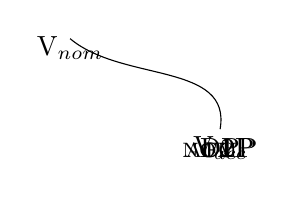
\begin{tikzpicture}[baseline,decoration={brace}]
\Tree [.\node(abovev){}; [.\node(V){V$_{nom}$}; ] 
[.\node(grow){}; ] ]
\begin{scope}[shift={(0.75in,-0.5in)}]
\Tree [.\node(bigtree){}; 
[.\node(Acc){\textsc{accP}};  [.\node(B){\textsc{f2}}; ]
[.\node(Nom){\textsc{nomP}};  [.\node(A){\textsc{f1}}; ]
[.\node(root){DP}; \edge[roof]; {} ] ] ] 
[ [.{...} ]
[.\node(V){V$_{acc}$}; ] ] ] ]
\end{scope}
\begin{scope}
\draw (grow.north) edge[out=320,in=80] (Nom.north);
\end{scope} 
\end{tikzpicture}

Next I discuss the situation in which the external case is more complex than the internal case, again accusative and nominative. A sentence from Old High German that illustrates this type of situation is given in \ref{ex:ohg-nom-acc-prev}, again repeated from earlier chapters.

\exg. Thíz ist then sie zéllent\\
\ac{dem}.\ac{sg}.\ac{n}.\ac{nom} be.\ac{pres}.3\ac{sg}\scsub{[nom]} \ac{rp}.\ac{sg}.\ac{m}.\ac{acc} 3\ac{pl}.\ac{m}.\ac{nom} tell.\ac{pres}.3\ac{pl}\scsub{[acc]}\\
`this is the one whom they talk about' \flushfill{Old High German, \ac{otfrid} III 16:50}\label{ex:ohg-nom-acc-prev}

The structure that corresponds to this sentence is given in \ref{ex:bergsma-nom-acc}. The relative clause on the right contains a predicate that takes nominative case, which appears on the left edge of the relative clause. The predicate in the main clause takes accusative case. The feature that makes the nominative an accusative is remerged with the nominative relative pronoun from the relative clause. The predicate from the main clause in turn is merged with the accusative node.

\ex.\label{ex:bergsma-nom-acc}
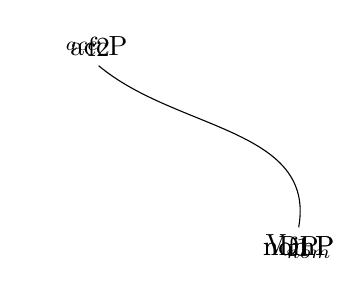
\begin{tikzpicture}[baseline,decoration={brace}]
\Tree [.\node(topnode){}; [.V$_{acc}$ ]
[.\node(Acc){\tsc{accP}}; [.\node(C){\tsc{f2}}; ] \edge[transparent];
[.\node(grow){}; ] ] ] ] ] ]
\begin{scope}[shift={(1.0in,-1.0in)}]
\Tree [.\node(free){\tsc{nomP}};
[.\node(Nom){\tsc{nomP}};  [.\node(A){\tsc{f1}}; ]
[.\node(root){DP}; \edge[roof]; {} ] ]
[ [.{...} ] 
[.\node(V){V$_{nom}$}; ] ] ]
\end{scope}
\draw (Acc.south) edge[out=320,in=80] (free.north);
\end{tikzpicture}

In sum, the account of \citet{bergsma2019} can be described in three derivational steps. 
In step 1, the relative clause predicate merges with the required case node. 
In step 2, the relative pronoun moves to the left edge of the clause. 
In step 3, the main clause predicate merges with the required case node. When the required case node is available, as in \ref{ex:bergsma-acc-nom}, this node is remerged with the main clause predicate. When the required case node is not available, as in \ref{ex:bergsma-nom-acc}, the highest case node is remerged with additional case features following the functional sequence until the required case node is merged, and then the main clause predicate is merged with the required case node. 

Variation between languages is formulated in terms of restrictions in step 3. A language without any restrictions is a language like Gothic: the relative pronoun always appears in the most complex case, no matter whether it is the internal or the external case. 

A language like Modern German has a restriction that is described as \textit{Keep spellout}: additional case features can only be merged to the relative pronoun if this does not change the spellout of the relative pronoun. As a result, when the internal case is more complex, a node within the relative pronoun can be remerged. However, when the internal case is less complex and additional case features need to be merged on top of the relative pronoun, this is prohibited. An exception is when it does not affect the spellout, which is how \citet{bergsma2019} accounts for syncretic forms being able to resolve a mismatch. 

A language like Polish has an additional restriction on top of the restriction that German has which is described as \textit{Only remerge highest node}: only the structurally highest node can be remerged with the main clause predicate. As a result, when the internal case is more complex, an embedded node cannot be remerged with the main clause predicate. Since Polish also has the restriction \textit{Keep spellout}, headless relatives with more complex external cases are also not grammatical, for the same reason as in Modern German.

\citet{bergsma2019} describes a fourth type of language, which is a language like Modern Greek, which is not described in this dissertation. This type of language only has the restriction \textit{Only remerge highest node} and not \textit{Keep spellout}. This means that headless relatives with a more complex internal case in Modern Greek are not grammatical, for the same reason as described for Polish above. When the external case is more complex, however, additional case features can be remerged with the relative pronoun. For Modern Greek this works in the same way as for languages like Gothic for the nominative/accusative cases. Exceptions are cases that involve a genitive. I give an example in \ref{ex:greek-nom-gen-prev}. We see the relative pronoun appearing in the case of the main clause (here nominative) and an additional resumptive pronoun in genitive appearing in the embedded clause, repeated from an earlier chapter. 

\exg. Me efχarístisan ópji tus íχa ðósi leftá.\\
 \ac{cl}.1\ac{sg}.\ac{acc} thank.\ac{pst}.3\ac{pl}\scsub{[nom]} \ac{rp}.\ac{pl}.\ac{m}.\ac{nom} \ac{cl}.3\ac{pl}.\ac{gen} have.\ac{pst}.1\ac{sg} give.\ac{ptcp}\scsub{[gen]} money\\
 `Whoever I had given money to, thanked me.'\flushfill{Modern Greek, adapted from \pgcitealt{daskalaki2011}{80}}\label{ex:greek-nom-gen-prev}

In a derivation similar to the ones discussed so far, this would mean that the relative pronoun first appears in the genitive case. Then when the main clause predicate requires a less complex case, part of the relative pronoun moves away to a place lower in the structure and spells out as a resumptive. This leaves a relative pronoun of which the highest node can be remerged. The movement of the resumptive pronoun is atypical, but the restrictions \textit{Keep spellout} and \textit{Only remerge highest node} fit the described pattern well.

This account and the one in this dissertation have in common how they model the case hierarchy: cases are represented by different nodes in the syntax and less complex cases are syntactically embedded in more complex cases. What differs is how the two accounts model the differences between languages. This starts with the assumptions about the underlying syntactic structure of the headless relative. The account in \citealt{bergsma2019} assumes that there is only a single element involved in case competition, which is the relative pronoun. Differences between languages follow from restrictions on whether the spellout of the relative pronoun can be changed and whether embedded features can be remerged. Unlike what is proposed in this dissertation, in which differences between languages follows from the internal structure of relative pronouns and light heads, these differences do not follow independently from properties of the language. There is no evidence from the morphology or from other constructions in a language that tells us whether the language has these restrictions, making them purely stipulative at this point. The account could be made stronger if there is evidence not from headless relatives that supports the need for the restrictions.


\section{Summary}

In this chapter I discussed three different proposals that account for different language types in headless relatives.
To account for the case facts, all of them refer in some way to a case hierarchy.
The accounts differ in how they model the variation between the languages. Of course there are differences in the mechanics of the proposals, but more importantly, there are differences in the empirical scope they have and the predictions they make.
What stands out is that all accounts except for the one in this dissertation include the Modern Greek pattern. Future research should point out how Modern Greek fits in the typology best and how the account set up in this dissertation can also account for this pattern.

\bookmarksetup{startatroot}
% !TEX root = thesis.tex

\chapter{Discussion}\label{ch:discussion}


\section{Diachronic part}

First, German only had the d-pronoun and attraction. The pattern of attraction that came with that pronoun is ext only.
At some point, German invented the wh-pronoun. Helmut showed how it emerged. With that came the other pattern: int only. Some people lost the attraction (but everybody kept the d-pronoun) and with that the pattern disappeared.
So the patterns in headless relatives follow from the relative pronouns in the language.

Why are all languages of the `matching' type dead languages?
Was it a common thing that wh-pronouns were not used as relative pronouns?

Wouldn't we now not expect that Modern German patterns with Old High German wrt attraction in headed constructions. Yes, we would. And yes, this is exactly what we see. Paper by Bader on case attraction.

First there was only the relative pronoun with a D. Then we did case competition with this one, in both directions. Later, we only did it with the wh, and we only had internal left. Because this competitor was introduced, the case competition with D disappeared.


\section{Towards deriving the always-external pattern}

grosu: morphological distinctions correlate with `freedom'

Why \tsc{fem} does not have \tsc{wh}-pronouns?


\section{More languages}

\tit{valita} `choose' takes a partitive object

\ex. Valitsen mista sina piddt.
choose-I.el what-el you like-you.part
'I choose what you like.'

\tit{pitää} `like' takes elative objects

\exg. *Pidan mista sind valitset.\\
like-I.part what-el you choose-you.el\\
`I like what you choose.'

\exg. *Pidan mita sind valitset.\\
like-I.part what-el you choose-you.el\\
`I like what you choose.'

\section{The missing dative/accusative}

The accusative/dative example is missing from Gothic, Old High German and Ancient Greek. What if I take that seriously?


%%%%
\backmatter

\clearpage
\chapter*{Primary texts}
\begingroup
  \setlength{\LTleft}{-\tabcolsep}
\printacronyms[include=texts, heading=none]
\endgroup
\addcontentsline{toc}{chapter}{Primary texts}

\newrefcontext[sorting=nyt]
\printbibliography
% \bibliography{references.bib} % for natbib

%%%%

\end{document}
